\chapter{Tool demonstration for lifetime-long depletion: Transatomic Power MSR}

This chapter presents a validation demonstration applying SaltProc v1.0 to 
the \gls{TAP} \gls{MSR}. The \gls{TAP} concept was selected because it is well 
analyzed in the literature \cite{betzler_two-dimensional_2017, 
betzler_assessment_2017-1} making code-to-code verification with 
ChemTriton/SCALE possible \cite{betzler_assessment_2017-1}. This chapter 
presents the \gls{TAP} \gls{MSR} core lifetime-long (25 years) depletion 
simulation with moderate time resolution (3-day depletion step) and a 
constant, 100\% power level. The results obtained with SaltProc v1.0 are 
compared with full-core \gls{TAP} depletion analysis by Betzler \emph{et al.} 
\cite{betzler_assessment_2017-1} with assumed ideal removal efficiency (100\% 
of the target isotope is removed). This validation effort showed that the 
SaltProc v1.0 solution matches the case with \emph{ideal extraction 
efficiency}. 

Finally, this chapter presents a lifetime-long fuel salt depletion simulation 
for the case with \emph{a realistic, physics-based} mathematical model for 
noble gas removal efficiency, which provides fuel isotopic composition 
evolution during 25 years of the \gls{TAP} \gls{MSR} operation. Additionally, 
this chapter presents safety and operational parameters evolution during 
operation. Detailed 
insights about fuel salt composition and neutron spectrum dynamics obtained 
herein will be used in the following chapters to investigate \gls{TAP} 
reactor poisoning during load-following.


\section{Transatomic Power MSR design description}\label{sec:tap_design_sum}

The \gls{TAP} concept is a 1250 MW$_{th}$ \gls{MSR} with a LiF-based uranium 
fuel salt \cite{transatomic_power_corporation_technical_2016}. This concept 
uses configurable zirconium hydride rods as the moderator, while most 
\gls{MSR} designs typically propose high-density reactor graphite. Zirconium 
hydride offers a much higher neutron moderating density than graphite, so, a 
much smaller volume of zirconium hydride is needed to achieve a thermal energy 
spectrum similar to one obtained with a graphite moderator. Moreover, 
zirconium hydride clad in a corrosion-resistant material has a much longer 
lifespan in extreme operational conditions (e.g., high temperature, large 
neutron flux, chemically aggressive salt) than reactor graphite 
\cite{transatomic_power_corporation_lost_2018}. Finally, zirconium hydride is 
a nonporous material and holds up fewer neutron poisons (e.g., xenon, krypton) 
than does high-density reactor graphite.

In this section, the design characteristics and reprocessing plant design are 
based on information presented in the TAP white papers  
\cite{transatomic_power_corporation_technical_2016,
transatomic_power_corporation_neutronics_2016} and \gls{ORNL} technical 
reports \cite{betzler_two-dimensional_2017, betzler_assessment_2017-1}.

\subsection{General design description}

Figure~\ref{fig:tap-rendering} renders of the primary and secondary loop of 
the \gls{TAP} \gls{MSR} seated inside a concrete nuclear island. 
Figure~\ref{fig:tap-primary-scheme} shows the schematic design of a 520 
MW$_{e}$, 2-loop nuclear reactor system with an intermediate salt loop.
\begin{figure}[h] % replace 't' with 'b' to 
	\centering
	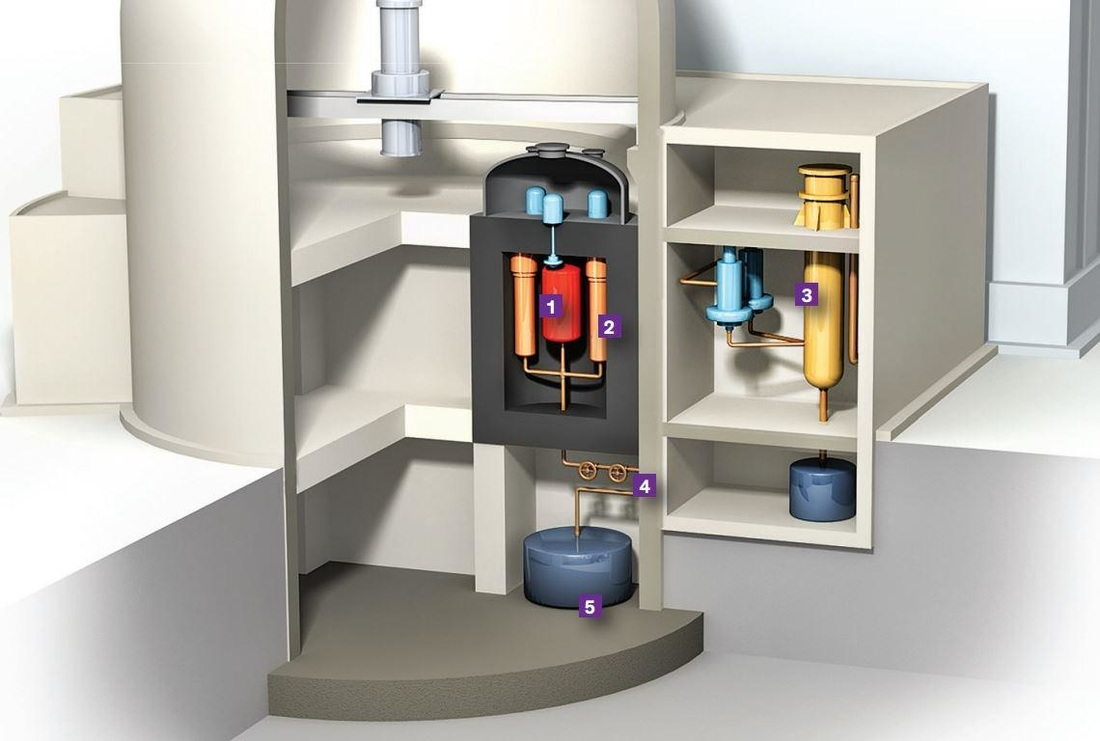
\includegraphics[width=\textwidth]{ch4/tap_render.jpg}
	\caption{Rendering of the \gls{TAP} \gls{MSR}. The fission happens in the 
		fuel salt inside the reactor vessel (1). The heat generated by a
		self-sustaining nuclear fission reaction would be transferred to the 
		secondary salt by heat exchangers (2), which would boil water in the 
		steam generator (3). Valves made of salt with a higher melting point 
		(4) would melt in case of emergency, allowing the salt to drain into a 
		drain tank (5), which can passively dissipate decay heat	
		(reproduced from 
		\cite{strickland_transatomic_2014}, illustration by Emily Cooper).}
	\label{fig:tap-rendering}
\end{figure}
\begin{figure}[h] % replace 't' with 'b' to 
	\centering
	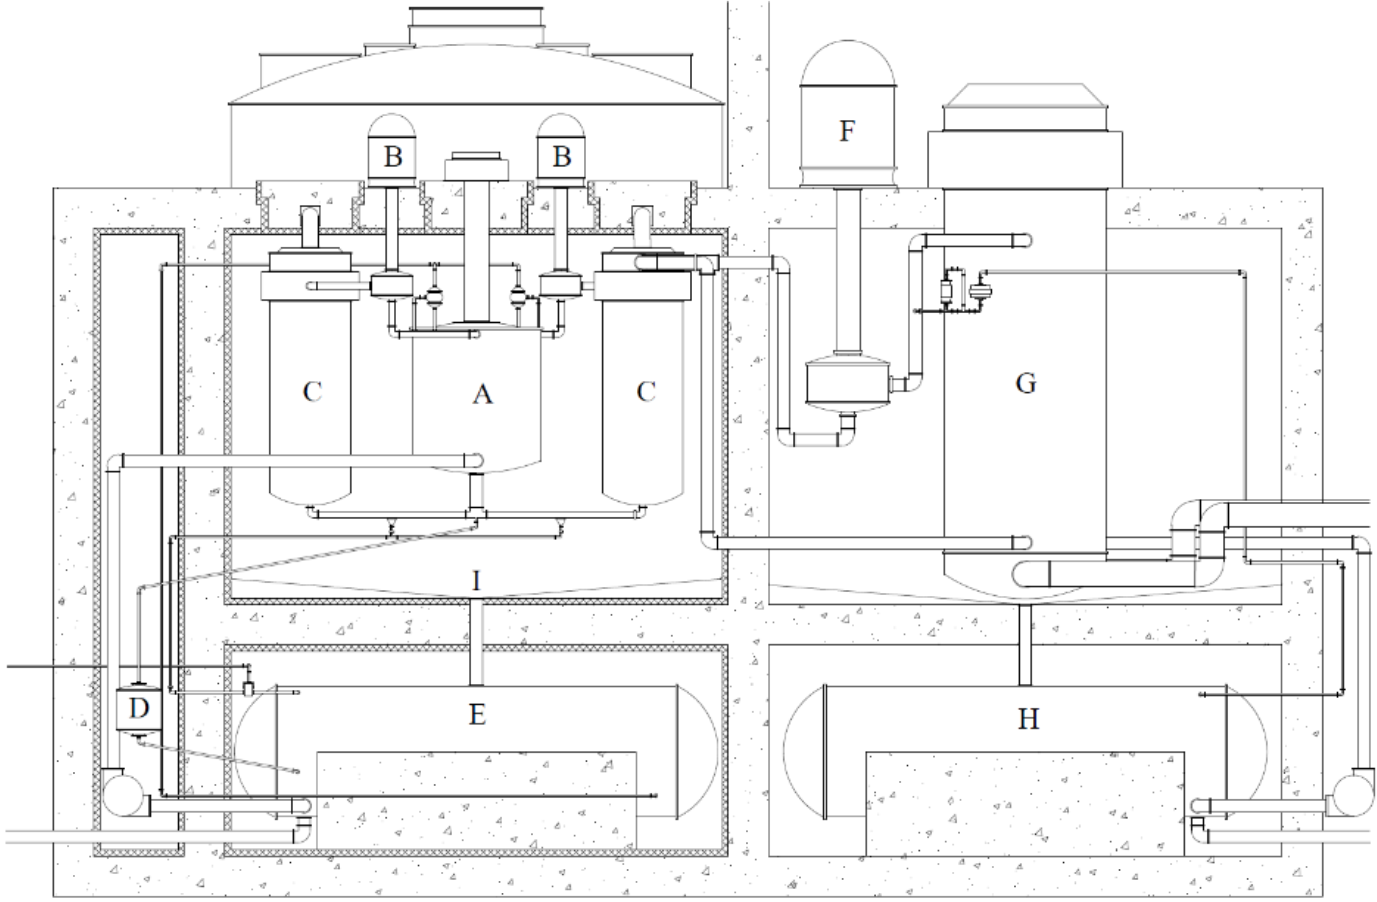
\includegraphics[width=\textwidth]{ch4/tap_simplified_scheme.png}
	\caption{Simplified schematic of the \gls{TAP} \gls{MSR} primary and  
		secondary loops (reproduced from the Transatomic Power Technical White 
		Paper \cite{transatomic_power_corporation_technical_2016}). Figure 
		legend: 
		A) reactor vessel, B) fuel salt pumps, C) primary heat exchangers, D) 
		freeze plug, E) primary loop drain tank, F) secondary loop salt pump, 
		G) 
		steam generator, H) secondary loop drain tank, I) fuel catch basin.}
	\label{fig:tap-primary-scheme}
\end{figure}

The \gls{TAP} core design (Figure~\ref{fig:tap-side-view}) is very similar to 
the
original \gls{MSRE} design developed by \gls{ORNL} 
\cite{haubenreich_experience_1970} but has two significant innovations: 
the fuel salt composition and the moderator. The \gls{MSRE}'s 
LiF-BeF$_2$-ZrF$_4$-UF$_4$ salt has been substituted with LiF-UF$_4$ salt, 
which allows for an increase in the uranium concentration within the fuel salt 
from 0.9 to 27.5\% while maintaining a relatively low melting point 
(490$^{\circ}$C compared with 434$^{\circ}$C for the original \gls{MSRE}'s 
salt) \cite{betzler_two-dimensional_2017}. The graphite has an extensive 
thermal scattering cross section which makes it a perfect moderator but has 
a few major drawbacks: 
\begin{enumerate}[label=(\alph*), noitemsep, topsep=0pt]
	\item low lethargy gain per collision requires a large volume of a
	moderator to be present to reach criticality, which leads to a larger core 
	and obstructs the core power density;
	\item even special reactor-grade graphite has relatively high porosity; 
	thus, it holds gaseous \glspl{FP} (e.g., tritium, xenon) in pores;
	\item reactor graphite lifespan in a commercial reactor is 
	approximately ten years \cite{robertson_conceptual_1971}.
\end{enumerate}
As previously mentioned, to resolve these issues, the \gls{TAP} concept uses 
zirconium hydride instead of graphite, allowing for a more compact core and a 
significant increase in power density. These two innovative design choices, 
together with a configurable moderator (the moderator-to-fuel ratio can be 
changed during operation), facilitate use of commercially available 5\% 
enriched \gls{LEU} fuel cycle. 
\begin{figure}[h] % replace 't' with 'b' to 
	\hspace{+2.2in}
	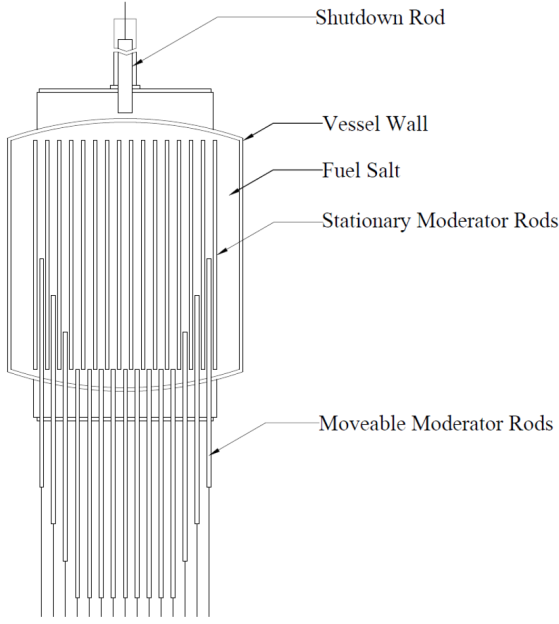
\includegraphics[width=0.65\textwidth]{ch4/tap_front_view.png}
	\caption{The \gls{TAP} \gls{MSR} schematic view showing moveable moderator 
		rod bundles and shutdown rod (reproduced from Transatomic Power 
		White Paper \cite{transatomic_power_corporation_technical_2016}).}
	\label{fig:tap-side-view}
\end{figure}

The \gls{TAP} \gls{MSR} primary loop contains the reactor core volume  
(including the zirconium hydride moderator rods with silicon carbide  
cladding), pumps, pipes, and primary heat exchangers. Pumps circulate the  
LiF-(Act)F$_4$ fuel salt through the primary loop. The pumps, vessels, tanks, 
and piping are made of a nickel-based alloy (similar to Hastelloy-N\footnote{ 
Hastelloy-N is very common in \gls{MSR} designs now, but was developed at 
\gls{ORNL} in the \gls{MSRE} program that started in the 1950s.}), which 
is highly resistant to corrosion in various molten salt environments. Inside 
the reactor vessel, near the zirconium hydride moderator rods, the fuel salt 
is in a critical configuration and generates heat. Table~\ref{tab:tap_tab} 
contains details of the \gls{TAP} system design, which are taken from a
technical white paper \cite{transatomic_power_corporation_technical_2016} and 
a neutronics overview \cite{transatomic_power_corporation_neutronics_2016} as 
well as an \gls{ORNL} analysis of the \gls{TAP} design 
\cite{betzler_two-dimensional_2017, betzler_assessment_2017-1}. 
%%%%%%%%%%%%%%%%%%%%%%%%%%%%%%%%%%%%%%%%
\begin{table}[h!]
	\caption{Summary of principal data for the \gls{TAP} \gls{MSR} 
		(reproduced from \cite{betzler_assessment_2017-1, 
		transatomic_power_corporation_technical_2016}). }
		\centering
	\begin{tabularx}{0.8\textwidth}{L R}
		\hline
		Thermal power   		& 1250 MW$_{th}  $       		\\ 
		Electric power		    & 520 MW$_e  $ 			 		\\ 
		Gross thermal efficiency& 44\%     				 		\\  
		Outlet temperature      & 620$^{\circ}$C         		\\ 
		Fuel salt components    & LiF-UF$_4$				    \\  
		Fuel salt composition   & 72.5-27.5 mole\%				\\  
		Uranium enrichment      & 5\% $^{235}$U          	    \\
		Moderator               & Zirconium hydride (ZrH$_{1.66}$) rods \\
								& (with silicon carbide cladding)       \\
		Neutron spectrum 		& epithermal \\
		\hline
	\end{tabularx}
	\label{tab:tap_tab}
\end{table}
%%%%%%%%%%%%%%%%%%%%%%%%%%%%%%%%%%%%%%%%%%%%%%%%%%%%%%%%%%%%%%%%%%%%%%%%%%%%%%%

\subsection{Reactor core design}
In the \gls{TAP} core (Figure~\ref{fig:tap-core-ben}), fuel salt flows around 
moderator assemblies consisting of lattices of zirconium hydride rods clad in 
a corrosion-resistant silicone carbide. The \gls{TAP} reactor pressure vessel 
is a cylinder made of a nickel-based alloy with an inner radius of 150 cm, a 
height of 350 cm, and a wall thickness of 5 cm. 
\begin{figure}[t] % replace 't' with 'b' to 
	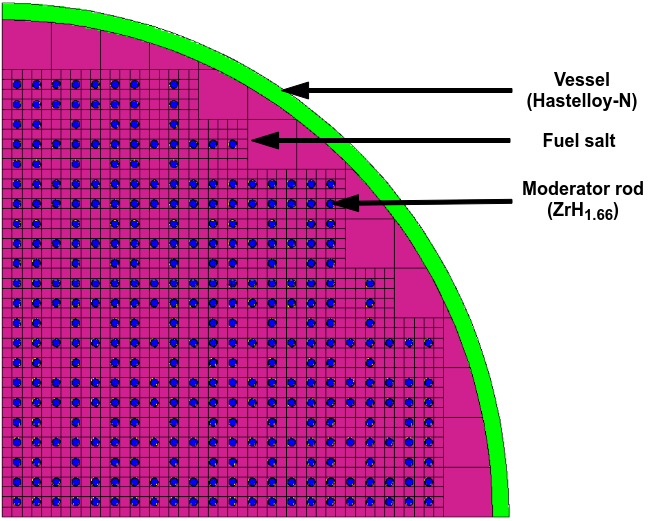
\includegraphics[width=\textwidth]{ch4/tap_core_ornl.png}
	\vspace{-0.1in}
	\caption{The \gls{TAP} \gls{MSR} schematic core view showing moderator 
		rods (reproduced from ORNL/TM-2017/475  
		\cite{betzler_assessment_2017-1}).}
	\label{fig:tap-core-ben}
\end{figure}

The \gls{SVF} in the core is a parameter similar to the widely-used 
moderator-to-fuel ratio and can be defined as:
\begin{align}
SVF &= \frac{V_F}{V_F+V_M} = \frac{1}{1+V_M/V_F}
\intertext{where}
V_F &= \mbox{fuel volume $[m^3]$} \nonumber \\
V_M &= \mbox{moderator volume $[m^3]$} \nonumber \\
V_M/V_F &= \mbox{moderator-to-fuel salt ratio $[-]$.} \nonumber
\end{align}

Figure~\ref{fig:svf-predetermined} shows the \gls{SVF} variation during  
operation that shifts the reactor neutron energy spectrum from intermediate to 
thermal to maximize fuel burnup. At the \gls{BOL}, a high \gls{SVF} results in 
a relatively hard spectrum and enhances fertile material ($^{238}$U) 
conversion into the fissile material ($^{239}$Pu) when the startup fissile 
material ($^{235}$U) inventory is still large. As fissile concentration in the 
fuel salt declines, additional moderator rods are introduced to maintain 
criticality, leading to salt volume fraction decrease (see 
Figure~\ref{fig:svf-predetermined}).

The initial \gls{TAP} concept suggested varying the \gls{SVF} by inserting 
fixed-sized moderator rods via the bottom of the reactor vessel (for safety 
considerations), similar to moving the control rods in a \gls{BWR}, as shown 
in Figure~\ref{fig:tap-side-view} 
\cite{transatomic_power_corporation_neutronics_2016}. The later \gls{TAP} 
concept proposes reducing the \gls{SVF} by reconfiguring the moderator rods 
during the regular shutdown for reactor maintenance 
\cite{betzler_assessment_2017-1}. For the \gls{TAP} reactor, \gls{EOL} occurs 
when the maximum number of moderator rods is inserted into the core and a 
further injection of fresh fuel salt does not alter criticality. Unmoderated 
salt flows in the annulus between the core and the vessel wall to reduce fast 
neutron fluence at the vessel structural material.
\begin{figure}[t] % replace 't' with 'b' to 
	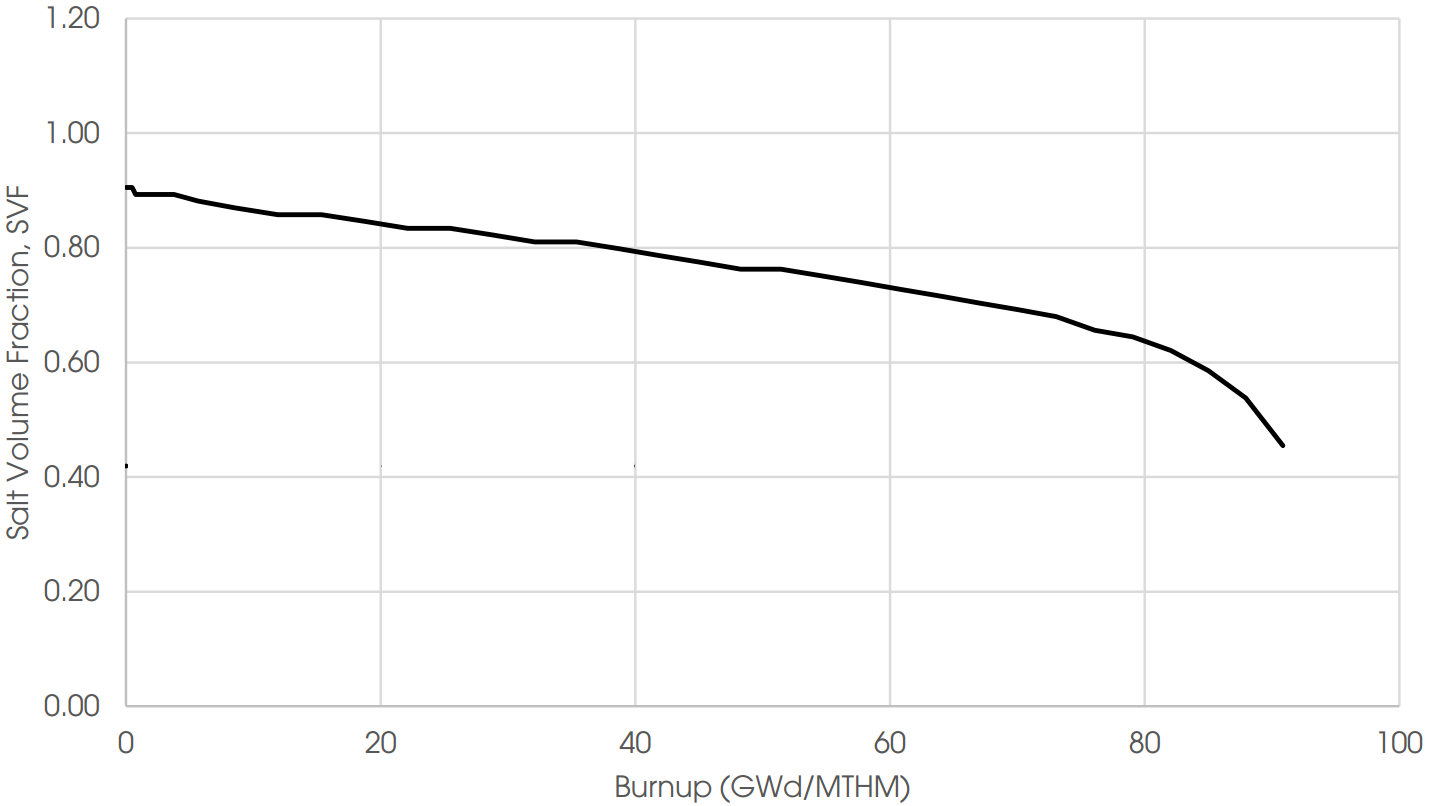
\includegraphics[width=\textwidth]{ch4/svf_predetermined.png}
	\caption{The change in SVF as a function of burnup in the \gls{TAP} 
	reactor (reproduced from Transatomic Power Neutronics Overview  
	\cite{transatomic_power_corporation_neutronics_2016}).}
	\label{fig:svf-predetermined}
\end{figure}


\subsection{Fuel salt reprocessing system}
The \gls{TAP} nuclear system contains a fission product removal system. 
Gaseous \glspl{FP} are continuously removed using an off-gas system, while 
liquid and solid \glspl{FP} are extracted via a chemical processing system. As 
these byproducts are gradually removed, a small quantity of fresh fuel salt is 
regularly added to the primary loop. This process conserves a constant fuel 
salt mass and keeps the reactor critical. In contrast with the \gls{MSBR} 
reprocessing system, the \gls{TAP} design does not need a protactinium 
separation and isolation system because it operates in a uranium-based 
single-stage fuel cycle. The authors of the \gls{TAP} concept suggested three 
distinct fission product removal methods 
\cite{transatomic_power_corporation_neutronics_2016}:
\paragraph*{Off-Gas System:} The off-gas system removes gaseous fission 
products such as krypton and xenon, which are then compressed and temporarily 
stored until they have decayed to the background radiation level. Trace 
amounts of tritium are also removed and bottled in a liquid form via the same 
process. Also, the off-gas system directly removes a small fraction of the 
noble metals.
\paragraph*{Metal Plate-Out/Filtration:} A nickel mesh filter removes noble 
and semi-noble metal solid fission products as they plate out onto the 
internal surface of the filter.
\paragraph*{Liquid Metal Extraction:} Lanthanides and other non-noble metals 
stay dissolved in the fuel salt. They generally have a lower capture cross 
section and thus absorb fewer neutrons than $^{135}$Xe, but their extraction 
is essential to ensure normal operation. In the \gls{TAP} reactor, lanthanide 
removal is accomplished via a liquid-metal/molten salt extraction process 
similar to that developed for the \gls{MSBR} by \gls{ORNL}  
\cite{robertson_conceptual_1971}. This process converts the dissolved 
lanthanides into a well-understood oxide waste form, similar to that of 
\gls{LWR} \gls{SNF}. This oxide waste exits the \gls{TAP} reprocessing 
plant in ceramic granules which can be sintered into another convenient form 
for storage \cite{transatomic_power_corporation_technical_2016}.\\

Figure~\ref{fig:tap-reproc} shows the principal design of the \gls{TAP} 
primary loop, including an off-gas system, nickel mesh filter, and lanthanide 
chemical extraction facility. As in the \gls{MSBR}, the \gls{TAP} off-gas 
system is based on helium sparging through the fuel salt with consequent gas 
bubbles removed before returning the fuel salt to the core (see 
Section~\ref{sec:gas-separ}). 
Nevertheless, one crucial difference must be noted: the \gls{MSBR} gas 
separation system suggested helium injection and subsequent transport of the 
voids throughout the primary loop, including the core for at least ten full 
loops \cite{robertson_conceptual_1971}. 
\begin{figure}[htp!] % replace 't' with 'b' to 
	\centering
	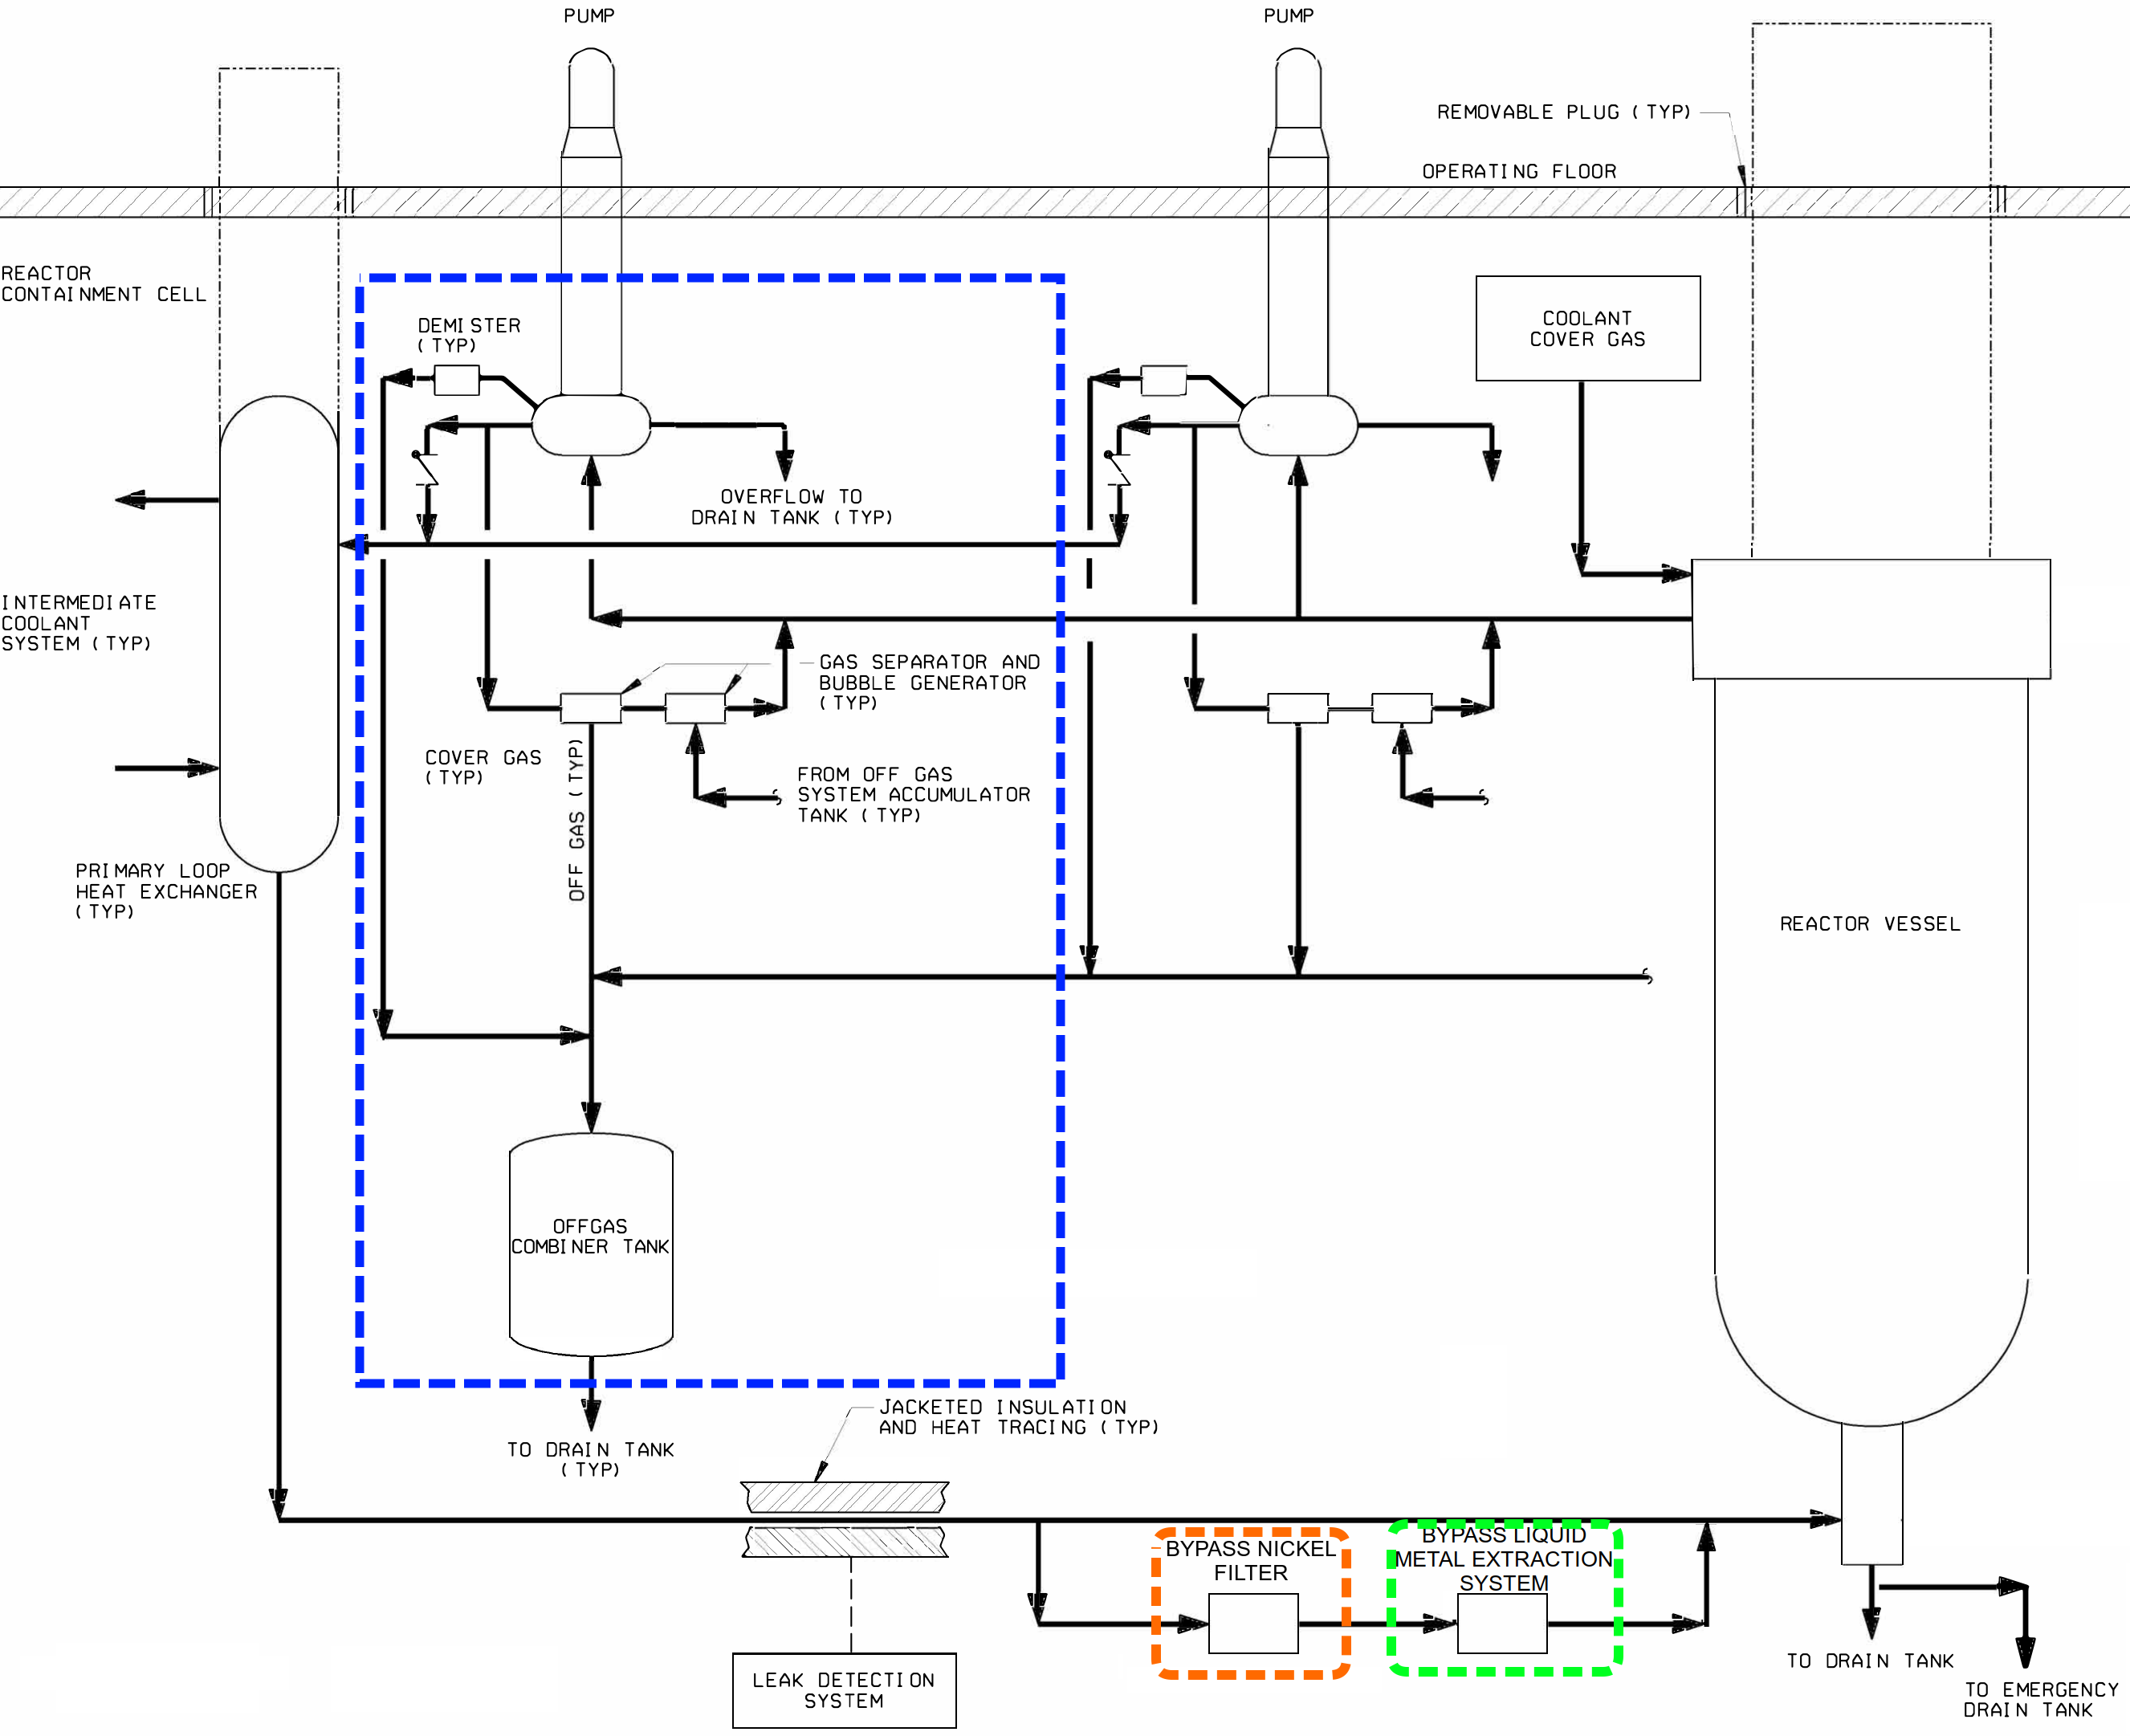
\includegraphics[width=\textwidth]{ch4/tap_primary_loop.png}
	\caption{Simplified \gls{TAP} primary loop design including off-gas system 
		(blue), nickel filter (orange), and liquid metal extraction system 
		(green) (reproduced from \cite{transatomic_power_transatomic_2019}).}
	\label{fig:tap-reproc}
\end{figure}

In the \gls{TAP} design the introduction of the void (helium bubbles) during 
operation is a significant concern for safe, stable operation because the 
increase of void fraction in the fuel salt when it enters back to the core 
could cause unpredictable reactivity change. Kedl stated without explanation, 
``Average loop void fractions as high as 1\% are undesirable... it is 
desirable to keep the average loop void fraction well below 
1\%.''\cite{robertson_conceptual_1971} The \gls{MSBR} design targeted a 0.2\% 
average void in the fuel salt \cite{robertson_conceptual_1971} and the 
\gls{MSRE} successfully operated with an average void fraction of about 0.7\% 
\cite{compere_fission_1975}. The \gls{TAP} design reduces void fraction in the 
fuel salt to negligible levels by using an effective gas separator for 
stripping helium/xenon bubbles before returning the salt to a primary loop 
(Figure~\ref{fig:tap-reproc}, blue block). 

Noble and semi-noble metal solid fission products tend to plate out onto metal 
surfaces, including piping, heat exchanger tubes, reactor vessel inner 
surface, etc. Previous research by \gls{ORNL} \cite{robertson_conceptual_1971} 
reported that about 50\% of noble and semi-noble metals would plate out inside 
\gls{MSBR} systems (including the off-gas system) without any special 
treatment. To improve the extraction efficiency of these fission products, the 
\gls{TAP} concept suggested employing a nickel mesh filter located in a bypass 
stream in the primary loop (Figure~\ref{fig:tap-reproc}, orange block). The 
main idea of this filter is to create a large nickel surface area using porous 
metal (e.g., Inconel fibers). The fuel salt flows throughout the filter 
and noble metals plate out on the filtering material. 

This Liquid Metal Extraction process for the \gls{TAP} concept has been 
adopted from the \gls{MSRE}. The \gls{MSRE} demonstrated a liquid-liquid 
extraction process for removing rare earths and lanthanides from fuel salt and 
estimated efficiency of this process. In fact, due to similarities in 
reprocessing schemes, the \gls{TAP} project reported almost the same set of 
elements for removal and similar effective cycle times\footnote{The \gls{MSBR} 
program defined ``cycle time" as the time required to remove 100\% of atoms of 
a target nuclide from a
fuel salt \cite{robertson_conceptual_1971}.
} as 
suggested for the \gls{MSBR} (Table~\ref{tab:reprocessing_list}). The 
\gls{TAP} neutronics white paper specifies additional low-probability fission 
products and gases that should be removed during operation  
\cite{transatomic_power_corporation_neutronics_2016}. These elements are 
categorized into the previously defined processing groups, but the removal 
rates of most of these elements (except hydrogen) are meager.

Details of gas removal and fuel reprocessing systems have historically 
been conceptual. Accordingly, liquid-fueled system design, including the 
\gls{TAP} concept, usually assumes ideal (rather than realistically 
constrained) removal efficiencies for reactor performance simulations. In this 
thesis, I developed a realistic online reprocessing system and reactor model 
to capture the dynamics of fuel composition evolution during reactor 
operation. Gas removal efficiency is variable in that model, described using 
mathematical correlations from Chapter 2 (see Equation~\ref{eq:gas_eff}). For 
the other \glspl{FP}, a fixed\footnote{Published information about dynamics of 
extraction efficiency during reactor operation for noble-, semi-noble metals, 
and rare earths is insufficient to inform a variable removal efficiency.}, 
non-ideal extraction efficiency based on cycle time from  
Table~\ref{tab:reprocessing_list} was used to inform the fuel reprocessing 
model.

%%%%%%%%%%%%%%%%%%%%%%%%%%%%%%%%%%%%%%%%
\begin{table}[htp!]
	\centering
	\caption{The effective cycle times for fission product removal  from the 
		\gls{TAP} reactor (reproduced from \cite{betzler_implementation_2017} 
		and 
		\cite{transatomic_power_corporation_neutronics_2016}).}
	\begin{tabular}{p{0.2\textwidth} p{0.42\textwidth} p{0.12\textwidth} 
			p{0.14\textwidth}}
		\hline 
		%\begin{tabularx}{\linewidth}{l X} \toprule 
		\textbf{Processing group} & \qquad\qquad\qquad \textbf{Nuclides} & 
		\textbf{Removal rate (s$^{-1}$)} & \textbf{Cycle time (at full power)} 
		\\ [5pt] \hline 
		\multicolumn{3}{c}{\textit{Elements removed in the \gls{MSBR} concept 
		and adopted for the \gls{TAP}} \cite{robertson_conceptual_1971}} \\
		Volatile gases & Xe, Kr								  & 5.00E-2 & 20 
		sec \\ [5pt]
		Noble metals & Se, Nb, Mo, Tc, Ru, Rh, Pd, Ag, Sb, Te & 5.00E-2 & 20 
		sec \\ [5pt]
		Semi-noble metals & Zr, Cd, In, Sn	  				  & 5.79E-8 & 200 
		days \\ [5pt]
		Volatile fluorides & Br, I 							  & 1.93E-7 & 60 
		days \\ [5pt]
		Rare earths & Y, La, Ce, Pr, Nd, Pm, Sm, Gd           & 2.31E-7 & 50 
		days \\ [5pt]
		\qquad & Eu & 2.32E-8 & 500 days \\ [5pt]
		Discard & Rb, Sr, Cs, Ba & 3.37E-9 & 3435 days \\ [5pt] 
		\hline
		
		\multicolumn{3}{c}{\textit{Additional elements removed} 
			\cite{transatomic_power_corporation_neutronics_2016, 
				betzler_implementation_2017}  } \\
		Volatile gases & H								  	& 5.00E-2 & 20 
		sec    \\ [5pt]
		Noble metals & Ti, V, Cr, Cu						& 3.37E-9 & 3435 
		days \\ [5pt]
		Semi-noble metals & Mn, Fe, Co, Ni, Zn, Ga, Ge, As   & 3.37E-9 & 3435 
		days \\ [5pt]
		Rare earths & Sc									& 3.37E-9 & 3435 
		days \\ [5pt]
		Discard & Ca										& 3.37E-9 & 3435 
		days \\ [5pt] 
		\hline
	\end{tabular}
	\label{tab:reprocessing_list}
	\vspace{-0.9em}
\end{table}
%%%%%%%%%%%%%%%%%%%%%%%%%%%%%%%%%%%%%%%%%%%%%%%%%%%%%%%%%%%%%%%%%%%%%%%%%%%%%%%


\section{TAP system model} \label{sec:tap_model}
In this section, the \gls{TAP} core and fuel salt reprocessing system models  
for demonstrating SaltProc v1.0 are described in detail. I used these models 
for SaltProc demonstration and validation in the current and following 
chapters.

\subsection{Serpent 2 full-core model} 
Nested and lattice geometry types, as well as transformation capabilities of 
Serpent \cite{leppanen_serpent_2014}, are employed to represent the \gls{TAP} 
core. Figure~\ref{fig:tap-serpent-plan} shows the $XY$ section of the 
whole-core model at the expected reactor operational level when all control 
rods are fully withdrawn. Figures~\ref{fig:tap-serpent-elev} and 
\ref{fig:tap-serpent-elev-zoom} show a longitudinal section of the 
reactor. This model contains the moderator rods with their silicon carbide 
cladding, the pressure vessel, and the inlet and outlet plena 
(Table~\ref{tab:tap_model_param}). 
Fuel salt flows around square moderator assemblies consisting of lattices 
of small-diameter zirconium hydride rods in a corrosion-resistant material. 
The salt volume fraction for Figure~\ref{fig:tap-serpent-plan} is 0.917204, 
which means the modeled core is under-moderated and has an intermediate 
neutron spectrum. Quarter-core configurations of the \gls{TAP} core with 
various salt volume fractions, used in the current work to maintain 
criticality for a reasonable operational period ($>20$ years), are listed in 
Table~\ref{tab:tap_adjustable_core}, Figures~\ref{fig:tap-406-681}, and 
\ref{fig:tap-840-1668} in Appendix~A.
\begin{figure}[htp!] % replace 't' with 'b' to 
	\centering
	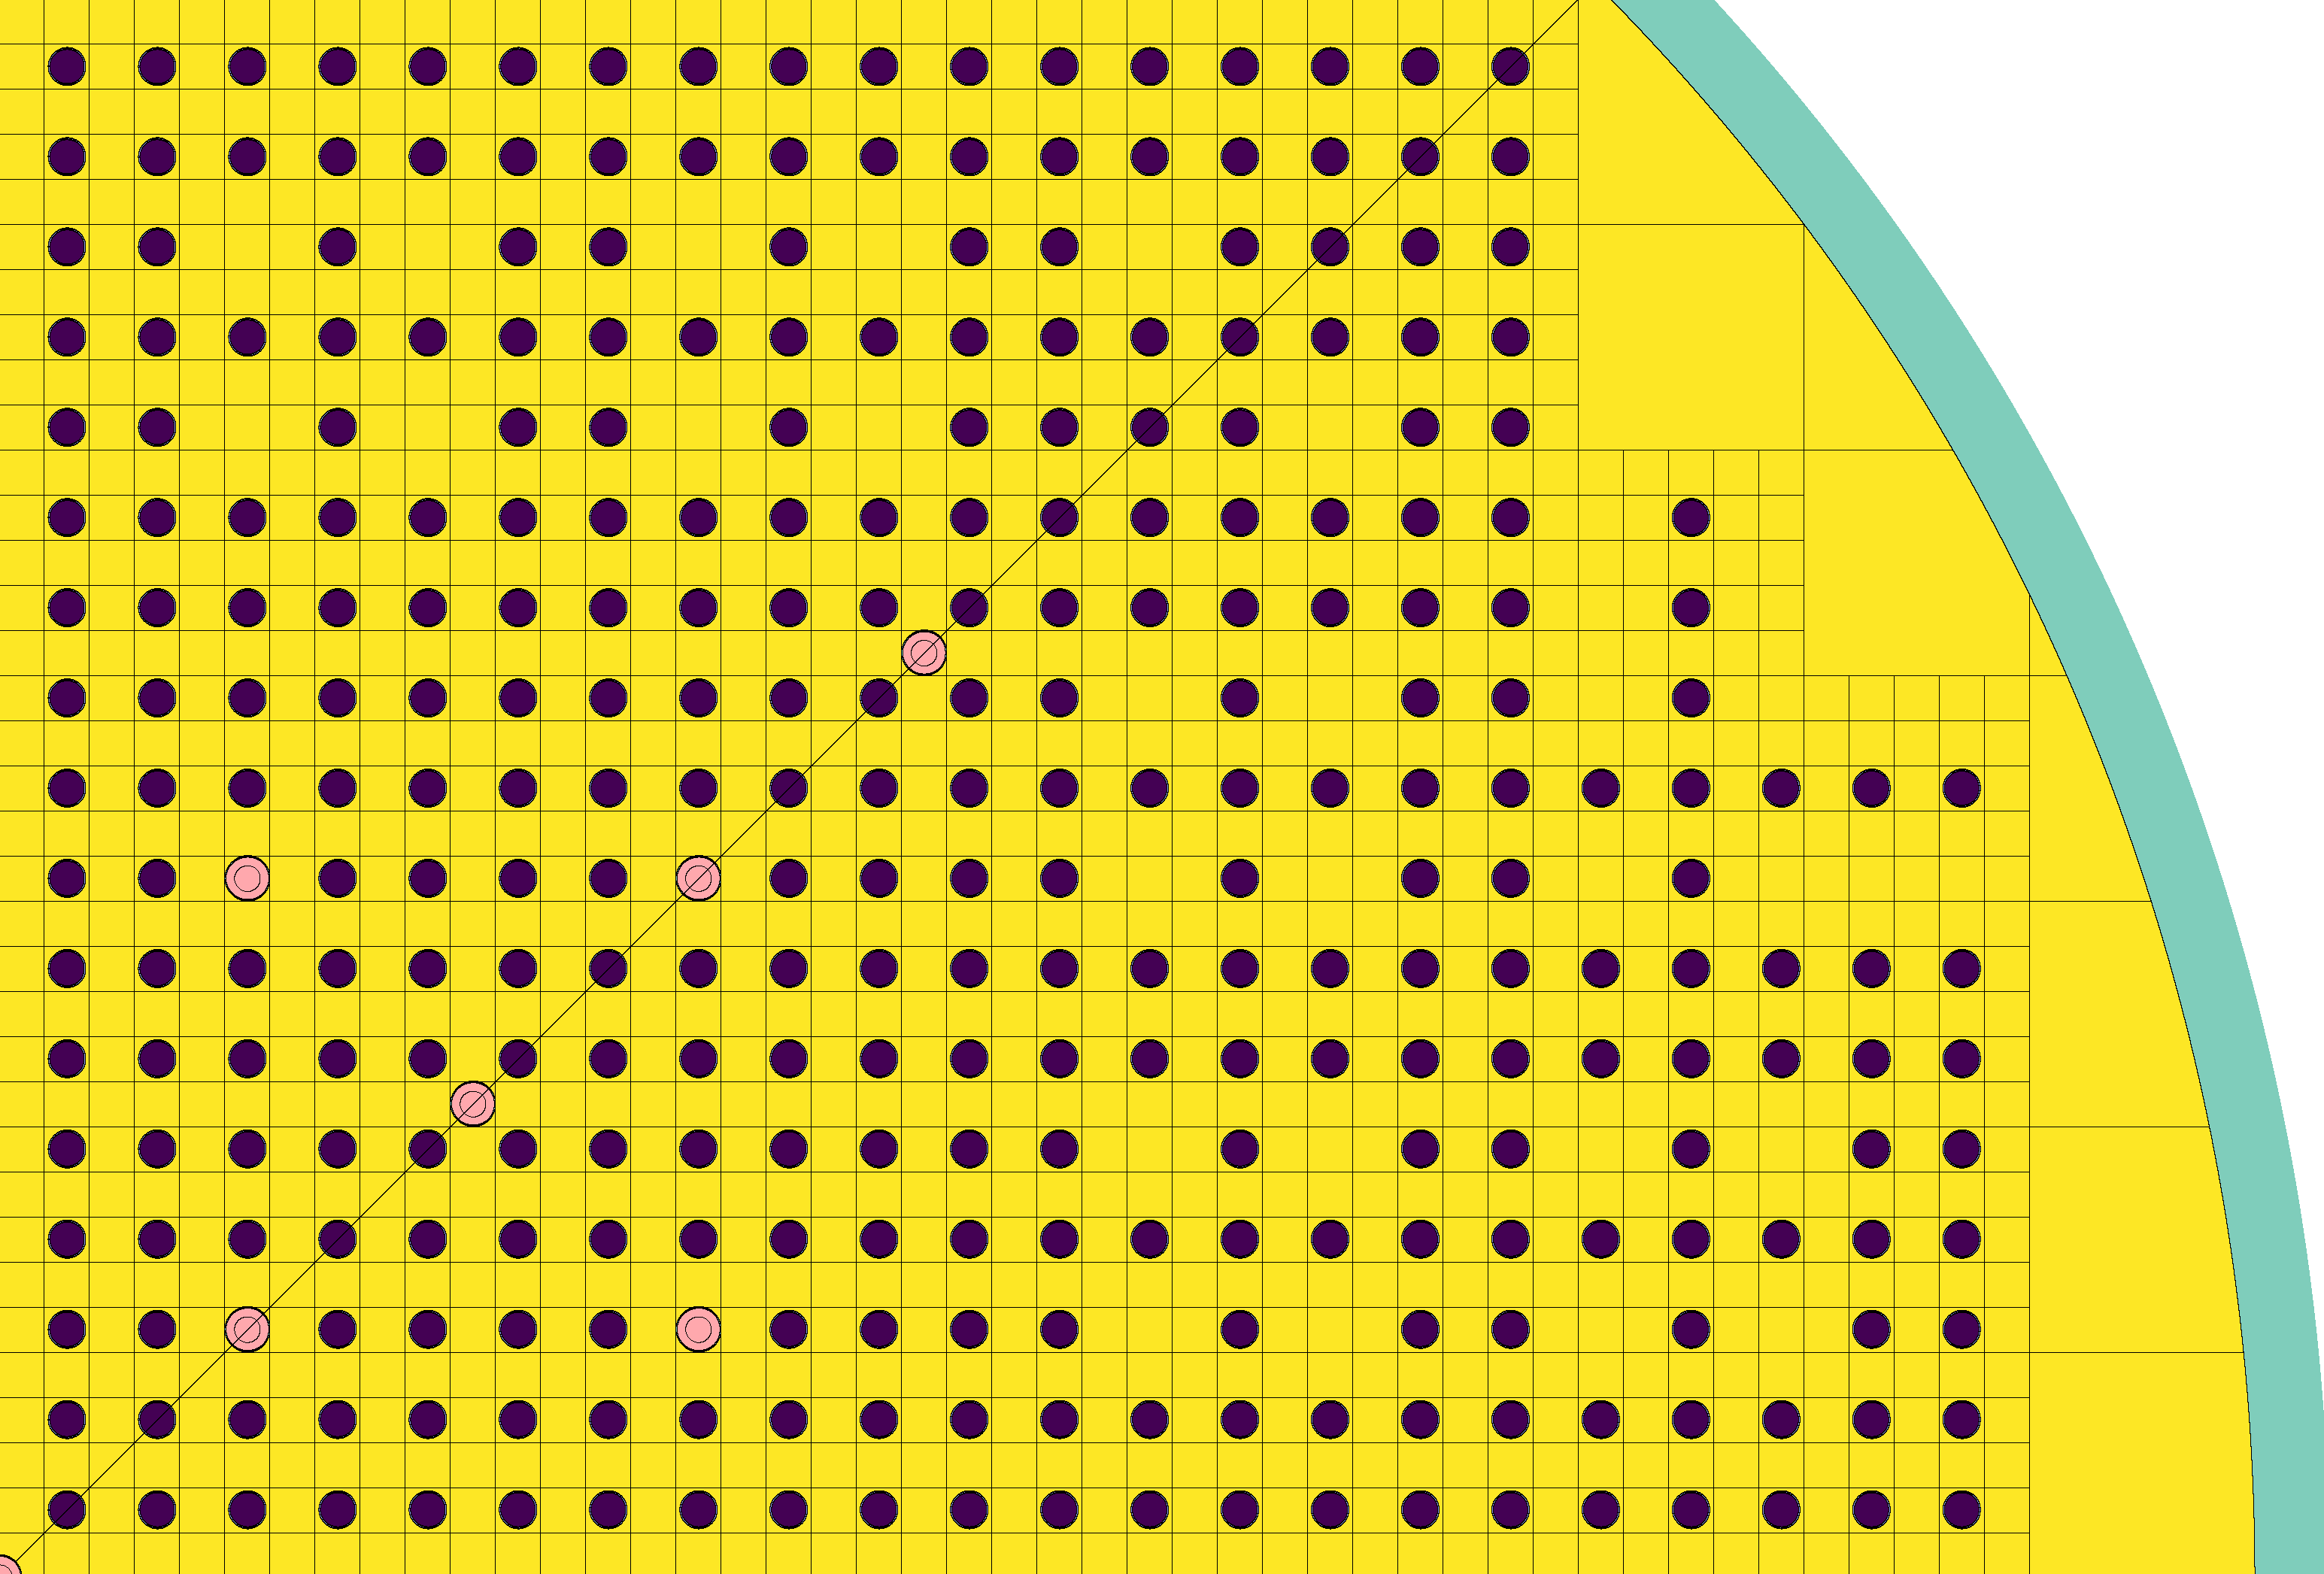
\includegraphics[width=0.75\textwidth]{ch4/tap_plan_view_serpent_347.png}
	\caption{An $XY$ section of the \gls{TAP} model at horizontal midplane 
		with fully withdrawn control rods at \gls{BOL} (347 moderator rods, 
		salt volume fraction 0.917204).}
	\label{fig:tap-serpent-plan}
\end{figure}

\begin{figure}[htp!] % replace 't' with 'b' to 
	\centering
	
\includegraphics[width=0.6\textwidth]{ch4/tap_elev_view_serpent_347.png}
	\caption{45$^{\circ}$ $XZ$ section of the \gls{TAP} core model.}
	\label{fig:tap-serpent-elev}
\end{figure}

To represent the reactivity control system, the model has: 
\begin{enumerate}[label=(\alph*), noitemsep, topsep=0pt]
	\item control rod guide tubes made of nickel-based alloy;
	\item control rods represented as boron carbide (B$_4$C) cylinders 
	with a thin Hastelloy-N coating;
	\item air inside guide tubes and control rods.
\end{enumerate}
The control rods must be able to suppress excess reactivity at the \gls{BOL} 
when the core configuration is the most reactive, and the neutron spectrum is 
the hardest. The control rod design shown on 
Figures~\ref{fig:tap-serpent-plan}, \ref{fig:tap-serpent-elev}, and 
\ref{fig:tap-serpent-elev-zoom} is comprised of a cluster of 25 rods that 
provide a total reactivity worth of $3922\pm10pcm$ at the \gls{BOL}.

\begin{figure}[htp!] % replace 't' with 'b' to 
	\centering
	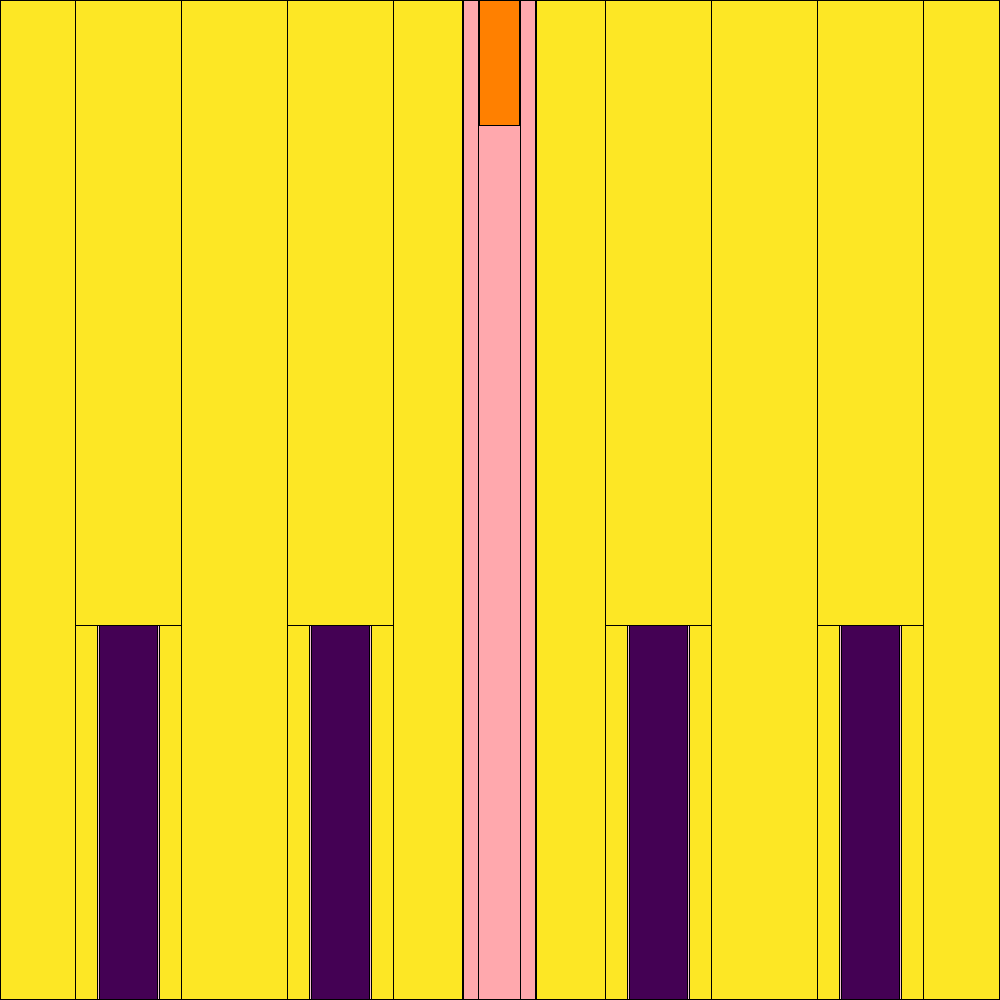
\includegraphics[width=0.55\textwidth]{ch4/tap_elev_view_zoomed_serpent.png}
	\caption{Zoomed $XZ$ section of the top of the moderator and control rods  
		in the \gls{TAP} model.}
	\label{fig:tap-serpent-elev-zoom}
\end{figure}
%%%%%%%%%%%%%%%%%%%%%%%%%%%%%%%%%%%%%%%%%%%%%%%%%%
\begin{table}[ht!]
	\caption{Geometric parameters for the full-core 3D model of the 
		\gls{TAP} (reproduced from Betzler \emph{et al.} 
		\cite{betzler_assessment_2017-1}). }
	\centering
	\begin{tabularx}{0.9\textwidth}{s s x p{0.14\textwidth}}
		\hline
		\textbf{Component}&\textbf{Parameter}&\textbf{Value}& \textbf{Unit}   
		\\ \hline
		\multirow{4}{*}{\begin{tabular}[c]{@{}l@{}}Moderator\\ 
				rod\end{tabular}} 
		& Cladding thickness      	  			    & 0.10 & cm				 
		\\  
		& Radius 				      	  			& 1.15 & cm				 
		\\  
		& Length				      	  			& 3.0  & m				 
		\\  
		& Pitch				      	  			& 3.0  & cm  			 \\ 
		\hline 
		
		\multirow{2}{*}{\begin{tabular}[c]{@{}l@{}}Moderator\\ 
				assembly\end{tabular}} 
		& Array				      	  			& 5 $\times$ 5 & 
		rods$\times$rods \\  
		& Pitch				      	  			& 15.0 & cm    				 
		\\  \hline
		
		\multirow{4}{*}{\begin{tabular}[c]{@{}l@{}}Core\end{tabular}}          
		& Assemblies  				   	  			& 268  & assemblies/core 
		\\  
		& Inner radius			      	  			& 1.5  & 
		m    				 \\  
		& Plenum height			   	  			& 25.0 & cm    				 
		\\  
		& Vessel wall thickness     	  			& 5.0 & 
		cm    				 \\ \hline            
	\end{tabularx}
	\label{tab:tap_model_param}
\end{table}
%%%%%%%%%%%%%%%%%%%%%%%%%%%%%%%%%%%%%%%%%%%%%%%%

The control rod cluster is modeled using the \textbf{TRANS} Serpent 2 feature, 
which allows the user to change the control rod position during the 
simulation easily. The current work assumed that all control rods are fully 
withdrawn from the core (Figure~\ref{fig:tap-serpent-elev-zoom}), but the user 
can use reactivity control capabilities in SaltProc v1.0 to change control 
rod position during operation. In this dissertation, all figures of the core 
were generated using the built-in Serpent plotter.

The neutron population per cycle and the number of active/inactive cycles were 
chosen to obtain a balance between minimizing uncertainty for a transport 
problem (28 pcm for $k_{eff}$) and simultaneously minimizing computational 
time.


\subsection{Model of the fuel reprocessing system}\label{sec:tap-online-model}
I thoroughly analyzed the original \gls{TAP} reprocessing system design 
(Figure~\ref{fig:tap-reproc}) and neutron poison removal rates  
(Table~\ref{tab:reprocessing_list}) to determine a suitable reprocessing 
scheme for the SaltProc v1.0 demonstration 
(Figure~\ref{fig:demo-repro-scheme}). This chapter presents two demonstration 
cases: with ideal (Section~\ref{sec:ben-valid}) and realistic, non-ideal 
(Section~\ref{sec:long-term-real}) gas removal efficiency. Realistic noble gas 
removal efficiency is based on the physical model for noble gas extraction 
efficiency discussed in Section~\ref{sec:gas-separ}. 
\begin{figure}[htp!] % replace 't' with 'b' to 
	\centering
	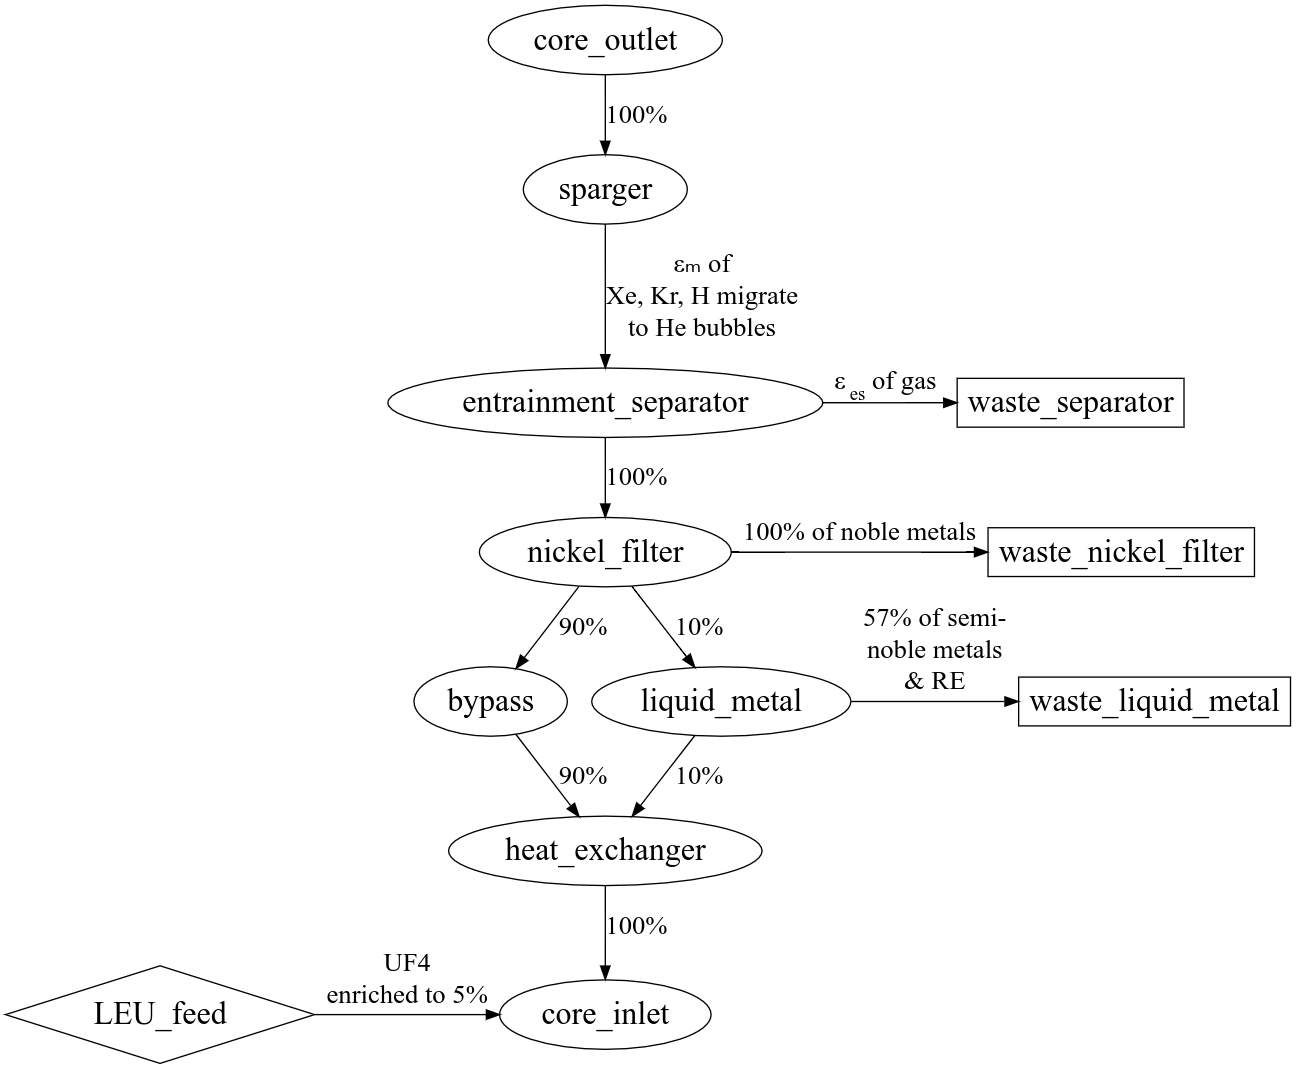
\includegraphics[width=\textwidth]{ch4/tap_saltproc_var_eps.png}
	\caption{\gls{TAP} reprocessing scheme flowchart used for the 
	demonstration of SaltProc v1.0.}
	\label{fig:demo-repro-scheme}
\end{figure}

Arrows on Figure~\ref{fig:demo-repro-scheme} represent material flows, 
percents 
represent a fraction of total mass flow rates; ellipses represent fuel 
reprocessing system components; boxes represent waste streams; the diamond 
shows refuel material flow (UF$_4$, 5 wt\% of $^{235}$U). The efficiency 
of gas migration to helium bubbles ($\epsilon_m$) and efficiency of 
gas bubbles separation from the salt ($\epsilon_{es}$) are different for 
various demonstration cases and discussed in more detail in 
Sections~\ref{sec:ben-valid} and \ref{sec:long-term-real}. Efficiency of 
noble metal extraction in the nickel filter 
(Figure~\ref{fig:tap-primary-scheme}, orange block) and semi-noble metals/rare 
earths (RE) in the liquid metal extraction system 
(Figure~\ref{fig:tap-primary-scheme}, green block) is assumed fixed and equal 
100\% and 57\%, respectively.

The gas removal components (sparger/contactor and entrainment separator) are 
located in-line because the estimated full loop time\footnote{Full loop time 
is the time taken by a particle of the coolant to make one full circle in the 
primary loop.} for the fuel salt is about 20 seconds and approximately equal 
to the cycle time (Table~\ref{tab:reprocessing_list}). To extract volatile 
gases every 20 seconds, the gas removal system must operate with 100\% of the 
core throughout flow rate (in-line gas removal system). In this chapter, the 
efficiency of noble gas migration to helium bubbles and the efficiency of 
bubble removal from the salt by the entrainment separator  
($\epsilon_m,\epsilon_{es}$ on Figure~\ref{fig:demo-repro-scheme},  
respectively) are selected separately for each demonstration case.

The nickel filter in the \gls{TAP} concept is designed to extract 
noble/semi-noble metals and volatile fluorides 
(Table~\ref{tab:reprocessing_list}). Similar to volatile gases, 
noble metals must be removed every 20 seconds and, hence, the filter should 
operate at 100\% of the flow rate through the core. The nickel filter removes 
a wide range of elements with various effective cycle time 
(Table~\ref{tab:reprocessing_list}).

Lanthanides and other non-noble metals have a lower capture cross section than 
gases and noble metals. These elements can be removed via a 
liquid-metal/molten salt extraction process with relatively low removal rates 
(cycle time $>50$ days). This is accomplished by directing a small fraction of 
the salt mass flow leaving the nickel mesh filter (10\% of the flow rate 
throughout the core) to the liquid-metal/molten salt component of the 
reprocessing system, in which lanthanides are removed with a specific 
extraction efficiency to match the  required cycle time  
(Table~\ref{tab:reprocessing_list}). The remaining 90\% of the salt mass flow 
is directed from the nickel filter to the heat exchangers without performing 
any fuel salt treatment.

The removal rates vary among nuclides in this reactor concept, which dictate 
the necessary resolution of depletion calculations. To compromise, a 3-day 
depletion time step was selected for the long-term demonstration case based on 
a time step refinement study by Betzler \emph{et al.} 
\cite{betzler_assessment_2017-1} A complimentary time step refinement study is
presented in Section~\ref{sec:time-refinement} to determine the impact of 
temporal resolution on the depleted composition calculation.

\section{Long-term depletion demonstration and validation}\label{sec:long-term}
\subsection{Constant, ideal extraction efficiency case}\label{sec:ben-valid}
To validate SaltProc v1.0, I performed a lifetime-long depletion calculation 
with ideal extraction efficiency. This case was selected to repeat fuel salt 
depletion as close as possible to the ChemTriton simulation for the full-core 
\gls{TAP} reactor by Betzler \emph{et al.} \cite{betzler_assessment_2017-1}  
Betzler \emph{et al.} made the following assumptions and approximations in 
their work \cite{betzler_assessment_2017-1}:
\begin{enumerate}[label=(\alph*), noitemsep, topsep=0pt]	
	\item Effective cycle times as prescribed by the Transatomic Power 
	Technical White Paper \cite{transatomic_power_corporation_technical_2016} 
	(Table~\ref{tab:reprocessing_list}) with \textbf{100\% noble 
	gas removal efficiency}; hence, $\epsilon_{es}$ and $\epsilon_m$ in the
	reprocessing model (Figure~\ref{fig:demo-repro-scheme}) are both set to 
	1.0.
	\item 5\% \gls{LEU} feed rate is equal to the rate of fission product 
	removal.
	\item 3-day depletion step.
	\item Quarter-core, 3-D model with vacuum boundary conditions.
	\item Delayed neutron precursor drift was neglected.
\end{enumerate}

I adopted these assumptions for code-to-code verification of SaltProc v1.0 
against ChemTriton. The ENDF/B-VII.1 \cite{chadwick_endf/b-vii.1_2011} nuclear 
data library is used for this case to be consistent with Betzler's work.
Unfortunately, some crucial details have not been reported in 
\cite{betzler_assessment_2017-1}: (1) exact core geometries for various 
moderator rod configurations except startup configuration; (2) the excess 
reactivity at startup; (3) the library from which S($\alpha, \beta$) tables 
for thermal scattering in zirconium hydride are obtained. This section 
presented my best effort to repeat Betzler's simulation using the same input 
data to validate SaltProc for the \gls{TAP} concept.


\subsubsection{Effective multiplication factor dynamics}
Figures~\ref{fig:keff-ben-valid} and \ref{fig:keff-ben-valid-zoomed} 
demonstrate the effective multiplication factor obtained using SaltProc v1.0 
with Serpent. The $k_{eff}$ was obtained after removing fission products and 
adding feed material at the end of each depletion step (3 days for this case). 
SaltProc v1.0 updated the moderator rod configuration to the next 
configuration (e.g., from 1388 rods per core to 1624 rods per core) once the
predicted value of $k_{eff}$ at the end of the next depletion step dropped 
below 1. 
This algorithm mimics regular maintenance shutdown when the \gls{TAP} core 
excess reactivity is exhausted, and moderator rod assemblies should be 
reconfigured to operate the next cycle. 

An optimal number of moderator configurations (cycles) is found to be 15 (see 
Appendix~A). Fewer cycles would improve capacity factor 
but need larger excess reactivity at the \gls{BOC}, which is strictly limited 
by reactivity control system worth. More cycles would require more frequent 
moderator rod reconfigurations, which worsens the capacity factor.  The 
interval between the first and second moderator configuration was only 12 
months, the shortest interval between moderator configuration updates. For the 
operation interval between 2 and 16 years after startup, the intervals between 
shutdowns for moderator rod updates were 18-26 months. However, towards the 
\gls{EOL}, the intervals between moderator rod reconfigurations dropped to 13 
months. 
Overall, the average interval between regular shutdowns for the core 
reconfiguration was 18 months, which exactly matches the refueling interval 
for conventional \glspl{LWR} and is consistent with Betzler \emph{et al.} 
($\approx$16 months) \cite{betzler_assessment_2017-1}.
\begin{figure}[htp!] % replace 't' with 'b' to 
	\centering
	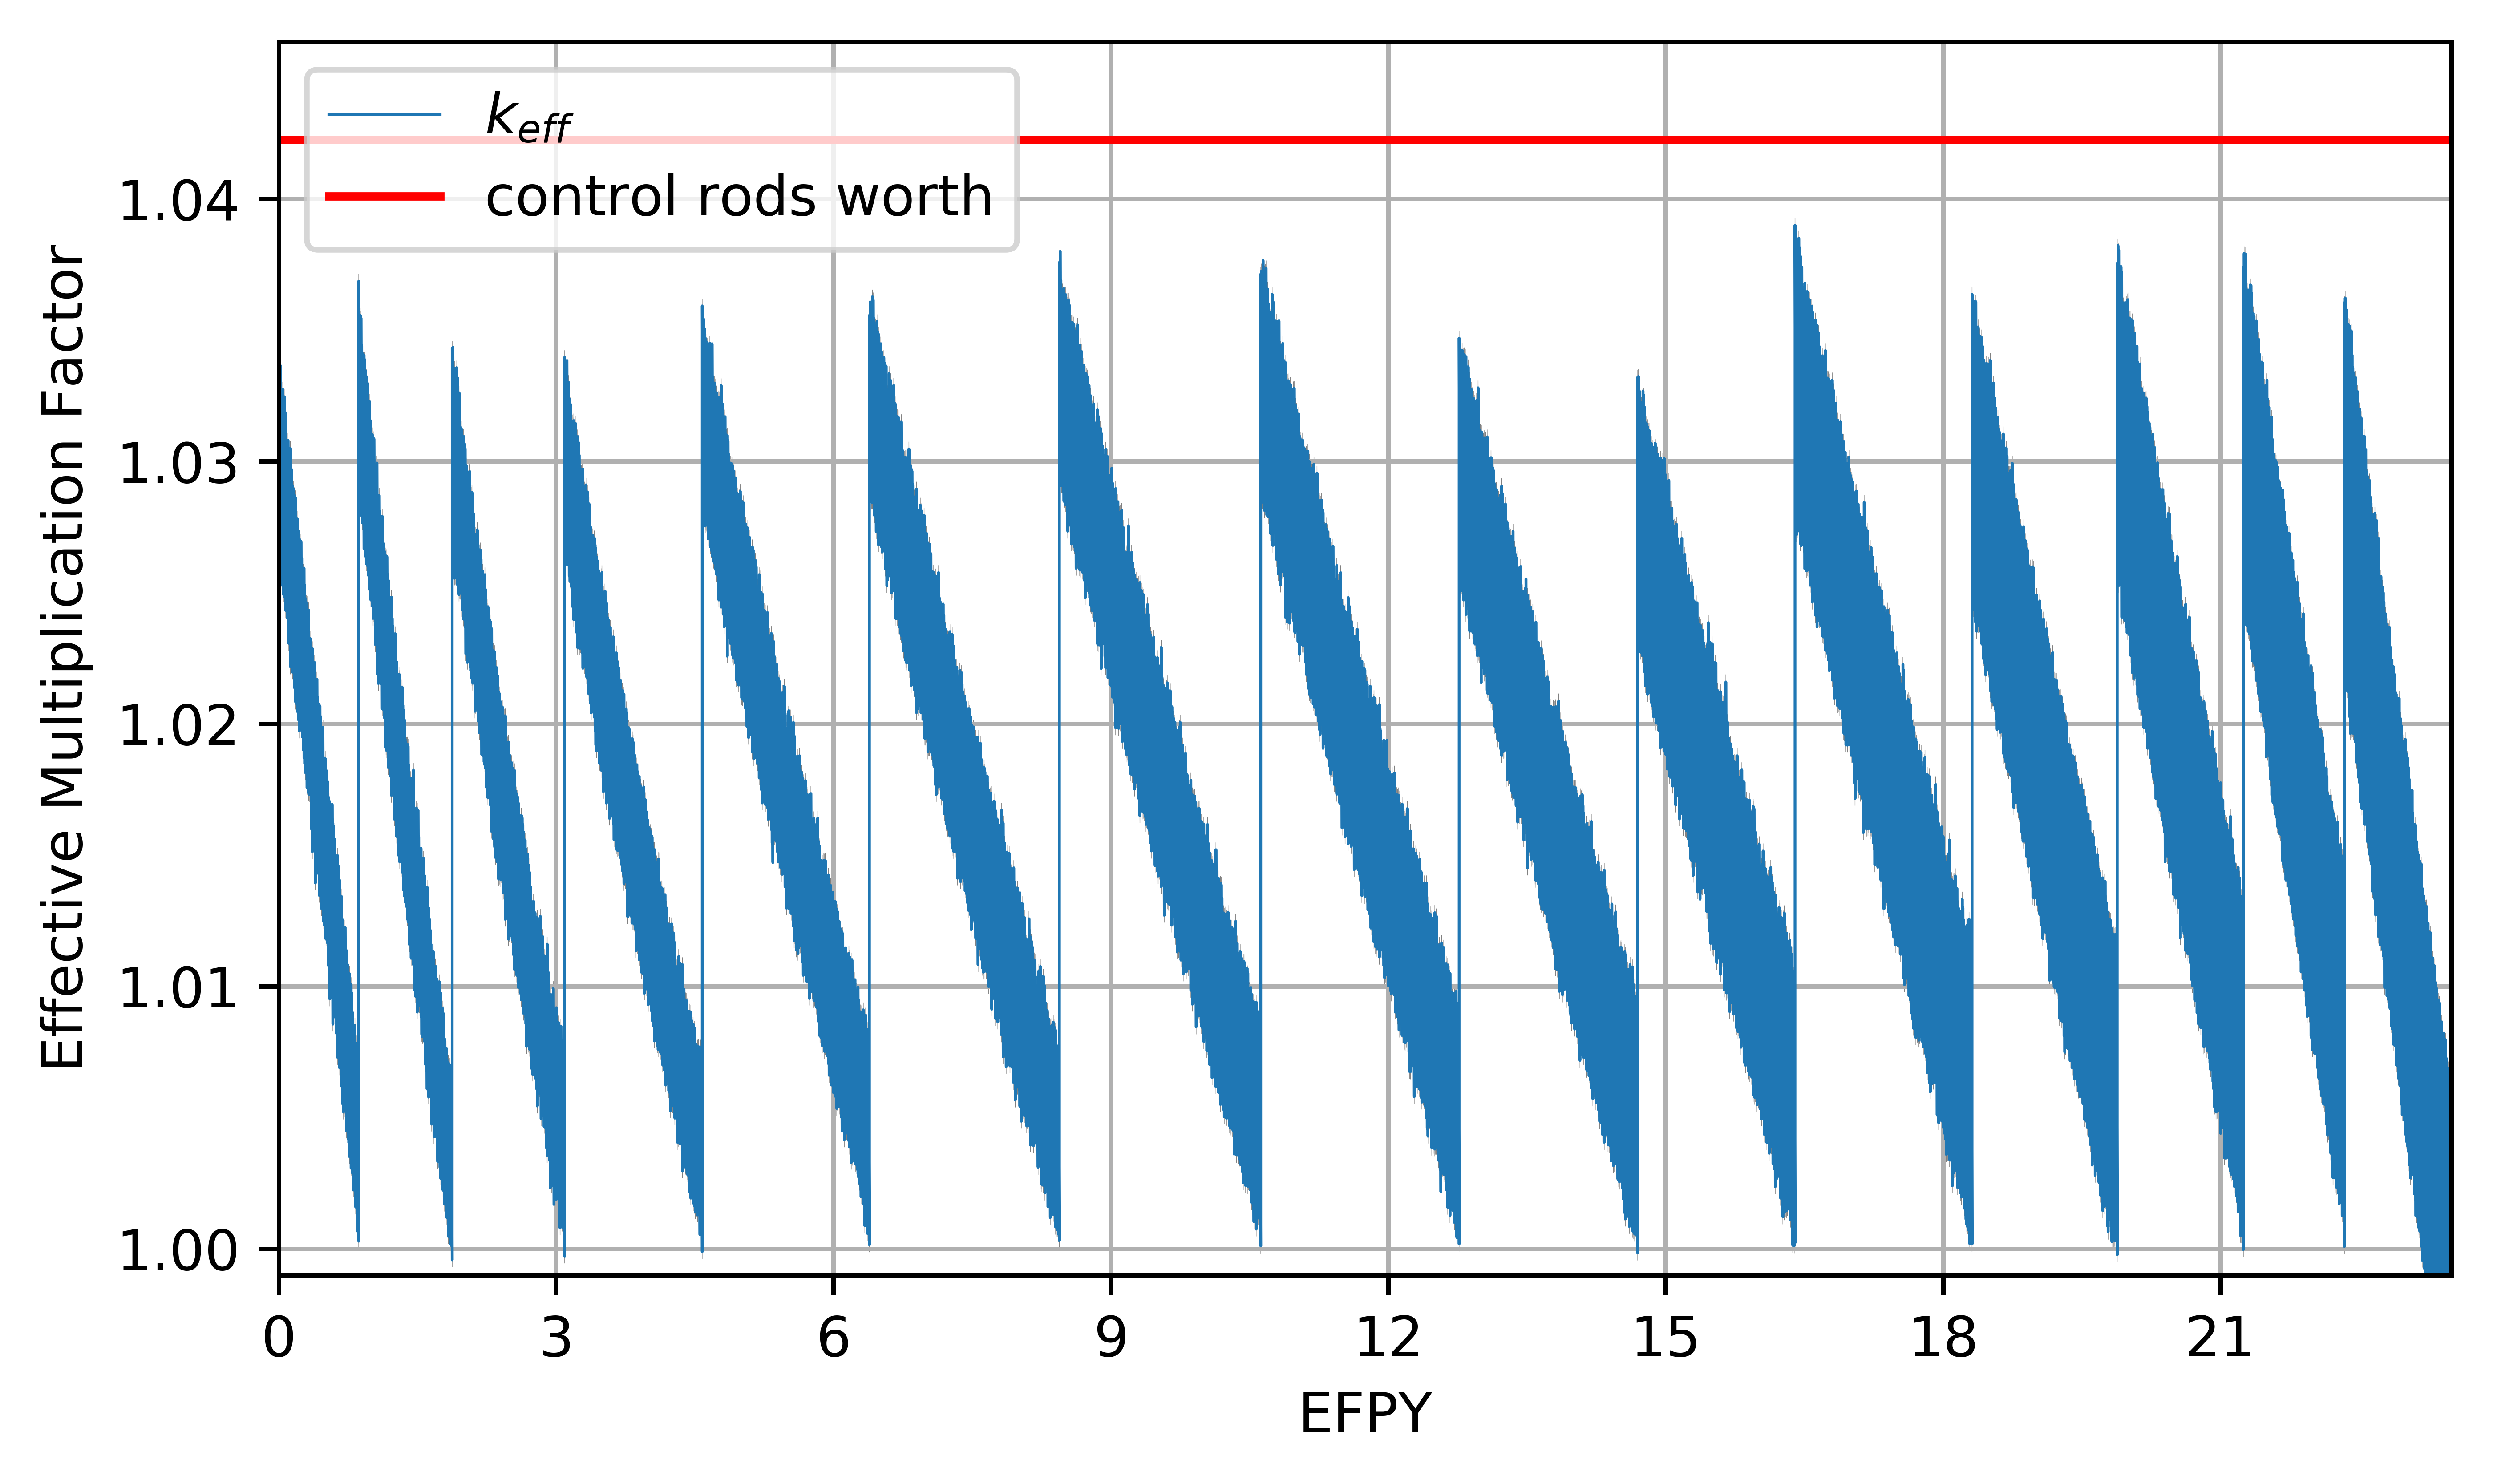
\includegraphics[width=\textwidth]{ch4/keff_ben.png}
		\vspace{-9mm}
	\caption{Effective multiplication factor dynamics during 23.5 years of 
	operation for the full-core \gls{TAP} core model for the case with an 
	ideal removal efficiency of fission product. Confidence interval 
	$\sigma=28$ $pcm$ is shaded.}
	\label{fig:keff-ben-valid}
\end{figure}
\begin{figure}[htp!] % replace 't' with 'b' to 
	\centering
	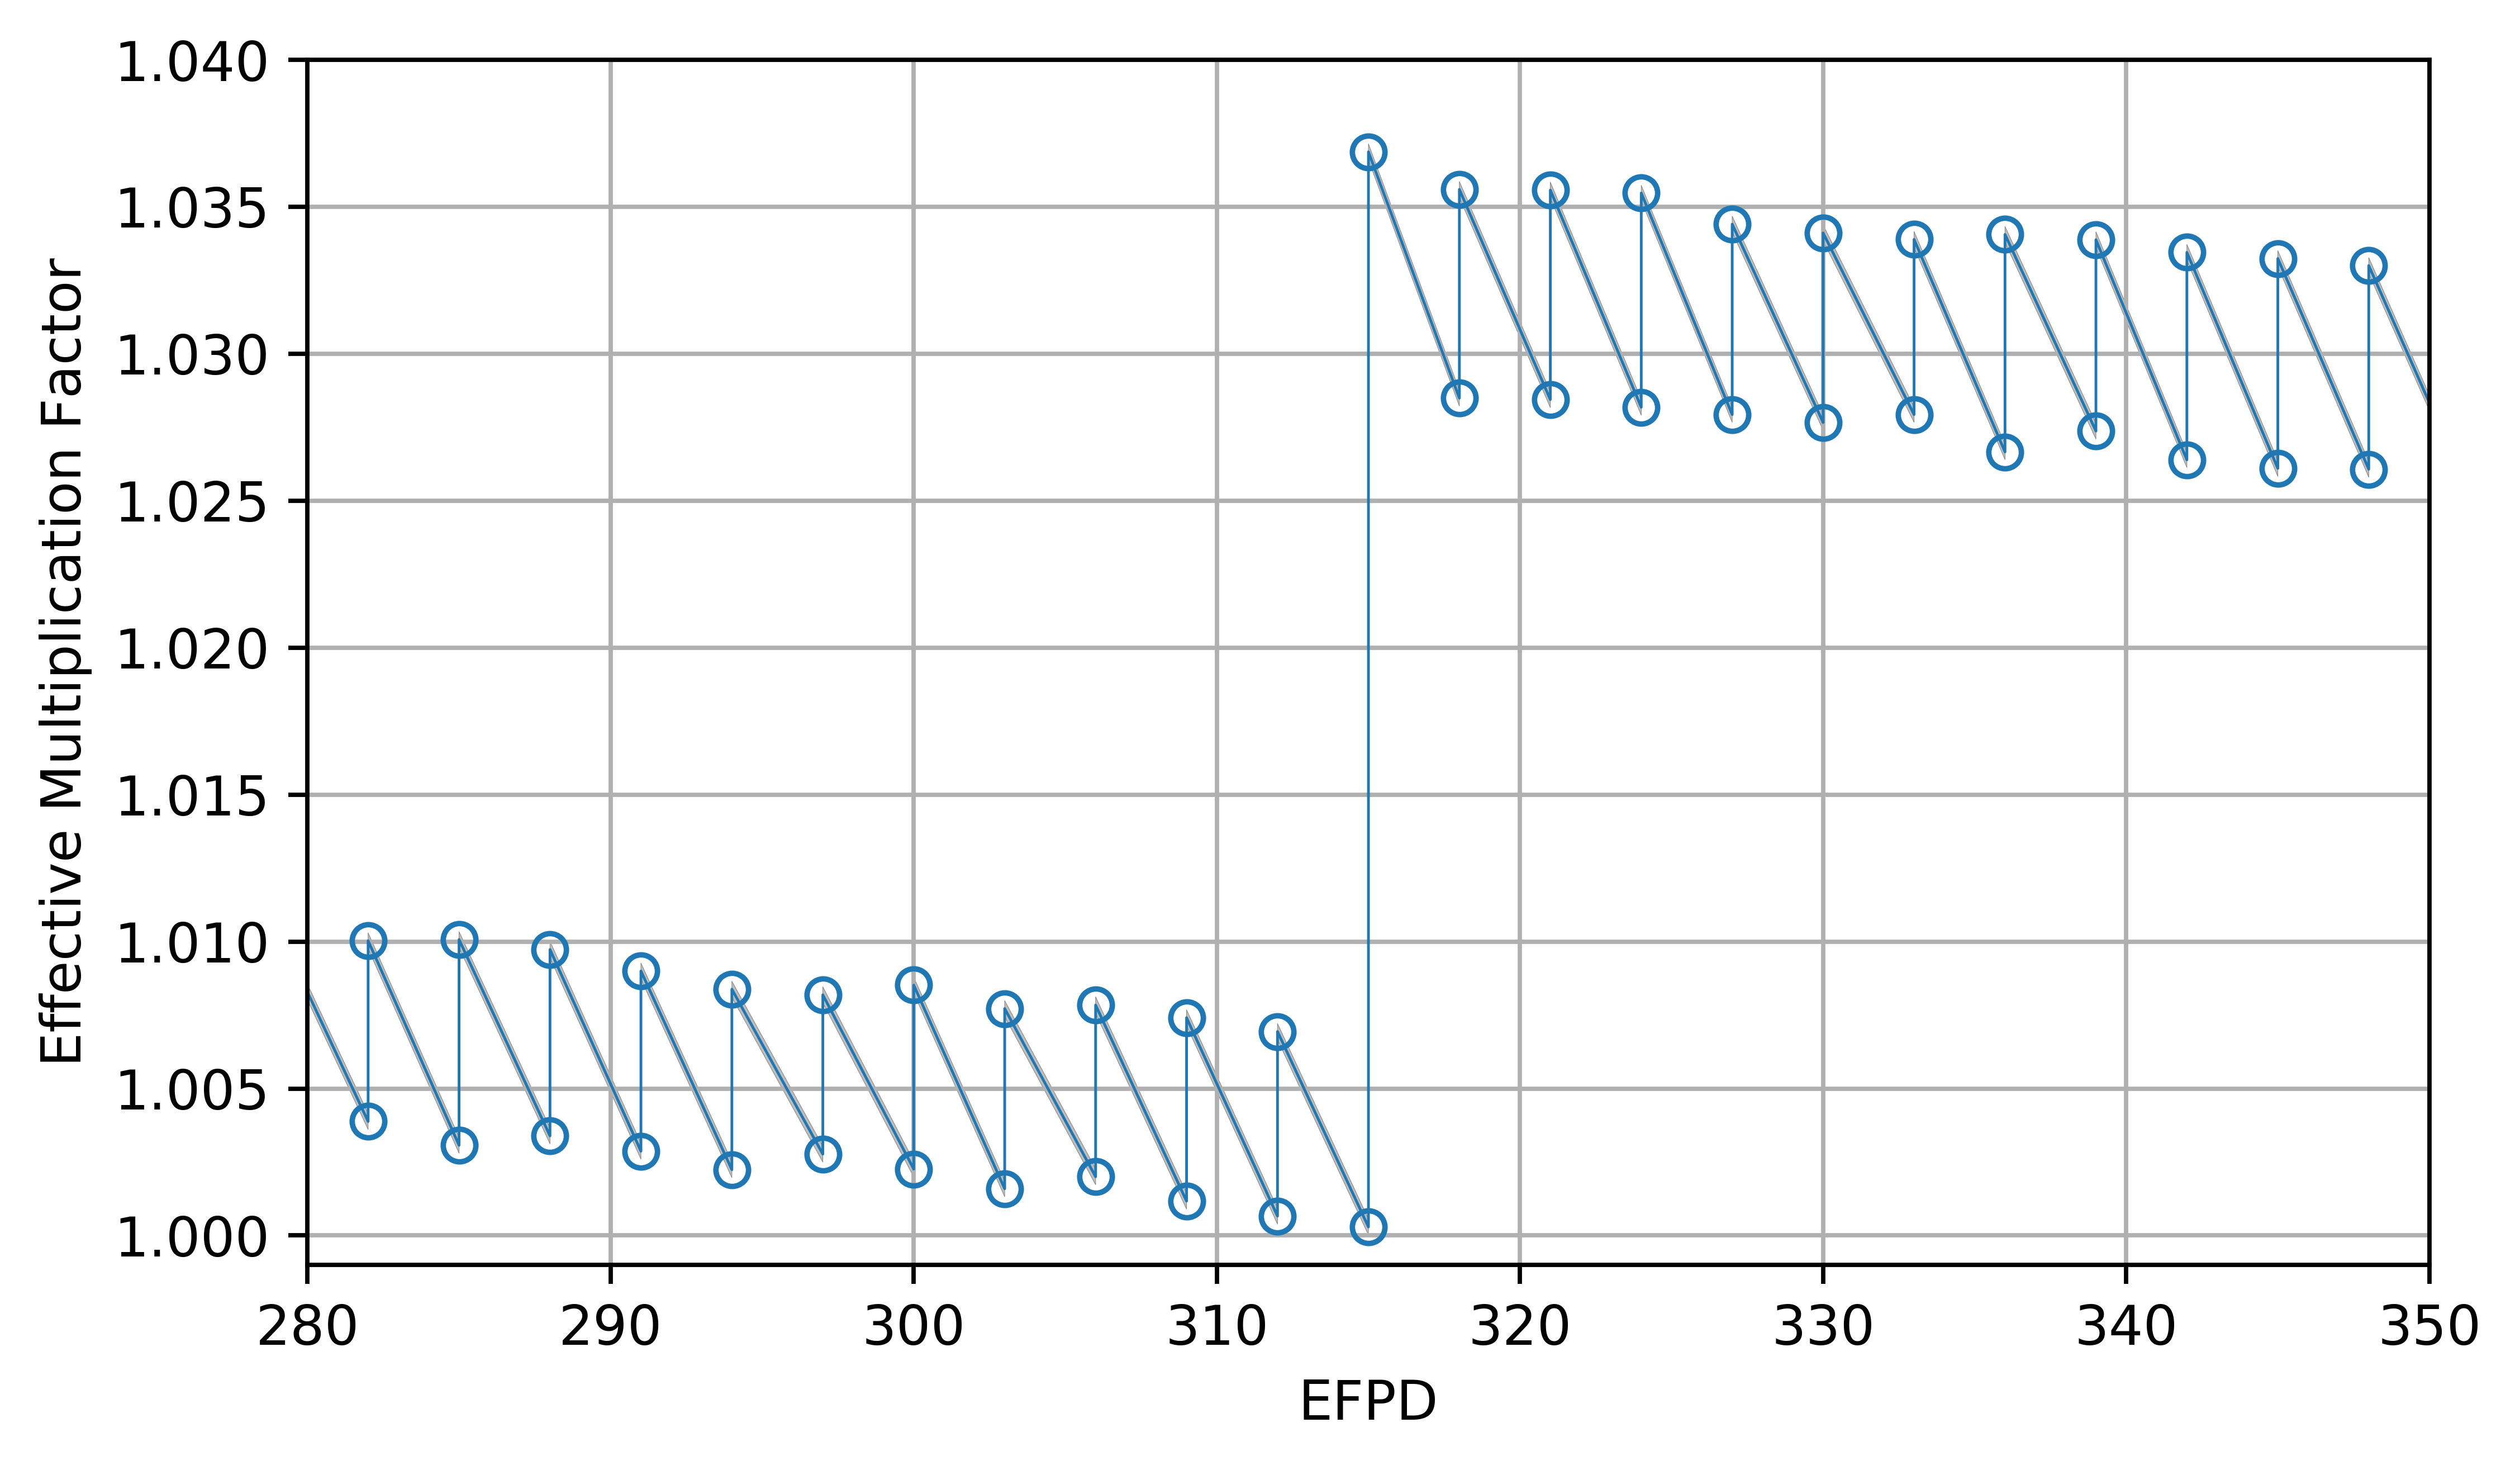
\includegraphics[width=0.93\textwidth]{ch4/keff_ben_zoomed.png}
		\vspace{-4mm}
	\caption{Zoomed effective multiplication factor for the interval from 280 
		to 350 EFPD while transitioning from Cycle \#1 (startup geometry 
		configuration, 347 moderator rods, \gls{SVF}=0.91720353) to Cycle \#2 
		(\gls{SVF}=0.88694). Confidence interval $\sigma=28$ $pcm$ is 
		shaded.}
	\label{fig:keff-ben-valid-zoomed}
\end{figure}

The $k_{eff}$ fluctuates significantly as a result of the batch-wise nature of 
the online reprocessing approach used. Loading the initial fuel salt 
composition with 5\% \gls{LEU} into the \gls{TAP} core leads to a 
supercritical configuration with an excess reactivity of about 3200 $pcm$
(Figure~\ref{fig:keff-ben-valid}). Without performing any fuel salt 
reprocessing and spectrum shifting, the core became subcritical after 30 days 
of operation \cite{rykhlevskii_milestone_2019}. SaltProc calculates an 
operational lifetime of 22.5 years, after which the fuel salt reached a total 
burnup of 81.46 MWd/kgU. The end of an operational lifetime is achieved when 
the minimum \gls{SVF} is obtained, as restricted by the moderator geometry 
parameters (e.g., moderator rod diameter, rod pitch, the internal diameter of 
the reactor vessel). Table~\ref{tab:valid_ben_lifetime} compares obtained 
results with Betzler \emph{et al.} \cite{betzler_assessment_2017-1}. Overall, 
SaltProc-calculated operational lifetime and burnup are lower than the 
reference by approximately 22\% and 17\%, respectively. A better match in the 
operational lifetime between SaltProc v1.0 and ChemTriton can be obtained if a
detailed moderator configuration description of Betzler's model will be 
available in the future.

%%%%%%%%%%%%%%%%%%%%%%%%%%%%%%%%%%%%%%%%
\begin{table}[htp!]
	\centering
	\caption{Comparison of main operational parameters in the \gls{TAP} 
	reactor between the current work and Betzler \emph{et al.}
	\cite{betzler_assessment_2017-1}.}
	\begin{tabularx}{\textwidth}{p{0.42\textwidth} R R}
		\hline
		\textbf{Parameter}  & \textbf{Current work} & \textbf{Betzler, 2017} 
		\cite{betzler_assessment_2017-1}\\ \hline
		Operational lifetime [y] & 22.5 & 29.0 \\
		Discharge burnup [MWd/kgU] & 76.30& 91.9 \\
		Average moderator reconfiguration interval [months] & 18 & 16 \\
		\hline
	\end{tabularx}
	\label{tab:valid_ben_lifetime}
\end{table}
%%%%%%%%%%%%%%%%%%%%%%%%%%%%%%%%%%%%%%%%%%%%%%%%%%%%%%%%%%%%%%%%%%%%%%%%%%%%%%%

\subsubsection{Fuel salt isotopic composition dynamics}
Figure~\ref{fig:u-ben-valid} show that continuous \gls{LEU} feed into the 
\gls{TAP} reactor is not sufficient to maintain the fissile $^{235}$U content 
of the core, as the uranium enrichment steadily decreases from 5\% at the 
\gls{BOL} to 1\% at the \gls{EOL}. However, during the first 13 years of 
operation, the \gls{TAP} \gls{MSR} breeds fissile $^{239}$Pu and $^{241}$Pu, 
reaching a peak of total fissile plutonium inventory of 2.15 t  
(Figure~\ref{fig:pu-fiss-ben-valid}). Figure~\ref{fig:pu-ben-valid} shows that
a significant amount of non-fissile 
plutonium ($^{238}$Pu, $^{240}$Pu, and $^{242}$Pu) and uranium ($^{236}$U) 
builds up in the reactor during operation and negatively impacts criticality 
of the reactor. $^{239}$Pu and $^{241}$Pu are major contributors to the 
fissile material content of the core, keeping it critical during the second 
half of the operational lifecycle. The total $^{239}$Pu inventory in the core 
rises during the first 11 years of operation due to the harder neutron 
spectrum. After 11 years, the softer spectrum breeds less $^{239}$Pu from 
$^{238}$U, and more of $^{239}$Pu is progressively burned. Obtained results 
are in good agreement with results in ORNL Report by Betzler \emph{et al.} 
(Table~\ref{tab:valid_ben_isos}) \cite{betzler_assessment_2017-1}.

%$^{235}$U inventory in Betzler \emph{et al.} changed from 6.8t at the 
%\gls{BOL} to 1.0t at the \gls{EOL}. $^{239}$Pu  was 1.065t at the 
%\gls{EOL}. $^{240}$Pu  was 995kg at the 
%\gls{EOL}. $^{241}$Pu  was 465kg at the 
%\gls{EOL}.		
\begin{figure}[htp!] % replace 't' with 'b' to 
	\centering
	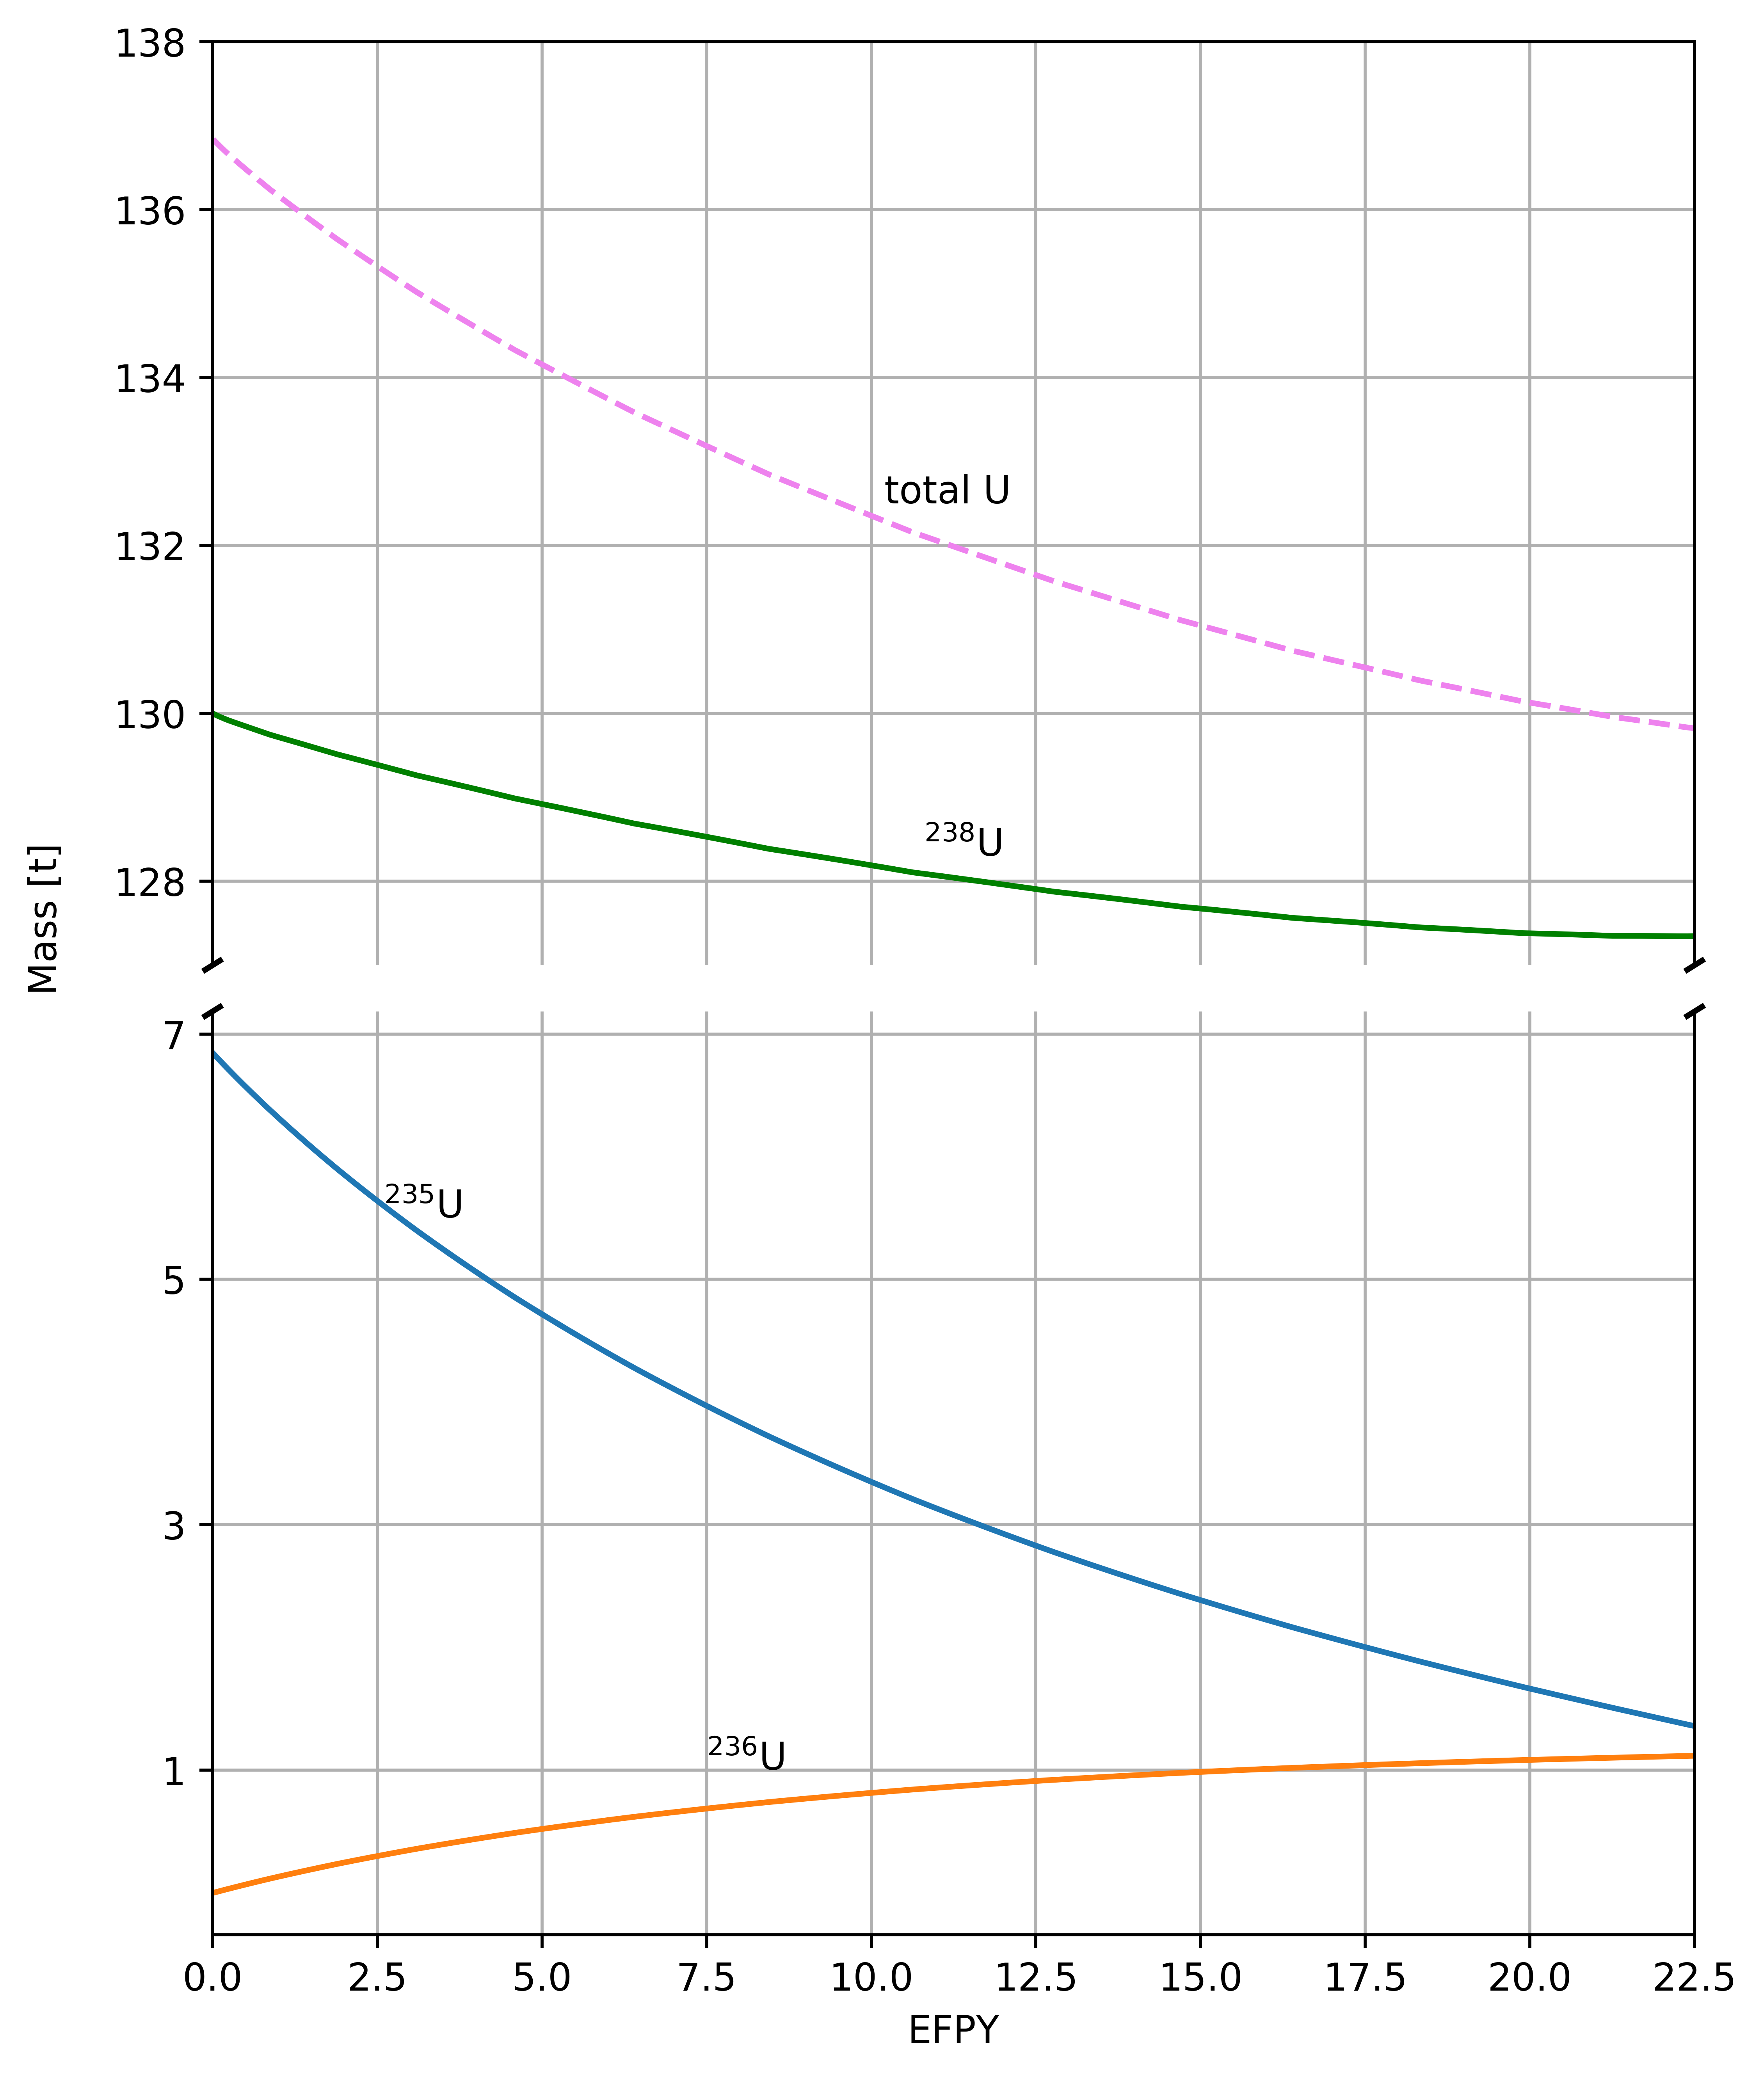
\includegraphics[width=\textwidth]{ch4/u_ben_valid.png}
	\caption{SaltProc-calculated uranium isotopic fuel salt content during 
	22.5 years of operation. Uncertainty of the predicted mass will be 
	estimated and discussed in Chapter~\ref{ch:uq}.}
	\label{fig:u-ben-valid}
\end{figure}

\begin{figure}[htp!] % replace 't' with 'b' to 
	\centering
	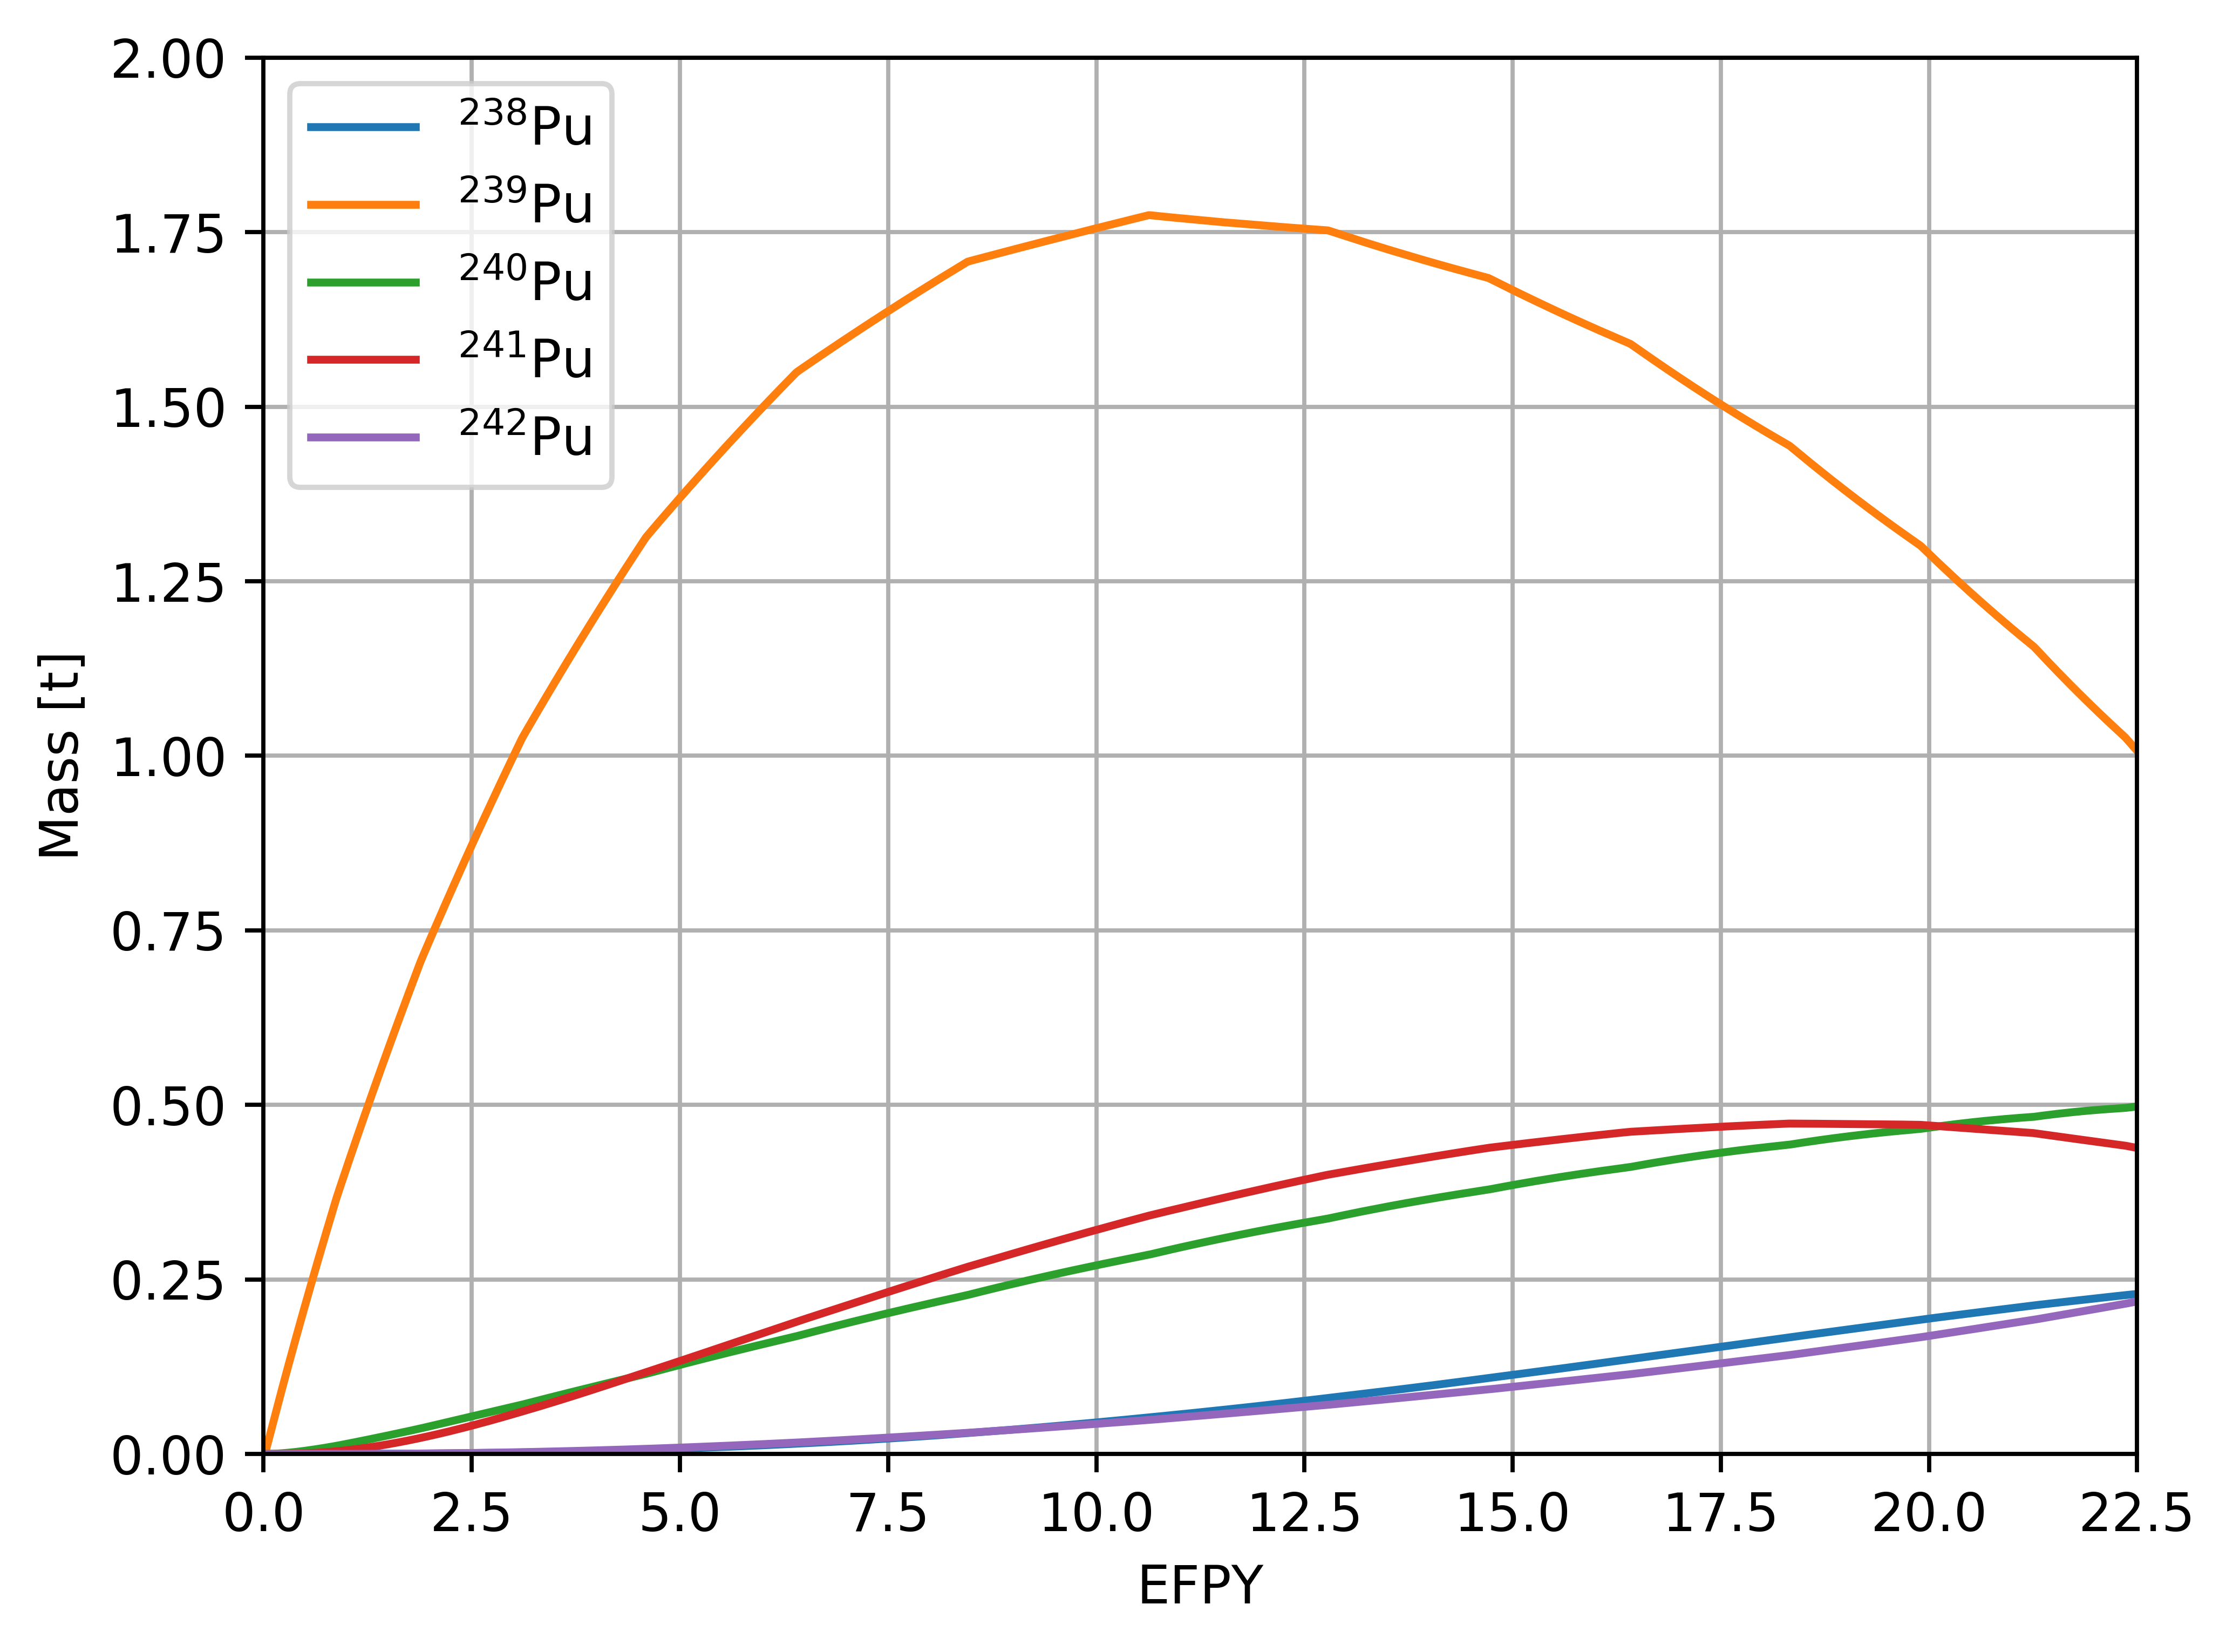
\includegraphics[width=0.83\textwidth]{ch4/pu_ben_valid.png}
		\vspace{-4mm}
	\caption{SaltProc-calculated plutonium isotopic fuel salt content during 
		22.5 years of operation.}
	\label{fig:pu-ben-valid}
\end{figure}
\begin{figure}[hbp!] % replace 't' with 'b' to 
	\centering
	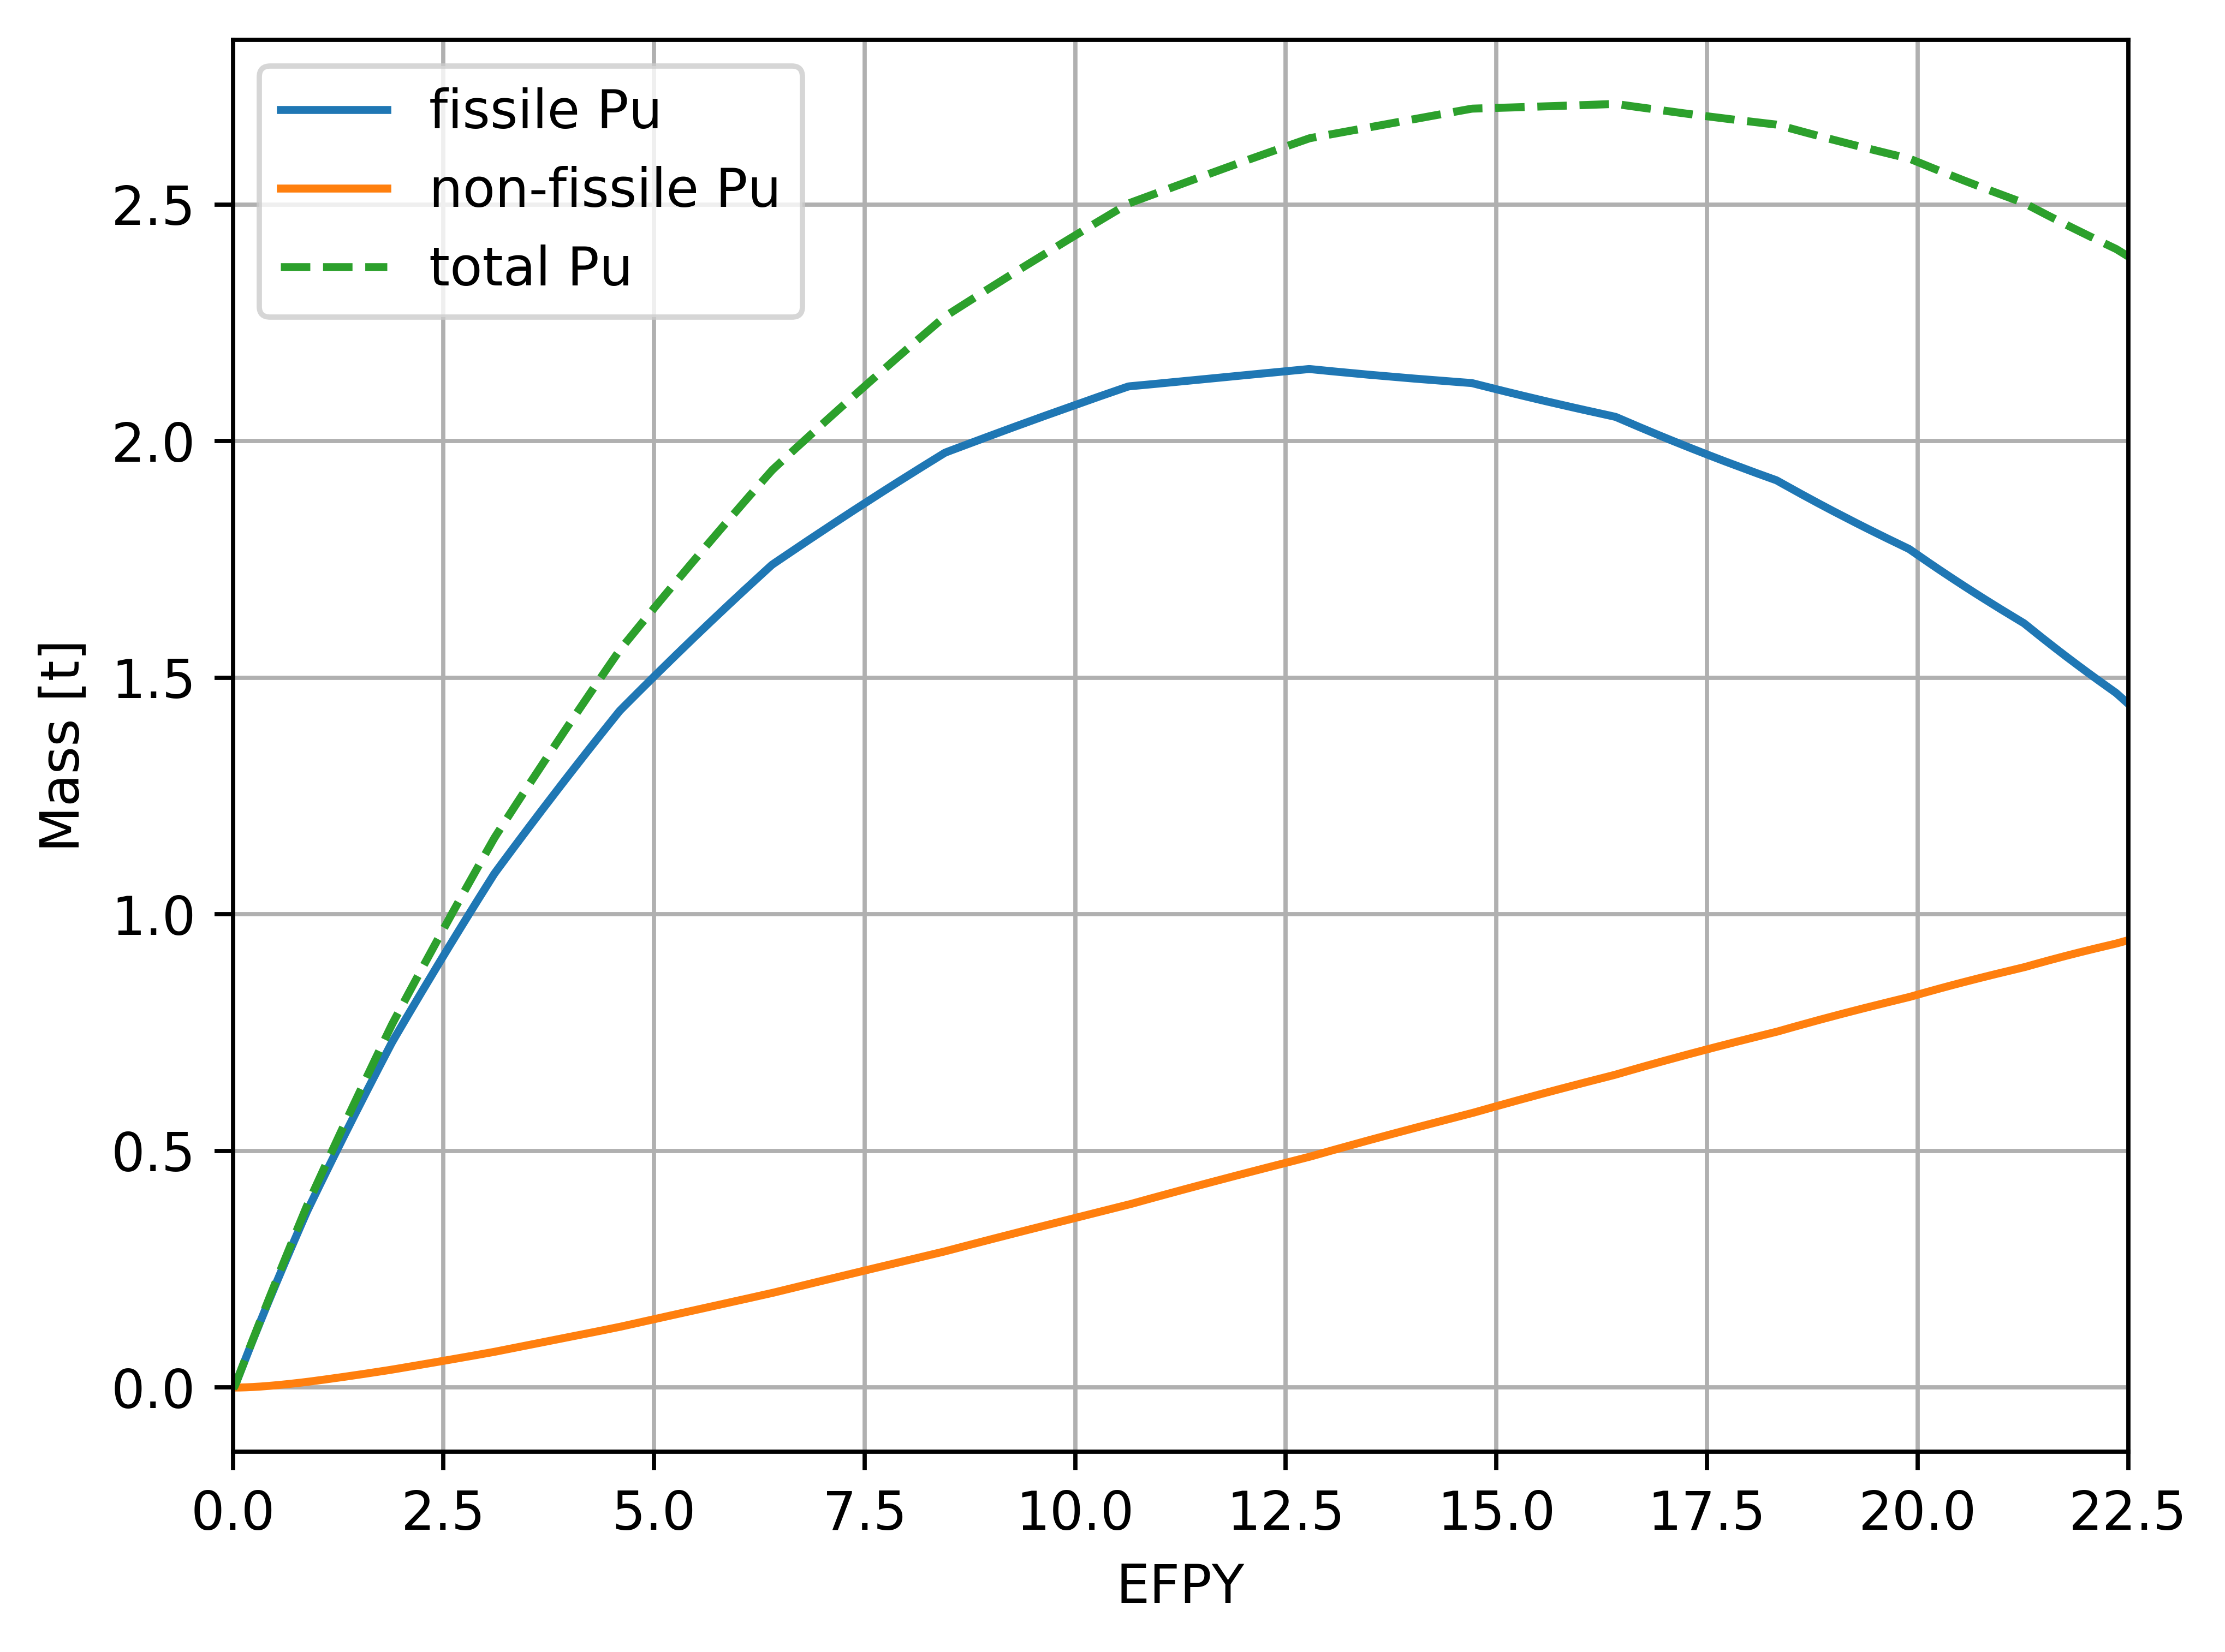
\includegraphics[width=0.83\textwidth]{ch4/tot_pu_ben_valid.png}
		\vspace{-4mm}
	\caption{SaltProc-calculated fissile and non-fissile plutonium fuel salt 
	content during 22.5 years of operation.}
	\label{fig:pu-fiss-ben-valid}
\end{figure}

%%%%%%%%%%%%%%%%%%%%%%%%%%%%%%%%%%%%%%%%
\begin{table}[htp!]
	\centering
	\caption{Comparison of major heavy isotopes inventories at the \gls{EOL} 
	in the \gls{TAP} reactor between the current work and Betzler \emph{et al.}	
	\cite{betzler_assessment_2017-1}.}
	\begin{tabularx}{\textwidth}{L p{0.12\textwidth} R R R}
		\hline
		& \textbf{Isotope}  & \textbf{Current work mass [kg]} & 
		\textbf{Betzler, 2017 mass [kg]} & \textbf{$\Delta m$ [\%]}\\ \hline
		\multirow{4}{*}{Fissile}
		&$^{235}$U  & 1299 & 1160 & $+11$\% \\
		&$^{239}$Pu & 942  & 995  & $-5$\% \\
		&$^{241}$Pu & 427  & 435  & $-2$\% \\
		&Total & 2668 & 2590 & $+3$\%  \\ \hline
		
		\multirow{4}{*}{Non-fissile}
		&$^{236}$U  & 1123 & 1200 & $-6$\% \\
		&$^{238}$U  & 127,353 & 132,400 & $-4$\% \\
		&$^{238}$Pu & 235  & 280  & $-16$\% \\
		&$^{240}$Pu & 503  & 1000  & $-50$\% \\
		&$^{242}$Pu & 230  & 310  & $-26$\% \\
		&Total & 129,444 & 135,190 & $+4$\%  \\ \hline
	\end{tabularx}
	\label{tab:valid_ben_isos}
	\vspace{-0.9em}
\end{table}
%%%%%%%%%%%%%%%%%%%%%%%%%%%%%%%%%%%%%%%%%%%%%%%%%%%%%%%%%%%%%%%%%%%%%%%%%%%%%%%

A lifetime-long SaltProc depletion calculation requires a 5\% \gls{LEU} feed 
rate of 460.8 
kg per year to maintain the fuel salt inventory in the primary loop, which is 
consistent with the reference. Table~\ref{tab:valid_ben_performance} shows the
main fuel cycle performance parameters calculated using SaltProc and compared 
with the reference. Normalized per GW$_{th}$-year, the \gls{TAP} concept 
requires about 5.23 t of fuel compared with 4.14 t reported by Betzler 
\emph{et al.} SaltProc-calculated waste production normalized per 
GW$_{th}$-year is 5\% less than reported by ORNL. Potentially, the \gls{TAP} 
can operate with \gls{LWR} \gls{SNF} as the fissile material feed. The heavy 
metal component of \gls{LWR} \gls{SNF} has a lower fissile material weight 
fraction than 5\% enriched uranium and adds less fertile $^{238}$U to the fuel 
salt, potentially reducing the operational lifetime. Nevertheless, in the case 
of using waste material (e.g., transuranium elements from \gls{LWR} \gls{SNF}) 
in this fueling scenario, the \gls{TAP} concept has superior waste reduction 
metrics.
%%%%%%%%%%%%%%%%%%%%%%%%%%%%%%%%%%%%%%%%
\begin{table}[hbp!]
	\centering
	\caption{Comparison of normalized by GW$_{th}$-year total fuel load and 
	actinide waste from the TAP reactor obtained in the current work and 
	Betzler \emph{et al.} 
	\cite{betzler_assessment_2017-1}.}
	\begin{tabularx}{\textwidth}{p{0.42\textwidth} R R}
		\hline
		\textbf{Parameter}  & \textbf{Current work} & \textbf{Betzler, 2017} 
		\cite{betzler_assessment_2017-1}\\ \hline
		5\% \gls{LEU} feed rate [kg/y] & 460.8 & 480.0 \\
		Loaded fuel [t per GW$_{th}$-y] & 5.23 & 4.14 \\
		Waste  [t per GW$_{th}$-y] & 3.57 & 3.74 \\
		\hline
	\end{tabularx}
	\label{tab:valid_ben_performance}
	\vspace{-0.9em}
\end{table}
%%%%%%%%%%%%%%%%%%%%%%%%%%%%%%%%%%%%%%%%%%%%%%%%%%%%%%%%%%%%%%%%%%%%%%%%%%%%%%%

\newpage
\subsubsection{Neutron energy spectrum}
Significant thermalization of the neutron spectrum is observed as moderator 
rods are added into the core configuration 
(Figure~\ref{fig:ben-spectrum-bol}). At startup, the neutron spectra from the 
current work and Betzler \emph{et al.} are matched well because the core 
geometry, its \gls{SVF}, and initial fuel composition in these two simulations 
are similar. The Pearson correlation coefficient\footnote{Pearson correlation 
coefficient is calculated by the following formula:
	\begin{align}
	r &= \frac{\sum_{i=1}^{N} 
		(\Phi_i^{ref}-\overline{\Phi^{ref}})(\Phi_i-\overline{\Phi})}
	{\sqrt{\sum_{i=1}^{N} (\Phi_i^{ref}-\overline{\Phi^{ref}})^2 
			\sum_{i=1}^{N} 
			(\Phi_i-\overline{\Phi})^2}}\\
	\mbox{where} \nonumber\\
	\Phi_i^{ref},\Phi_i &= \mbox{neutron flux for i$^{th}$ energy bin 
		reported in the reference and the current work $[n/cm^2\cdot s]$} 
	\nonumber\\
	\overline{\Phi^{ref}}, \overline{\Phi} &= \mbox{neutron flux averaged over 
		N energy bins reported in the reference and current work $[n/cm^2\cdot 
		s]$} 
	\nonumber\\
	N &= \mbox{number of neutron energy bins [-].}
	\nonumber
	\end{align}}
$r_{BOL}=0.91115$, which indicates a strong, positive association between the 
spectra at the \gls{BOL} (see Figure~\ref{fig:ben-spectrum-bol}, upper plot).
At the \gls{EOL}, SaltProc/Serpent-calculated spectrum is more thermal than 
reported by Betzler \emph{et al.} \cite{betzler_assessment_2017-1}, but the
correlation coefficient $r_{EOL}=0.90987$ shows that the spectra are still 
extremely strongly related (see Figure~\ref{fig:ben-spectrum-bol}, lower 
plot). 
%with smaller amplitude of resonances between 10$^{-5}$ and 10$^{-2}$ MeV 
%(resonance capture of neutrons by $^{238}$U).
\begin{figure}[htbp!] % replace 't' with 'b' to 
	\centering
	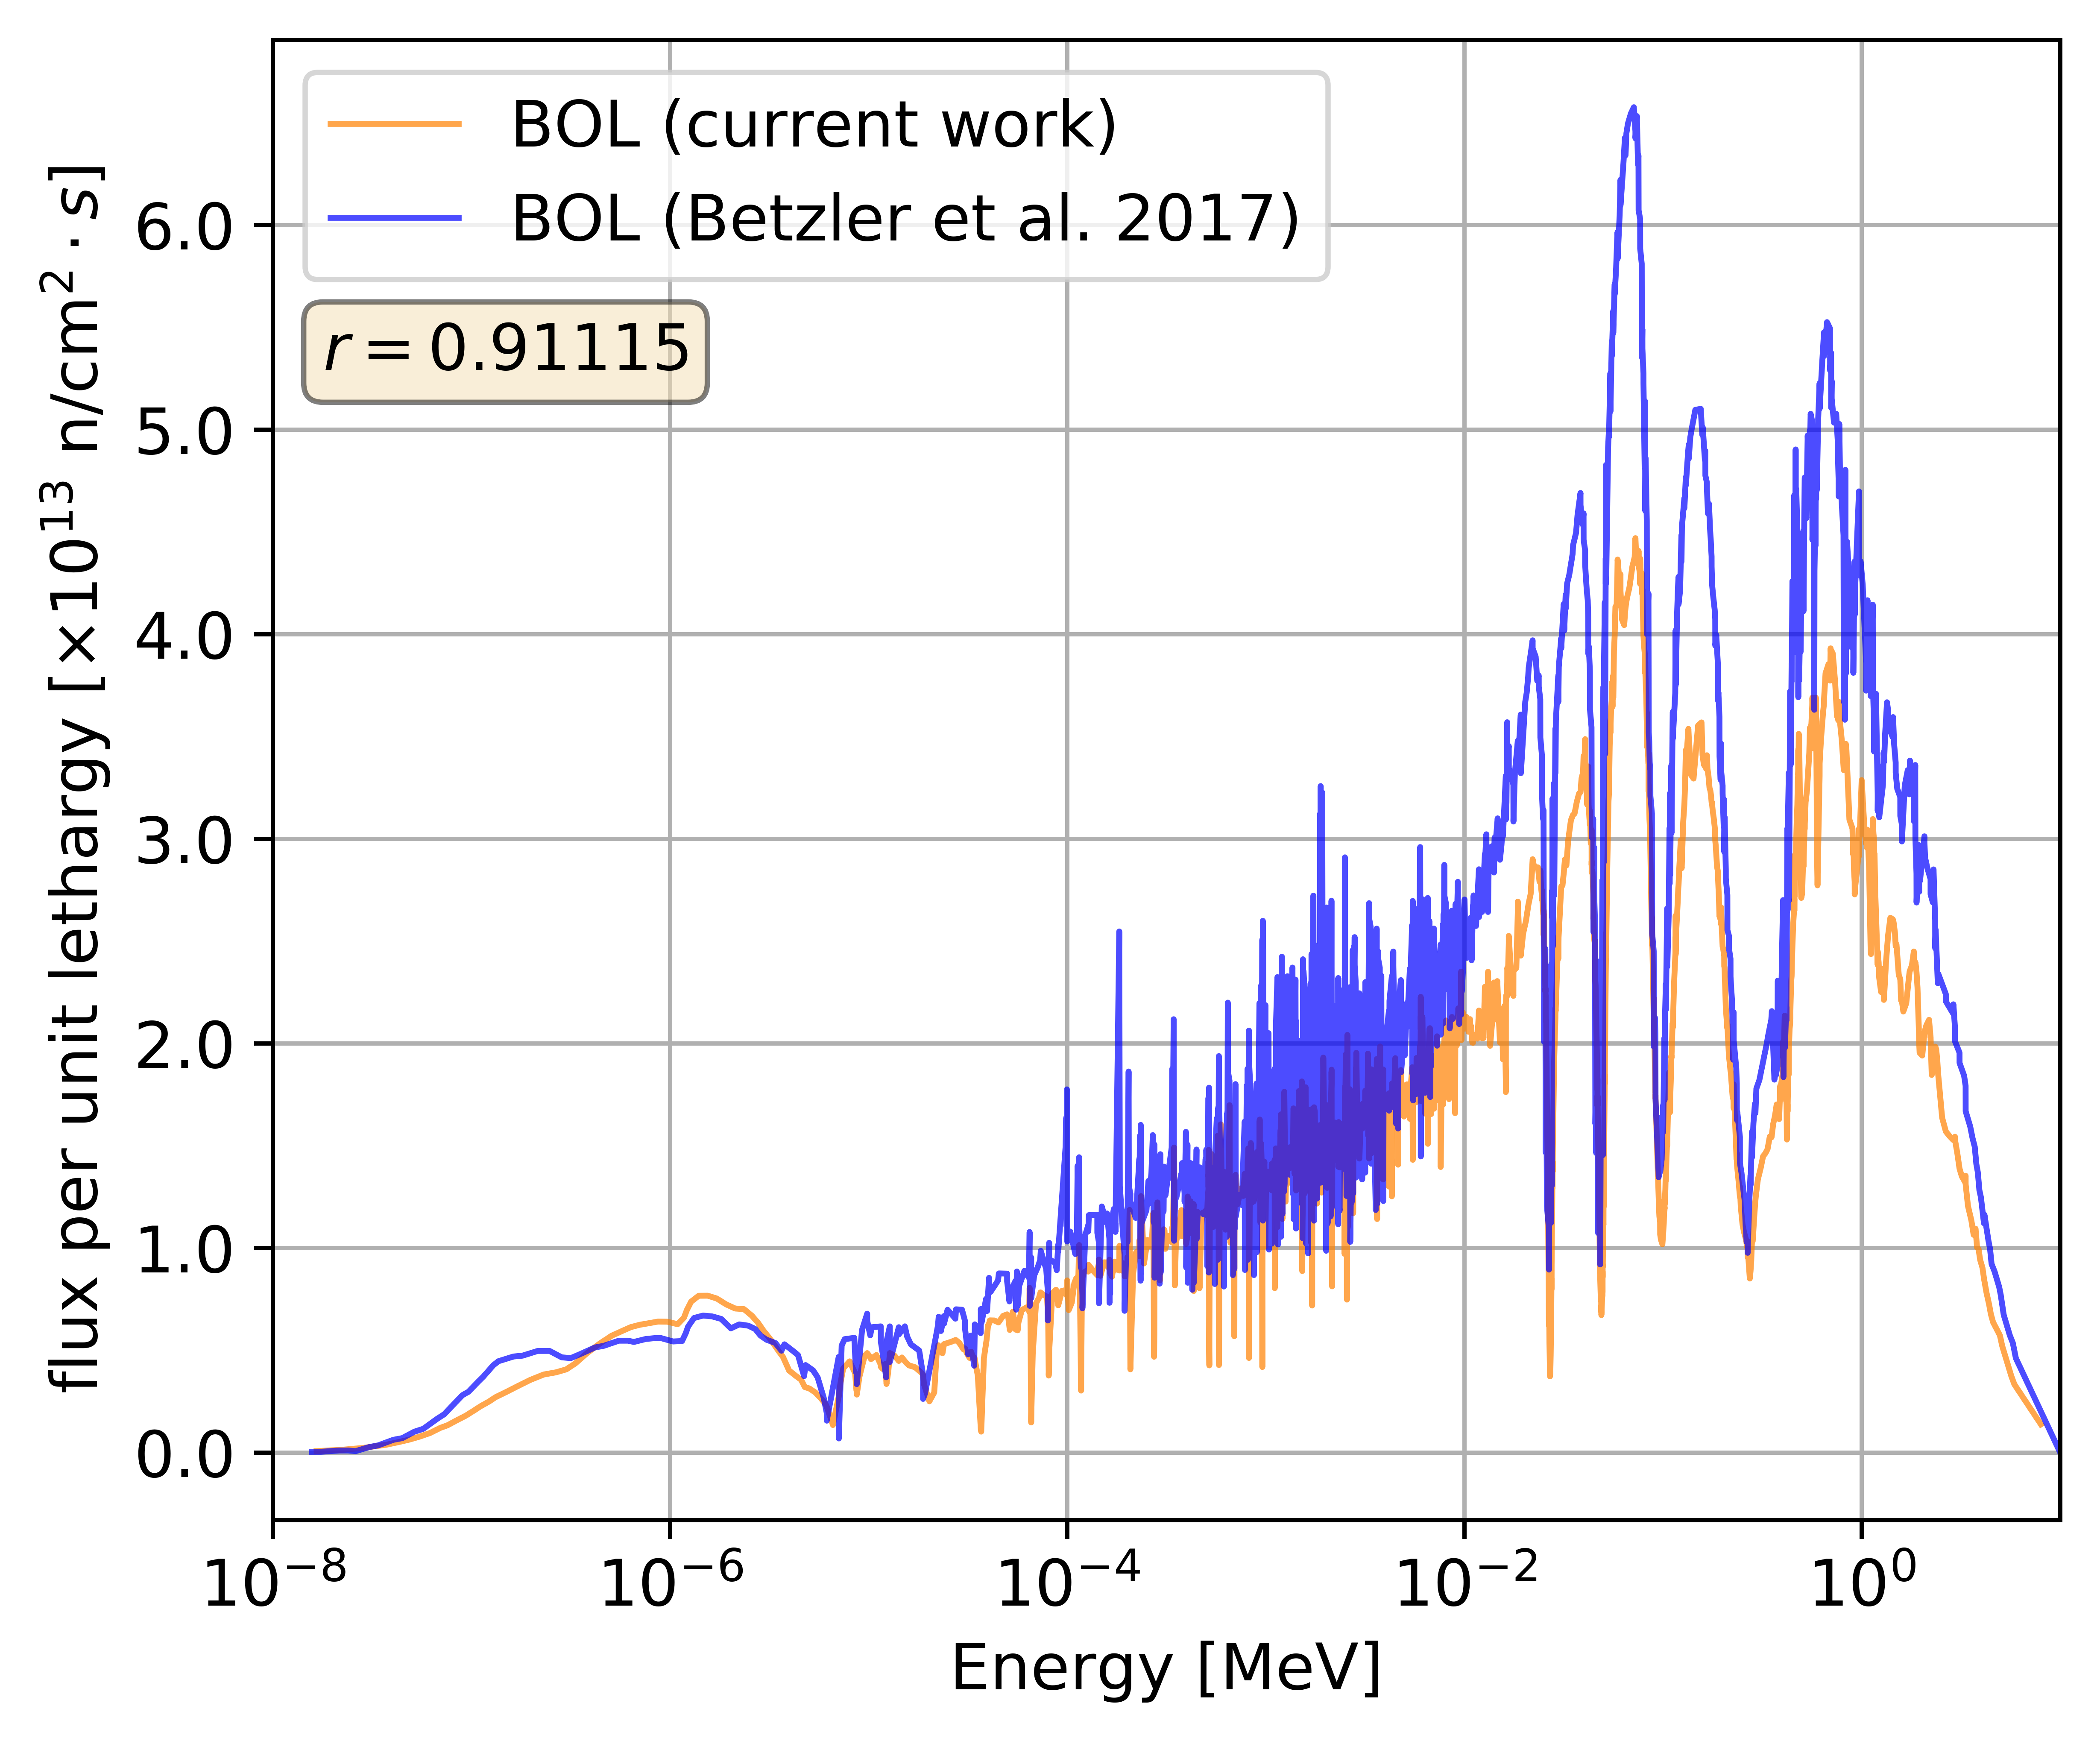
\includegraphics[width=0.77\textwidth]{ch4/ben_spec_bol.png}\\
	\vspace{-12mm}
	\hspace{0.5mm}
	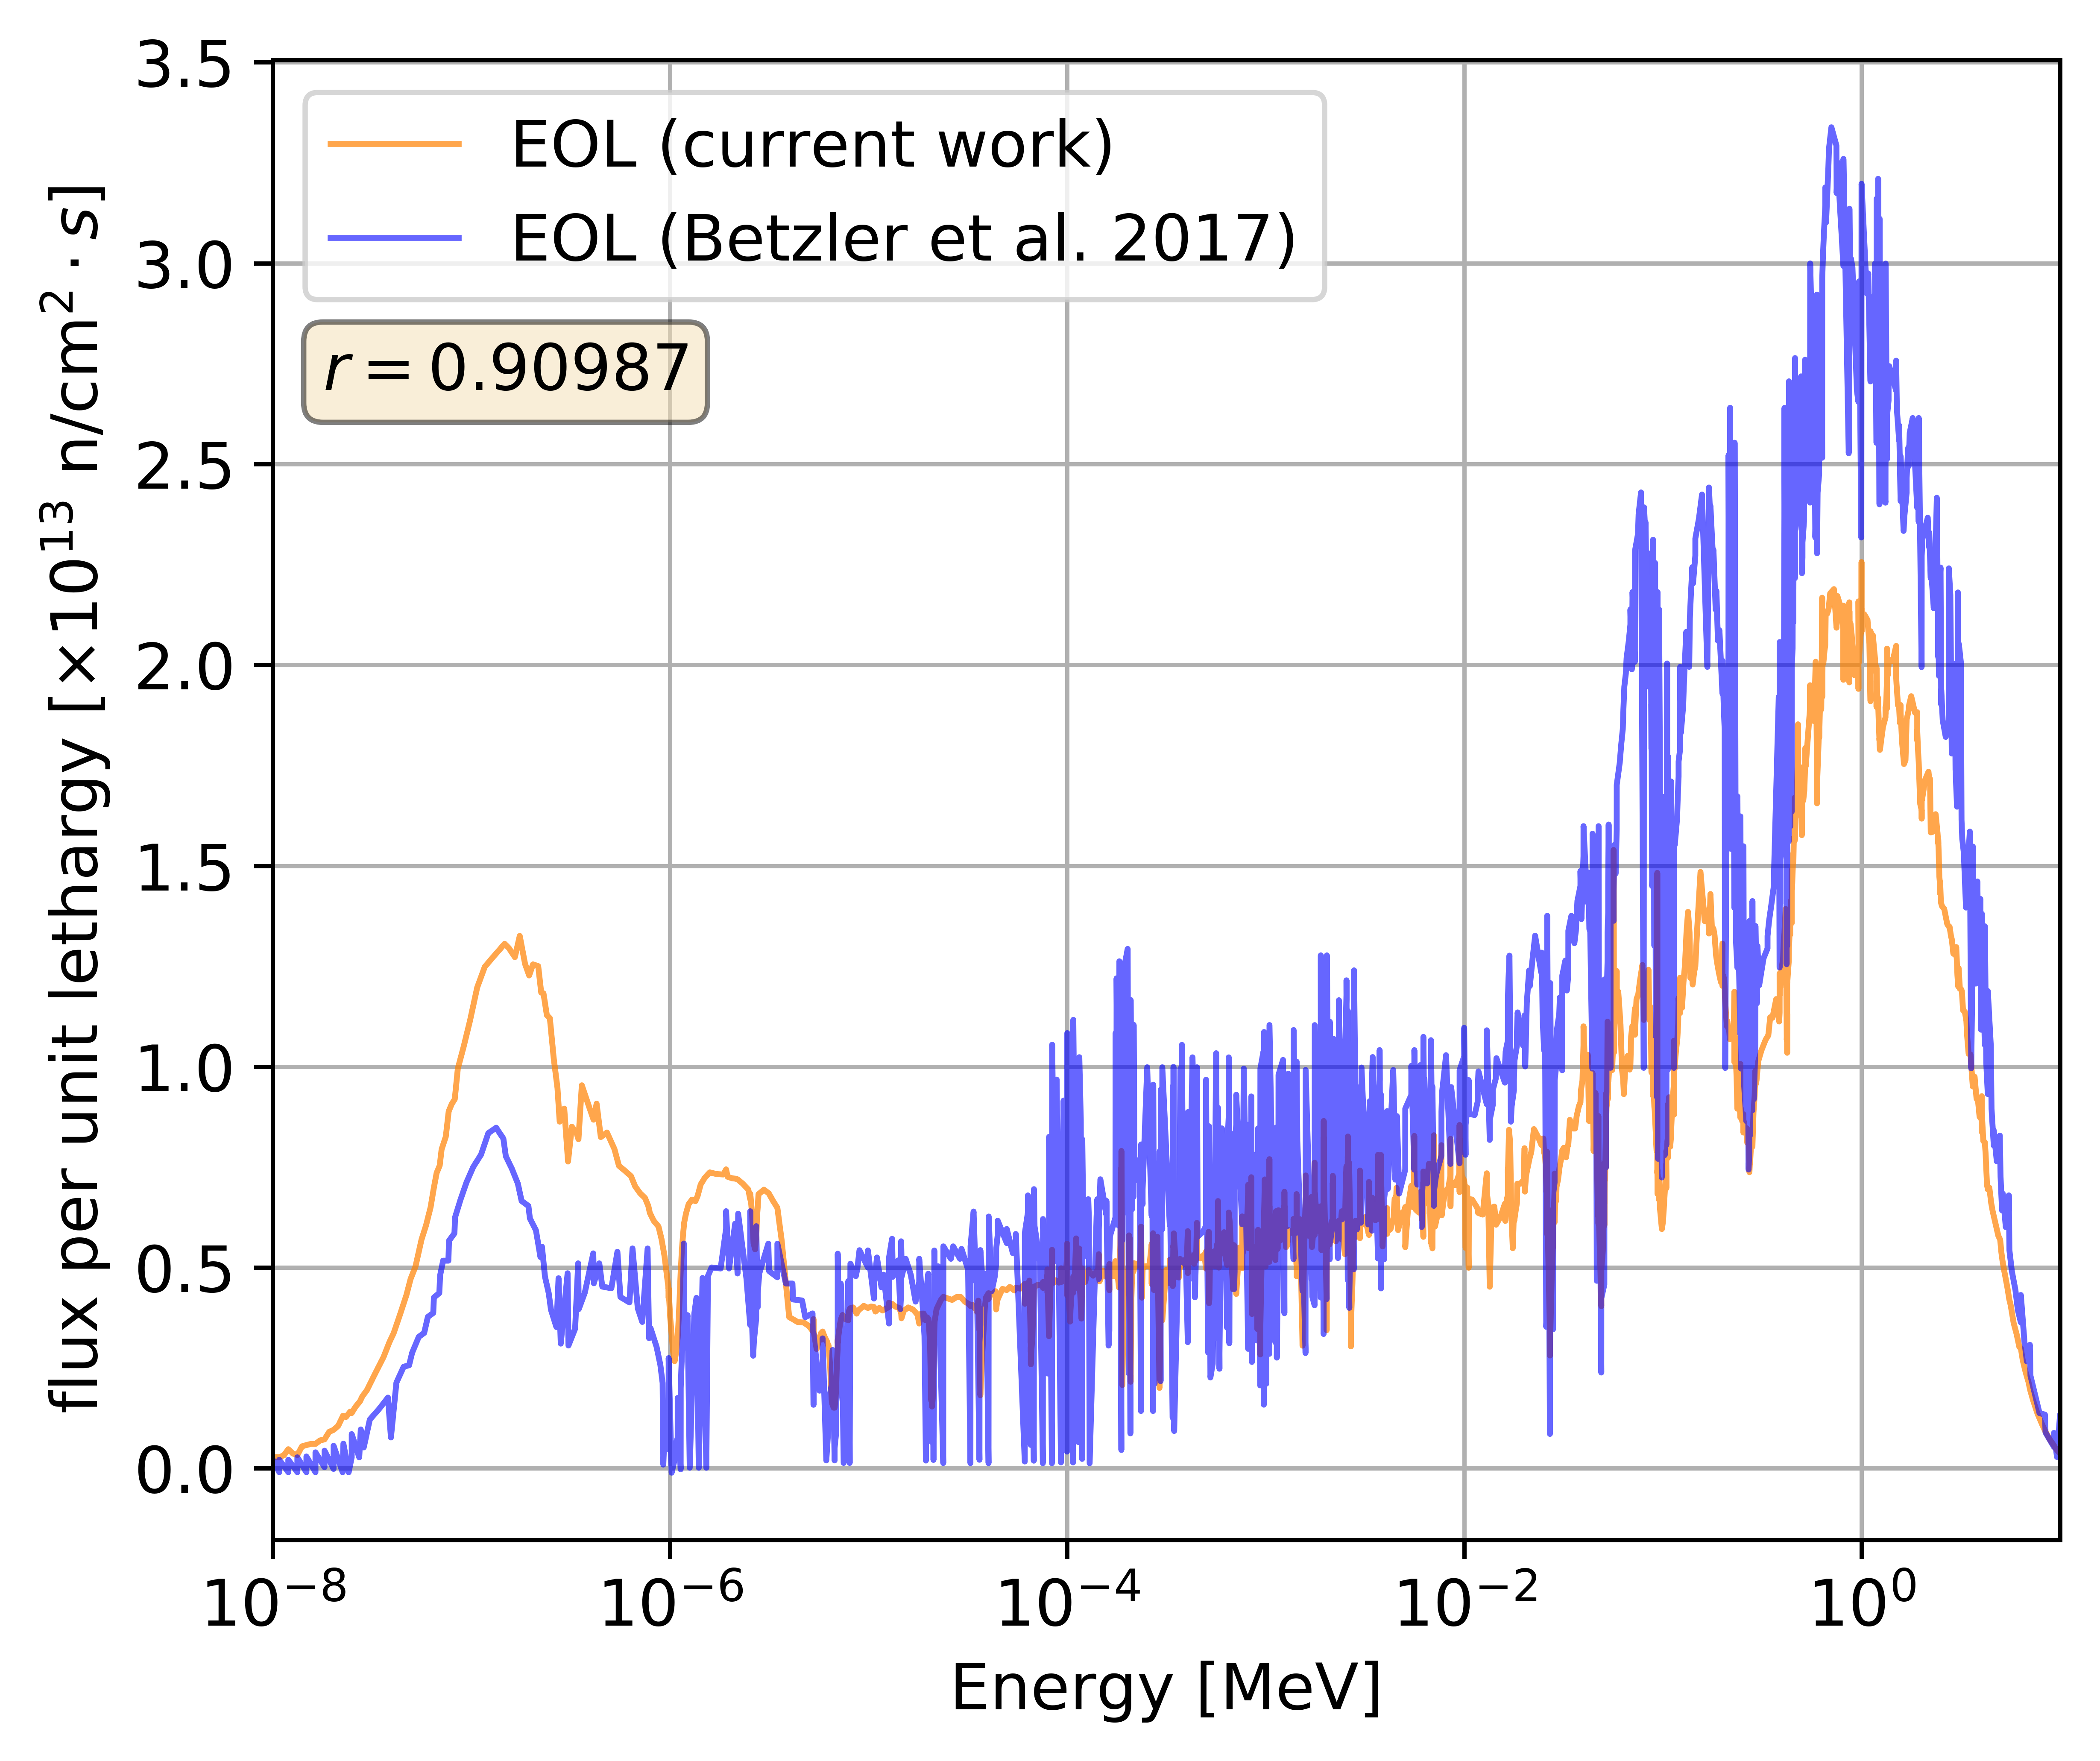
\includegraphics[width=0.77\textwidth]{ch4/ben_spec_eol.png}
	\vspace{-3mm}
	\caption{Neutron flux energy spectrum at the BOL (upper) and the EOL 
		(lower) obtained using SaltProc/Serpent (orange) compared with 
		ChemTriton/Shift (blue) \cite{betzler_assessment_2017-1}.}
	\label{fig:ben-spectrum-bol}
\end{figure}

The harder spectrum at the \gls{BOL} tends to significantly increase resonance 
absorption in $^{238}$U and decrease the absorptions in fissile and 
construction materials. Thus, the softer spectrum in the current work compared 
with Betzler \emph{et al.} led to fewer resonance captures\footnote{The energy 
range for $^{238}$U resonance neutron capture is between 10$^{-5}$ and 
10$^{-2}$ MeV.} of neutrons by $^{238}$U, hence, less $^{239}$Pu bred from 
$^{238}$U. Therefore, the SaltProc/Serpent calculation in the current work 
underpredicts the destruction (i.e., fission and capture) of $^{235}$U and 
overpredicts the destruction of $^{238}$U (see 
Table~\ref{tab:valid_ben_isos}). 
Finally, the softer neutron spectrum leads to more fissions in fissile 
plutonium isotopes ($^{239}$Pu and $^{241}$Pu) which also decreases 
non-fissile plutonium (Table~\ref{tab:valid_ben_isos}) and total actinide 
waste production (Table~\ref{tab:valid_ben_performance}).


\subsubsection{Time step refinement}\label{sec:time-refinement}
The results shown in this chapter are obtained from SaltProc calculations with 
a uniform depletion time step of 3 days. The duration of the time step was 
chosen after performing a parametric sweep to determine the longest depletion 
time step that provides suitable calculation accuracy. A longer time 
step potentially reduces the SaltProc calculation costs, providing results 
faster for lifetime-long (25-year) simulations. 

Figure~\ref{fig:timeref-keff} shows $k_{eff}$ evolution obtained with 3-, 6-, 
12-, and 24-day depletion time intervals for a 25-year simulation. The 
interval between moderator configuration updates was assumed similar for all 
four cases for consistency. The multiplication factor at the \gls{BOC} for 
each moderator configuration reduced with increasing time step duration. At 
the \gls{EOC} for each geometry, $k_{eff}=1.0$ for a 3-day time step but 
drops below 1.0 to 0.9980, 0.9972, and 0.9948 for 6-, 12-, and 24-day step, 
respectively. 
The 
decrease is because more poisonous \glspl{FP} (e.g., $^{135}$Xe) are produced 
in the core during longer depletion intervals. With longer time steps, a large 
concentration of poisons is obtained at the end of the depletion step when 
those poisons are being removed, resulting in substantial criticality 
growth. 

Figures~\ref{fig:timeref-u} and \ref{fig:timeref-pu239} show that the longer 
time steps appropriately capture uranium depletion ($<1$\% difference even for 
a 24-day time step), but the observed difference in fissile $^{239}$Pu mass is 
significant when the depletion interval is 6 days or longer ($>0.5$\% 
difference for 6-day step). Using a 6-day depletion interval leads to 
overprediction of $^{239}$Pu production by 5 kg at the \gls{EOL} 
(Figure~\ref{fig:timeref-pu239}). The use of a 6-day time step caused an 
overprediction of total plutonium production by 9.6 kg. Notably, 
significant quantity for plutonium currently in use by the IAEA is 8 kg 
($<80$\% $^{238}$Pu) \cite{close_iaea_1995}. Thus, a 6-day depletion interval 
or longer leads to significant error in the predicted plutonium inventory at 
the \gls{EOL} (larger than 1 significant quantity). 
\begin{figure}[hbp!] % replace 't' with 'b' to 
	\centering
	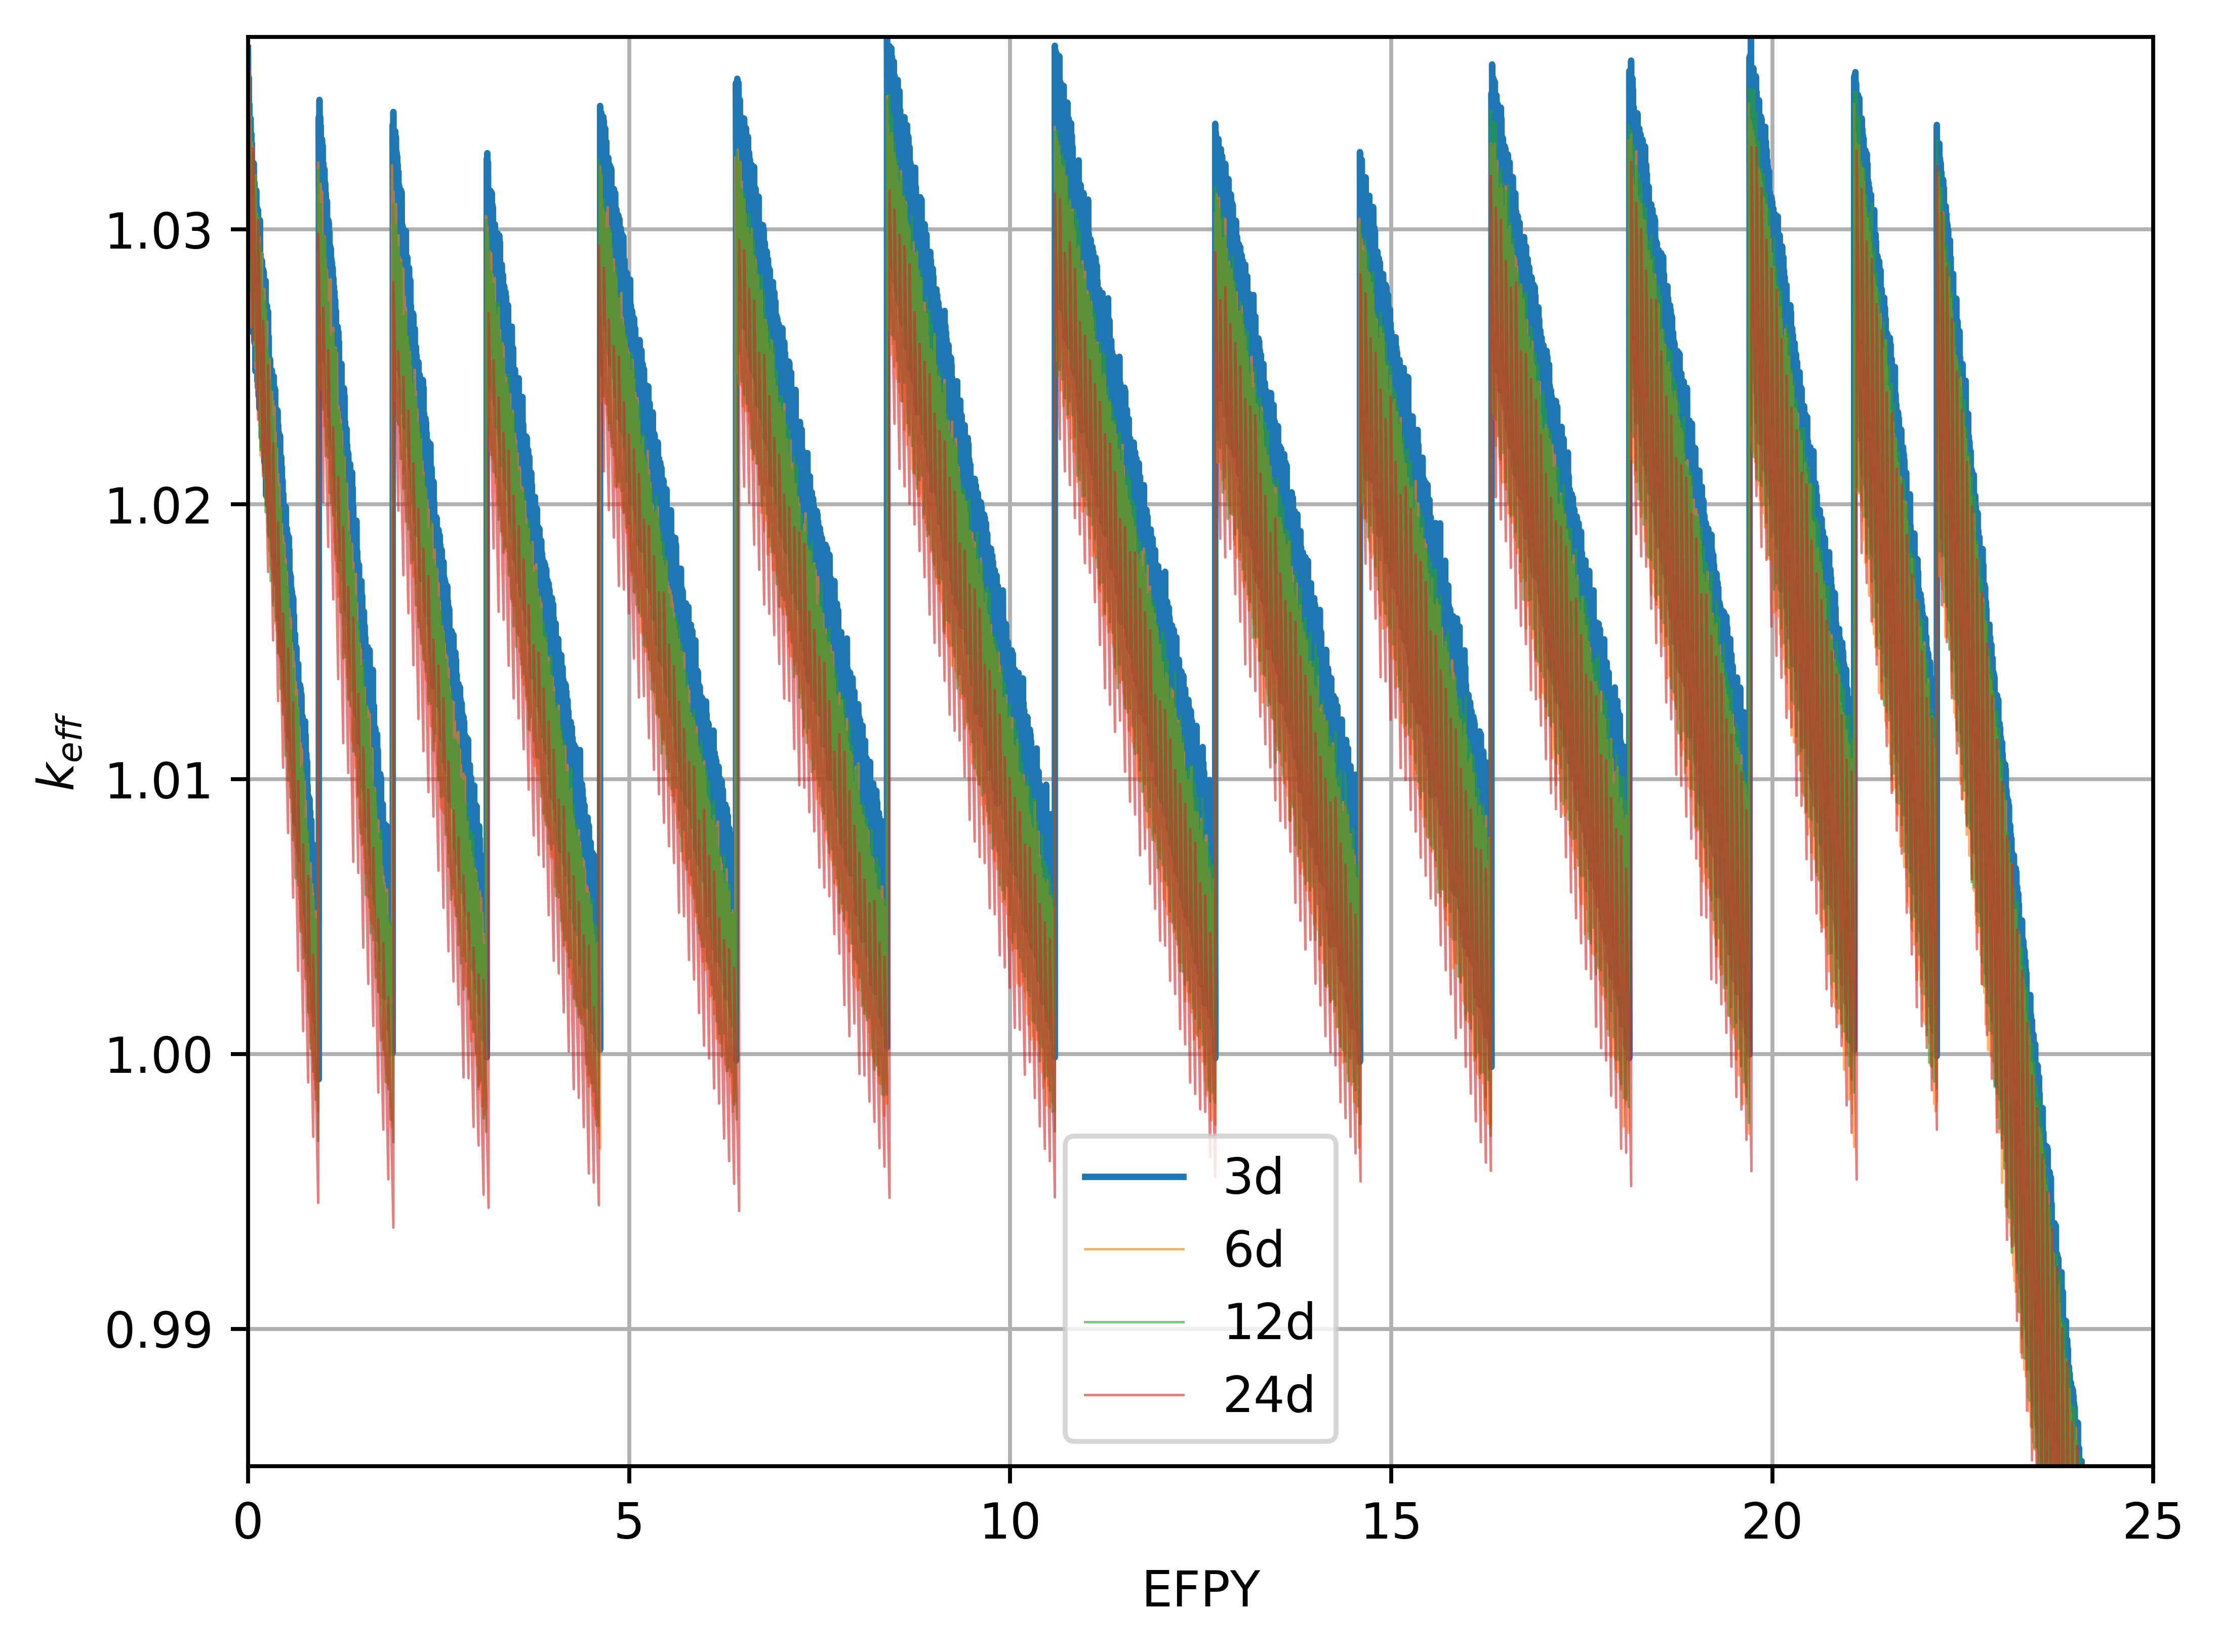
\includegraphics[width=\textwidth]{ch4/keff_time_refinement.png}
	\caption{SaltProc-calculated effective multiplication factor ($k_{eff}$) 
	during operation for different depletion time step sizes.}
	\label{fig:timeref-keff}
\end{figure}

\begin{figure}[hbp!] % replace 't' with 'b' to 
	\centering
	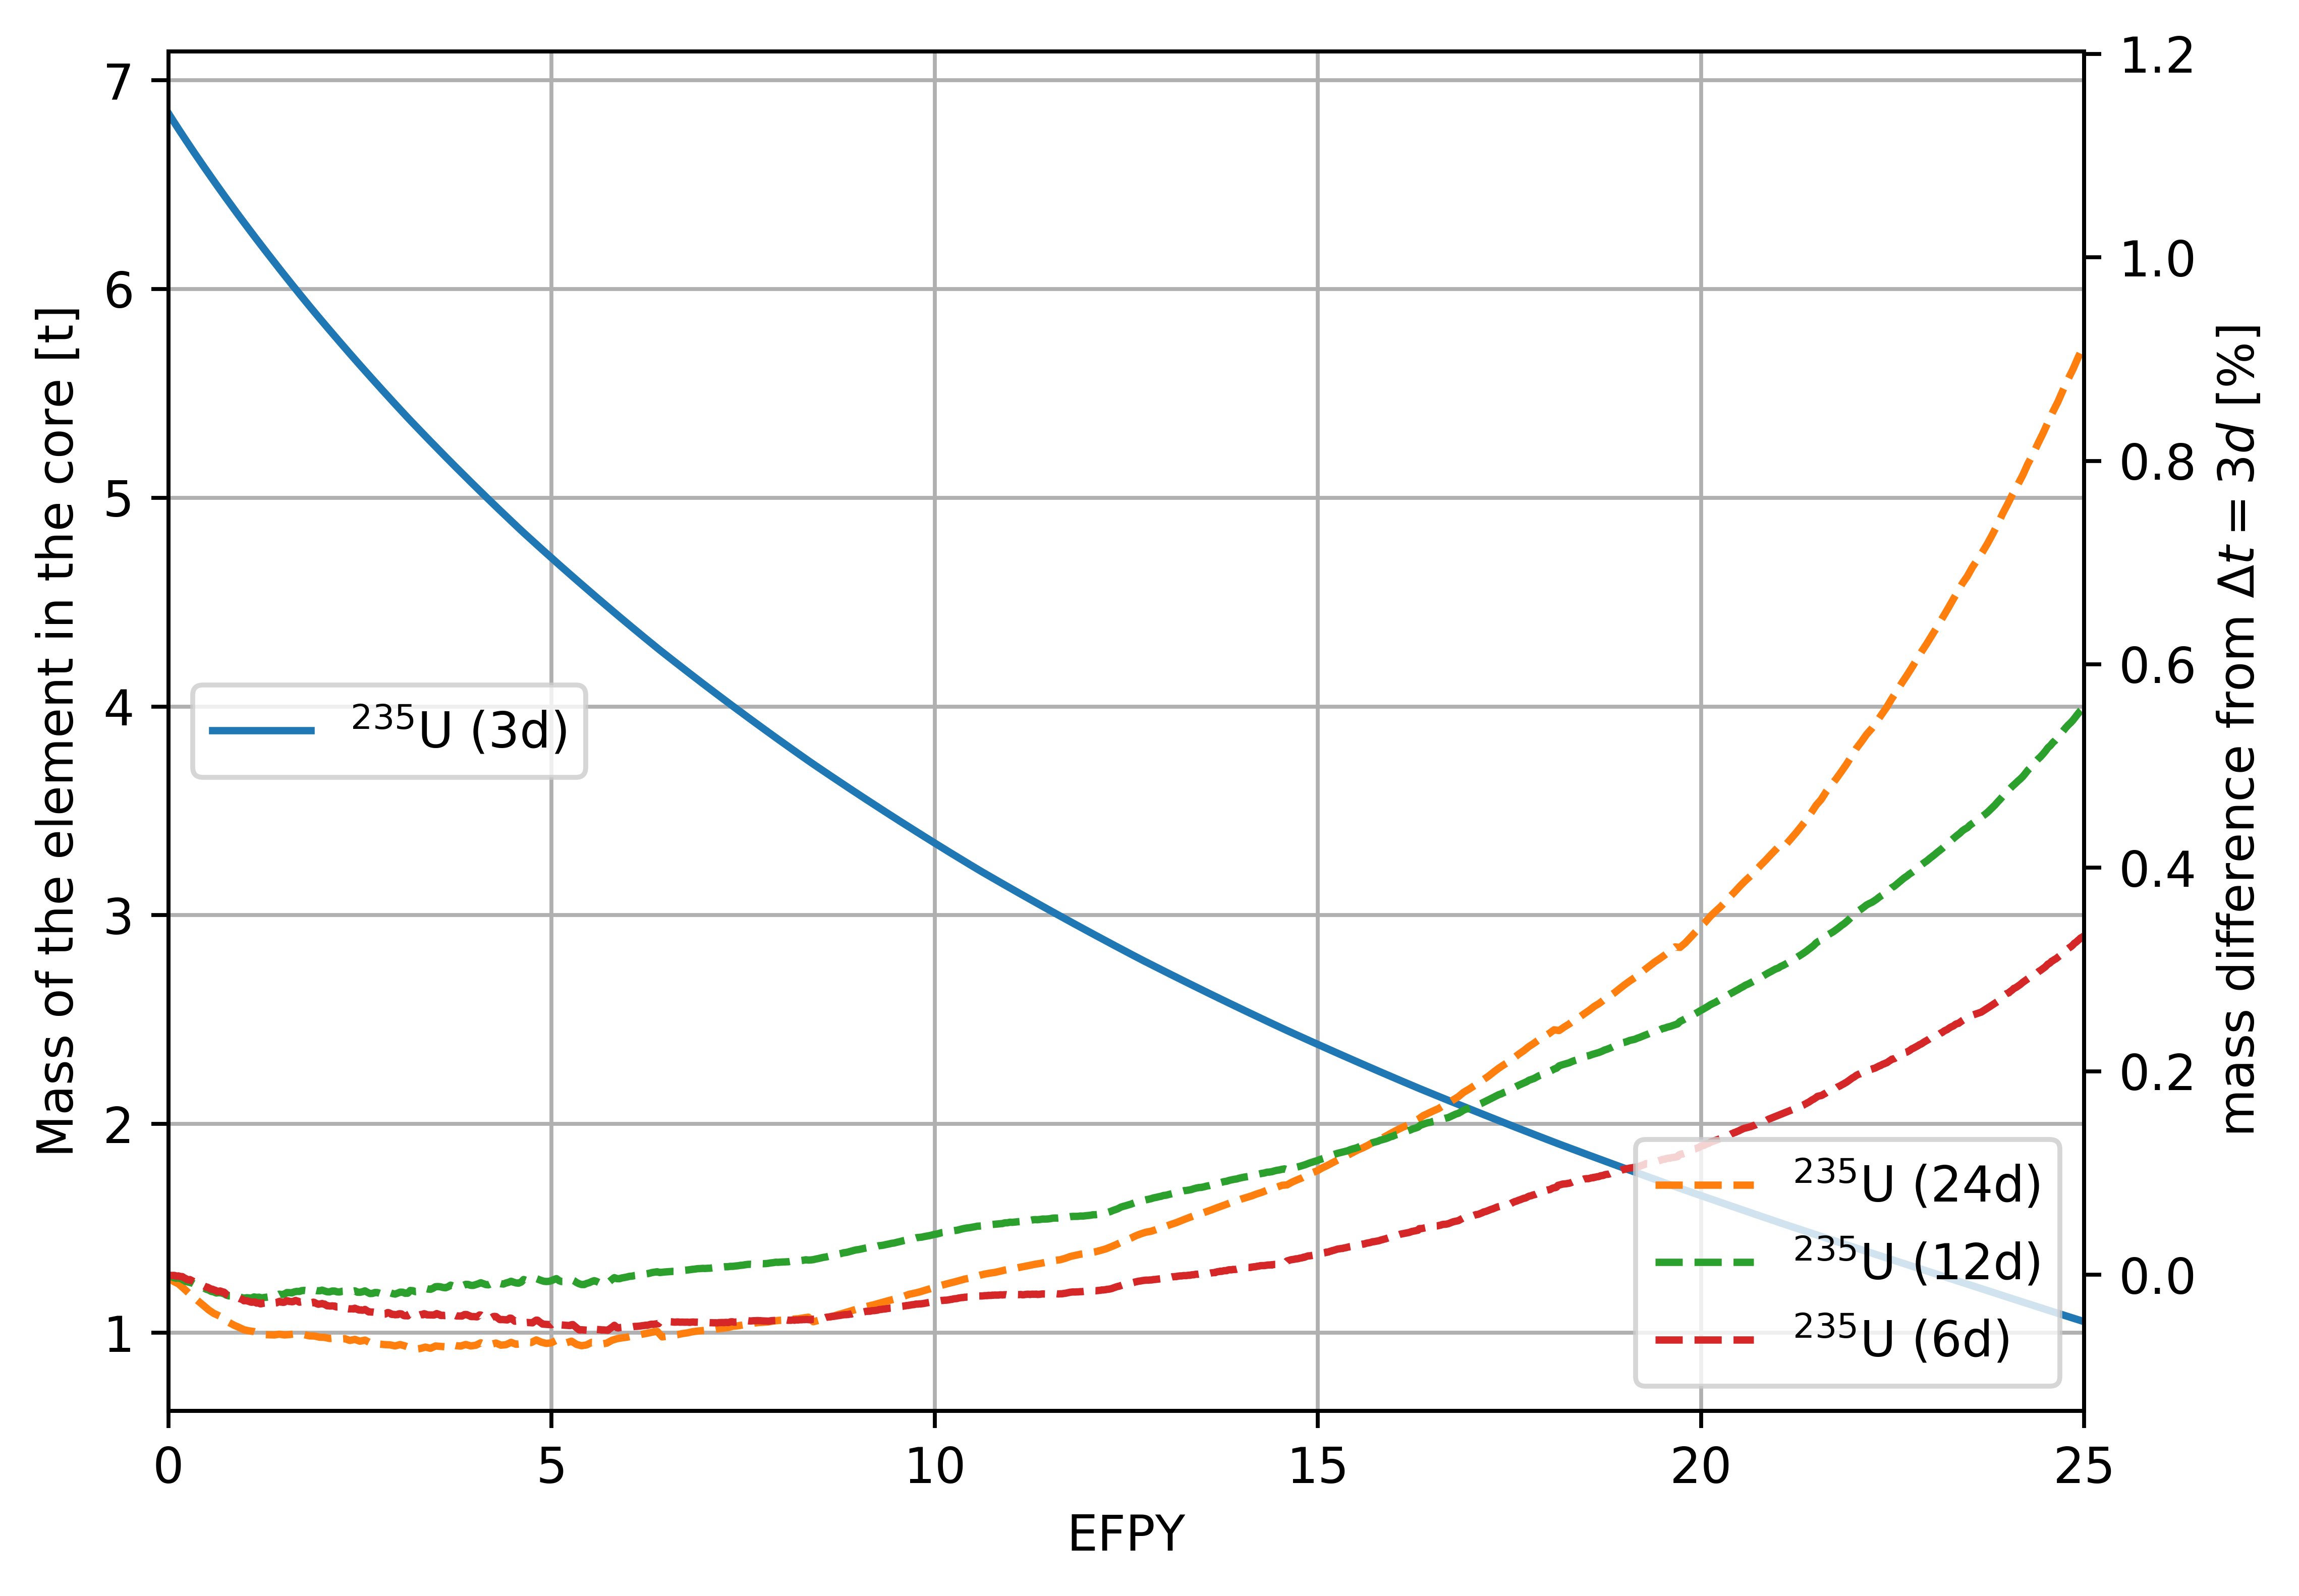
\includegraphics[width=0.91\textwidth]{ch4/u235_time_refinement.png}\\
		\vspace{-11mm}
	\hspace{0.5mm}
	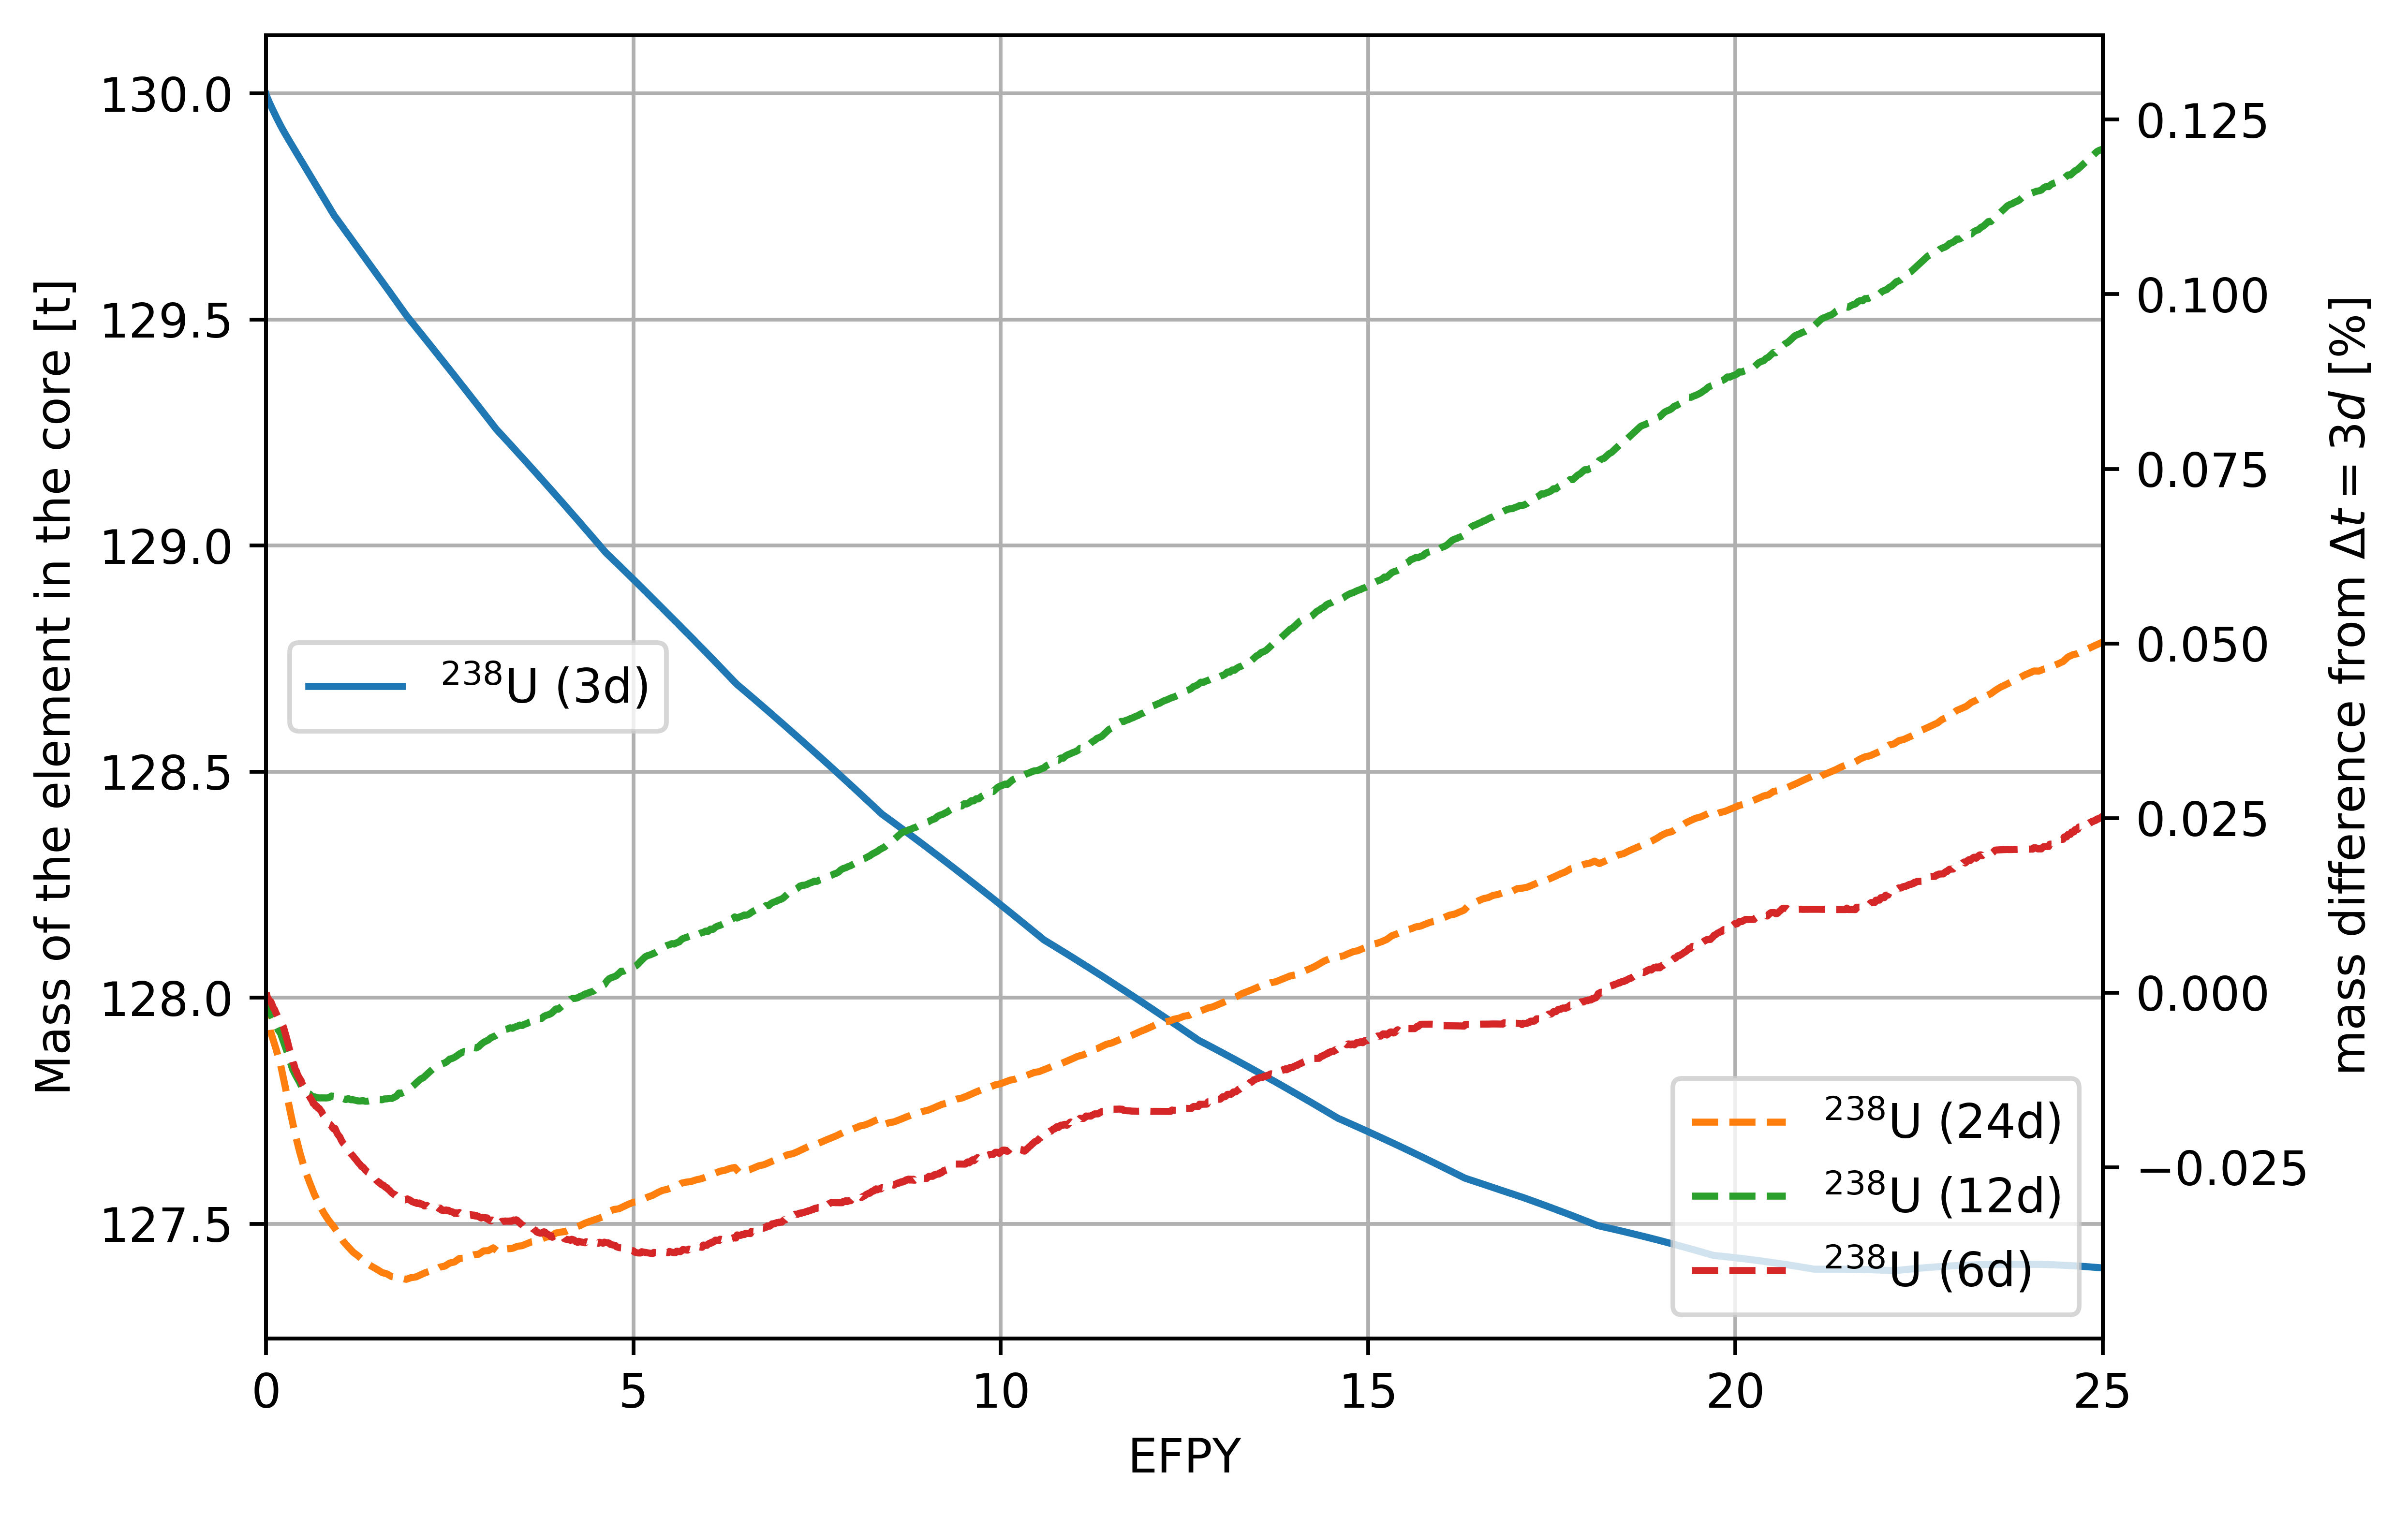
\includegraphics[width=\textwidth]{ch4/u238_time_refinement.png}
		\vspace{-6mm}
	\caption{SaltProc-calculated $^{235}$U (upper) and $^{238}$U (lower) 
	content during operation for different depletion time step sizes.}
	\label{fig:timeref-u}
\end{figure}

\begin{figure}[htp!] % replace 't' with 'b' to 
	\centering
	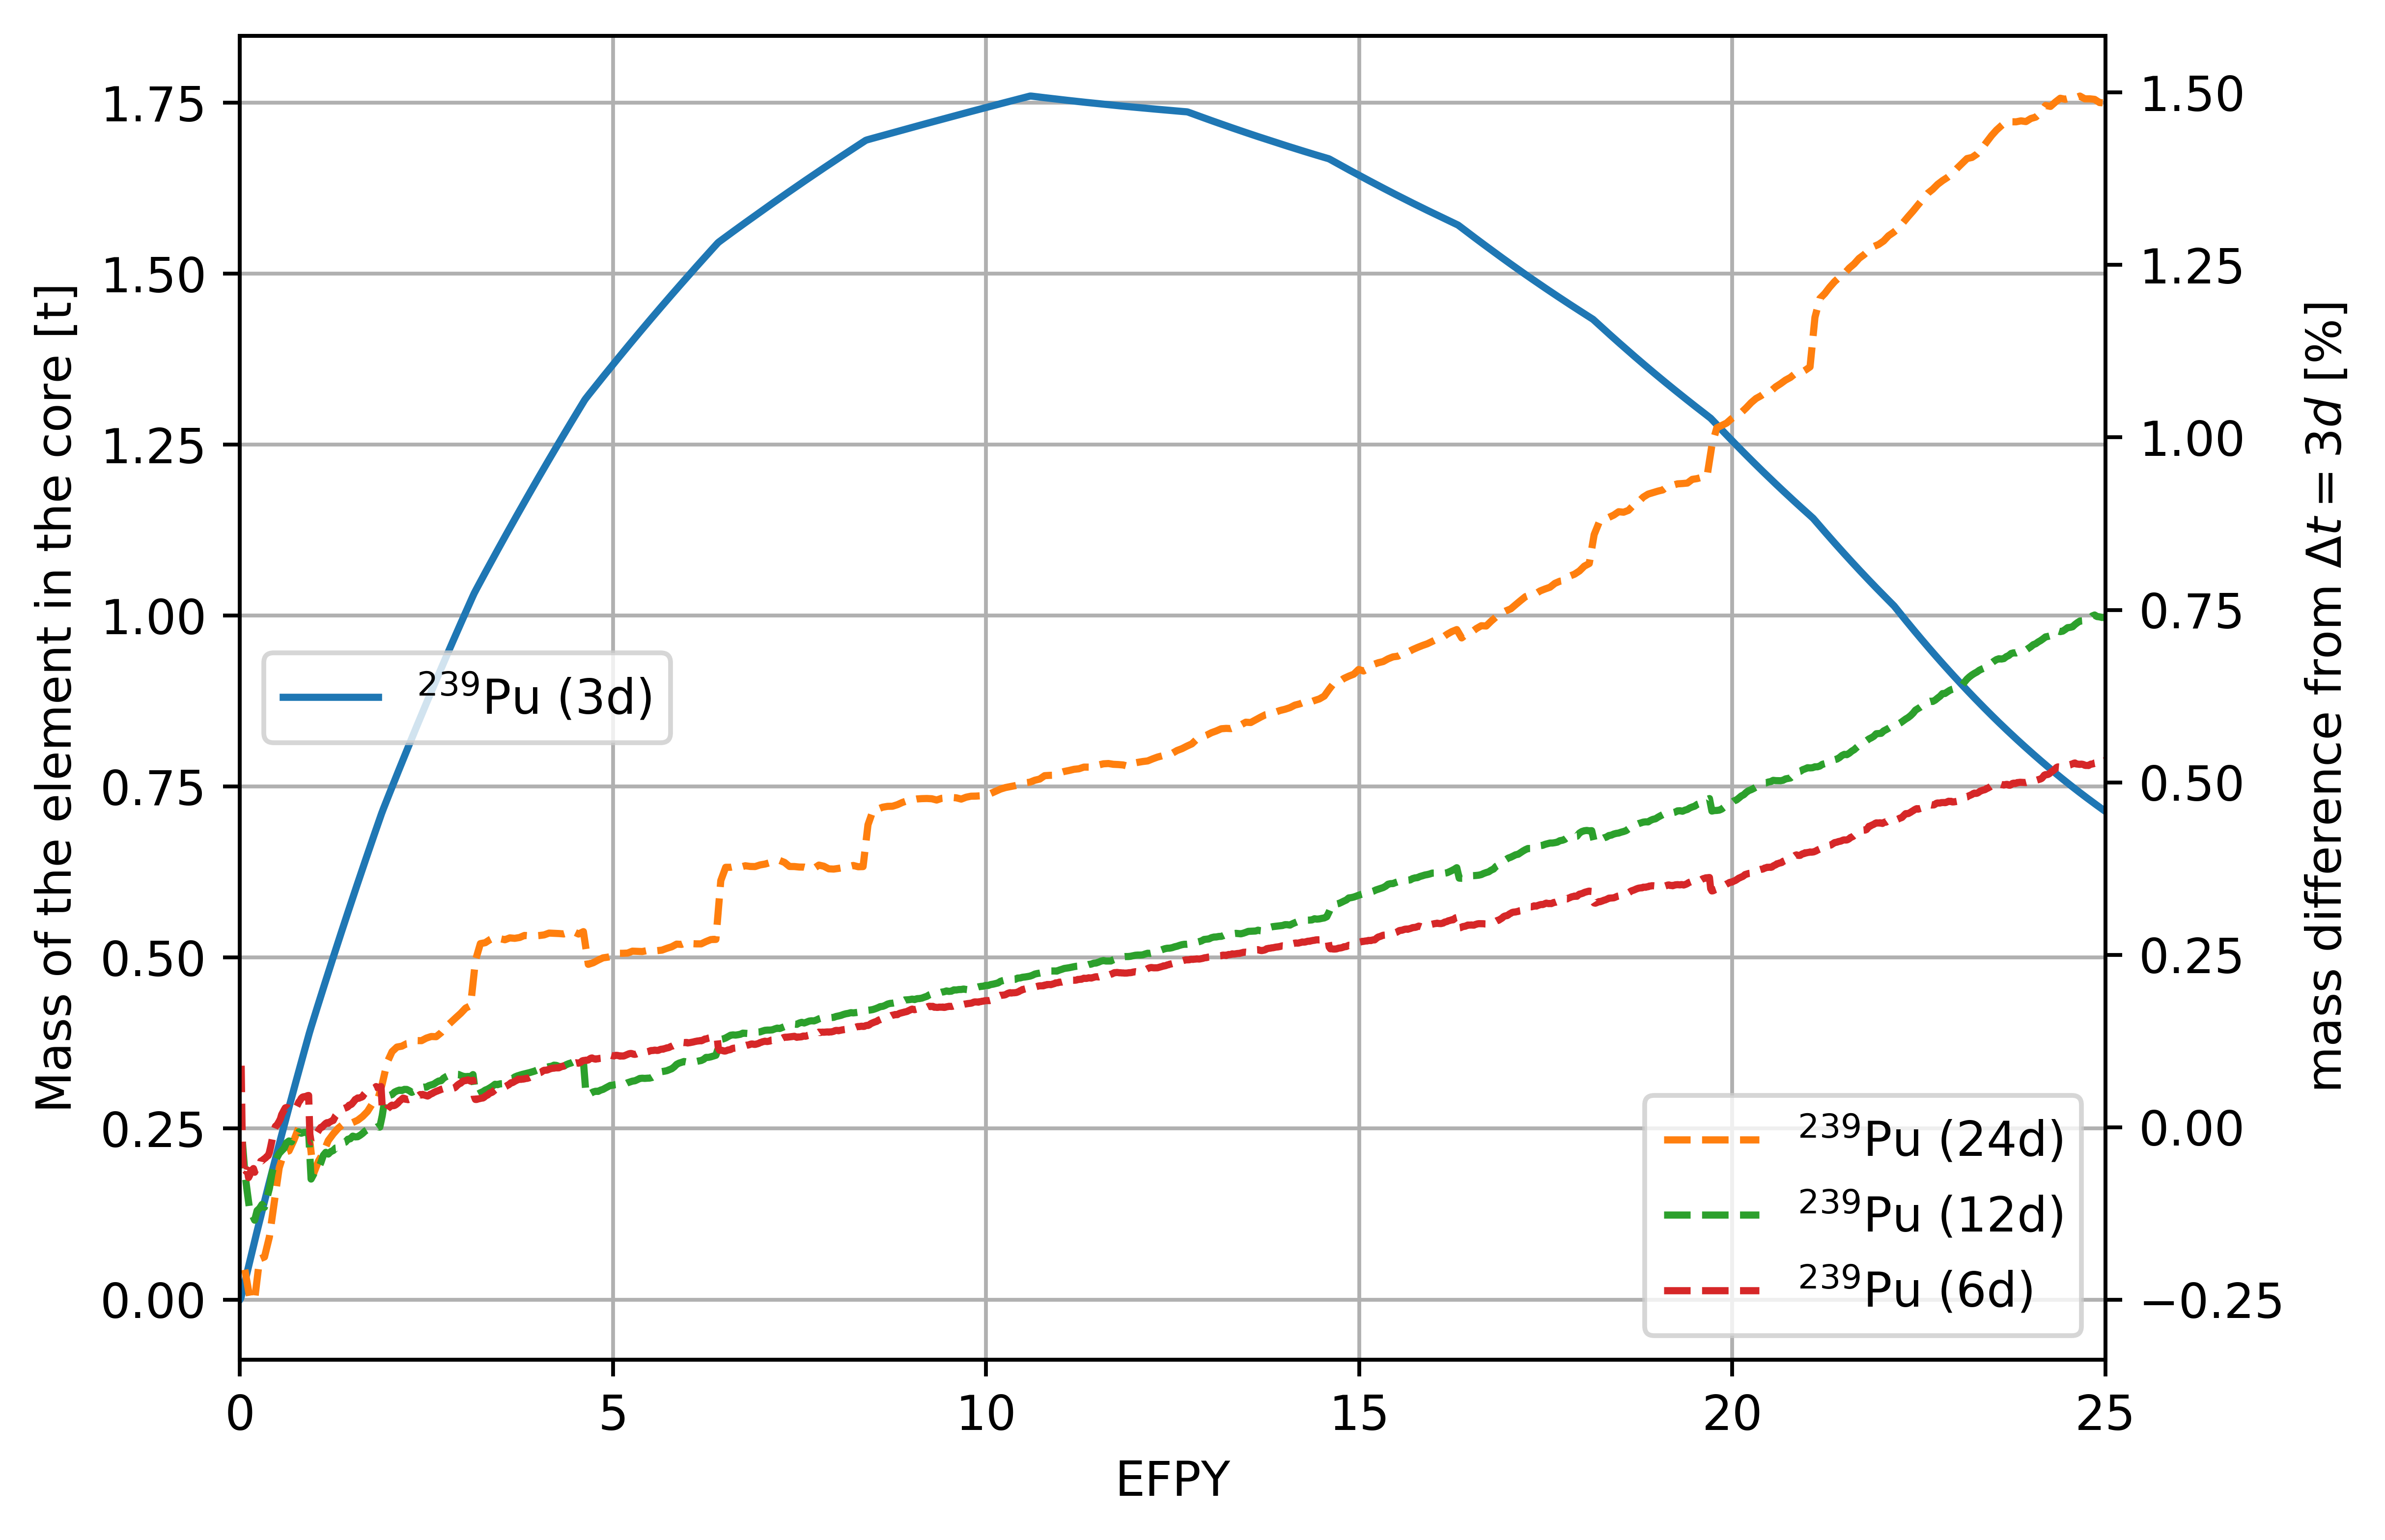
\includegraphics[width=\textwidth]{ch4/pu239_time_refinement.png}
	\caption{SaltProc-calculated $^{239}$Pu content during operation for 
		different depletion time step sizes.}
	\label{fig:timeref-pu239}
\end{figure}
Increasing the depletion time interval significantly reduces computational 
cost but also deteriorates the accuracy of depletion calculations (i.e., 
24-day step gave $\times4$ speedup but causes about 1.5\% error in $^{239}$Pu 
mass prediction). Calculations using a depletion time step of 6 days or more 
demonstrated a significant difference in calculated $k_{eff}$ (i.e., 
$\approx300$ $pcm$ for 6-day) and depleted 
mass (e.g., $\approx0.34$\% error in $^{235}$U predicted mass for 6-day) from 
those using a 3-day depletion step. \emph{In the current work, a 3-day 
depletion step was selected to adequately predict the mass of major heavy 
isotopes in the fuel salt during 25 years of the \gls{TAP} reactor operation.}


\subsection{Realistic extraction efficiency case}\label{sec:long-term-real}
This section demonstrates SaltProc v1.0 for lifetime-long depletion simulation 
similar to Section~\ref{sec:ben-valid}, but with realistic, physics-based 
correlations for noble gas removal efficiency. For the demonstration case 
herein, efficiency of xenon, krypton, and hydrogen extraction are determined 
using the model by Peebles \emph{et al.} (Equation~\ref{eq:gas_eff}) discussed 
earlier in Section~\ref{sec:gas-separ}. The gas-liquid interfacial area per 
unit volume ($a$) to inform 
Equation~\ref{eq:gas_eff} is a function of salt/gas flow rates and gas bubble 
diameter \cite{sada_gas-liquid_1987}:
\begin{align}\label{eq:interfacial-area}
& a = \frac{6}{d_b}\frac{Q_{He}}{Q_{He} + Q_{salt}}
\intertext{where}
Q_{salt}&= \mbox{volumetric salt flow rate $[m^3/s]$} \nonumber \\
Q_{He}&= \mbox{volumetric helium flow rate $[m^3/s]$} \nonumber \\
d_b &= \mbox{helium bubble diameter $[m]$.} \nonumber
\end{align}

Additionally, the following parameters inform 
Equation~\ref{eq:gas_eff} for the prototypic sparger: (1) salt volumetric flow 
rate throughout the sparger $Q_{salt}=2$ $m^3/s$; (2) sparging gas (helium) 
volumetric flow rate $Q_{He}=0.1$ $m^3/s$; (3) helium bubble diameter 
$d_b=0.508$ $mm$ as advised by ORNL \cite{robertson_conceptual_1971}; (4) 
sparger length $L=11$ $m$; (5) sparger diameter $D=0.4$ $m$ (sparger 
cross section $A_C=0.126$ $m^2$).

The liquid phase mass transfer coefficient ($K_L$) selection presents a 
challenge since published information to inform 
Equation~\ref{eq:gas_eff} is applicable for only laboratory-scale conditions 
\cite{chen_cfd_2019-1}. 
Peebles \emph{et al.} stated that Equation~\ref{eq:gas_eff} is valid for $K_L$
in a range from 1 to 100 $ft/hr$ (from $0.084\bar{7}$ to $8.47\bar{7}$ $mm/s$) 
\cite{peebles_removal_1968}. For the demonstration case herein, I performed 
25-year depletion calculations for $K_L$ of $0.084\bar{7}$, 2.1167, and 
$8.466\bar{7}$ $mm/s$ 
to investigate the effect of noble gas removal efficiency on lifetime-long 
fuel depletion calculations.

The extraction efficiency is gas specific because solubility in the salt 
(Henry's law constant) is different for various gases. 
Table~\ref{tab:gas_removal_efficiency} reports the dimensionless Henry's law 
constant and corresponding calculated efficiency of noble gas (Xe, Kr, H) 
migration to the helium bubbles ($\epsilon_m$) in the prototypic sparger for 
various mass transfer coefficients.  Total separation efficiency  
(Table~\ref{tab:gas_removal_efficiency}, last three columns) refers to the 
efficiency of extraction target gaseous elements after performing helium 
sparging in the sparger followed by separation of noble-gas-reach bubbles from 
the salt in the axial-flow centrifugal bubble separator 
\cite{gabbard_development_1974}. 


%%%%%%%%%%%%%%%%%%%%%%%%%%%%%%%%%%%%%%%%
\begin{table}[htp!]
	\fontsize{9}{11}\selectfont
	\centering
	\caption{The noble gas extraction efficiency at working temperature 
		T=627$^{\circ}$C calculated using Equation~\ref{eq:gas_eff} 
		\cite{peebles_removal_1968} assuming salt volumetric flow 
		rate $Q_{salt}=2$ $m^3/s$, helium volumetric flow rate $Q_{He}=0.1$ 
		$m^3/s$, helium bubbles diameter $d_b=0.508$ $mm$, and sparger volume
		$V=1.4$ $m^3$. The liquid phase mass transfer coefficient is varied in 
		validity range $[0.0847,8.4667]$ $mm/s$.}
	\begin{tabularx}{\textwidth}{L X R R R R R R}
		\hline 
		\textbf{Element}&\textbf{Henry's}& 
		\multicolumn{6}{c}{\textbf{Efficiency of}} \\
		& \textbf{law}& \multicolumn{3}{c}{\textbf{migration to He bubbles 
		($\epsilon_m$)}}& \multicolumn{3}{c}{\textbf{total separation 
		($\epsilon$)$^{\star}$}} \\
		&\textbf{constant} & \multicolumn{3}{c}{\textbf{for $K_L$ [mm/s]}} 
		&\multicolumn{3}{c}{\textbf{for $K_L$ [mm/s]}}\\
		&\textbf{($K_H$)$[-]$} & 8.4667&2.1167&0.0847&8.4667&2.1167&0.0847\\
		\hline
		Xe &5.7E-5 \cite{blander_solubility_1959}&0.9630&0.5639&0.0327&	
		0.9149&0.5357&0.0310\\
		Kr &2.8E-4 \cite{blander_solubility_1959}&0.9595&0.5630&0.0327& 
		0.9115&0.5349&0.0310\\
		H  &3.9E-3\cite{tomkins_gases_2016}&0.9066&0.5499&0.0326&
		0.8613&0.5224&0.0309\\	
		\hline
	\end{tabularx}
	\begin{tablenotes}
		\footnotesize
		\item$^{\star}$With axial-flow centrifugal bubble separator by 
		Gabbard \emph{et al.}, which allows the bubble separation efficiency 
		$\epsilon_{es}$=0.95 \cite{gabbard_development_1974}. Thus, total 
		gas removal efficiency ($\epsilon$) can be calculated as follows: 
		$\epsilon=\epsilon_m\times \epsilon_{es}$.
	\end{tablenotes}
	\label{tab:gas_removal_efficiency}
	\vspace{-0.9em}
\end{table}
%%%%%%%%%%%%%%%%%%%%%%%%%%%%%%%%%%%%%%%%%%%%%%%%%%%%%%%%%%%%%%%%%%%%%%%%%%%%%%%


\subsubsection{Effective multiplication factor dynamics}
Figures~\ref{fig:keff-eps-var} and \ref{fig:keff-eps-var-zoom} demonstrate the 
effective multiplication factor dynamics ($k_{eff}$) 
during 25 years of operation with 15 various moderator rod configurations 
(cycles) described in Appendix~A. SaltProc v1.0 
coupled to Serpent calculated 
$k_{eff}$ after removing fission products and feeding 5\% \gls{LEU} at the end 
of each depletion step (3 days as was determined in 
Section~\ref{sec:time-refinement}). Notably, the core went subcritical during 
the first cycle (startup moderator rod configuration) after 330 and 318 days 
for $K_L=8.4667$ and 0.0847 $mm/s$, respectively. 
\begin{figure}[htp!] % replace 't' with 'b' to 
	\centering
	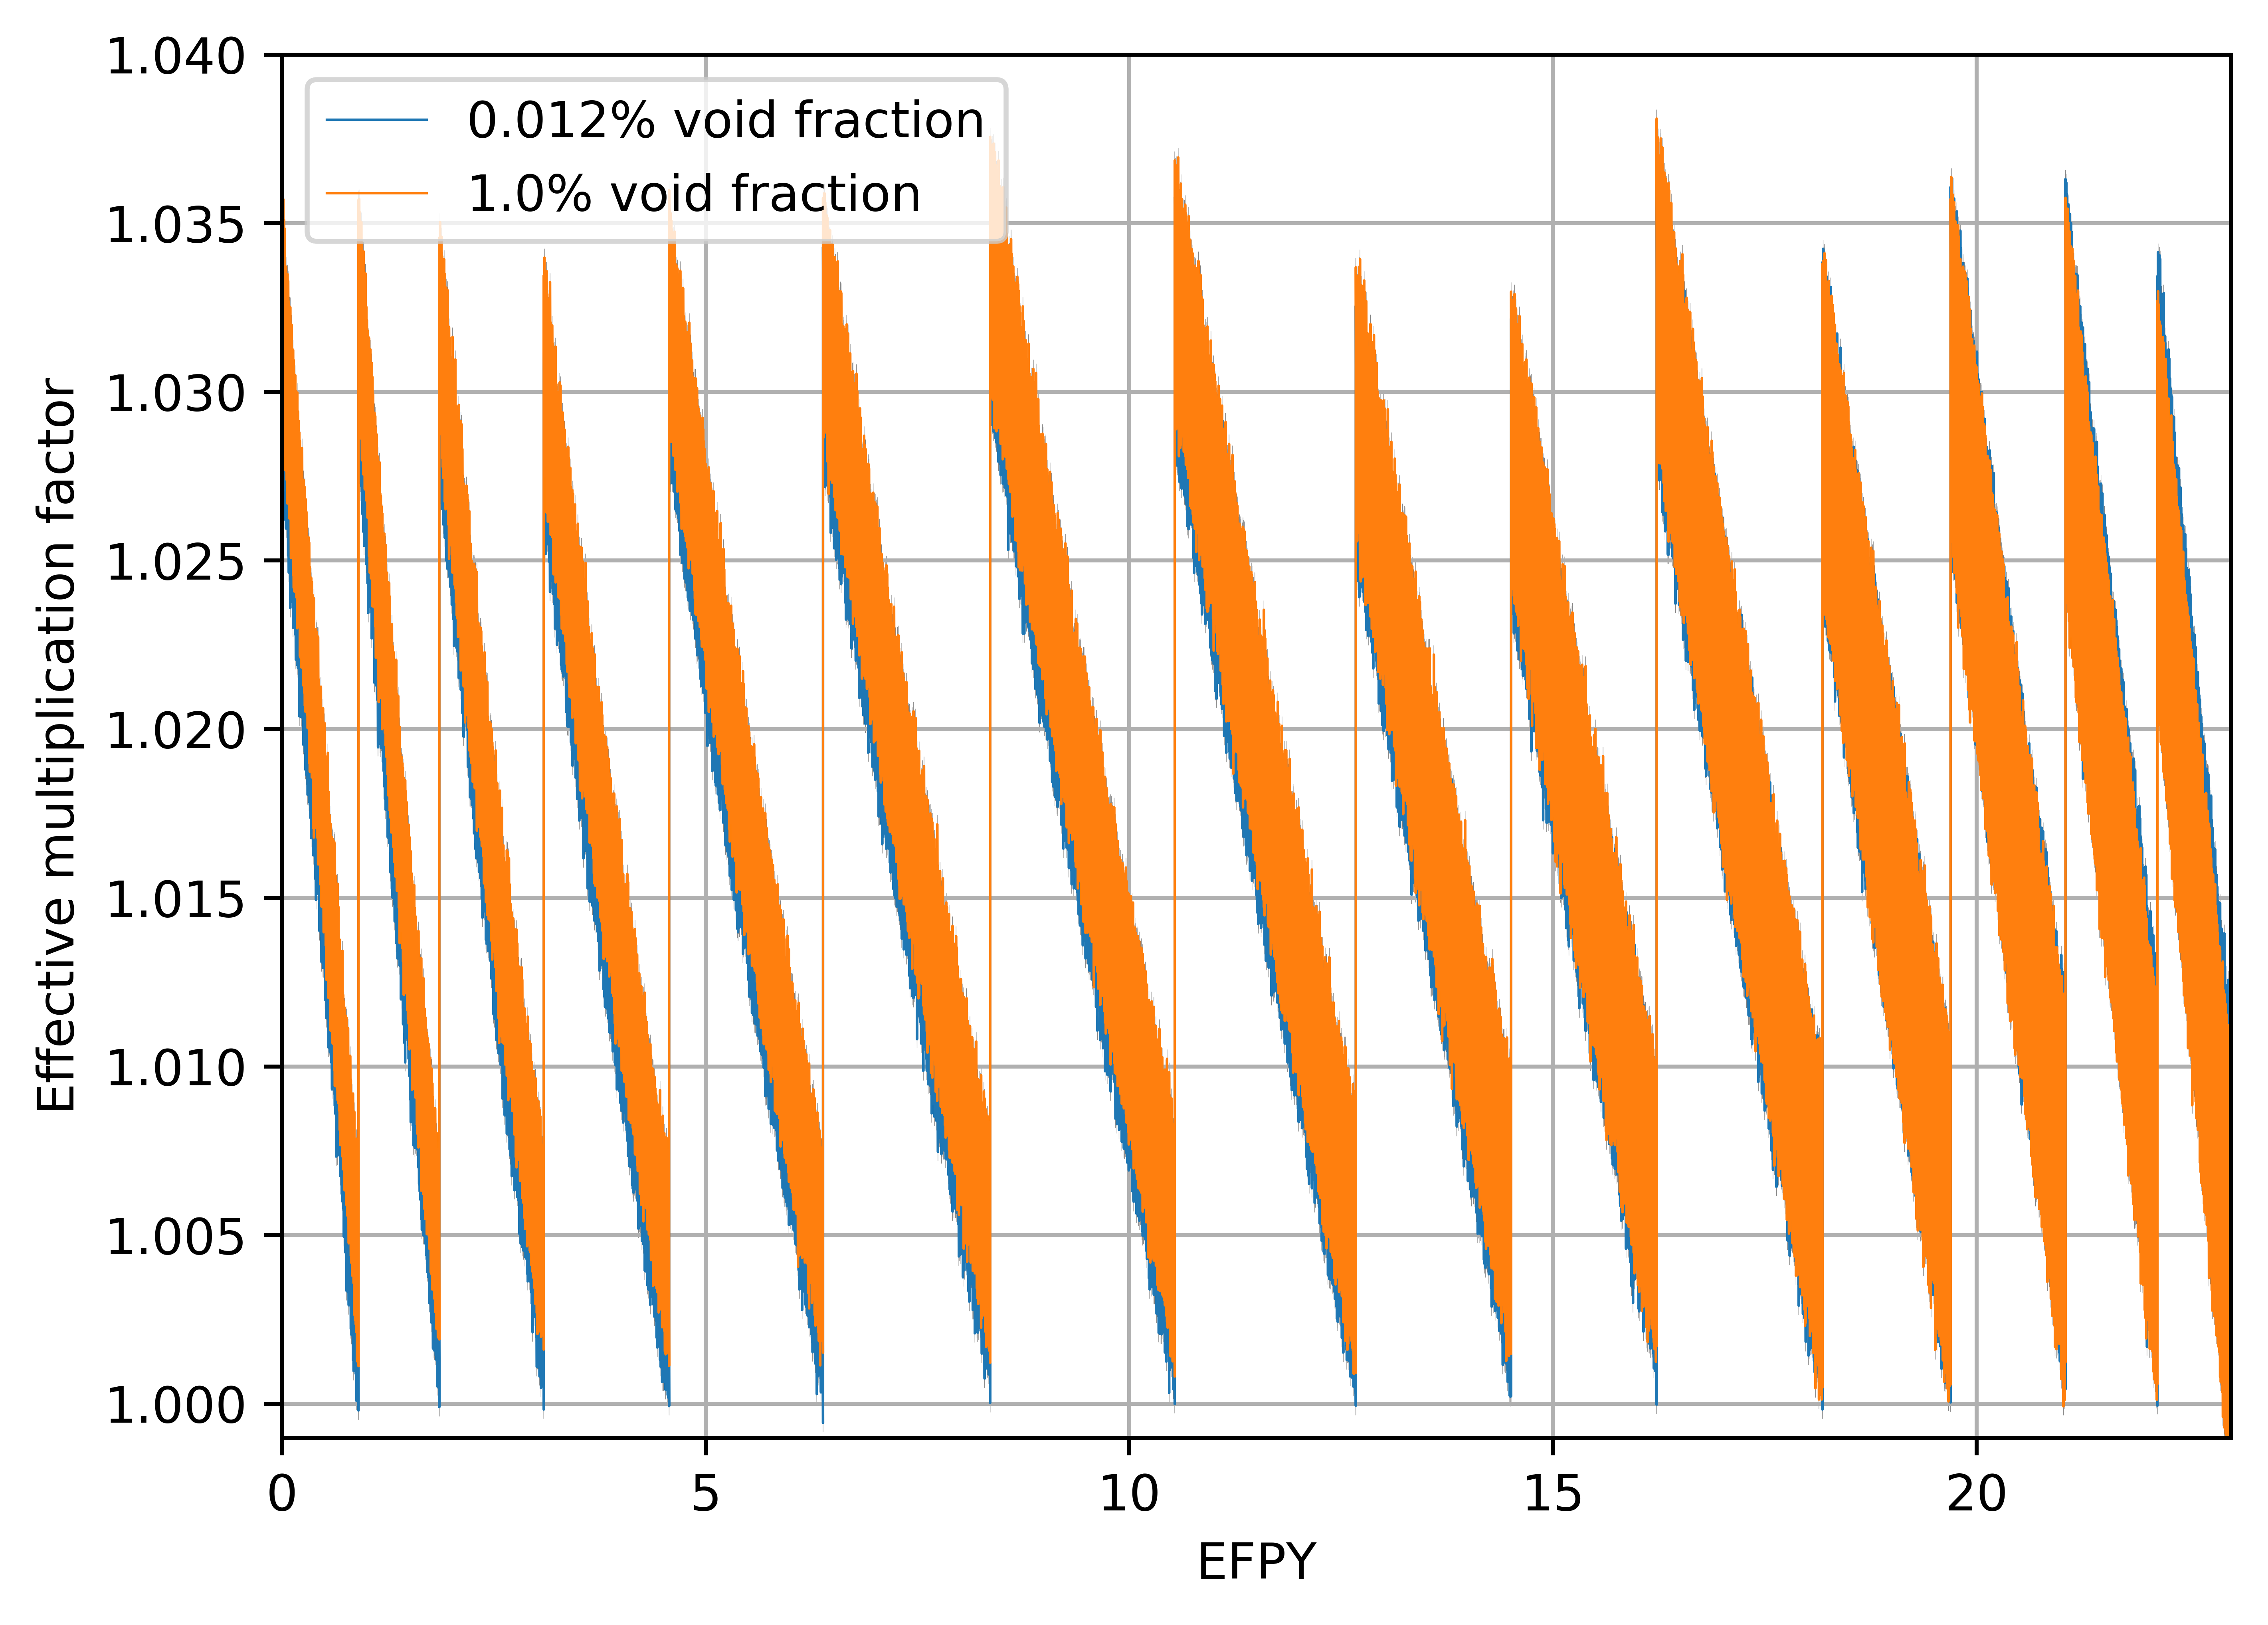
\includegraphics[width=\textwidth]{ch4/eps/keff.png}
	\caption{Effective multiplication factor dynamics for the full-core 
		\gls{TAP} core model during 25 years of operation for the case with a 
		realistic removal efficiency of fission product and various mass 
		transfer 
		coefficients. Confidence interval $\sigma=28$ $pcm$ is shaded.}
	\label{fig:keff-eps-var}
\end{figure}
\begin{figure}[htbp!] % replace 't' with 'b' to 
	\centering
	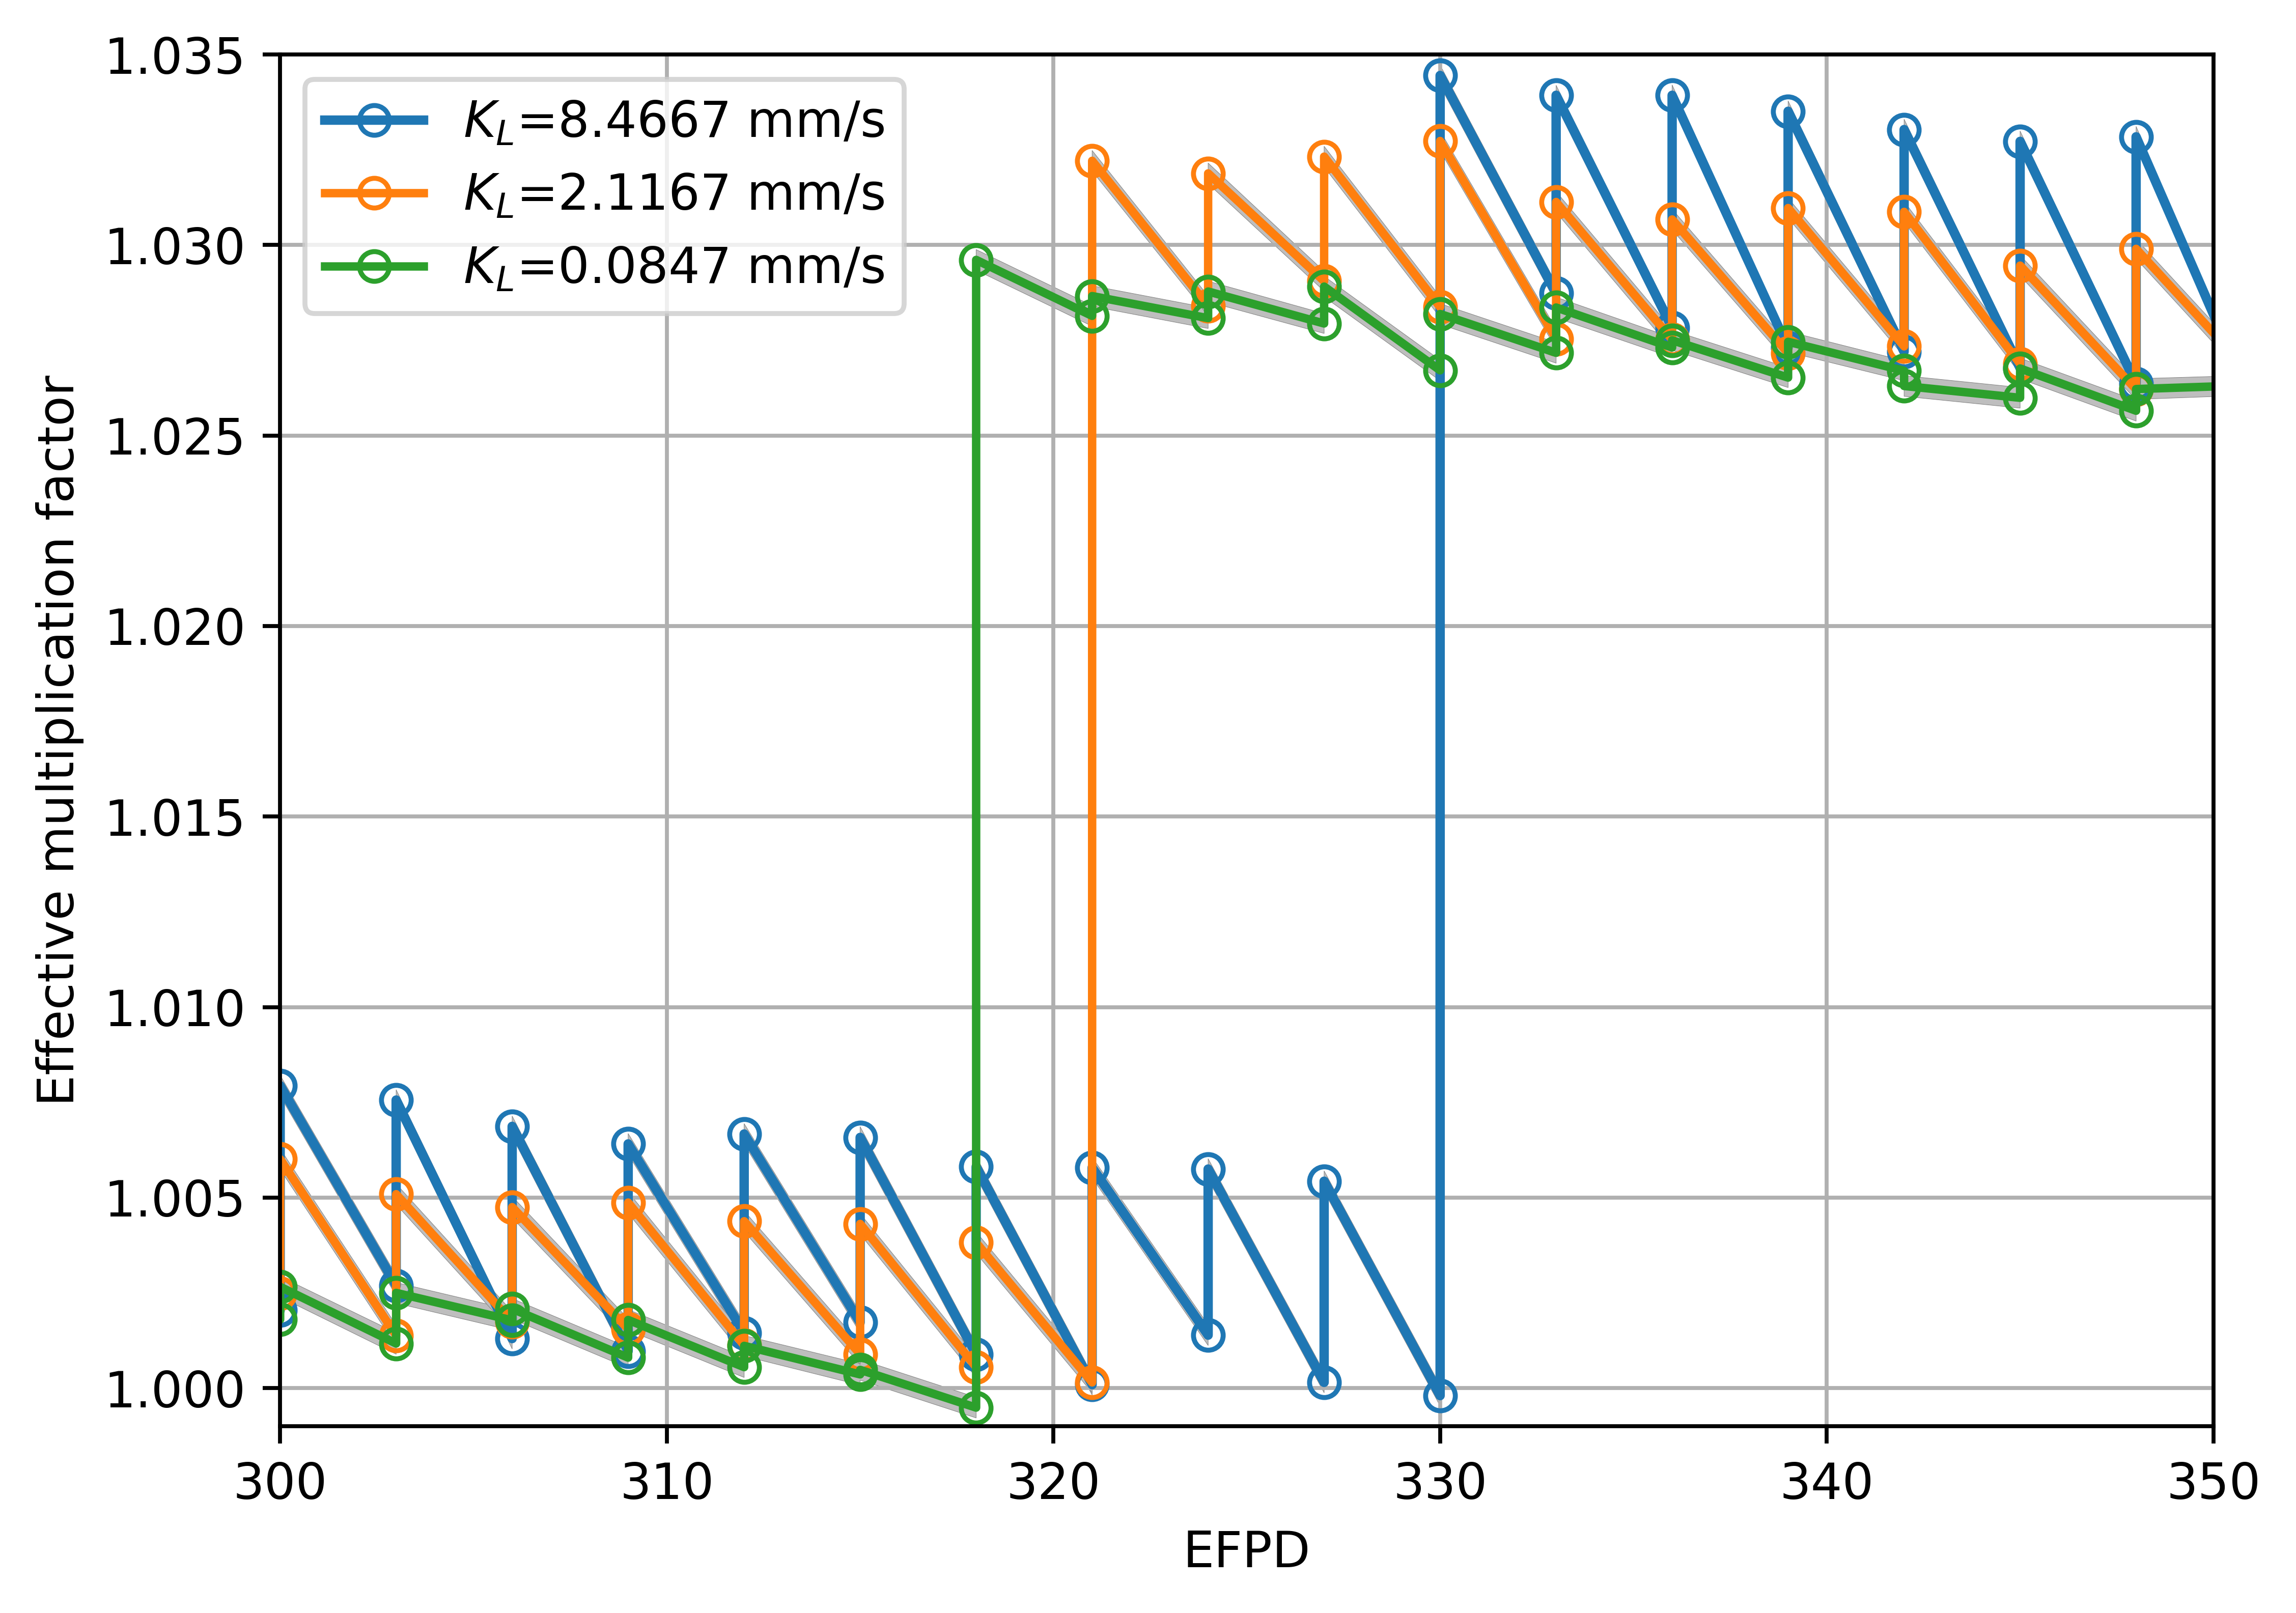
\includegraphics[width=0.93\textwidth]{ch4/eps/keff_zoomed_1.png}\\
	\vspace{-8mm}
	\hspace{+1mm}
	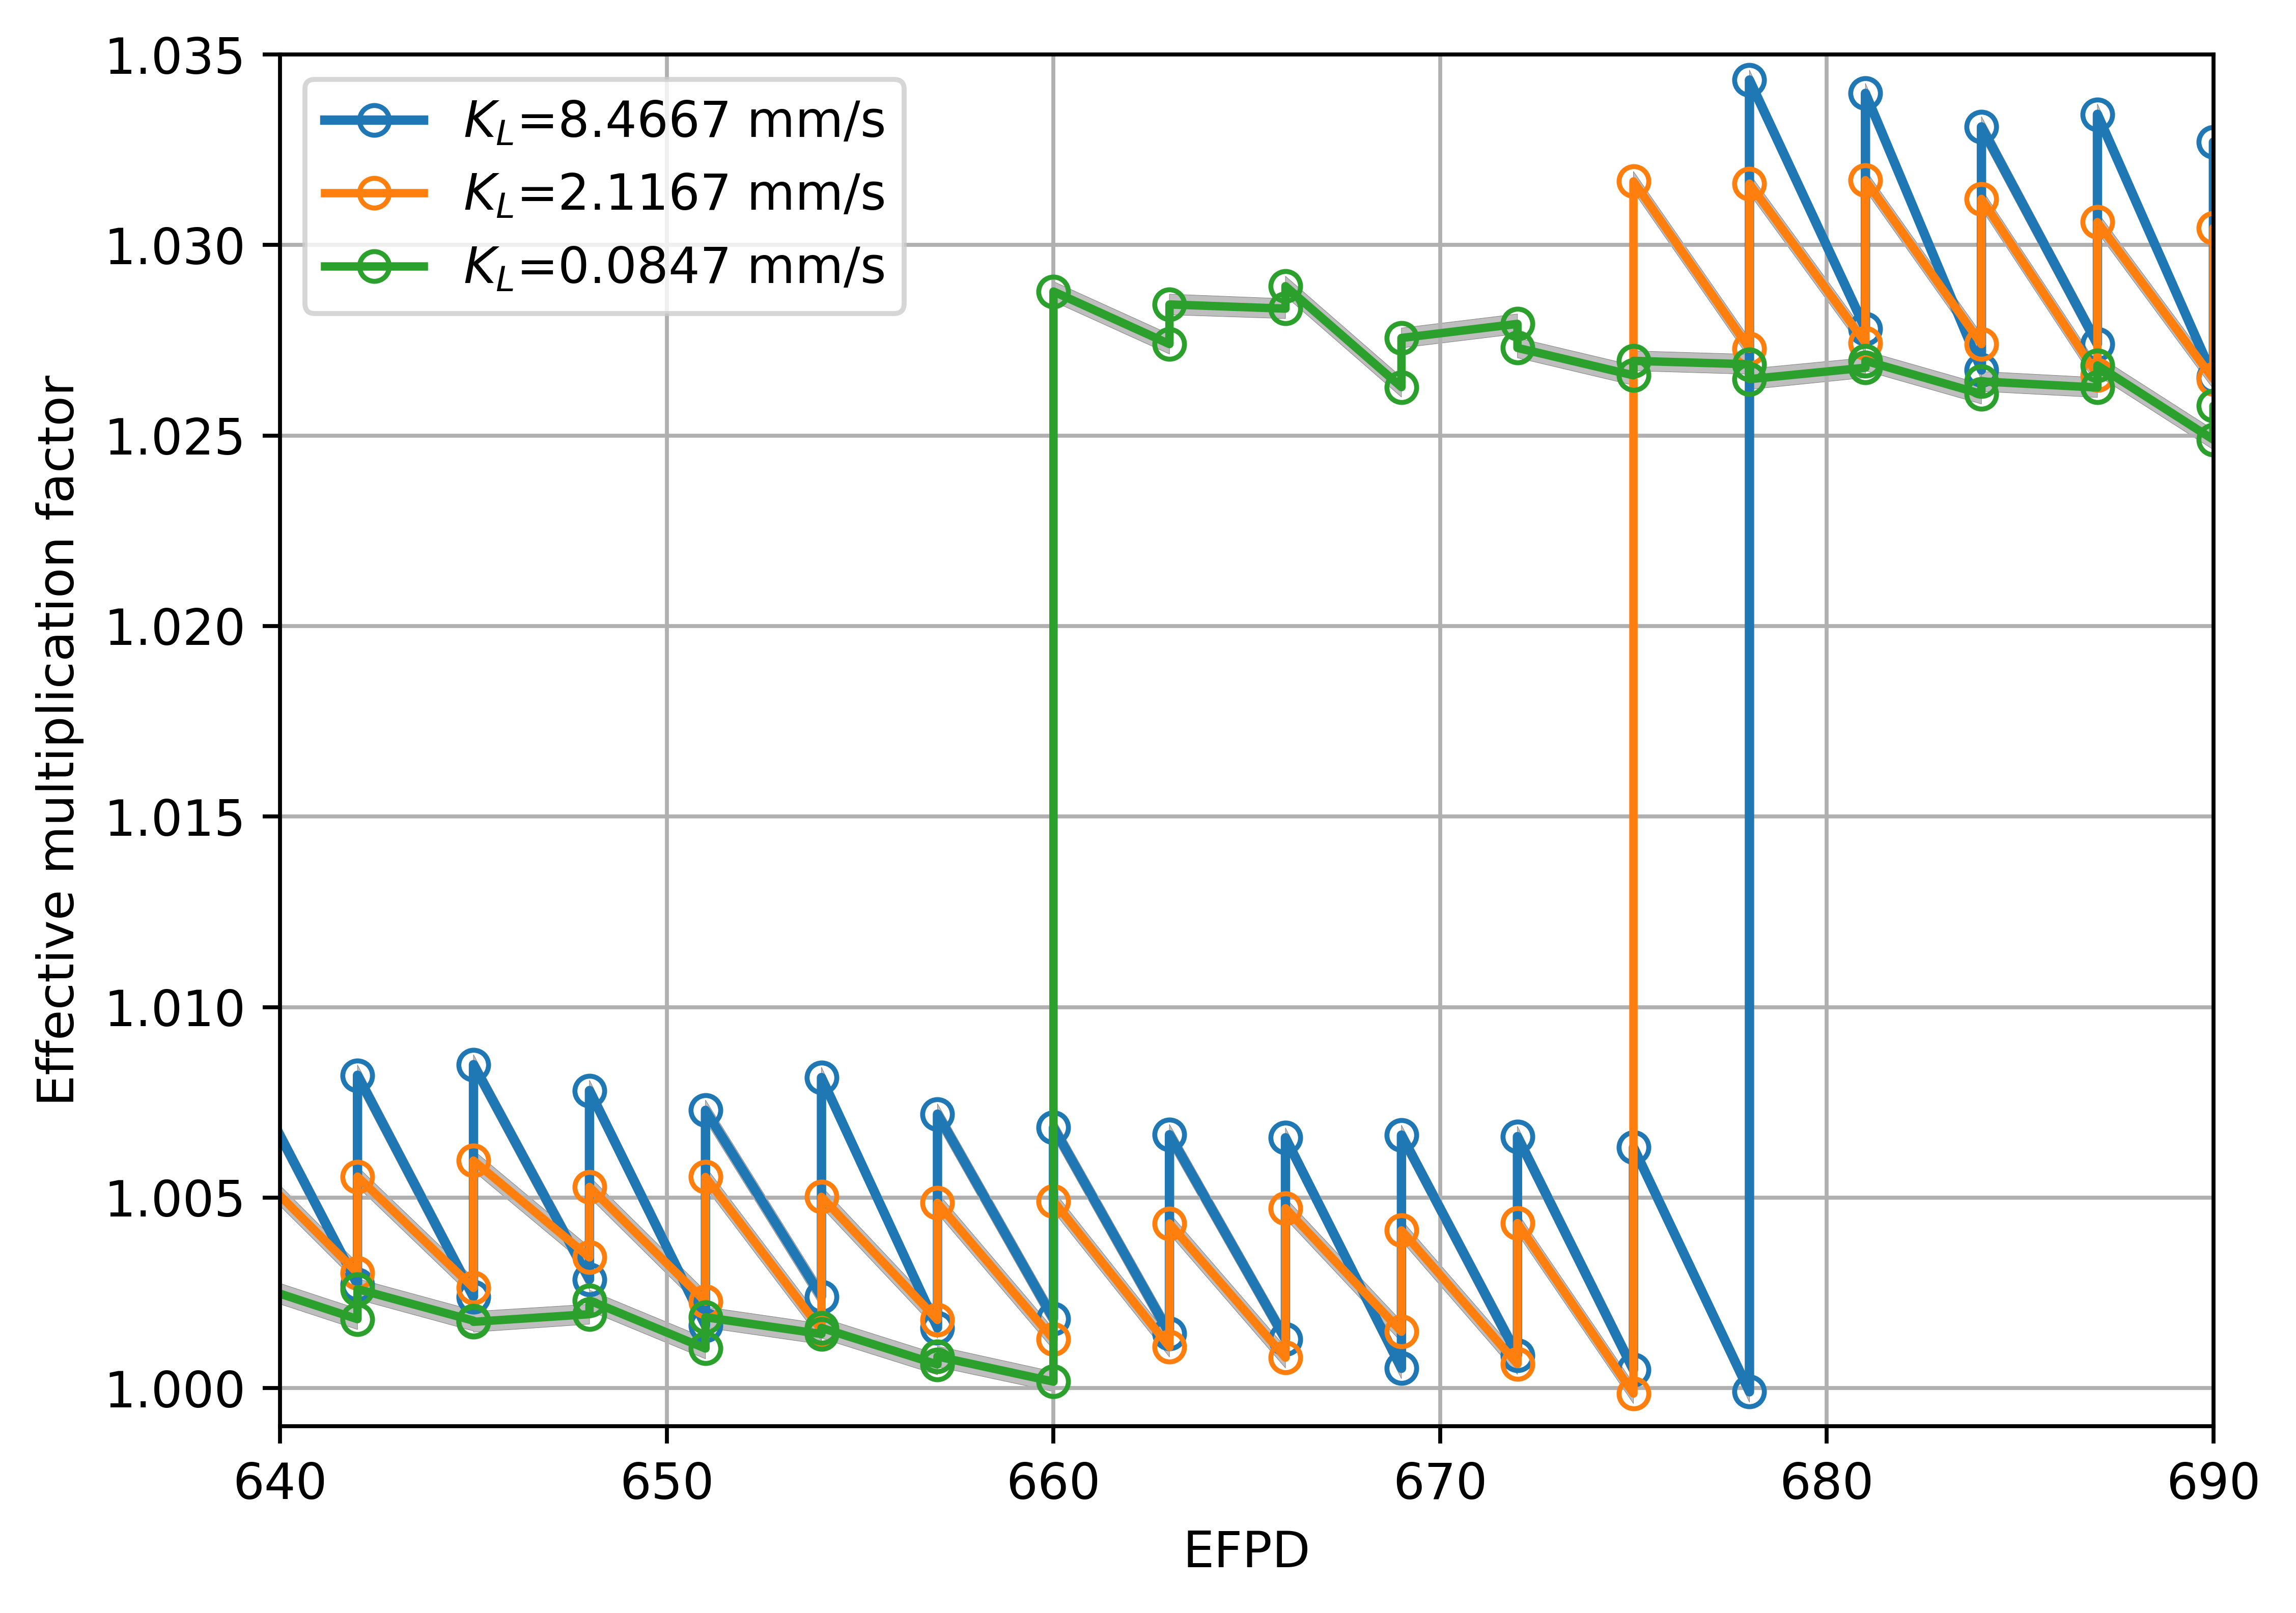
\includegraphics[width=0.93\textwidth]{ch4/eps/keff_zoomed_2.png}
	\vspace{-3mm}
	\caption{Zoomed effective multiplication factor dynamics while switching
		from Cycle \#1 (startup geometry configuration, 347 moderator rods, 
		\gls{SVF}=0.917) to Cycle \#2 (\gls{SVF}=0.887) (upper panel) and
		from Cycle \#2 to  Cycle \#3 (\gls{SVF}=0.881) 
		(lower panel) for various mass transfer coefficients ($K_L$). 
		Confidence interval $\sigma=28$ $pcm$ is shaded.}
	\label{fig:keff-eps-var-zoom}
\end{figure}

A reduced mass transfer coefficient worsens the neutron poison efficiency, 
which shortens the interval between 
shutdowns for moderator rod updates. Additionally, the presence of unremoved 
poisons in the core suppresses the effective multiplication factor after 
moderator reconfiguration ($\approx500$ $pcm$ lower for $K_L=0.0847$ $mm/s$ 
than for $K_L=8.4667$ $mm/s$ at the \gls{BOL} and $\approx1100$ $pcm$ at 
the \gls{EOL}). Overall, noble gas removal provides significant neutronics 
benefits (fewer neutrons are lost in strong absorbers such as 
$^{135}$Xe), better fuel utilization, and enables longer moderator rod 
reconfiguration intervals.

\subsubsection{Neutron spectrum}
Figure~\ref{fig:spectrum-eps-var} shows the normalized neutron flux spectrum 
for the full-core TAP core model in the energy range from 10$^{-9}$ to 15 MeV. 
The neutron energy spectrum at the \gls{EOL} is harder than at 
the \gls{BOL} due to moderator-to-fuel ratio growth during reactor operation 
caused by periodic moderator rod reconfigurations. The \gls{TAP} reactor 
spectrum is harder than in a typical \gls{LWR} and correlates well (Pearson 
correlation coefficient $>0.8$) with the \gls{TAP} neutronics white paper  
\cite{transatomic_power_corporation_neutronics_2016} and ORNL 
reports \cite{betzler_assessment_2017-1, betzler_two-dimensional_2017}.
The liquid phase mass transfer coefficient ($K_L$) and, consequently, noble 
gas removal efficiency ($\epsilon$), has a negligible effect on the spectrum 
in the fast range (between 10$^{-2}$ and 10 MeV) at the \gls{EOL}. 
\begin{figure}[htp!] % replace 't' with 'b' to 
	\centering
	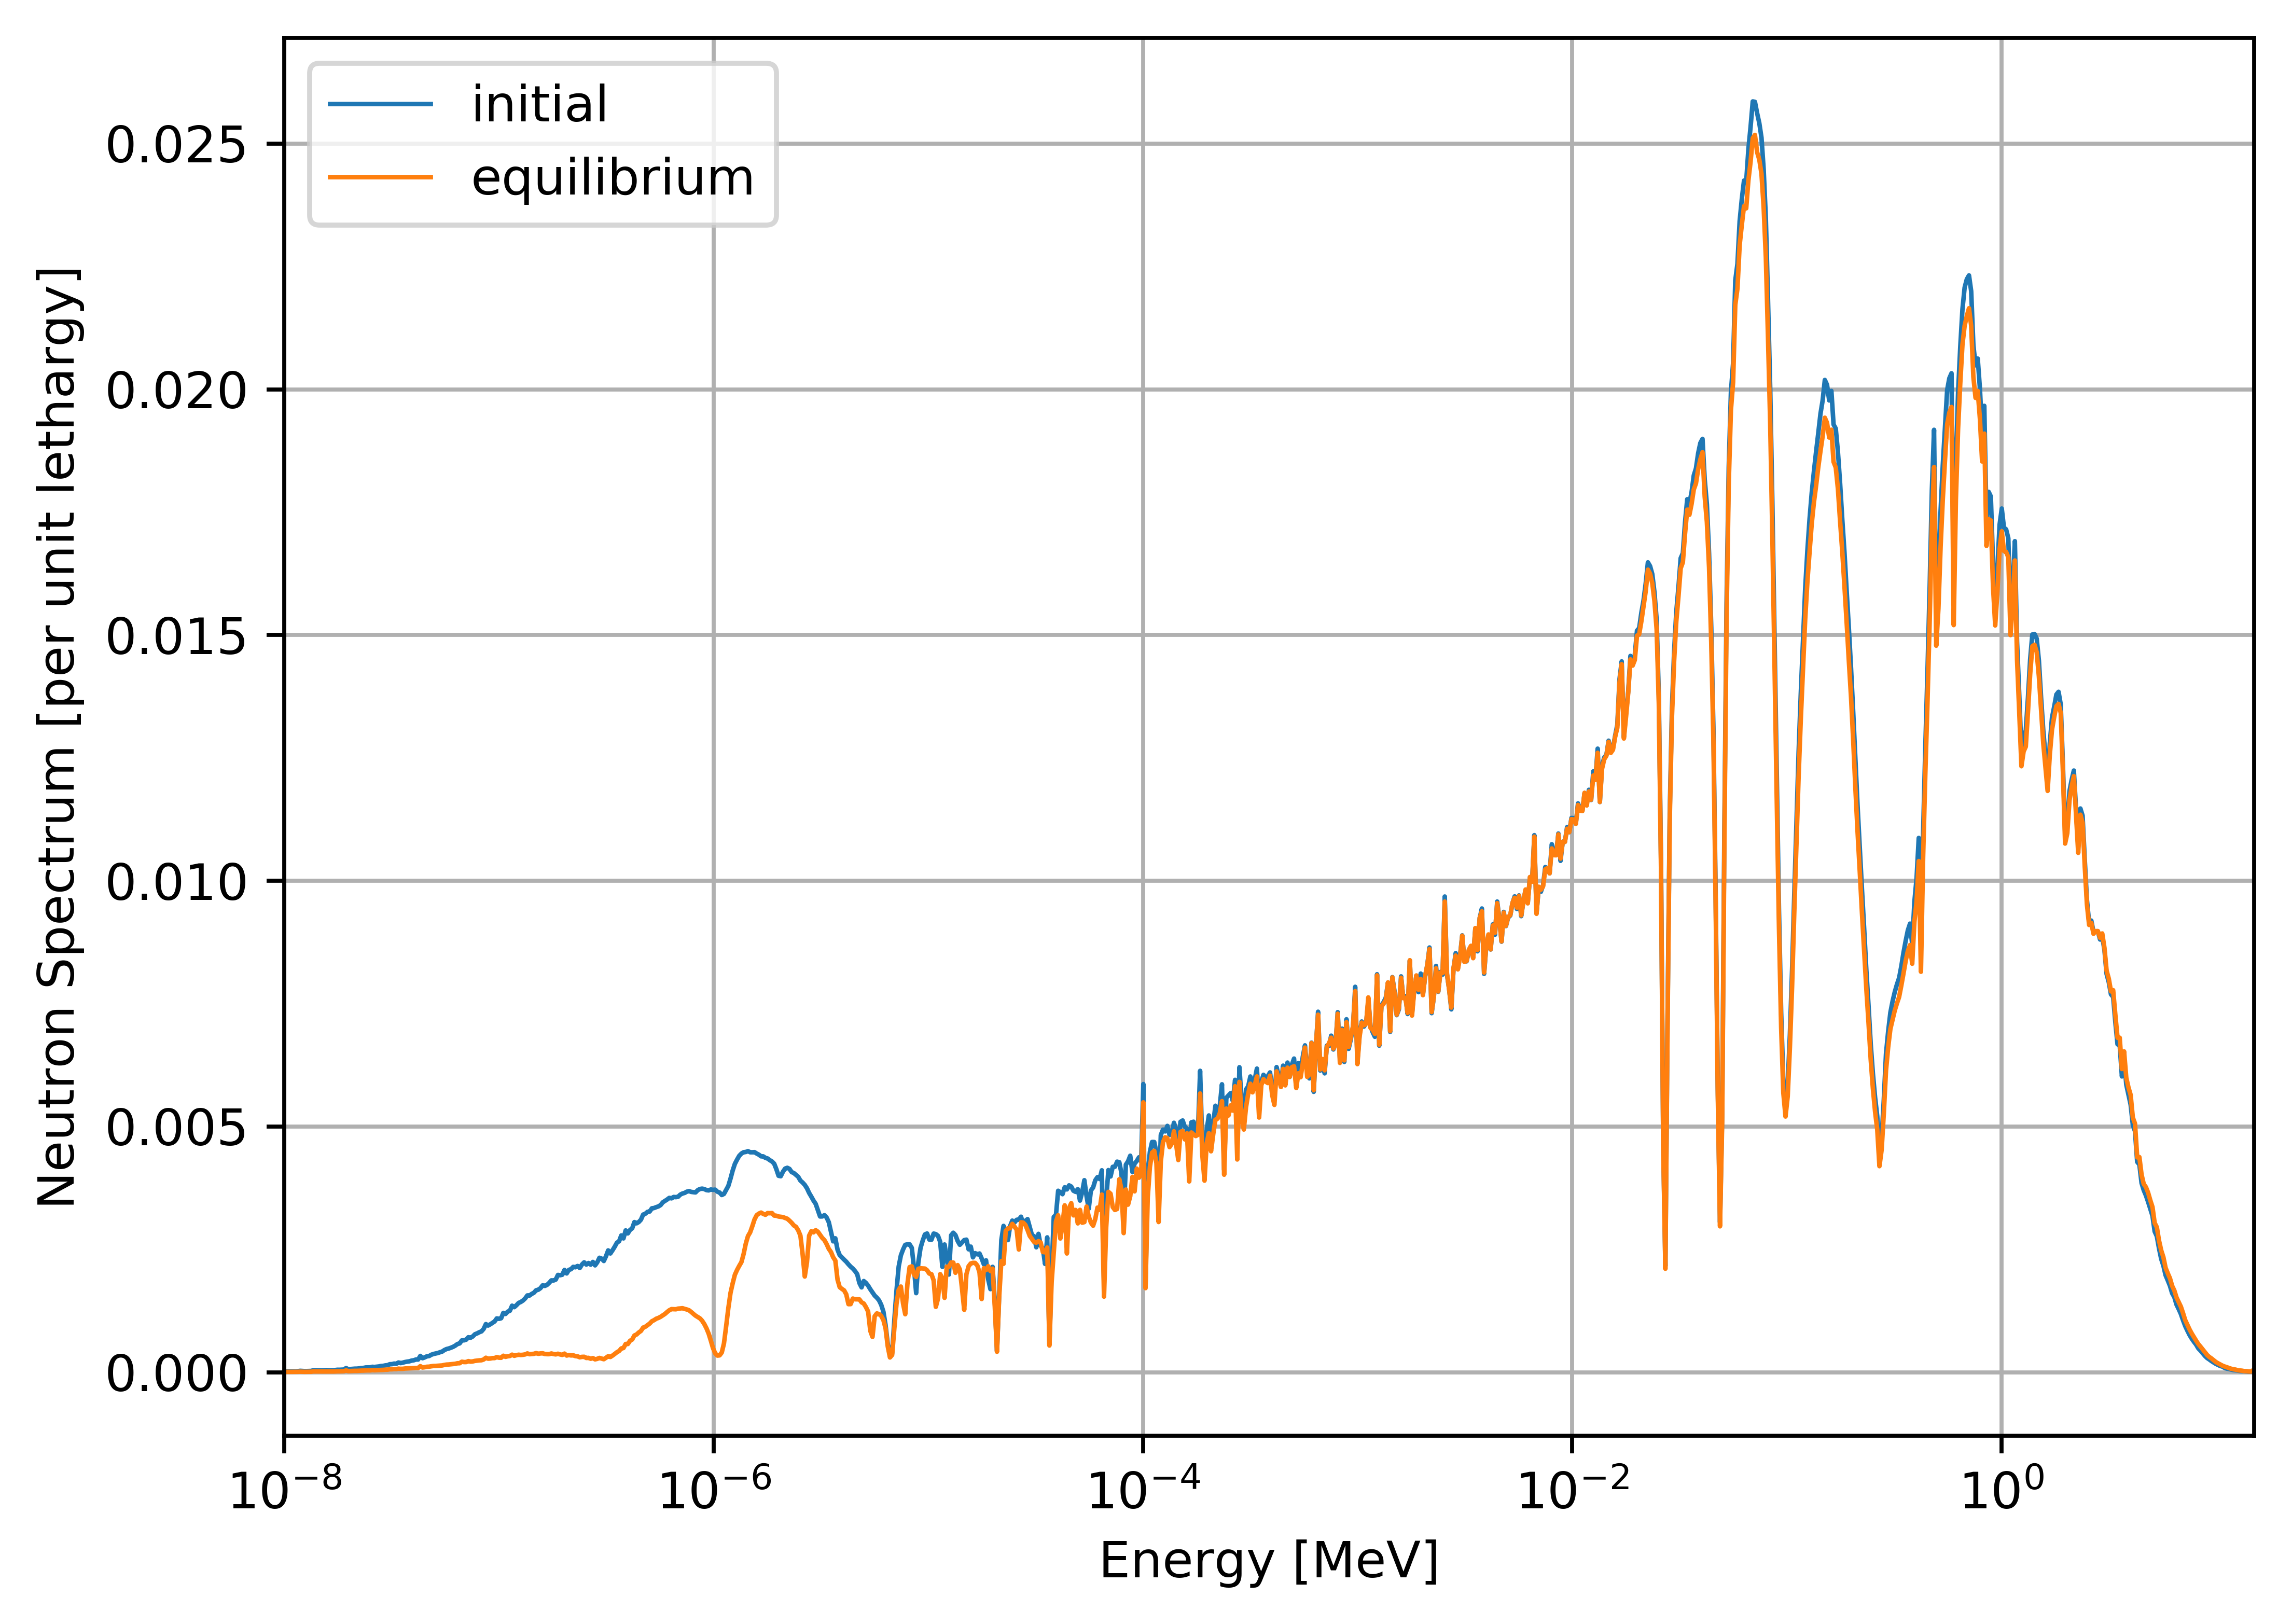
\includegraphics[width=0.7\textwidth]{ch4/eps/spectrum.png}
		\vspace{-3mm}
	\caption{The neutron flux energy spectrum normalized by unit lethargy at 
		the \gls{BOL} and \gls{EOL}	for the case with a realistic removal 
		efficiency of fission product and various mass transfer coefficients.}
	\label{fig:spectrum-eps-var}
\end{figure}

However, Figure~\ref{fig:spectrum-th-eps-var} demonstrates a notable 
difference in the thermal range of the spectrum due to the enormous $^{135}$Xe 
absorption cross section ($\sigma_{a,^{135}Xe}=2.6\times10^6$ b). 
Figure~\ref{fig:xe135-eps-var-zoomes} shows that $^{135}$Xe mass in the core 
at the \gls{EOL} for the case with low noble gas removal efficiency 
($K_L=0.0847$ $mm/s$) is significantly larger than for the case with high 
removal efficiency ($K_L=8.4667$ $mm/s$) which leads to higher neutron loss 
due to absorption in xenon. Overall, noble gas removal from the fuel salt 
alters the neutron spectrum.
\begin{figure}[htp!] % replace 't' with 'b' to 
	\centering
	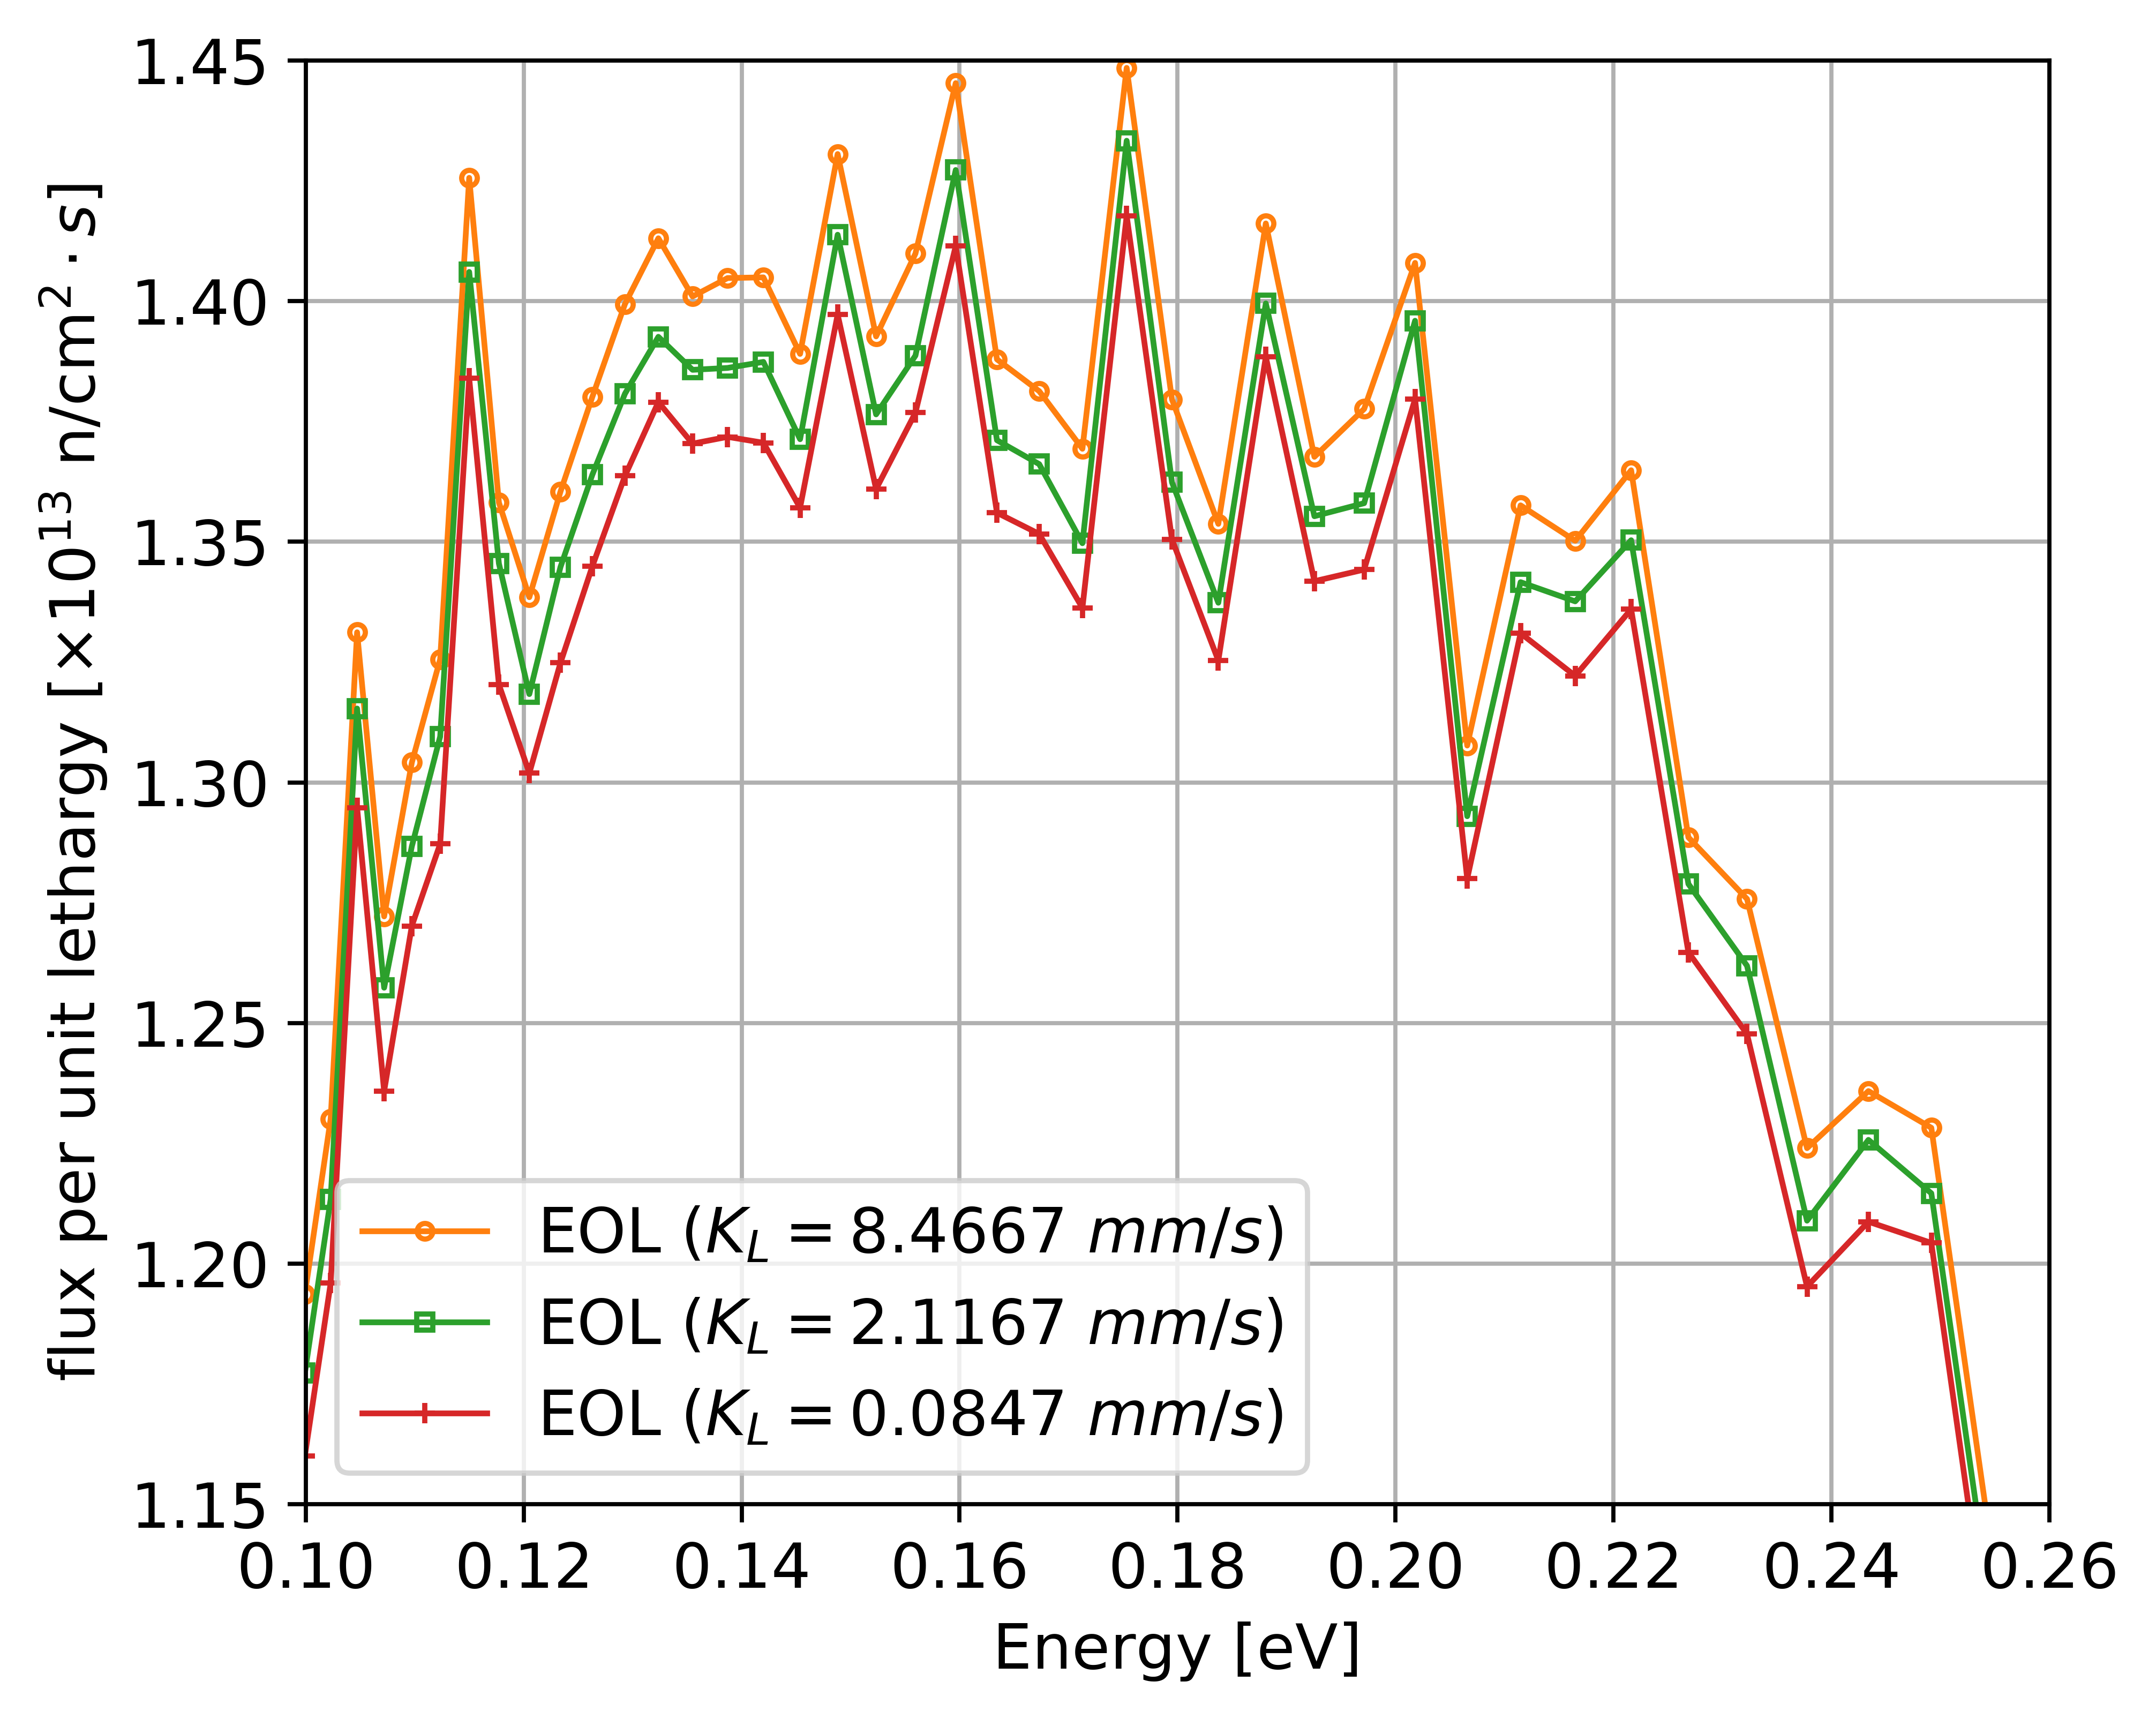
\includegraphics[width=0.7\textwidth]{ch4/eps/spectrum_th_zoomed.png}
			\vspace{-3mm}
	\caption{The neutron flux energy spectrum normalized by unit lethargy  
		\gls{EOL} zoomed in the thermal energy range.}
	\label{fig:spectrum-th-eps-var}
\end{figure}


\subsubsection{Fuel salt isotopic composition evolution}
The time-dependent isotopic compositions obtained with different noble gas 
extraction efficiencies behave very similarly. For $^{235}$U predicted mass, 
the difference between $K_L=8.4667$ $mm/s$ (e.g., 91.5\% of $^{135}$Xe is 
removed) and $K_L=0.0847$ $mm/s$ (e.g., 3.1\% of $^{135}$Xe is removed) is 
within 0.2\% for 
the first 14 years and rises rapidly to 1.15\% over the remaining 10 years  
(Figure~\ref{fig:u235-eps-var}). The simulations with a mass transfer  
coefficient smaller than $8.4467$ $mm/s$ retain more
$^{235}$U during operation because more neutrons are parasitically 
absorbed by the noble gas, which leads to a lower fission rate. The 
relative mass difference in $^{238}$U is small 
(Figure~\ref{fig:u238-eps-var}), but the absolute difference is approximately 
50 kg at the \gls{EOL}, with low removal efficiency corresponding to a reduced 
\gls{EOL} inventory of $^{235}$U.
\begin{figure}[htp!] % replace 't' with 'b' to 
	\centering
	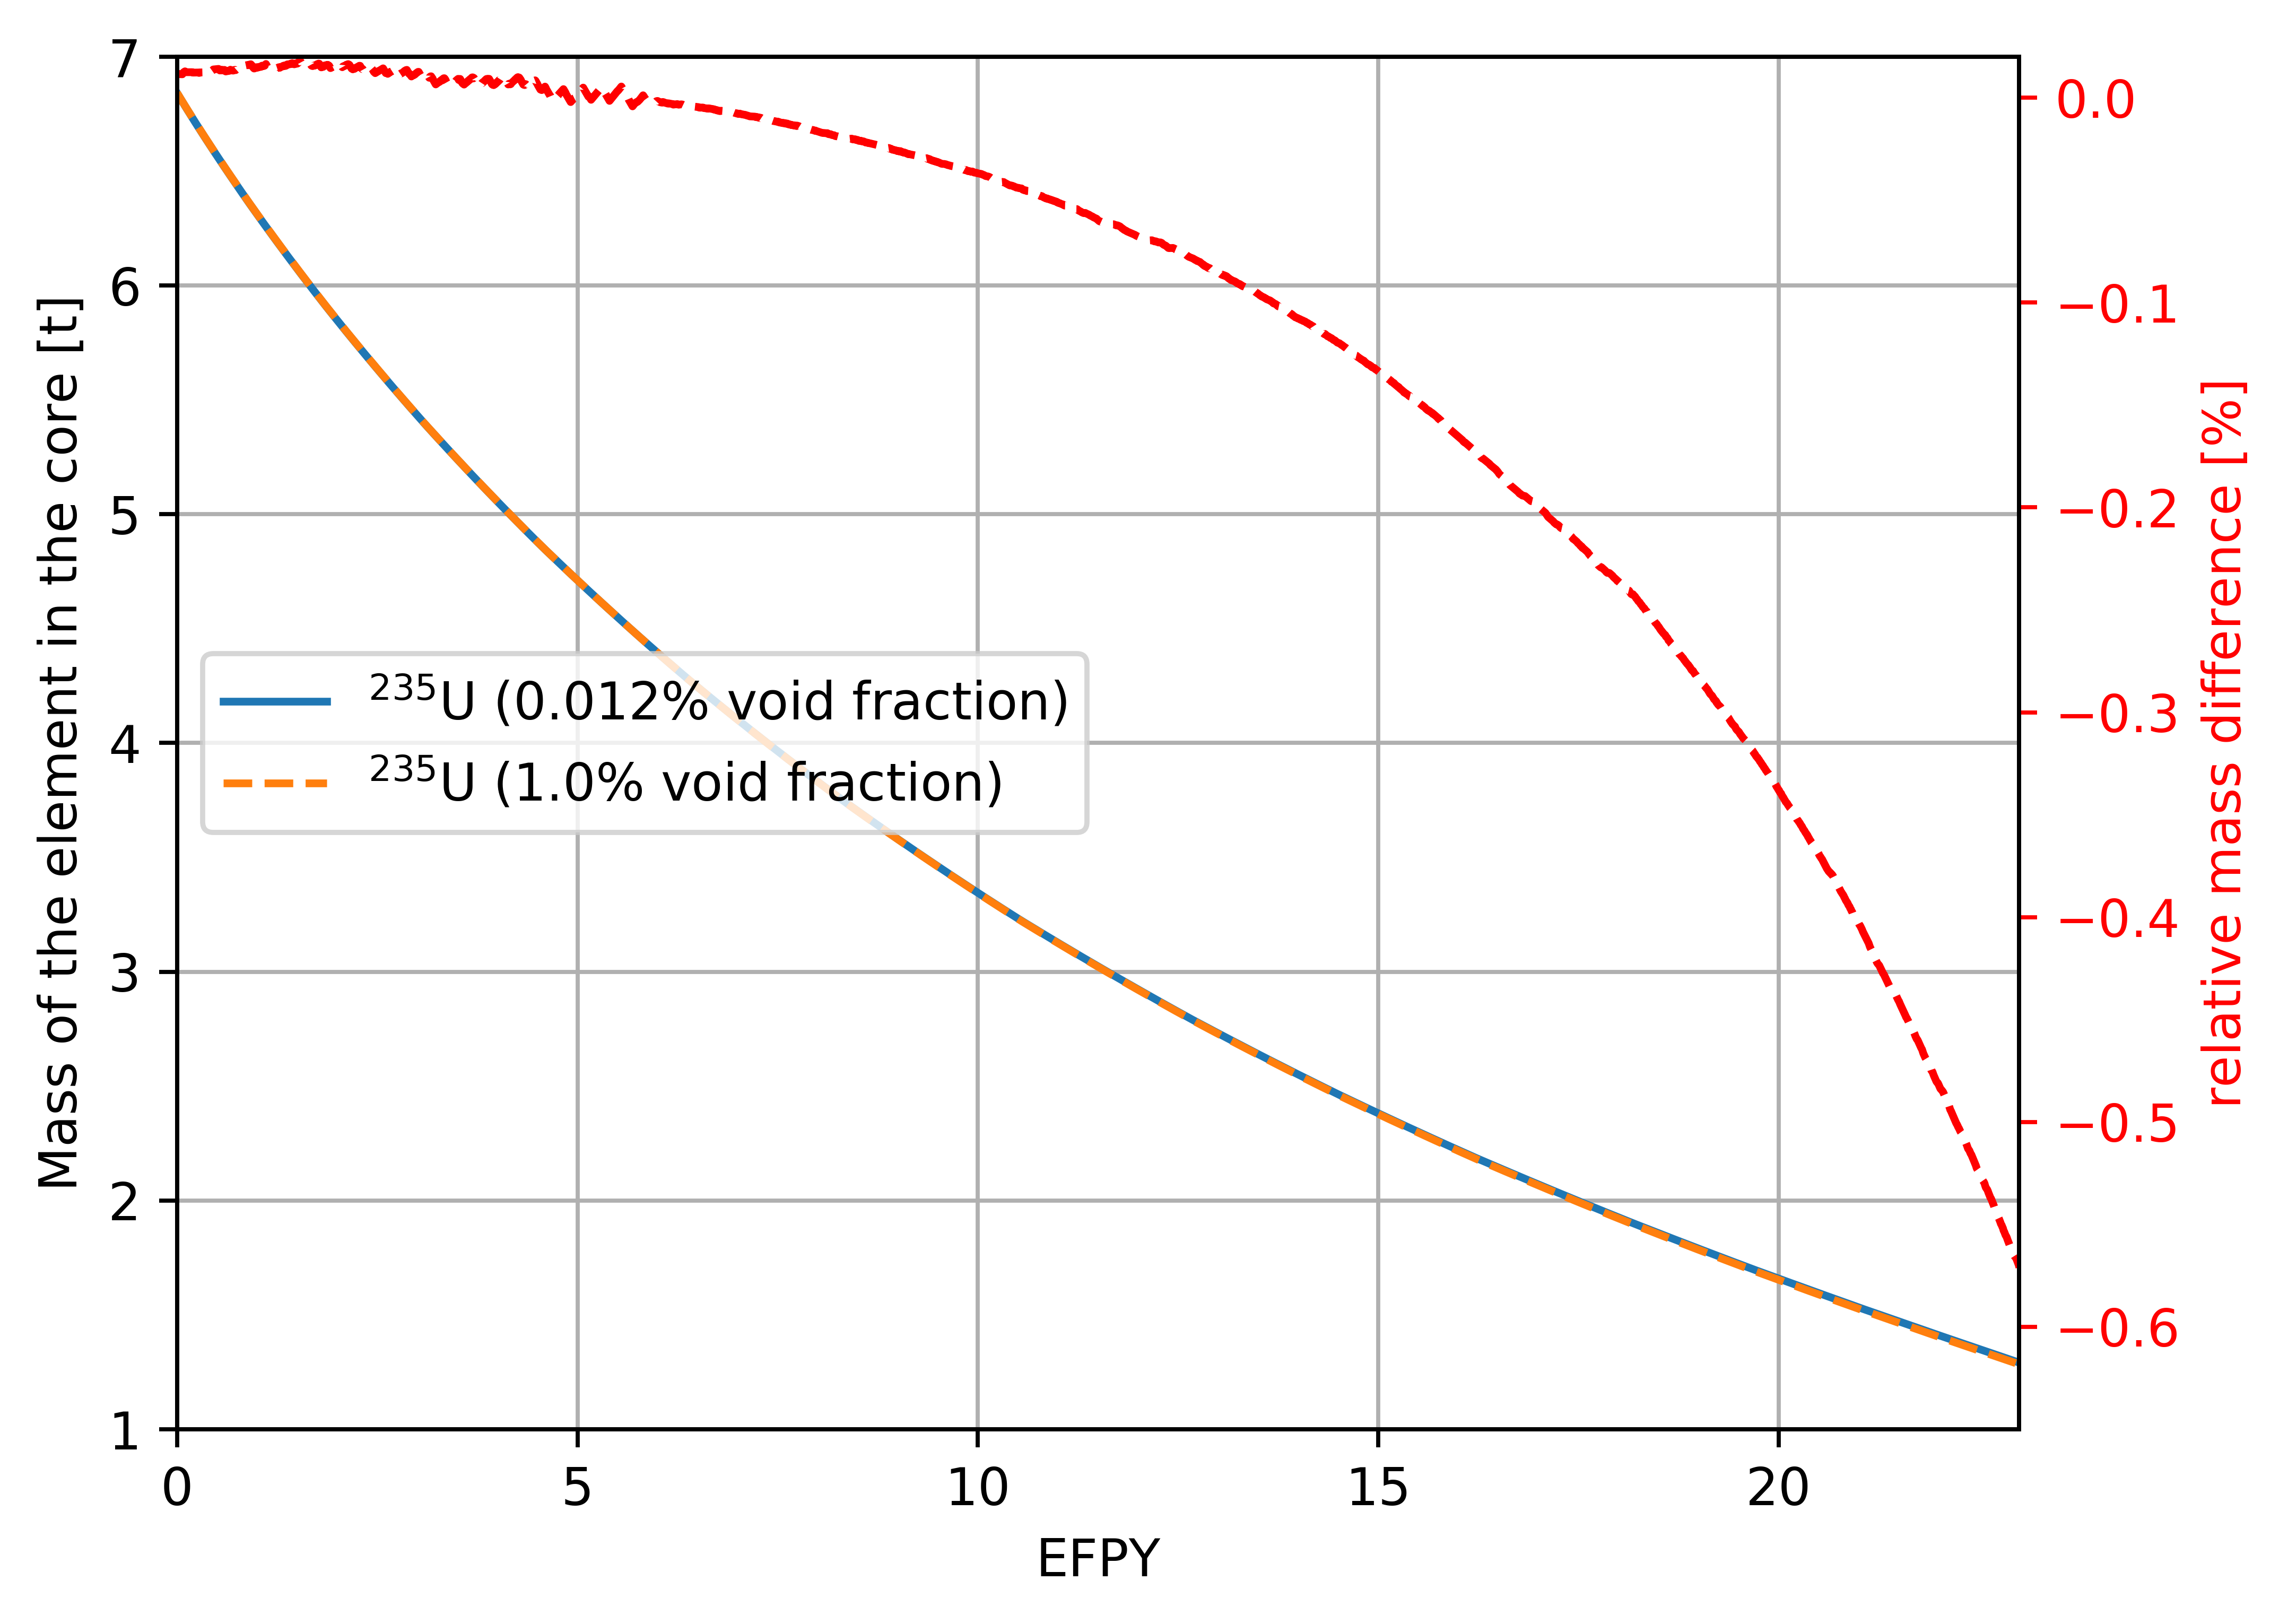
\includegraphics[width=0.8\textwidth]{ch4/eps/u235.png}
		\vspace{-4mm}
	\caption{SaltProc-calculated mass of $^{235}$U in the fuel salt during 
		25 years of operation for $K_L=8.4667$ $mm/s$ compared with less 
		effective noble gas removal.}
	\label{fig:u235-eps-var}
\end{figure}
\begin{figure}[hbp!] % replace 't' with 'b' to 
	\centering
	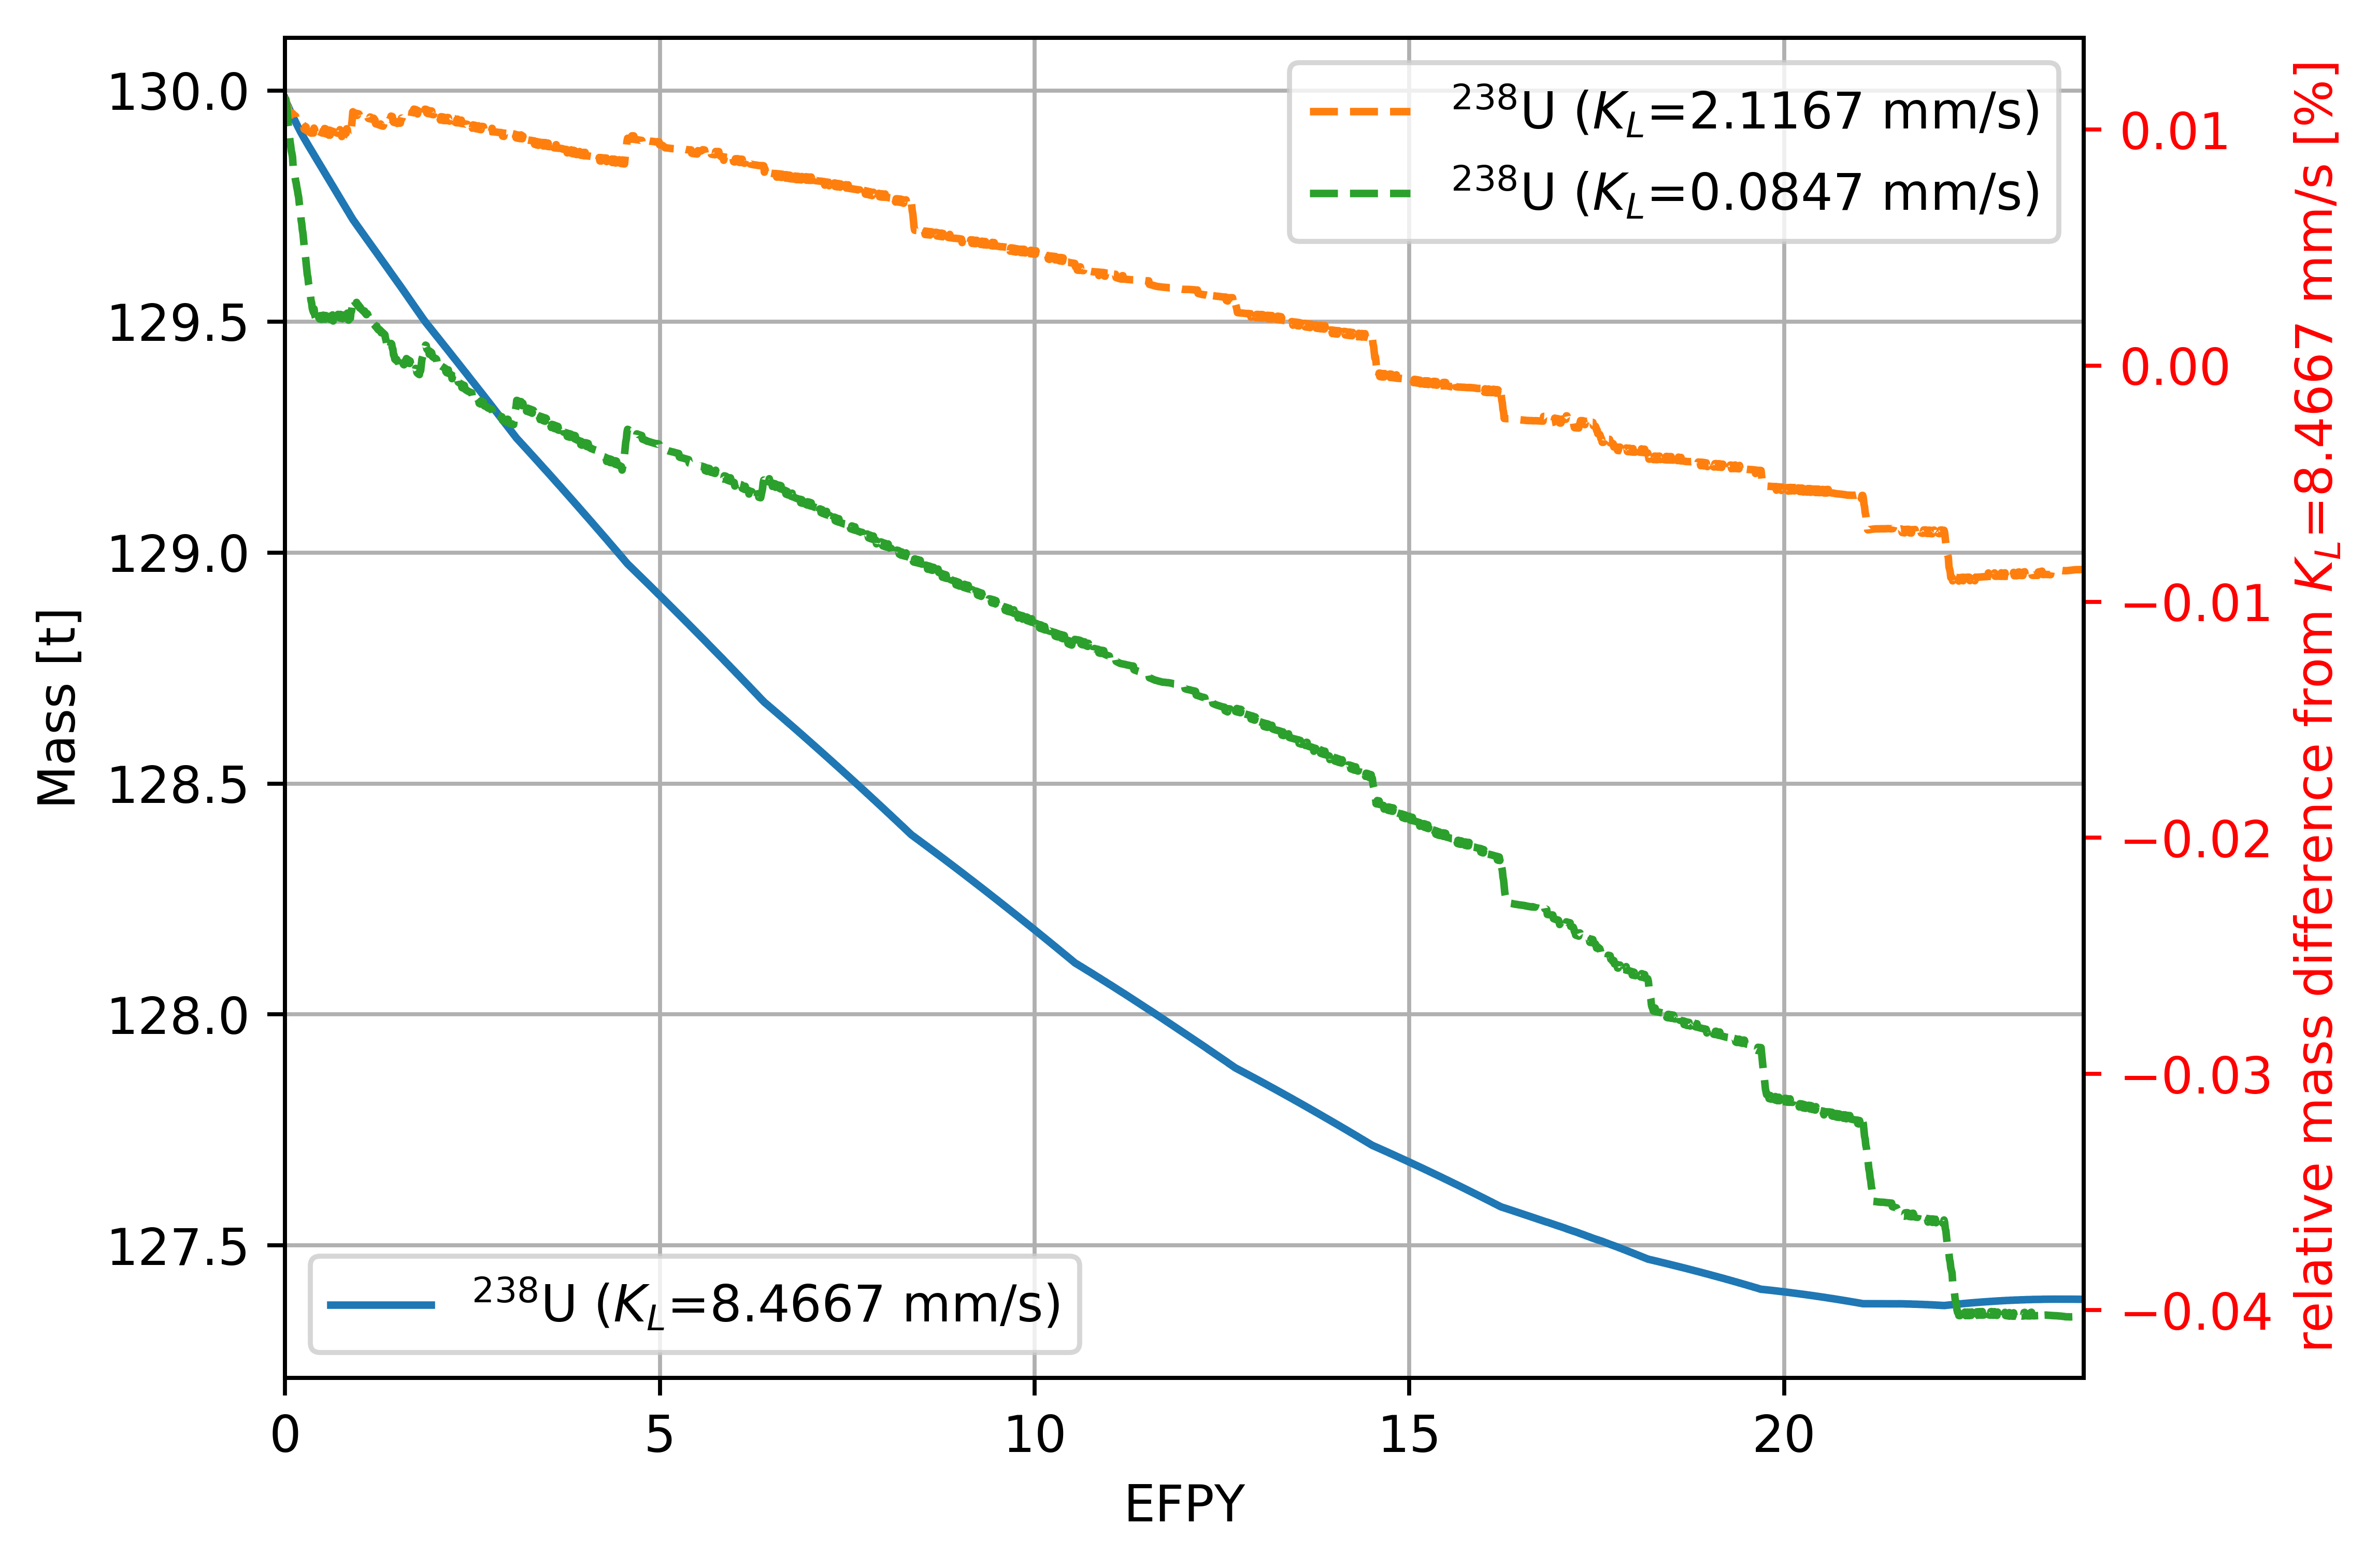
\includegraphics[width=0.85\textwidth]{ch4/eps/u238.png}
		\vspace{-4mm}
	\caption{SaltProc-calculated mass of $^{238}$U in the fuel salt during 
		25 years of operation for $K_L=8.4667$ $mm/s$ compared with less 
		effective noble gas removal.}
	\label{fig:u238-eps-var}
\end{figure}

Differences in the plutonium production between cases with different gas 
removal efficiencies are much greater. Over 3\% more $^{239}$Pu mass is 
generated in 
the case with $K_L=0.0847$ $mm/s$ than with $K_L=8.4667$ $mm/s$ 
(Figure~\ref{fig:pu239-eps-var}). The greater mass of neutron poison 
($^{135}$Xe) in the core leads to a harder spectrum 
(Figure~\ref{fig:spectrum-th-eps-var}), which results in a faster rate of 
destruction of $^{238}$U and increased breeding of fissile $^{239}$Pu.
\begin{figure}[hbp!] % replace 't' with 'b' to 
	\centering
	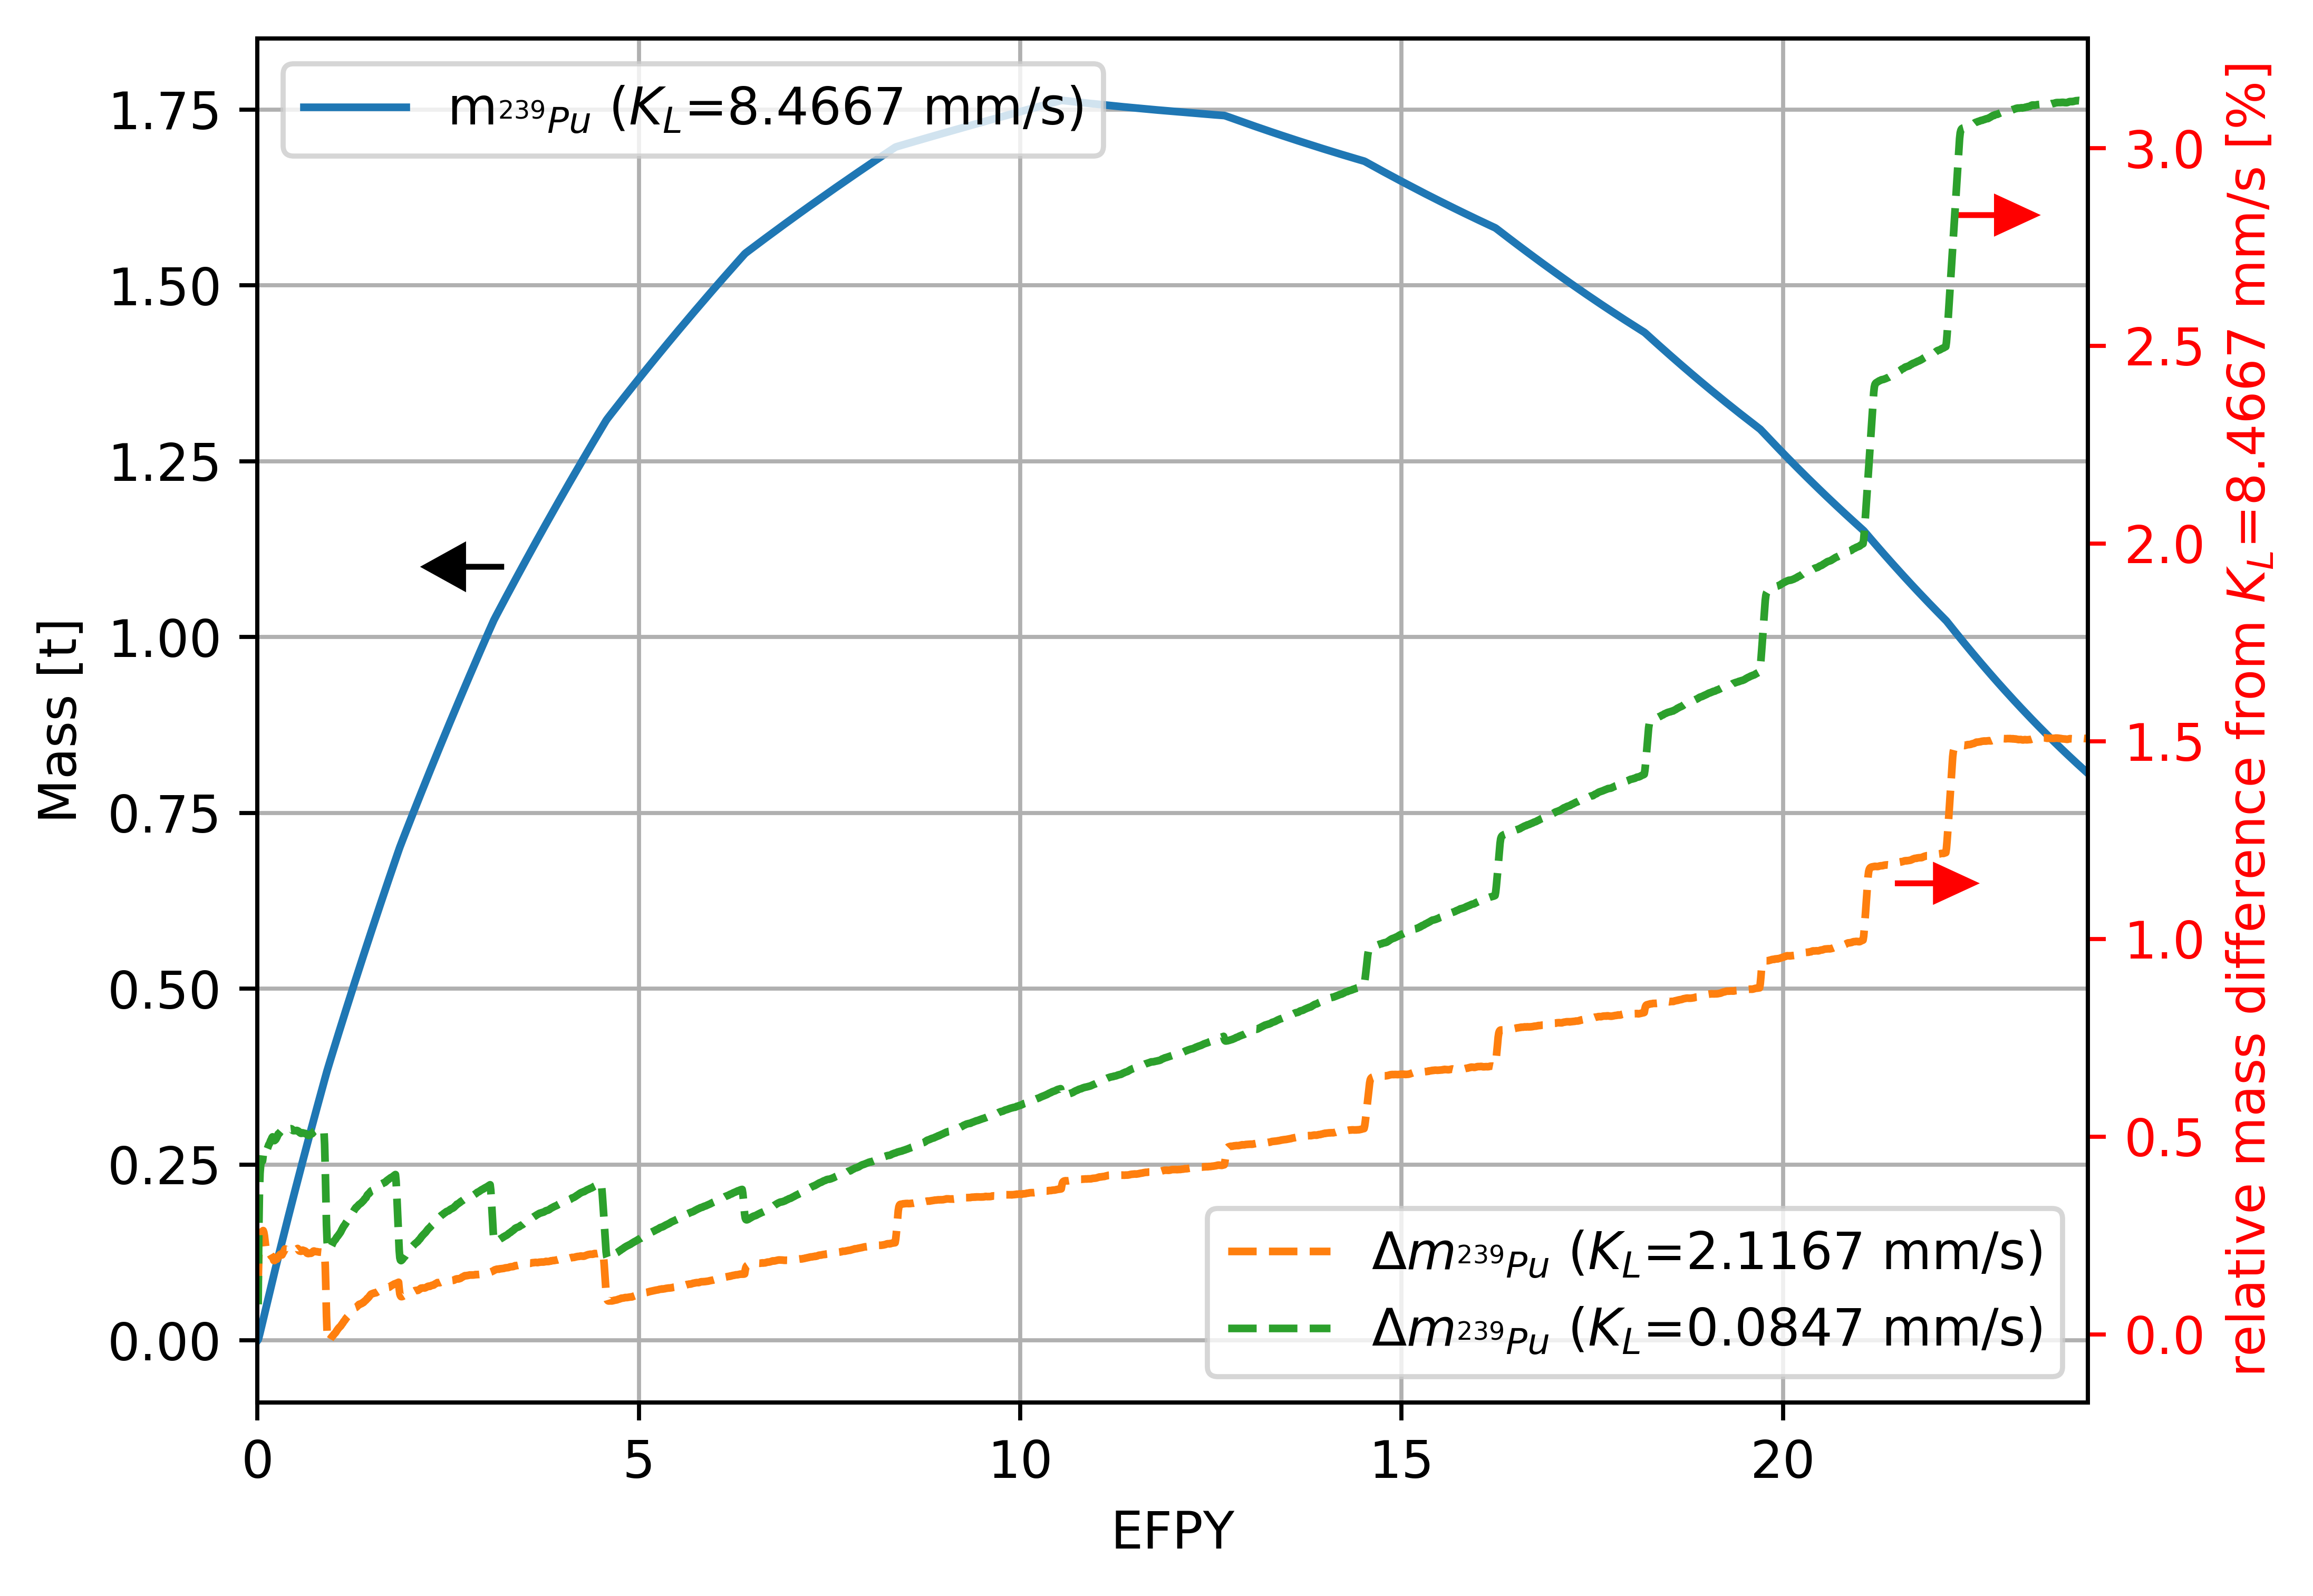
\includegraphics[width=0.8\textwidth]{ch4/eps/pu239.png}
	\caption{SaltProc-calculated mass of $^{239}$Pu in the fuel salt during 
		25 years of operation for $K_L=8.4667$ $mm/s$ (91.5\% of $^{135}$Xe is 
		removed) compared with less effective noble gas removal.}
	\label{fig:pu239-eps-var}
\end{figure}


Figure~\ref{fig:xe135-eps-var} demonstrates $^{135}$Xe mass dynamics in the 
\gls{TAP} core during 25 years of operation for various mass transfer 
coefficients. Jumps in $^{135}$Xe mass every few years reflect the 
spectral shifts due to moderator rod reconfiguration. In 
contrast, the mass of $^{135}$I, which is the primary direct precursor of 
$^{135}$Xe, is approximately 18 g and stays almost constant over 25 years.

Figure~\ref{fig:xe135-eps-var-zoomes} shows $^{135}$Xe mass at the 
end of each depletion time step before and after performing the fuel salt 
reprocessing procedure in SaltProc v1.0. $^{135}$Xe concentration in the core 
after performing \gls{FP} removals behaves as expected and is consistent with 
calculated extraction efficiencies in Table~\ref{tab:gas_removal_efficiency}.
Notably, the $^{135}$Xe production rate increases during the first seven years 
of operation and then decreases rapidly to 17 g during  the remaining 17 years 
as the spectrum thermalizes during operation.

\begin{figure}[htp!] % replace 't' with 'b' to 
	\centering
	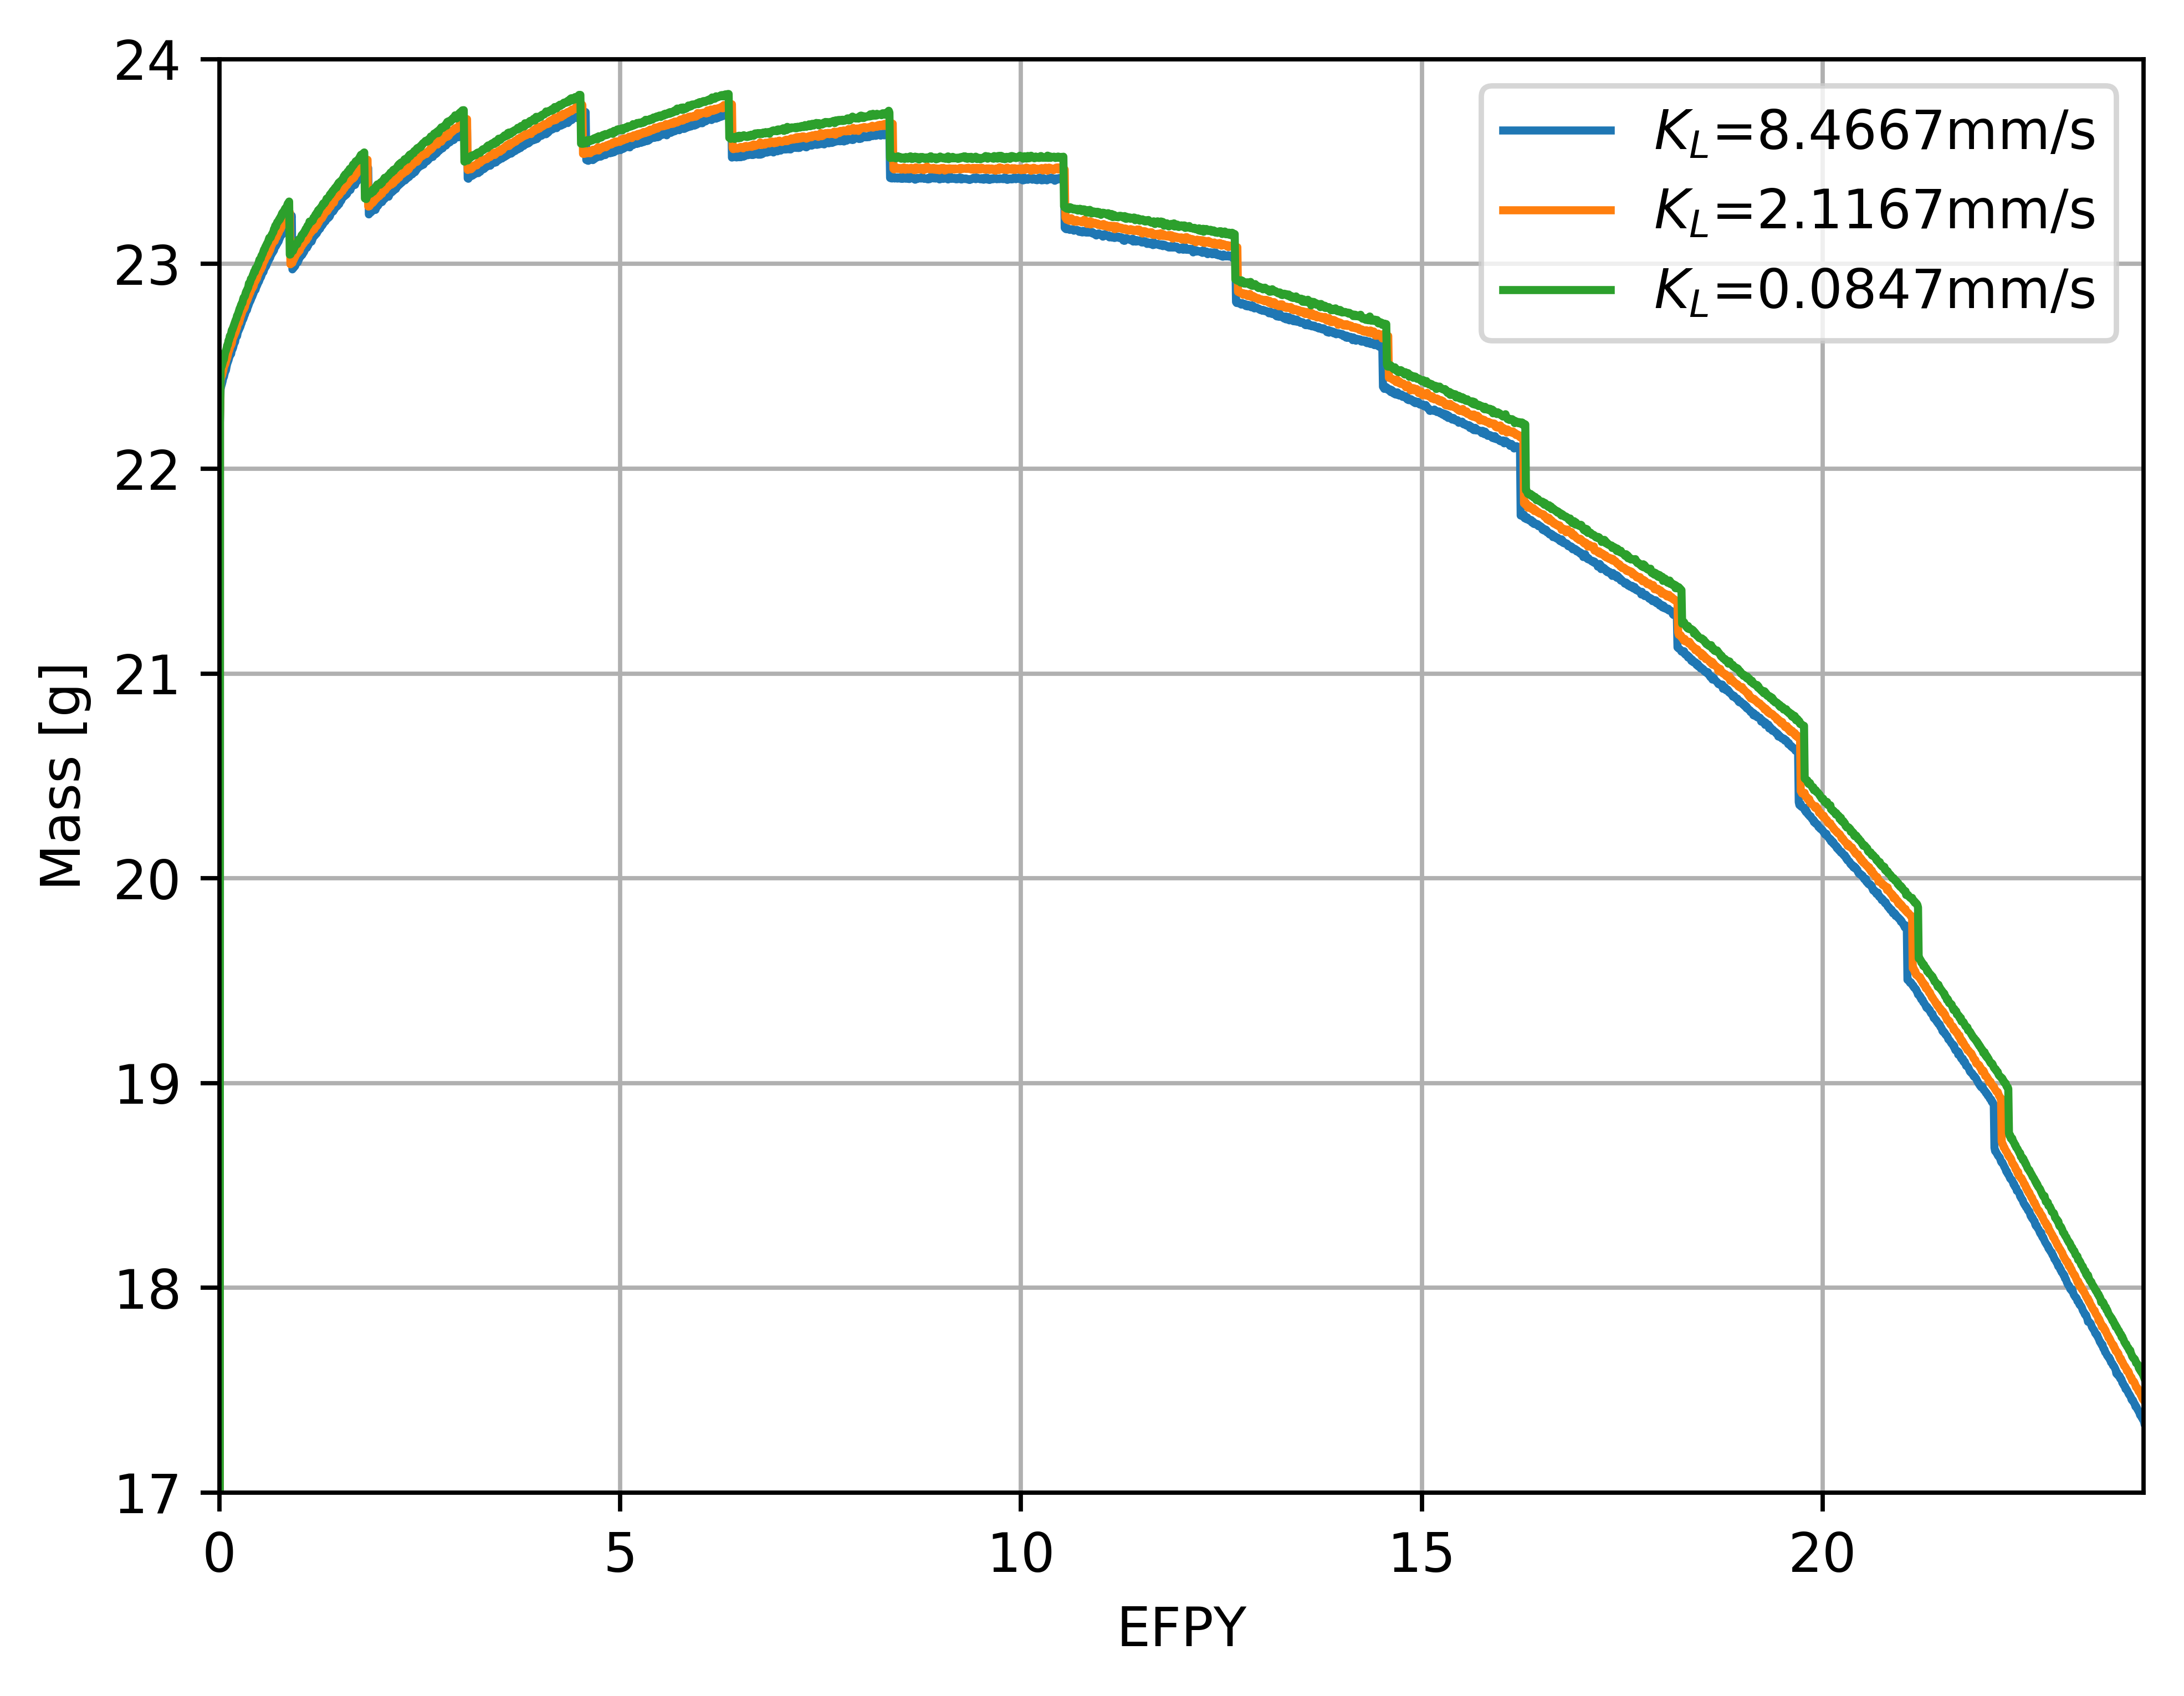
\includegraphics[width=0.85\textwidth]{ch4/eps/xe135.png}
	\caption{SaltProc-calculated mass of $^{135}$Xe in the fuel salt during 
		25 years of operation for the case with a realistic removal efficiency 
		of fission product and various mass transfer coefficients ($K_L$).}
	\label{fig:xe135-eps-var}
\end{figure}

I also performed an analytic verification to confirm SaltProc v1.0 correctness 
by comparing the mass of $^{135}$Xe to the expected mass after performing 
removals after each depletion step with realistic efficiency 
(Table~\ref{tab:gas_removal_efficiency}). The expected mass of a reprocessed 
isotope is calculated as follows:
\begin{align}
\qquad\qquad\qquad & m_{a} = m_{b} \times  
(1-\epsilon_{m}) \times (1-\epsilon_{es})
\intertext{where}
m_{a} &= \mbox{mass of the isotope after applying removals and feeds $[g]$} 
\nonumber \\
m_{b} &= \mbox{mass of the isotope right before reprocessing $[g]$} 
\nonumber \\
\epsilon_{m} &= \mbox{efficiency of the isotope migration to helium bubbles 
$[-]$} 
\nonumber \\
\epsilon_{es} &= \mbox{entrainment separator extraction efficiency $[-]$.} 
\nonumber
\end{align}

This simple check showed that the SaltProc-calculated mass of $^{135}$Xe 
(Figure~\ref{fig:xe135-eps-var-zoomes}) matches the expected mass exactly. 
Thus, SaltProc v1.0 extraction module correctly removes target isotopes with a
specified extraction efficiency. Finally, I added this correctness check as  
SaltProc v1.0 unit test.
\begin{figure}[htp!] % replace 't' with 'b' to 
	\centering
	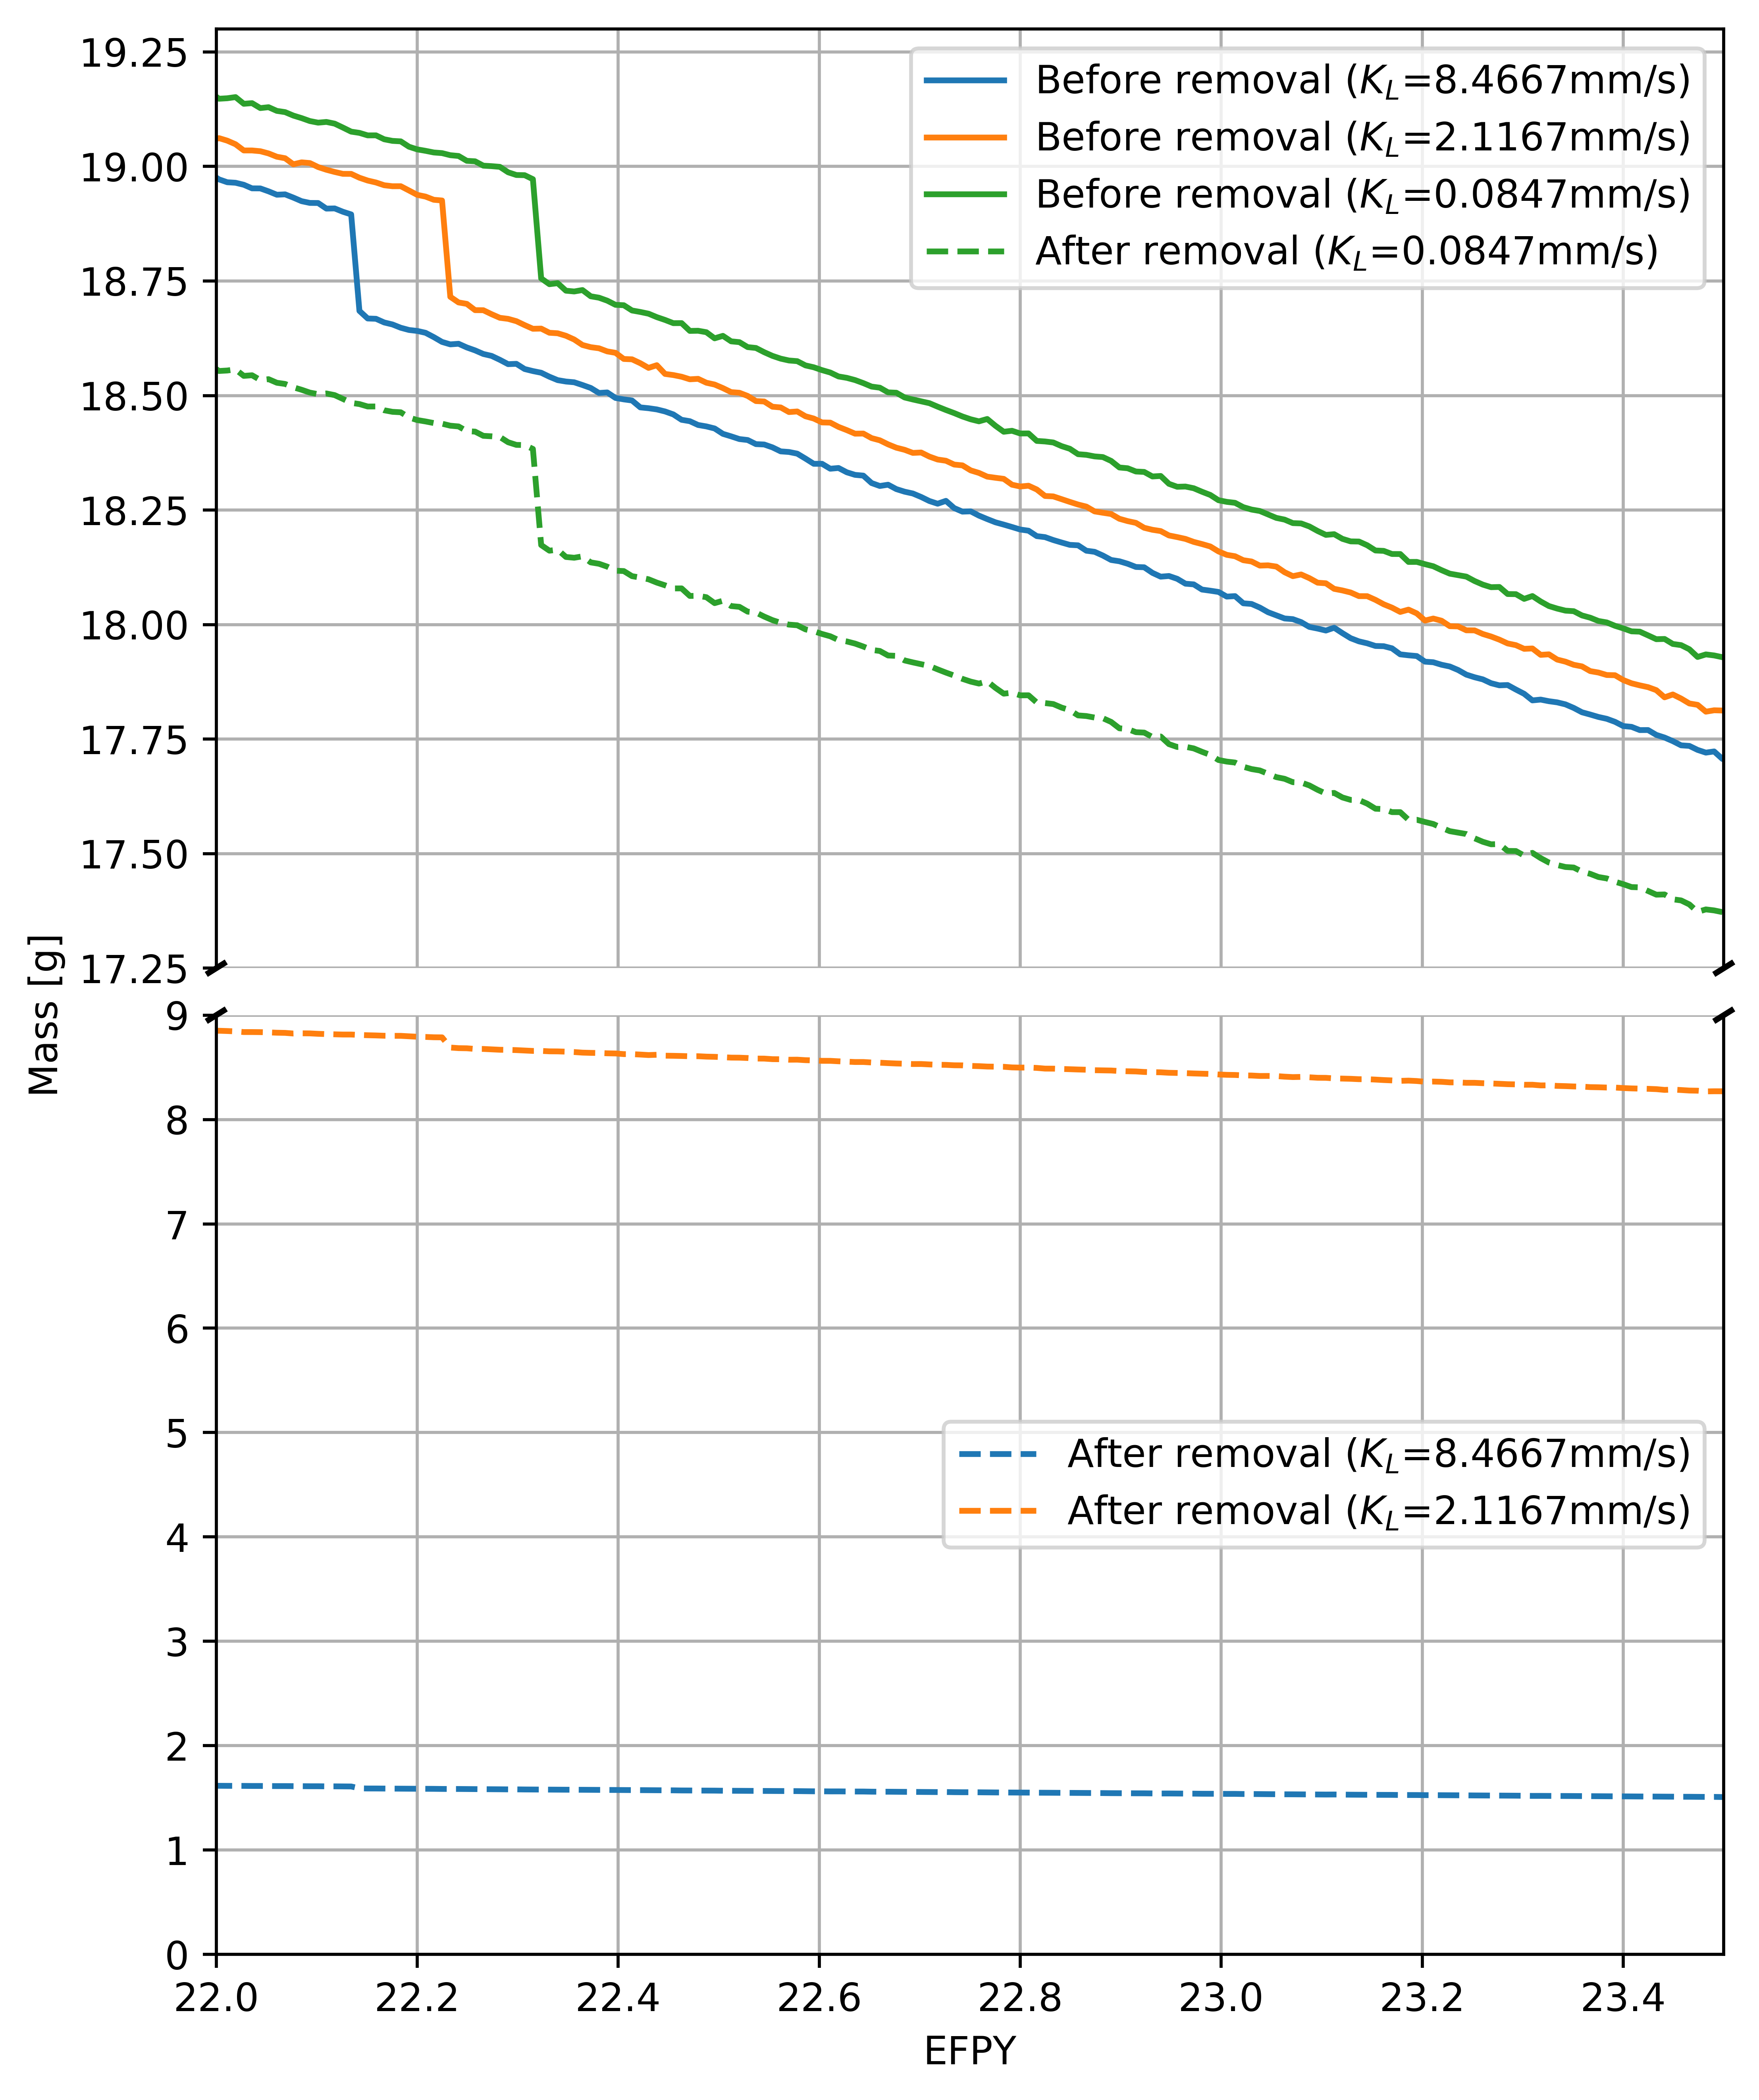
\includegraphics[width=\textwidth]{ch4/eps/xe135_zoomed_3.png}
	\caption{SaltProc-calculated mass of $^{135}$Xe in the fuel salt during 
	the last 18 months of operation for various mass transfer coefficients 
	($K_L$) at the end of each depletion step before and after performing the 
	salt treatment.}
	\label{fig:xe135-eps-var-zoomes}
\end{figure}
\FloatBarrier


\section{Safety and operational parameters} \label{sec:safety-param}
The previous section (Section~\ref{sec:long-term}) reported fuel salt 
composition evolution during 25 years of \gls{TAP} \gls{MSR} operation.
The inventory of fissile $^{235}$U decreased with time, while the inventories 
of fissile, $^{239}$Pu and $^{241}$Pu, increased. At 
the same time, many poisonous actinides (e.g., $^{236}$U, $^{240}$Pu, 
$^{242}$Pu) built up in the core, shifting the neutron energy 
spectrum. Moreover, the \gls{TAP} design assumes an intentional spectrum shift 
by adding more moderator rods during operation. In this section, I analyze how 
such neutron spectrum shift affects major safety and operational parameters 
such as temperature and void coefficients of reactivity, total control rod 
worth, and other reactor kinetic parameters.

\subsection{Temperature coefficient of reactivity}
The main physical principle underlying reactor temperature feedback is an 
expansion of heated material. When the fuel salt temperature increases, the 
density of the salt decreases, but at the same time, the total volume of fuel 
salt in the core remains constant because it is bounded by the vessel. When 
the moderator rod temperature increases, the density of zirconium hydride 
decreases, reducing space between moderator rods and displacing fuel salt from 
the core. Another physical principle underlying temperature feedback is the 
Doppler broadening of the resonance capture cross section of the $^{238}$U 
due to thermal motion of target nuclei in the fuel. The Doppler effect 
arises from the dependence of the capture cross sections on the relative 
velocity between neutron and nucleus. The Doppler coefficient of reactivity of 
thermal reactors is always negative and instantaneous.

The temperature coefficient of reactivity, $\alpha$, quantifies reactivity 
changes due to temperature change in fuel and moderator component of a reactor 
core. The $\alpha_{T,j}$ represents the temperature coefficient of 
reactivity of a component $j$ (fuel, moderator, or isothermal) and can be 
calculated as:
\begin{align}\label{eq:th-feedback}
\alpha_{T,j} &= \frac{\partial \rho}{\partial T_j} \quad[pcm/K]
\intertext{where}
\rho       &= \frac{k_{eff}-1}{k_{eff}} \times 10^5 \quad[pcm] \\
k_{eff}  &= \mbox{effective multiplication factor corresponding to $T$ of 
component $j$ [$-$]} \nonumber \\
\partial T_j &= \mbox{change in average temperature of component $j$ 
[$K$]}.\nonumber
\end{align}
If the temperature change is assumed to be uniform throughout the core, the 
temperature coefficient of reactivity is usually called Total or Isothermal 
Temperature Coefficient (ITC), $\alpha_{T,ISO}$, and can be defined as the 
change in reactivity per unit of temperature change:
\begin{align}\label{eq:itc-feedback}
\alpha_{T,ISO} &= \frac{\Delta\rho}{\Delta T} \quad[pcm/K] \\
\intertext{where}
\Delta\rho  &= \mbox{change in reactivity [$pcm$]} \nonumber \\
\Delta T_j &= \mbox{change in average temperature of the core [$K$]}.\nonumber
\end{align}

However, fuel and moderator temperature are rarely equal because fuel heats up 
much faster than the moderator; thus, the fuel temperature coefficient 
($\alpha_{T,F}$ or FTC) and the moderator temperature coefficient 
($\alpha_{T,M}$ or MTC) must be calculated 
separately. In the base case simulation in this work, the fuel salt and the 
moderator temperatures are fixed at 900K. To determine $\alpha_{T,F}$, I 
perturbed the fuel salt temperature from 800K to 1000K in 
increments of 50K while fixing the moderator temperature at 900K (base case). 
Likewise, I calculated $\alpha_{T,M}$ by perturbing the moderator temperature 
from 800K to 1000K with 50K increments, while fixing the fuel temperature at 
900K. 

The range of temperature perturbation for the temperature coefficient  
calculation has been selected based on operational parameters. The \gls{TAP} 
\gls{MSR} operates in the range of 773-973K (500-700$^{\circ}$C), which is far 
below the salt boiling point of approximately 1473K 
\cite{transatomic_power_corporation_technical_2016}. The salt freezes below 
773K \cite{barton_phase_1958}. At the other end of the temperature spectrum, 
the temperature higher than 973K passively melts a freeze plug, which drains 
the fuel salt from the reactor vessel to the drain tanks. The drain tanks have 
a subcritical configuration with a large free surface area to readily 
dissipate heat by passive cooling 
\cite{transatomic_power_corporation_technical_2016}. 
Thus, calculating temperature coefficients in the temperature range from 800 
to 1000K captured the outcomes of most accident transients.

To determine the temperature coefficients, the cross section temperatures for 
the fuel and moderator were changed in the range of 800-1000K. For 
$\alpha_{T,F}$ calculation, changes in the fuel temperature impact cross 
section resonances (Doppler effect) as well as the fuel salt density. The 
density of fuel salt changes with respect to temperature as follows 
\cite{janz_molten_1974}:
\begin{align}\label{eq:salt-den}
\rho_{salt}(T) &= 6.105 - 12.720\times10^4 T[K] \quad [g/cm^3]
\end{align}
The uncertainty in the salt density calculated using 
Equation~\ref{eq:salt-den} is approximately 0.036 $g/cm^3$ at 900K.
In contrast, when the moderator temperature changes, the density, cross 
section temperature, and the geometry also change due to thermal 
expansion of the solid zirconium hydride (ZrH$_{1.66}$) rods. Accordingly, the 
new moderator density and sizes are calculated using a linear temperature 
expansion coefficient \cite{yamanaka_thermal_1999}:
\begin{align}
\alpha_L &= 2.734\times10^{-5} \quad [K^{-1}]
\end{align}
Using this thermal expansion data, I took into account the displacement of the 
moderator surfaces by generating corresponding geometry definitions for each 
Serpent calculation. That is, $\alpha_{T,M}$ calculation takes into account 
the following factors:
\begin{itemize}[noitemsep, topsep=0pt]
	\item thermal Doppler broadening of the resonance capture cross sections 
	in ZrH$_{1.66}$;
	\item hydrogen S($\alpha$, $\beta$) thermal scattering data shift due to 
	moderator temperature change;
	\item density change due to moderator thermal expansion/contraction;
	\item corresponding geometric changes in the moderator rod diameter and 
	length.
\end{itemize}
 
By propagating the $k_{eff}$ statistical error provided by Serpent 2, the 
corresponding uncertainty in each temperature coefficient is obtained using 
the formula:
\begin{align}
\delta\alpha_T &= \abs{\frac{1}{T_{i+1} - T_i}} \sqrt{\frac{\delta 
		k_{eff}^2(T_{i+1})}{k_{eff}^4(T_{i+1})}  
	+ \frac{\delta k_{eff}^2(T_i)}{k_{eff}^4(T_i)}}
\intertext{where}
k_{eff} &= \mbox{effective multiplication factor corresponding to $T_i$ [-]} 
\nonumber \\
\delta k_{eff} &= \mbox{statistical error for $k_{eff}$ from Serpent output 
[$pcm$]} \nonumber \\
T_i &= \mbox{perturbed temperature in the range of 800-1000K.} \nonumber
\end{align}
Notably, other sources of uncertainty are neglected, such as design parameter 
uncertainty, cross section measurement error\footnote{Chapter 7 of the current 
work presents uncertainty quantification method for propagating cross section 
measurement uncertainty throughout depletion calculations. While it is out of 
scope of this work to estimate nuclear-data related uncertainty of the 
temperature feedback coefficient, method from Chapter 7 can be adopted for the 
future work to perform such calculations.}, and approximations inherent in 
the equations of state providing both the salt and moderator density 
dependence on temperature. 

Figure~\ref{fig:tc-bol-eol} shows reactivity as a function of fuel, moderator, 
and total temperature for the \gls{TAP} \gls{MSR} at the \gls{BOL} and 
\gls{EOL}. At startup, reactivity change with temperature clearly fits 
linear regression (R-squared\footnote{Coefficient of determination ($R^2$) is 
a statistical measure of how good measured data fitted linear regression 
line.} is 0.9, 0.99, and 0.98 for fuel, moderator, and isothermal case, 
respectively). 
Also, while the linear relationship between reactivity and moderator 
temperature worsens toward the \gls{EOL}, an $R^2>0.7$ still indicates a 
strong linear association between $\rho$ and $T$ ($R^2$ is 0.99, 0.87, and 
0.74 for fuel, 
moderator, and total case, respectively). I determined the temperature 
coefficient of reactivity separately for each component (fuel, moderator, 
and isothermal) using the slope of the linear regression for each.

\begin{figure}[htbp!] % replace 't' with 'b' to 
	\centering
	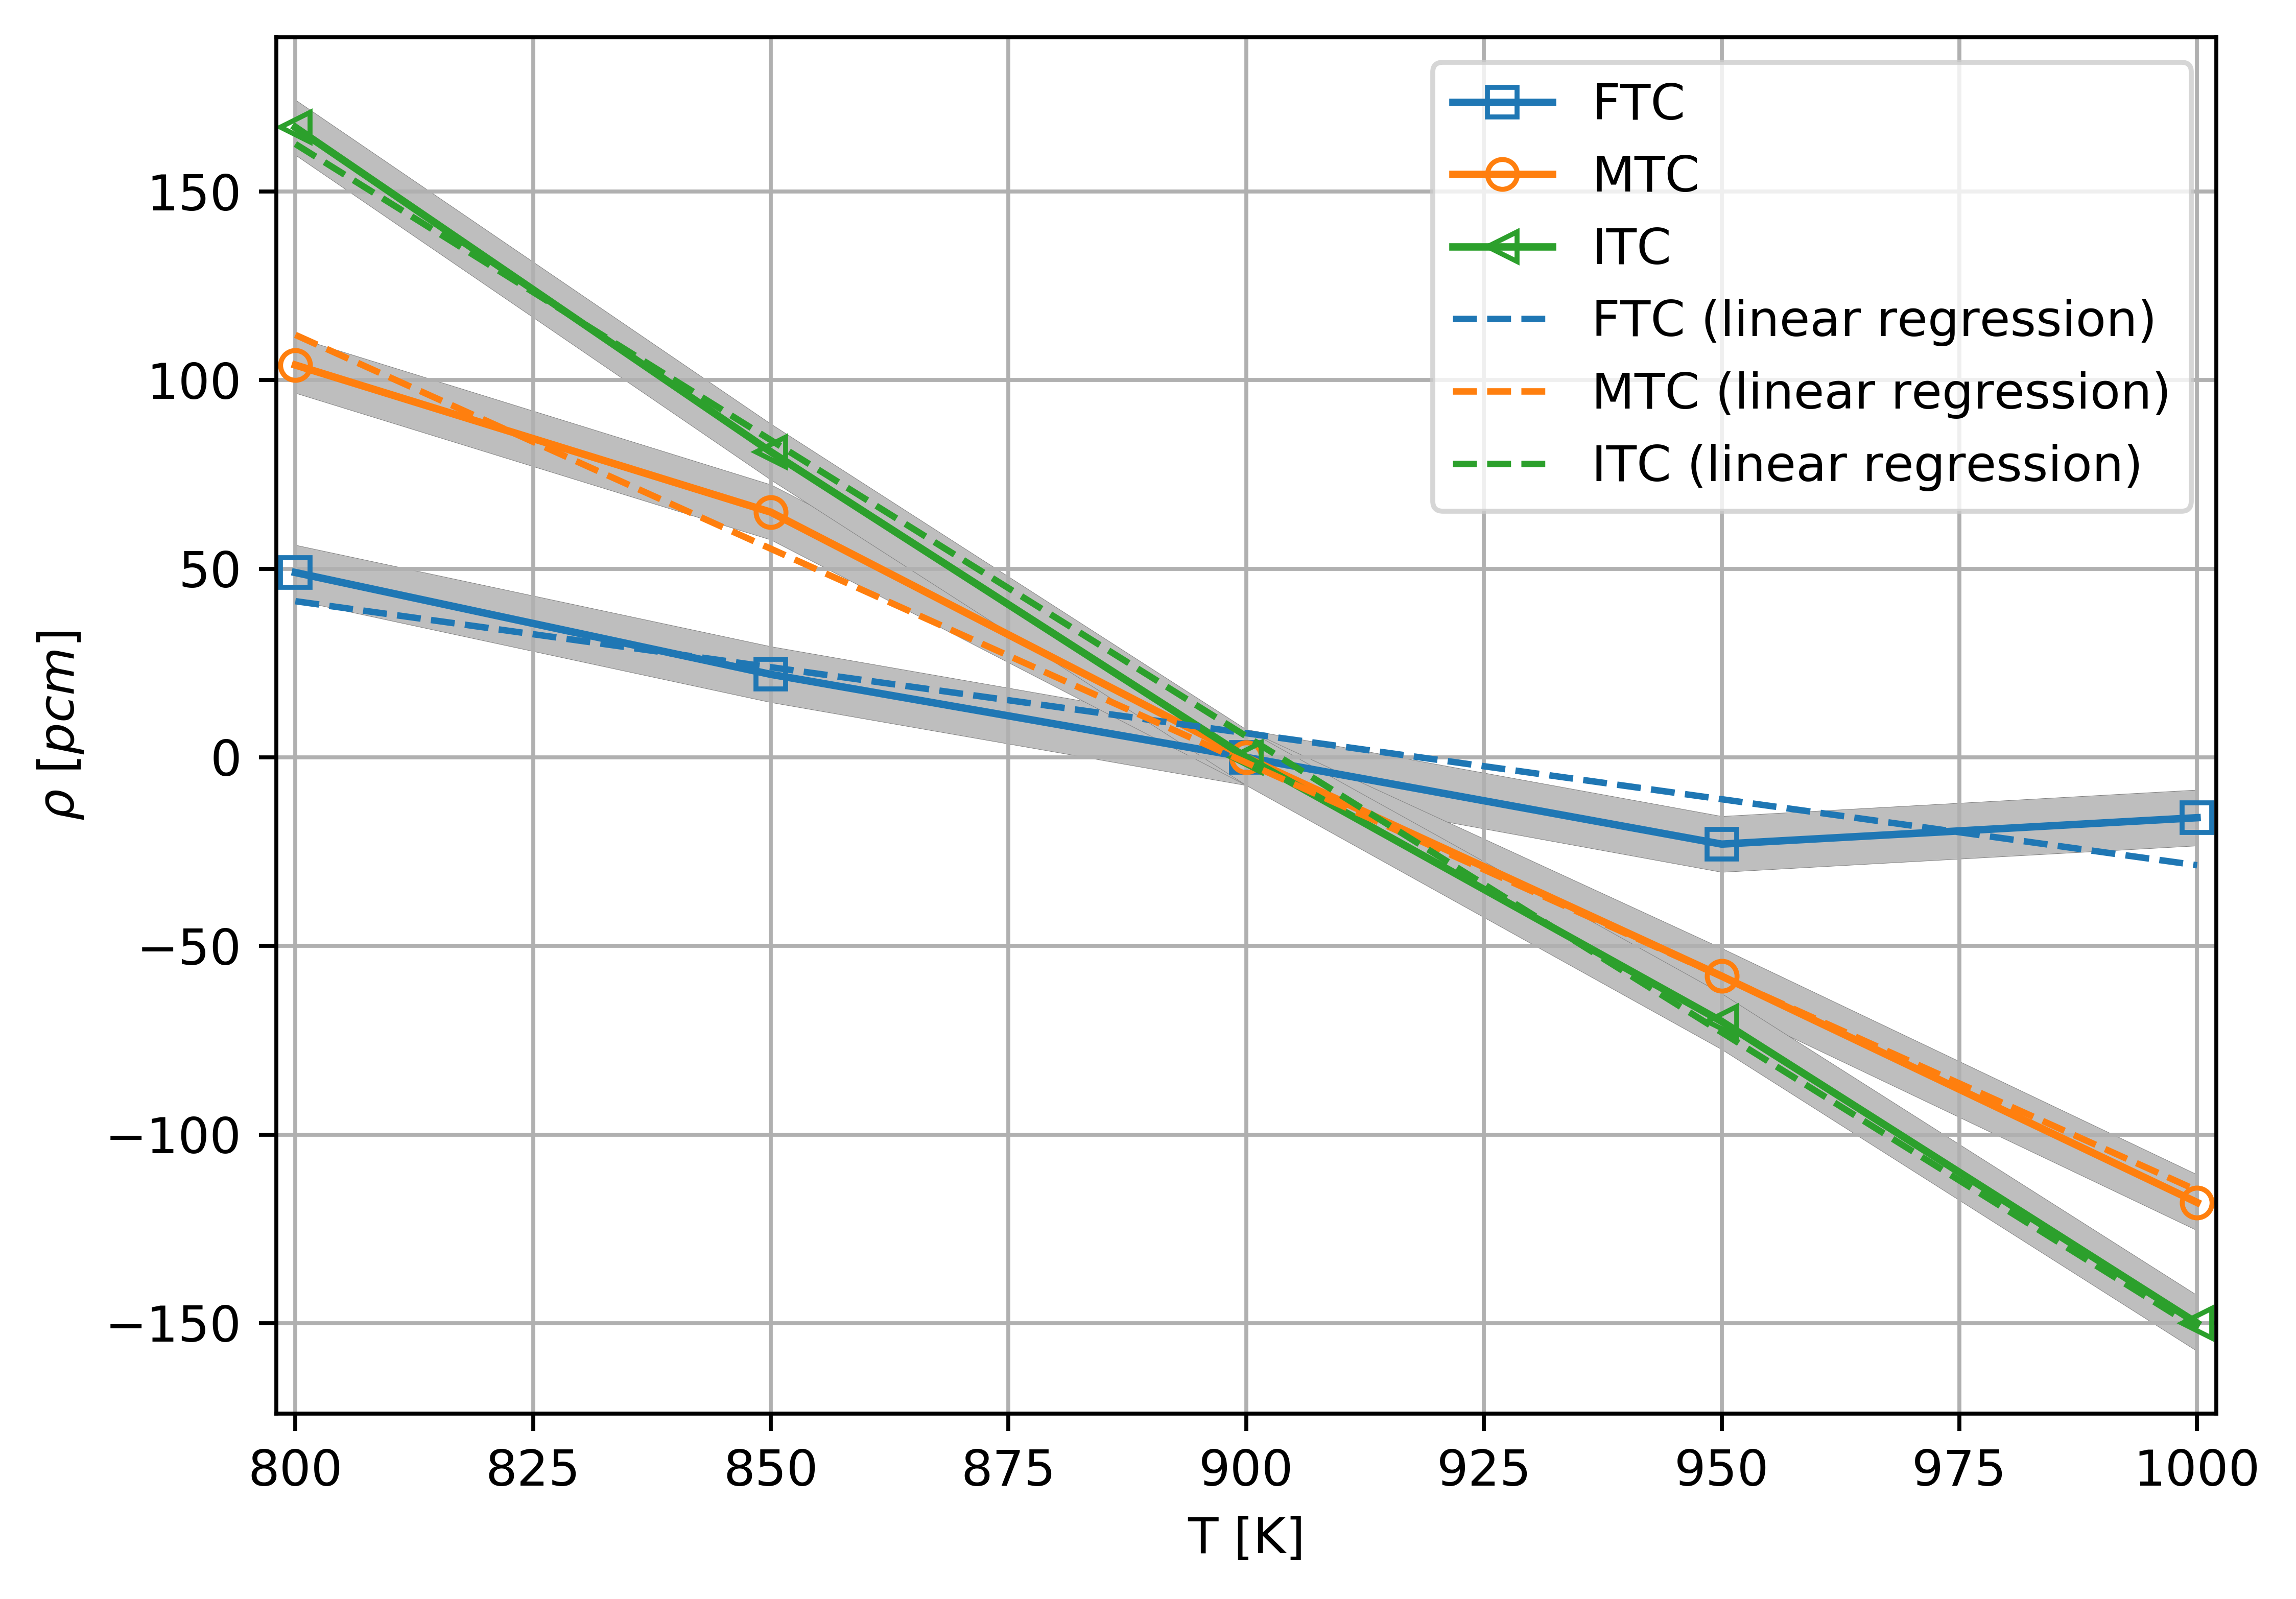
\includegraphics[width=0.97\textwidth]{ch4/saf_par/tc_bol.png}\\
	\vspace{-12mm}
	\hspace{+0.05mm}
	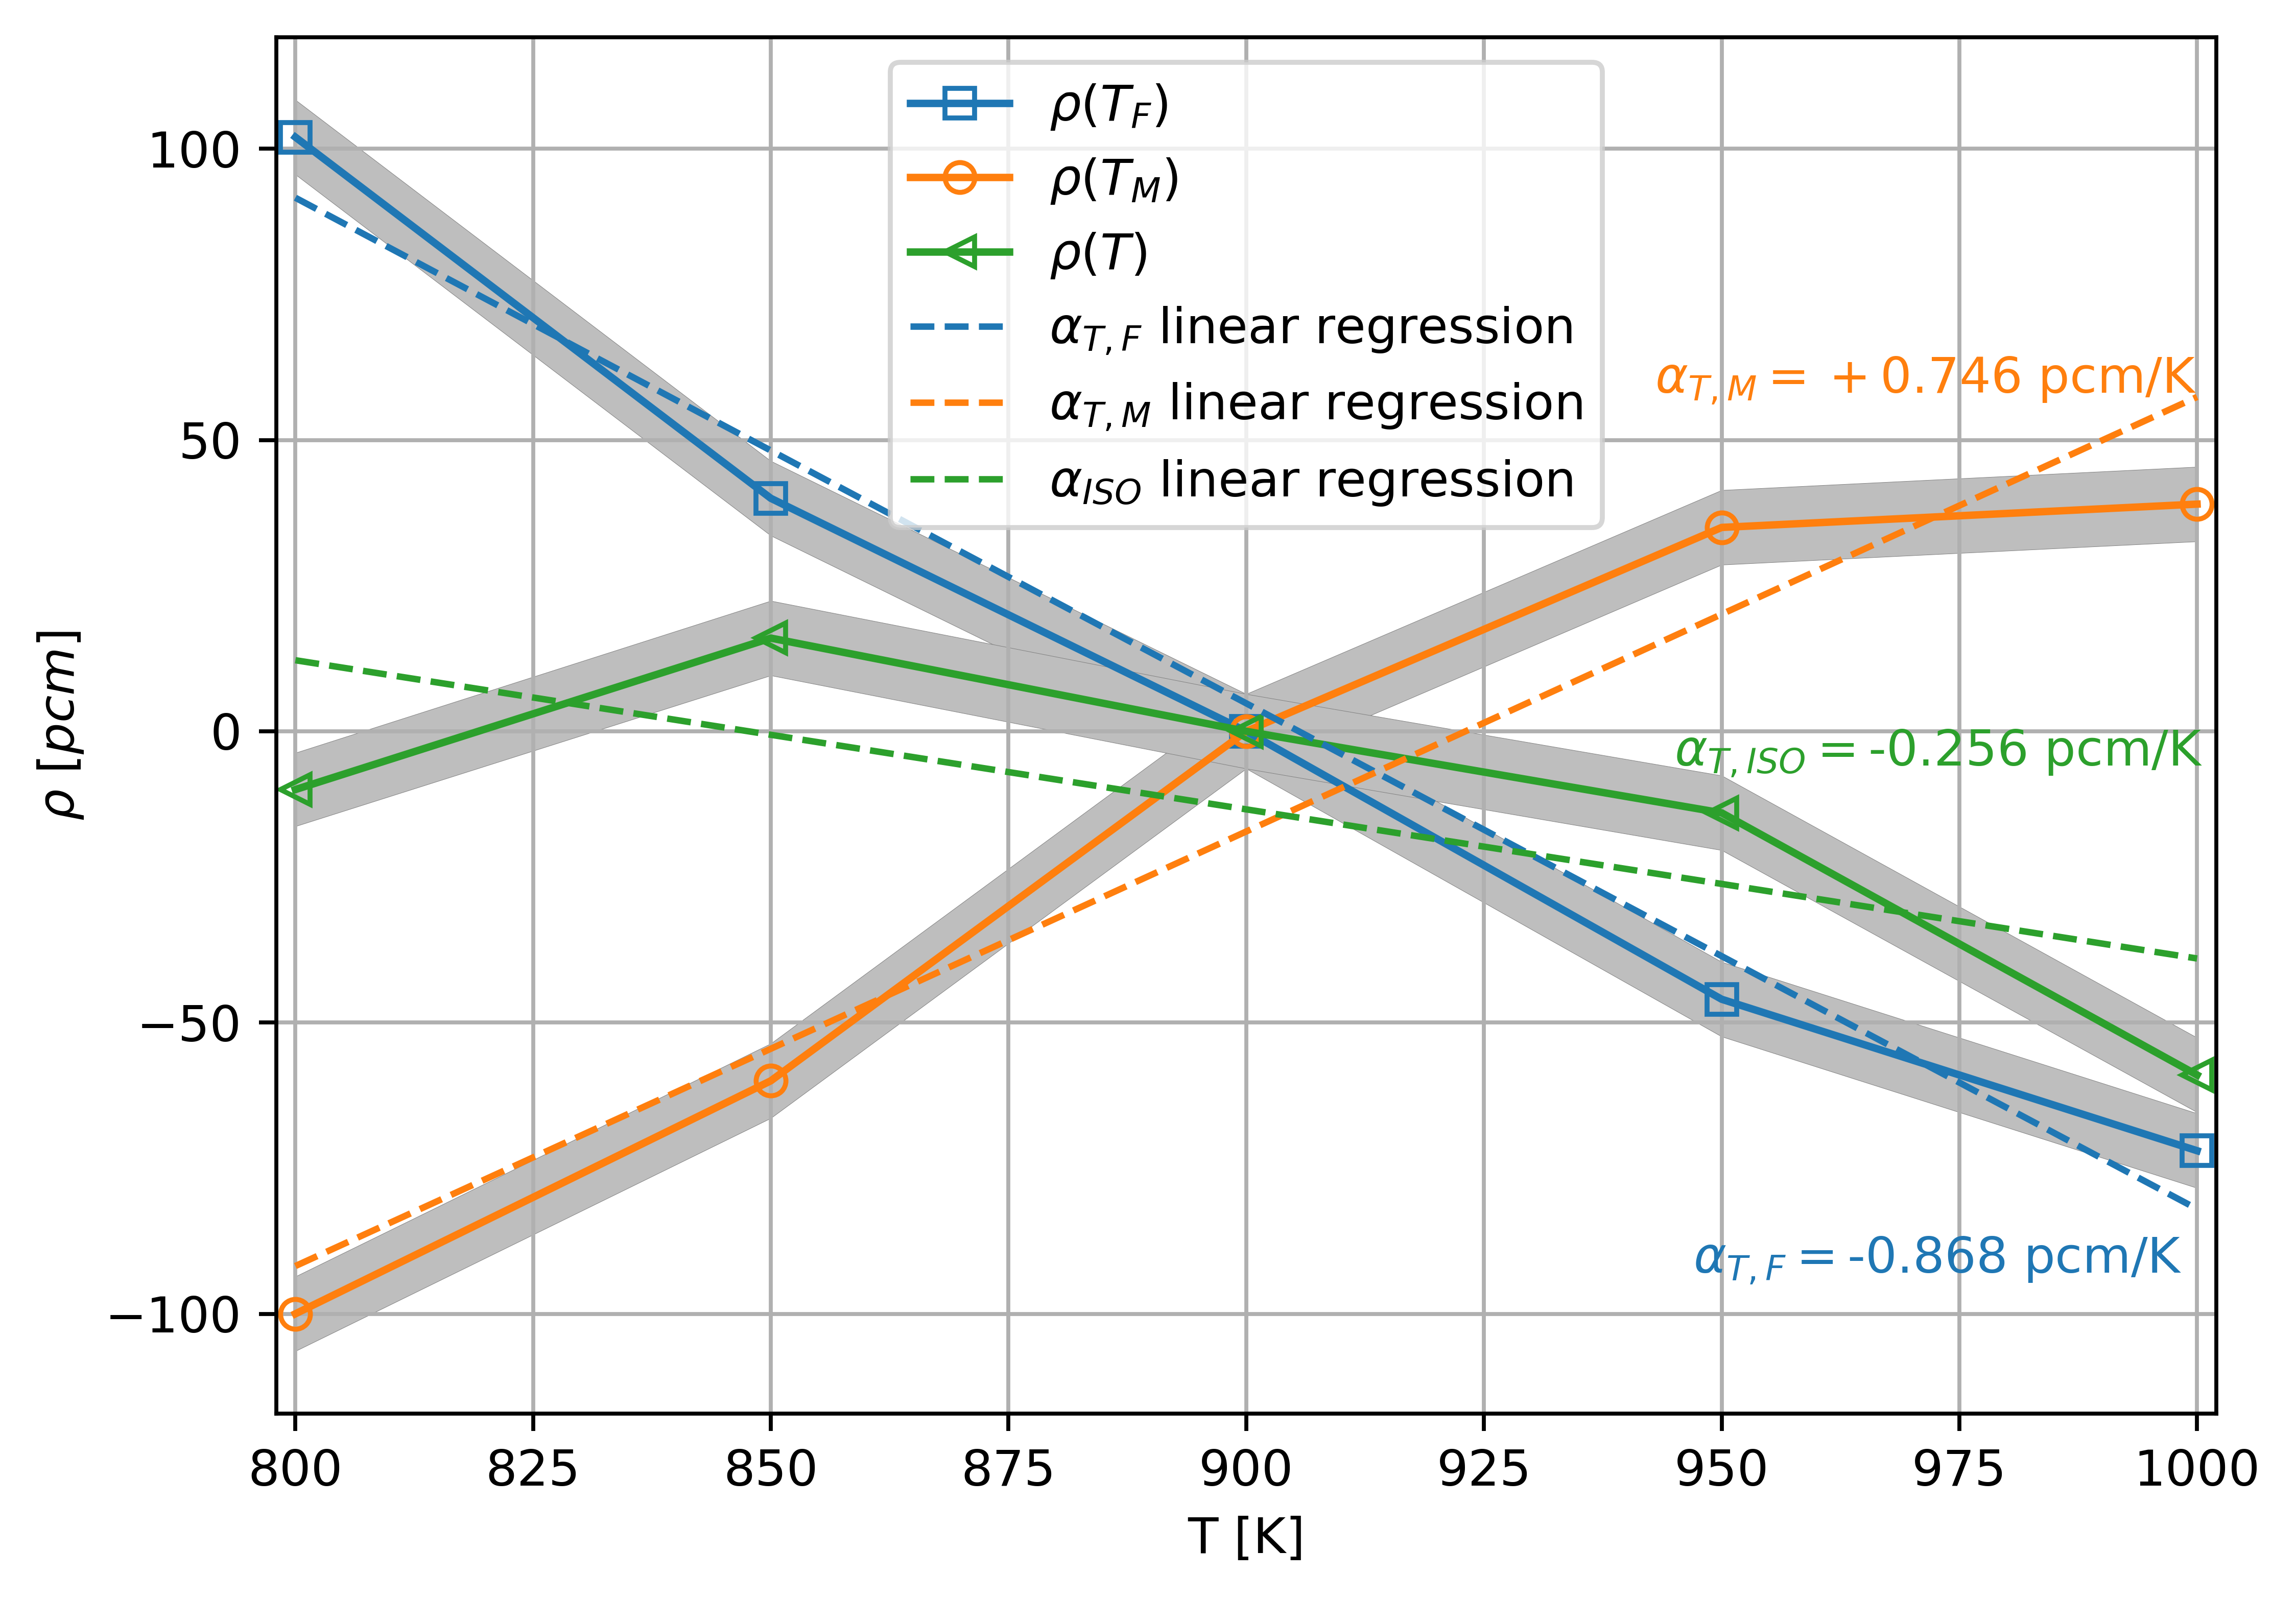
\includegraphics[width=0.97\textwidth]{ch4/saf_par/tc_eol.png}
	\vspace{-3mm}
	\caption{Serpent-calculated reactivity as a function of fuel salt 
		(blue), moderator (orange), and both fuel/moderator (green) 
		temperature 
		at 	\gls{BOL} (upper) and \gls{EOL} (lower). The uncertainty 
		$\pm\sigma$ region is shaded.}
	\label{fig:tc-bol-eol}
\end{figure}

Table~\ref{tab:tcoef_tap} summarizes temperature coefficients of reactivity in 
the 
\gls{TAP} core calculated at the \gls{BOL} and \gls{EOL}. The fuel 
temperature coefficient is negative throughout operation and becomes stronger 
toward the \gls{EOL} as the spectrum thermalizes due to additional, retained 
fission products and actinides building up in the fuel salt. 
The MTC and ITC are both strongly negative at startup. However, the MTC became 
weakly positive toward the \gls{EOL} due to the same spectral shift. To better 
understand the dynamics of temperature coefficient evolution, I calculated 
temperature coefficients for 15 distinct moments during operation to cover all 
moderator rod configurations described in Appendix~A.
%%%%%%%%%%%%%%%%%%%%%%%%%%%%%%%%%%%%%%%%
\begin{table}[ht!]
	\caption{Temperature coefficients for the \gls{TAP} reactor at the 
	\gls{BOL} and \gls{EOL}.}
		\centering
	\begin{tabularx}{0.6\textwidth}{ X  r r } \hline
		\textbf{Coefficient} & \textbf{\gls{BOL} [pcm/K]} & \textbf{\gls{EOL} 
		[pcm/K]}                  \tabularnewline 
		[5pt] \hline
		FTC & $-0.350\pm0.050$ & $-0.868\pm0.045$ 
		\tabularnewline [3pt] \hline
		MTC & $-1.134\pm0.050$ & $+0.746\pm0.045$  
		\tabularnewline [3pt] \hline
		ITC & $-1.570\pm0.050$ & $-0.256\pm0.045$  
		\tabularnewline [3pt] \hline
	\end{tabularx}
	\label{tab:tcoef_tap}
\end{table}
%%%%%%%%%%%%%%%%%%%%%%%%%%%%%%%%%%%%%%%%%%%%%%%%%%%%%%%%%%%%%%%%%%%%%%%%%%%%%%%%

Figure~\ref{fig:tc-evo} shows temperature coefficient evolution for the 
\gls{TAP} reactor during 25 years of operation and takes into account the
spectral shift due to moderator rod reconfigurations. The fuel temperature 
coefficient is almost 
constant for 19 years but decreases for the last 6 years (configurations with 
1498 and 1668 moderator rods in the core). In contrast, the moderator 
temperature coefficient decreases from $-1.134$ $pcm$/$K$ to $-2.280$ 
$pcm$/$K$ during the first 11 years and then increases up to $+0.746$ 
$pcm$/$K$ at the \gls{EOL}. 
The moderator temperature increase at startup pushes thermal neutrons to 
higher energies, nearly up to the lowest 
$^{238}$U resonances in the capture cross section. After 11 years, similar 
moderator temperature increase shifts neutrons into the same 
energy region, but this time that energy range is populated not only with 
$^{238}$U but also with low-lying resonances from the actinides and fission 
products.

Additionally, the moderator temperature coefficient increases after 11 years 
of operation because there is twice as much moderator in the core at 11 years 
compared to the \gls{BOL}. The moderator temperature increase causes fuel 
salt displacement due to the thermal expansion of the moderator rods, which 
has a particularly strong effect when the salt volume fraction is less than 
75\%. That is, when moderator heats up, the moderator-to-fuel ratio increases 
due to thermal expansion of zirconium hydride, which in turn leads to positive 
change in reactivity. %These 
%observations from estimating reactivity coefficients demonstrate the 
%importance of proper characterization of thermal scattering data for the 
%zirconium hydride moderator.

Finally, the isothermal temperature coefficient dynamics are similar to the 
MTC:
the ITC decreases from $-1.57$ $pcm/K$ to $-2.66$ $pcm/K$ first 13 years of 
operation. After that, the ITC grows rapidly up to $-0.256$ $pcm/K$ at the 
\gls{EOL}. Overall, the ITC remains negative throughout operation but became 
relatively weak after 25 years of operation (comparing with conventional 
\gls{PWR}, which has an isothermal temperature coefficient of 
$\alpha_{T,ISO}\approx-3.08$ $pcm/K$ \cite{forget_integral_2018}).
\begin{figure}[htp!] % replace 't' with 'b' to 
	\centering
	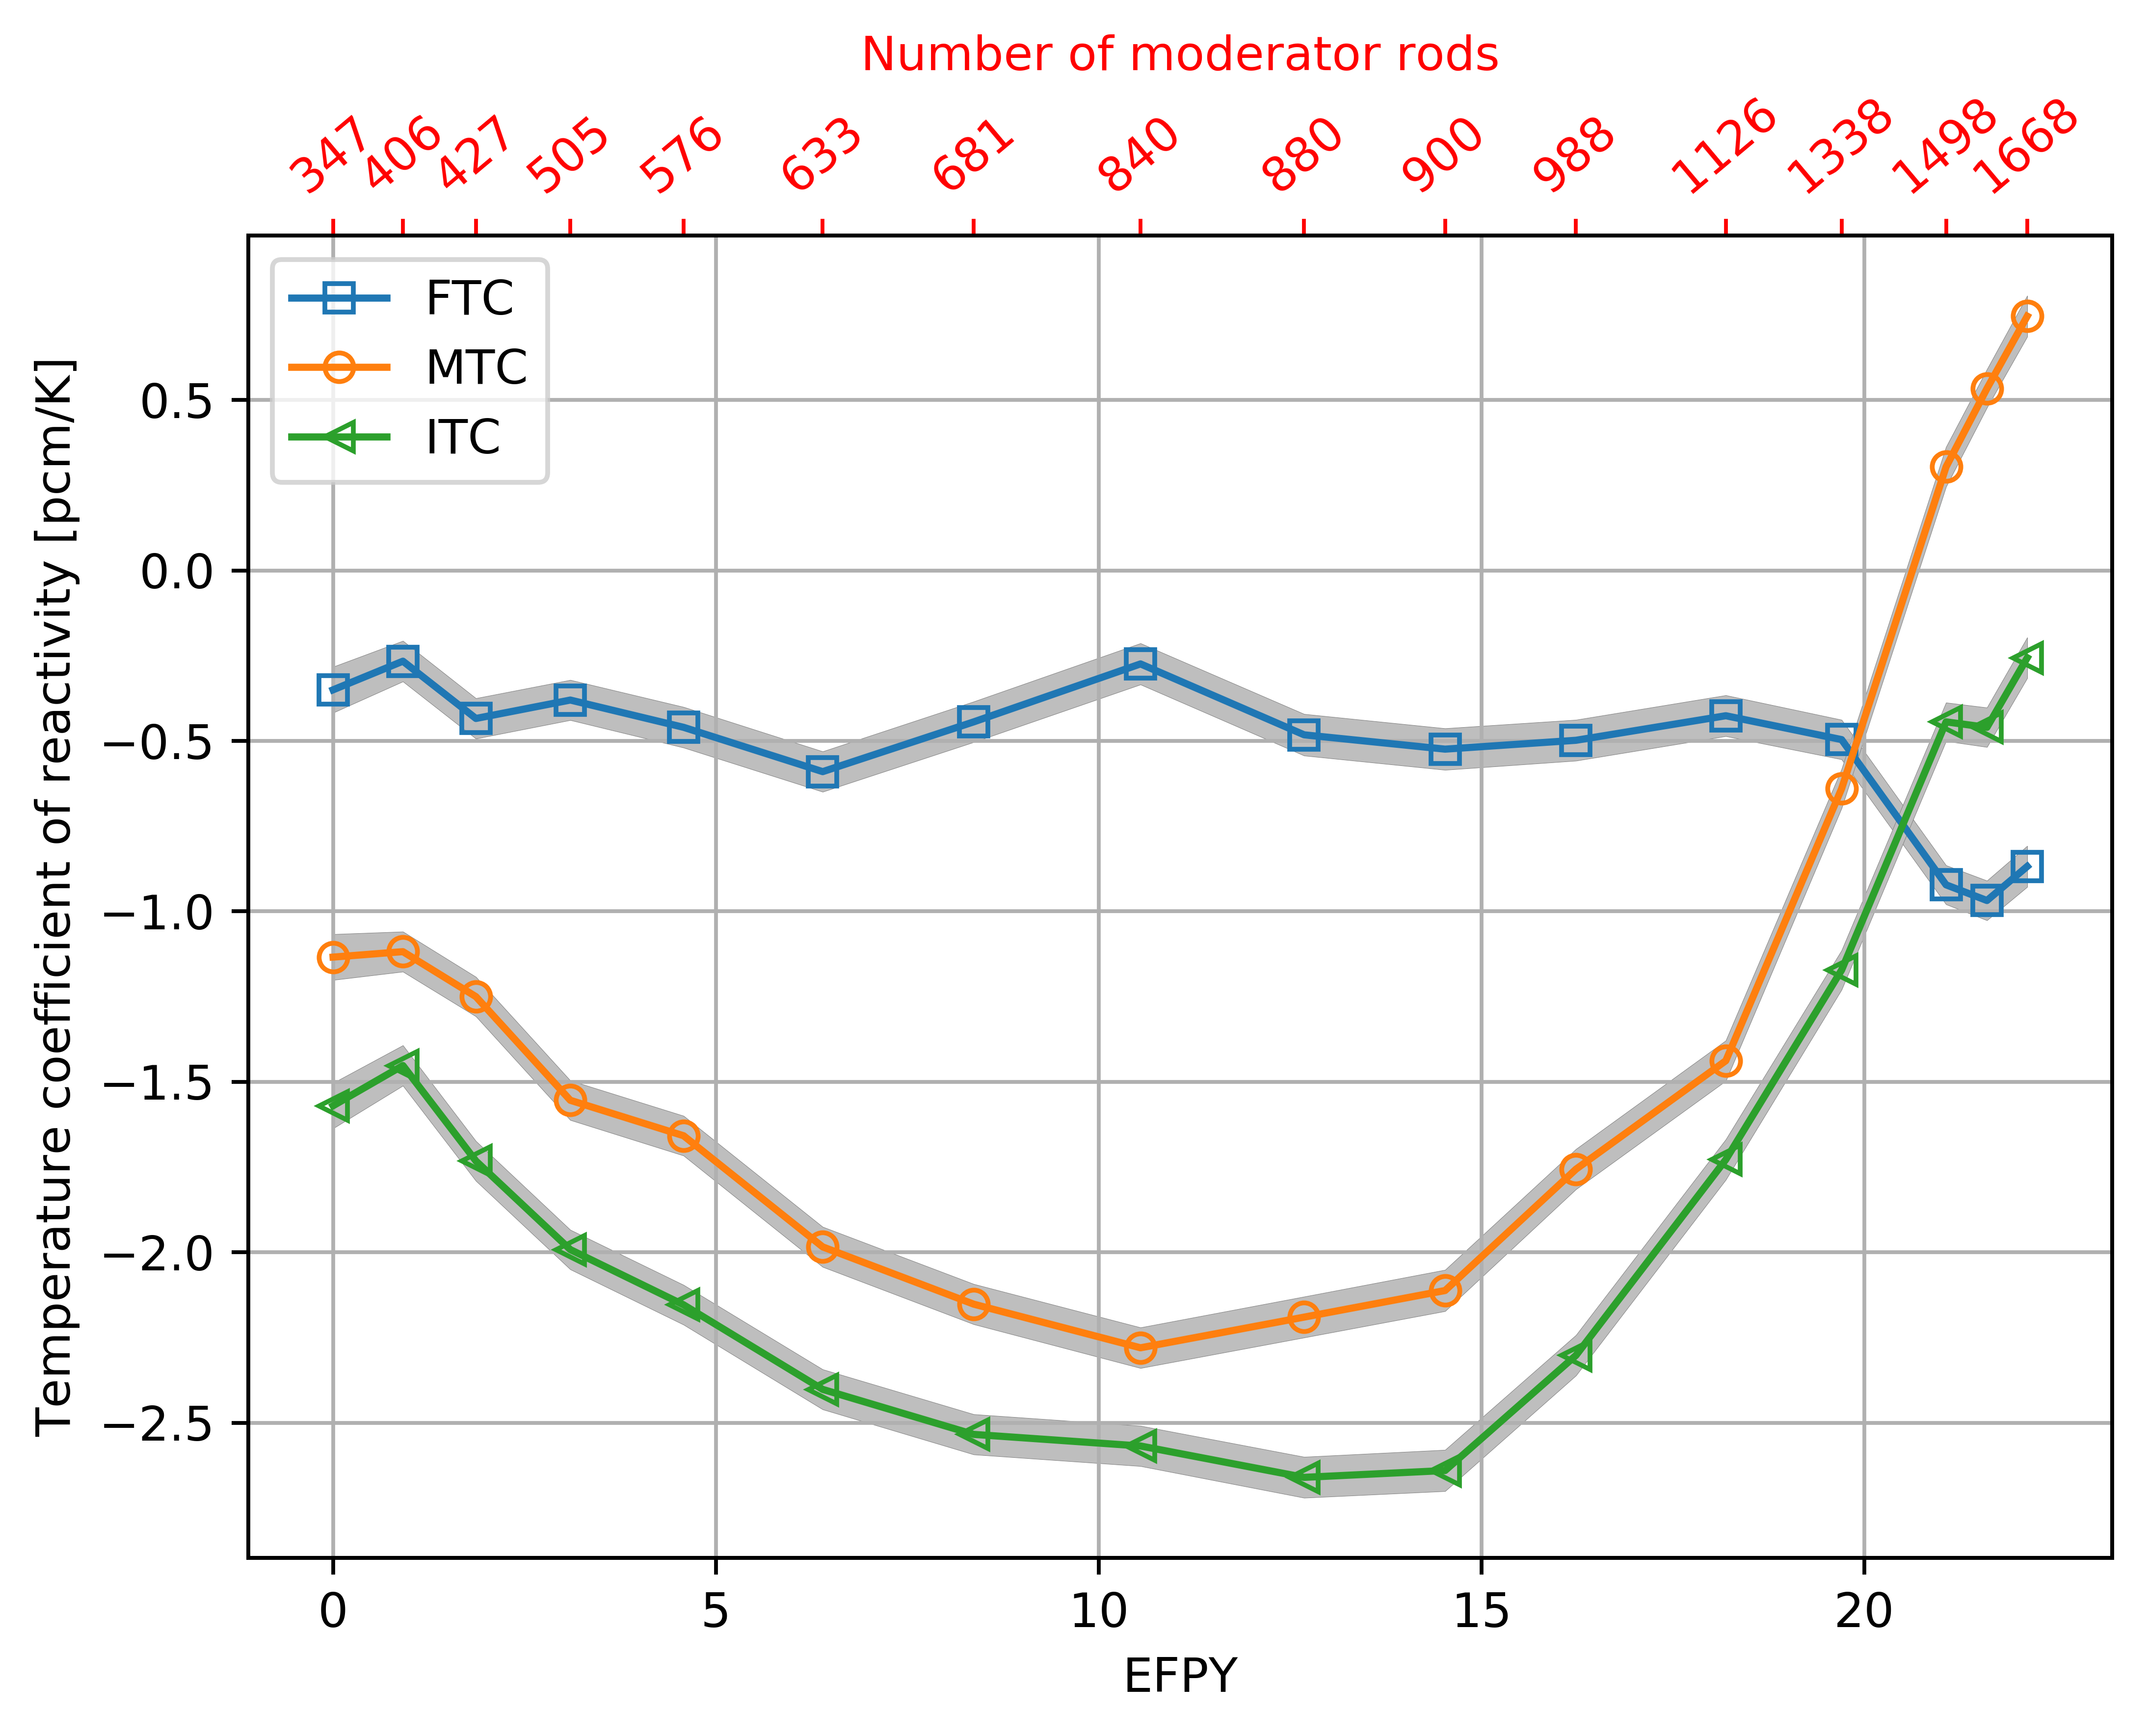
\includegraphics[width=\textwidth]{ch4/saf_par/tc_evo.png}
	\caption{Serpent-calculated fuel, moderator, and isothermal temperature 
		coefficients of reactivity as a function of time and number of 
		moderator 
		rods in the \gls{TAP} core. The uncertainty $\pm\sigma$ region is 
		shaded.}
	\label{fig:tc-evo}
\end{figure}

\subsection{Void coefficient of reactivity}
The effect of fuel voids (i.e. bubbles) on reactivity is evaluated by reducing 
the fuel salt density from the base value (0\% void) assuming helium volume 
fraction in the salt varies between 0 and 2\%. The temperatures of both the 
fuel salt and the moderator are held constant at 900K. 
Because a decrease in the salt density causes an increase of moderator-to-fuel 
ratio, an increase in the helium volume fraction (voids) increases reactivity 
as shown in Figure~\ref{fig:void-bol-eol}.
However, the slope of the line (void coefficient of reactivity ($\alpha_{V}$)) 
decreases toward \gls{EOL} due to the gradually increasing volume of moderator 
in the core (the volume fraction of the fuel salt at the \gls{EOL} is less 
than 54\%).
\begin{figure}[htp!] % replace 't' with 'b' to 
	\centering
	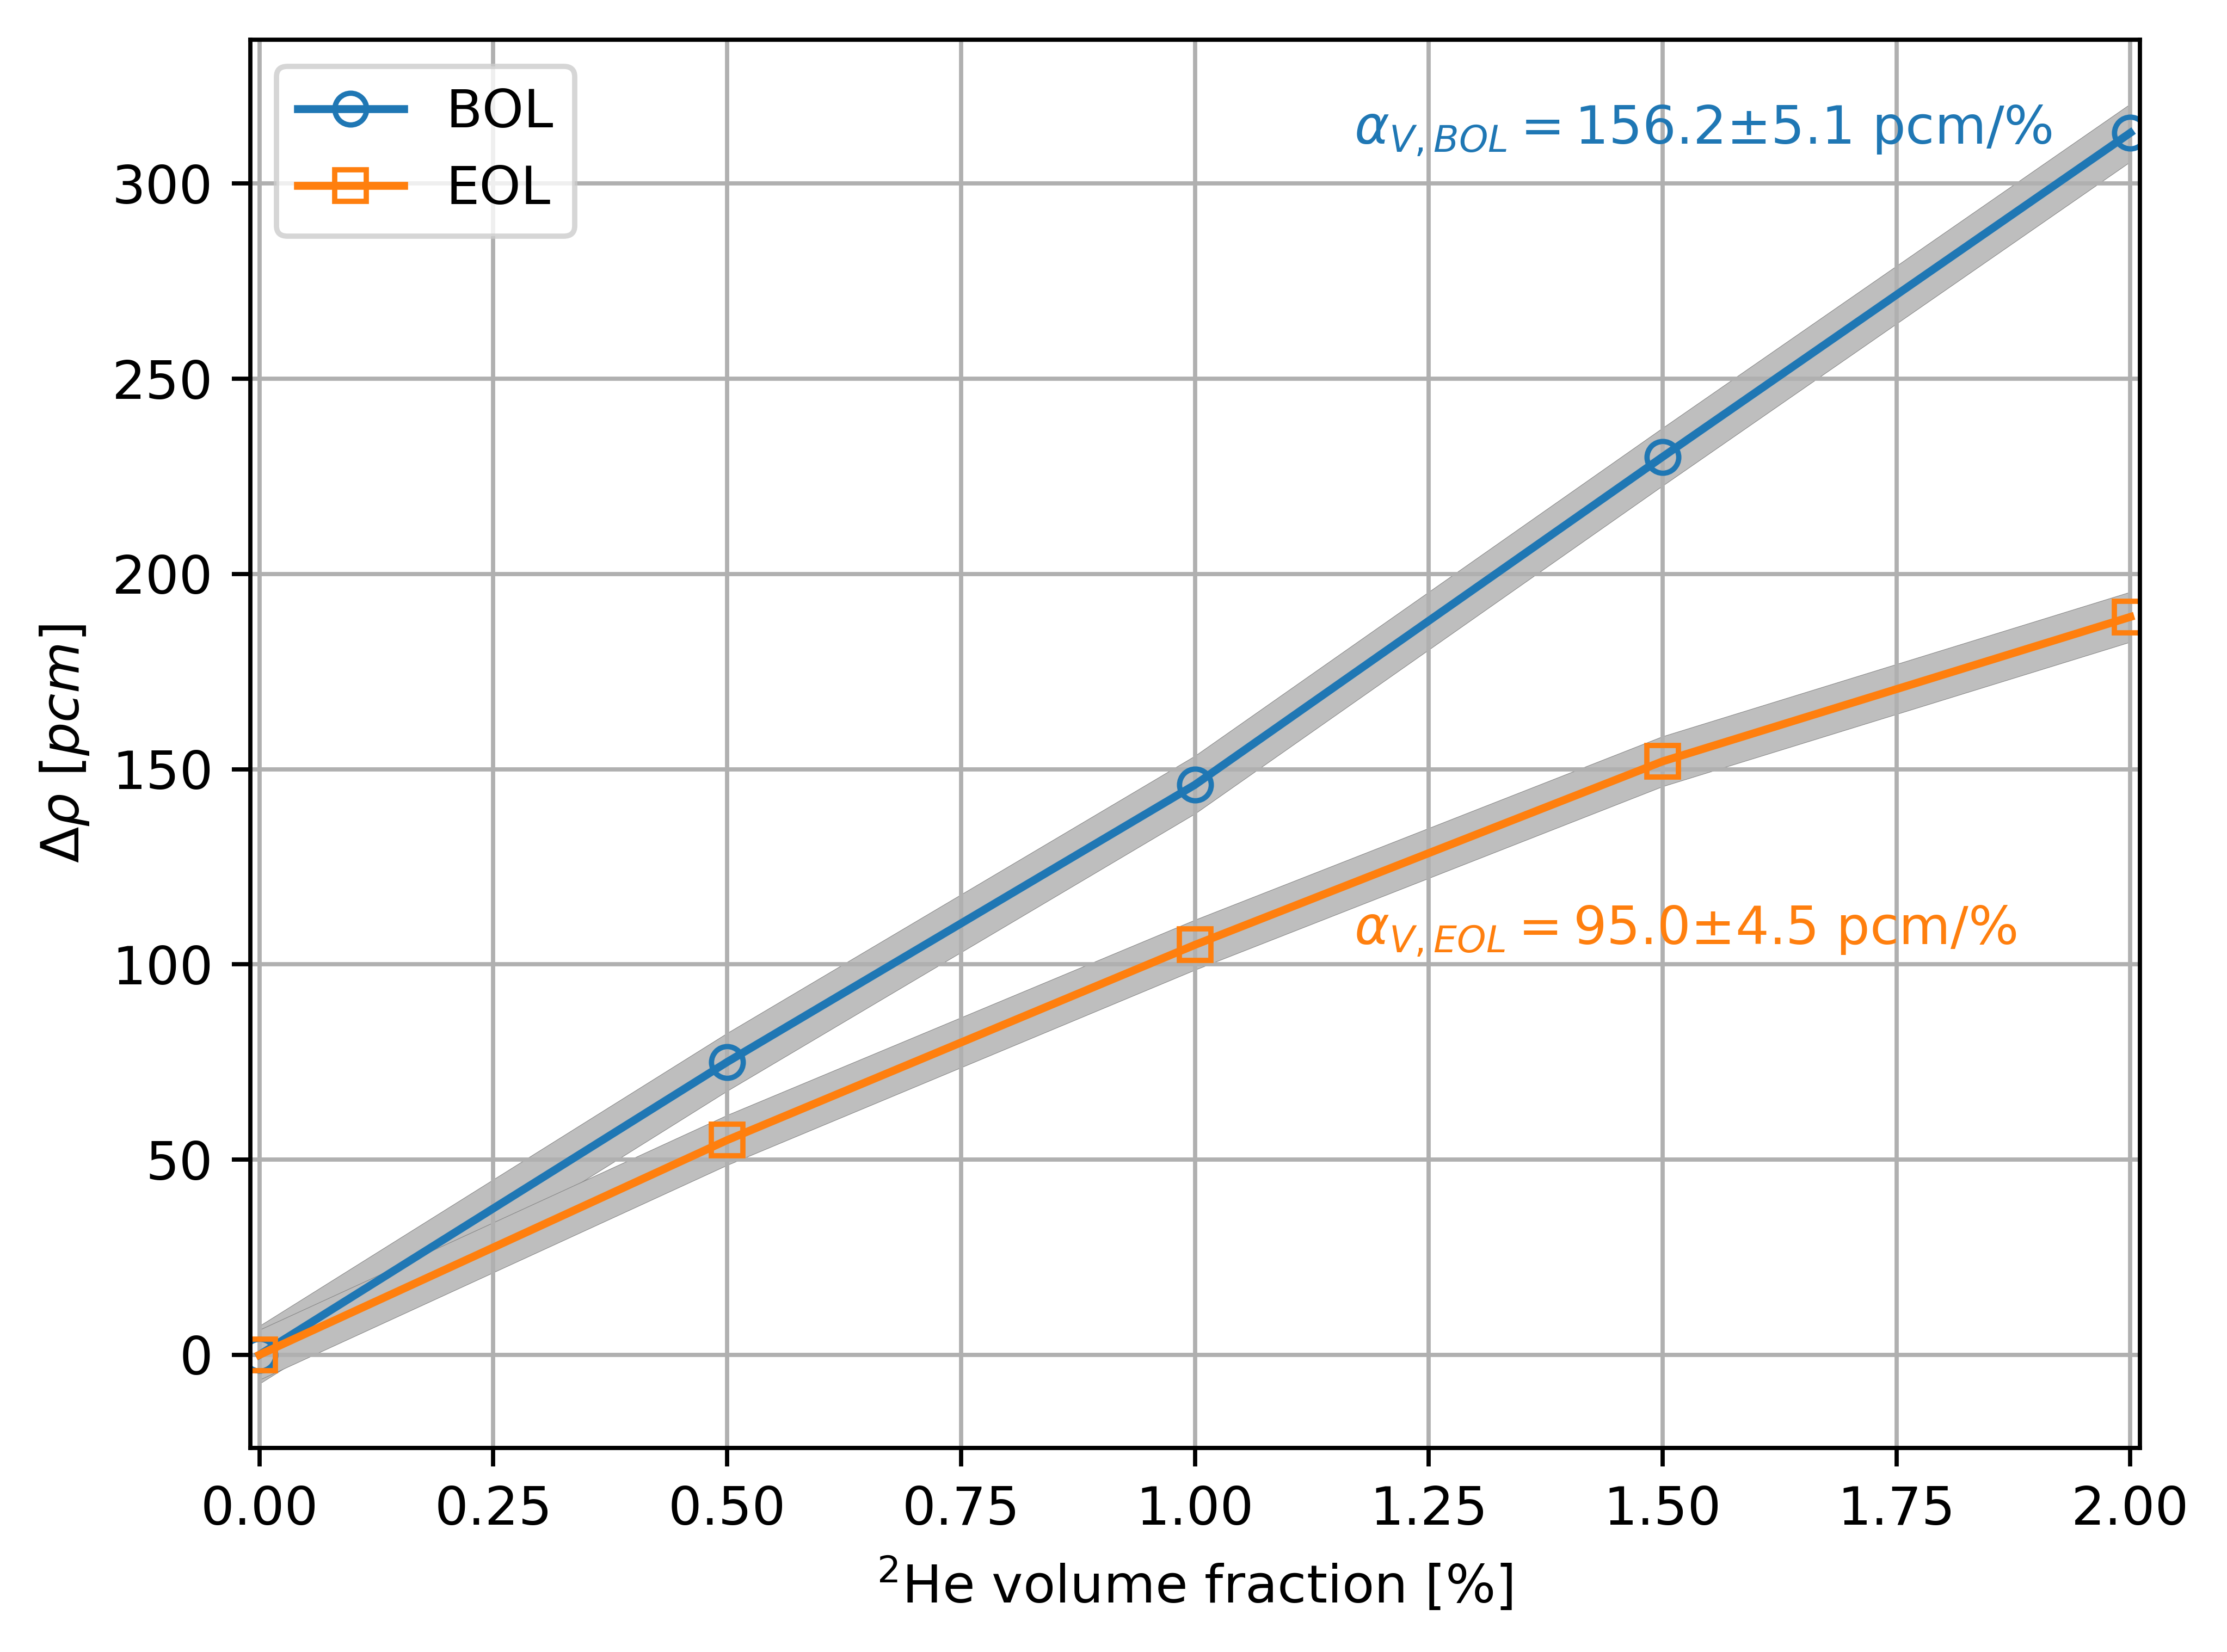
\includegraphics[width=0.85\textwidth]{ch4/saf_par/void_coeff_bol_eol.png}
	\vspace{-4mm}
	\caption{Serpent-calculated reactivity as a function of void volume 
		fraction [\%] in the fuel salt. The uncertainty $\pm\sigma$ region is 
		shaded.}
	\label{fig:void-bol-eol}
\end{figure}

Figure~\ref{fig:void-evo} shows the void coefficient evolution during 25 years 
of operation, taking into account 15 moderator rod reconfigurations. The 
positive void coefficient of reactivity, though not ideal, does not compromise 
the reactor safety, if fuel density change resulted be coupled to a 
change in temperature. And, while some void fraction fluctuations may happen 
due to gaseous fission product production, their generation rates are 
usually almost 
constant. However, a large volume of sparging gas (helium) can be accidentally 
introduced into the \gls{TAP} core in case of the bubble separator 
malfunction. Thus, \emph{the bubble separator must have backup safety 
mechanism} to avoid 
sudden positive negativity insertion in case of the separator failure, 
particularly at the \gls{BOL}. These 
observations from calculating reactivity coefficients should be taken into 
account in the \gls{TAP} \gls{MSR} accident analysis and safety justification.
\begin{figure}[htp!] % replace 't' with 'b' to 
	\centering
	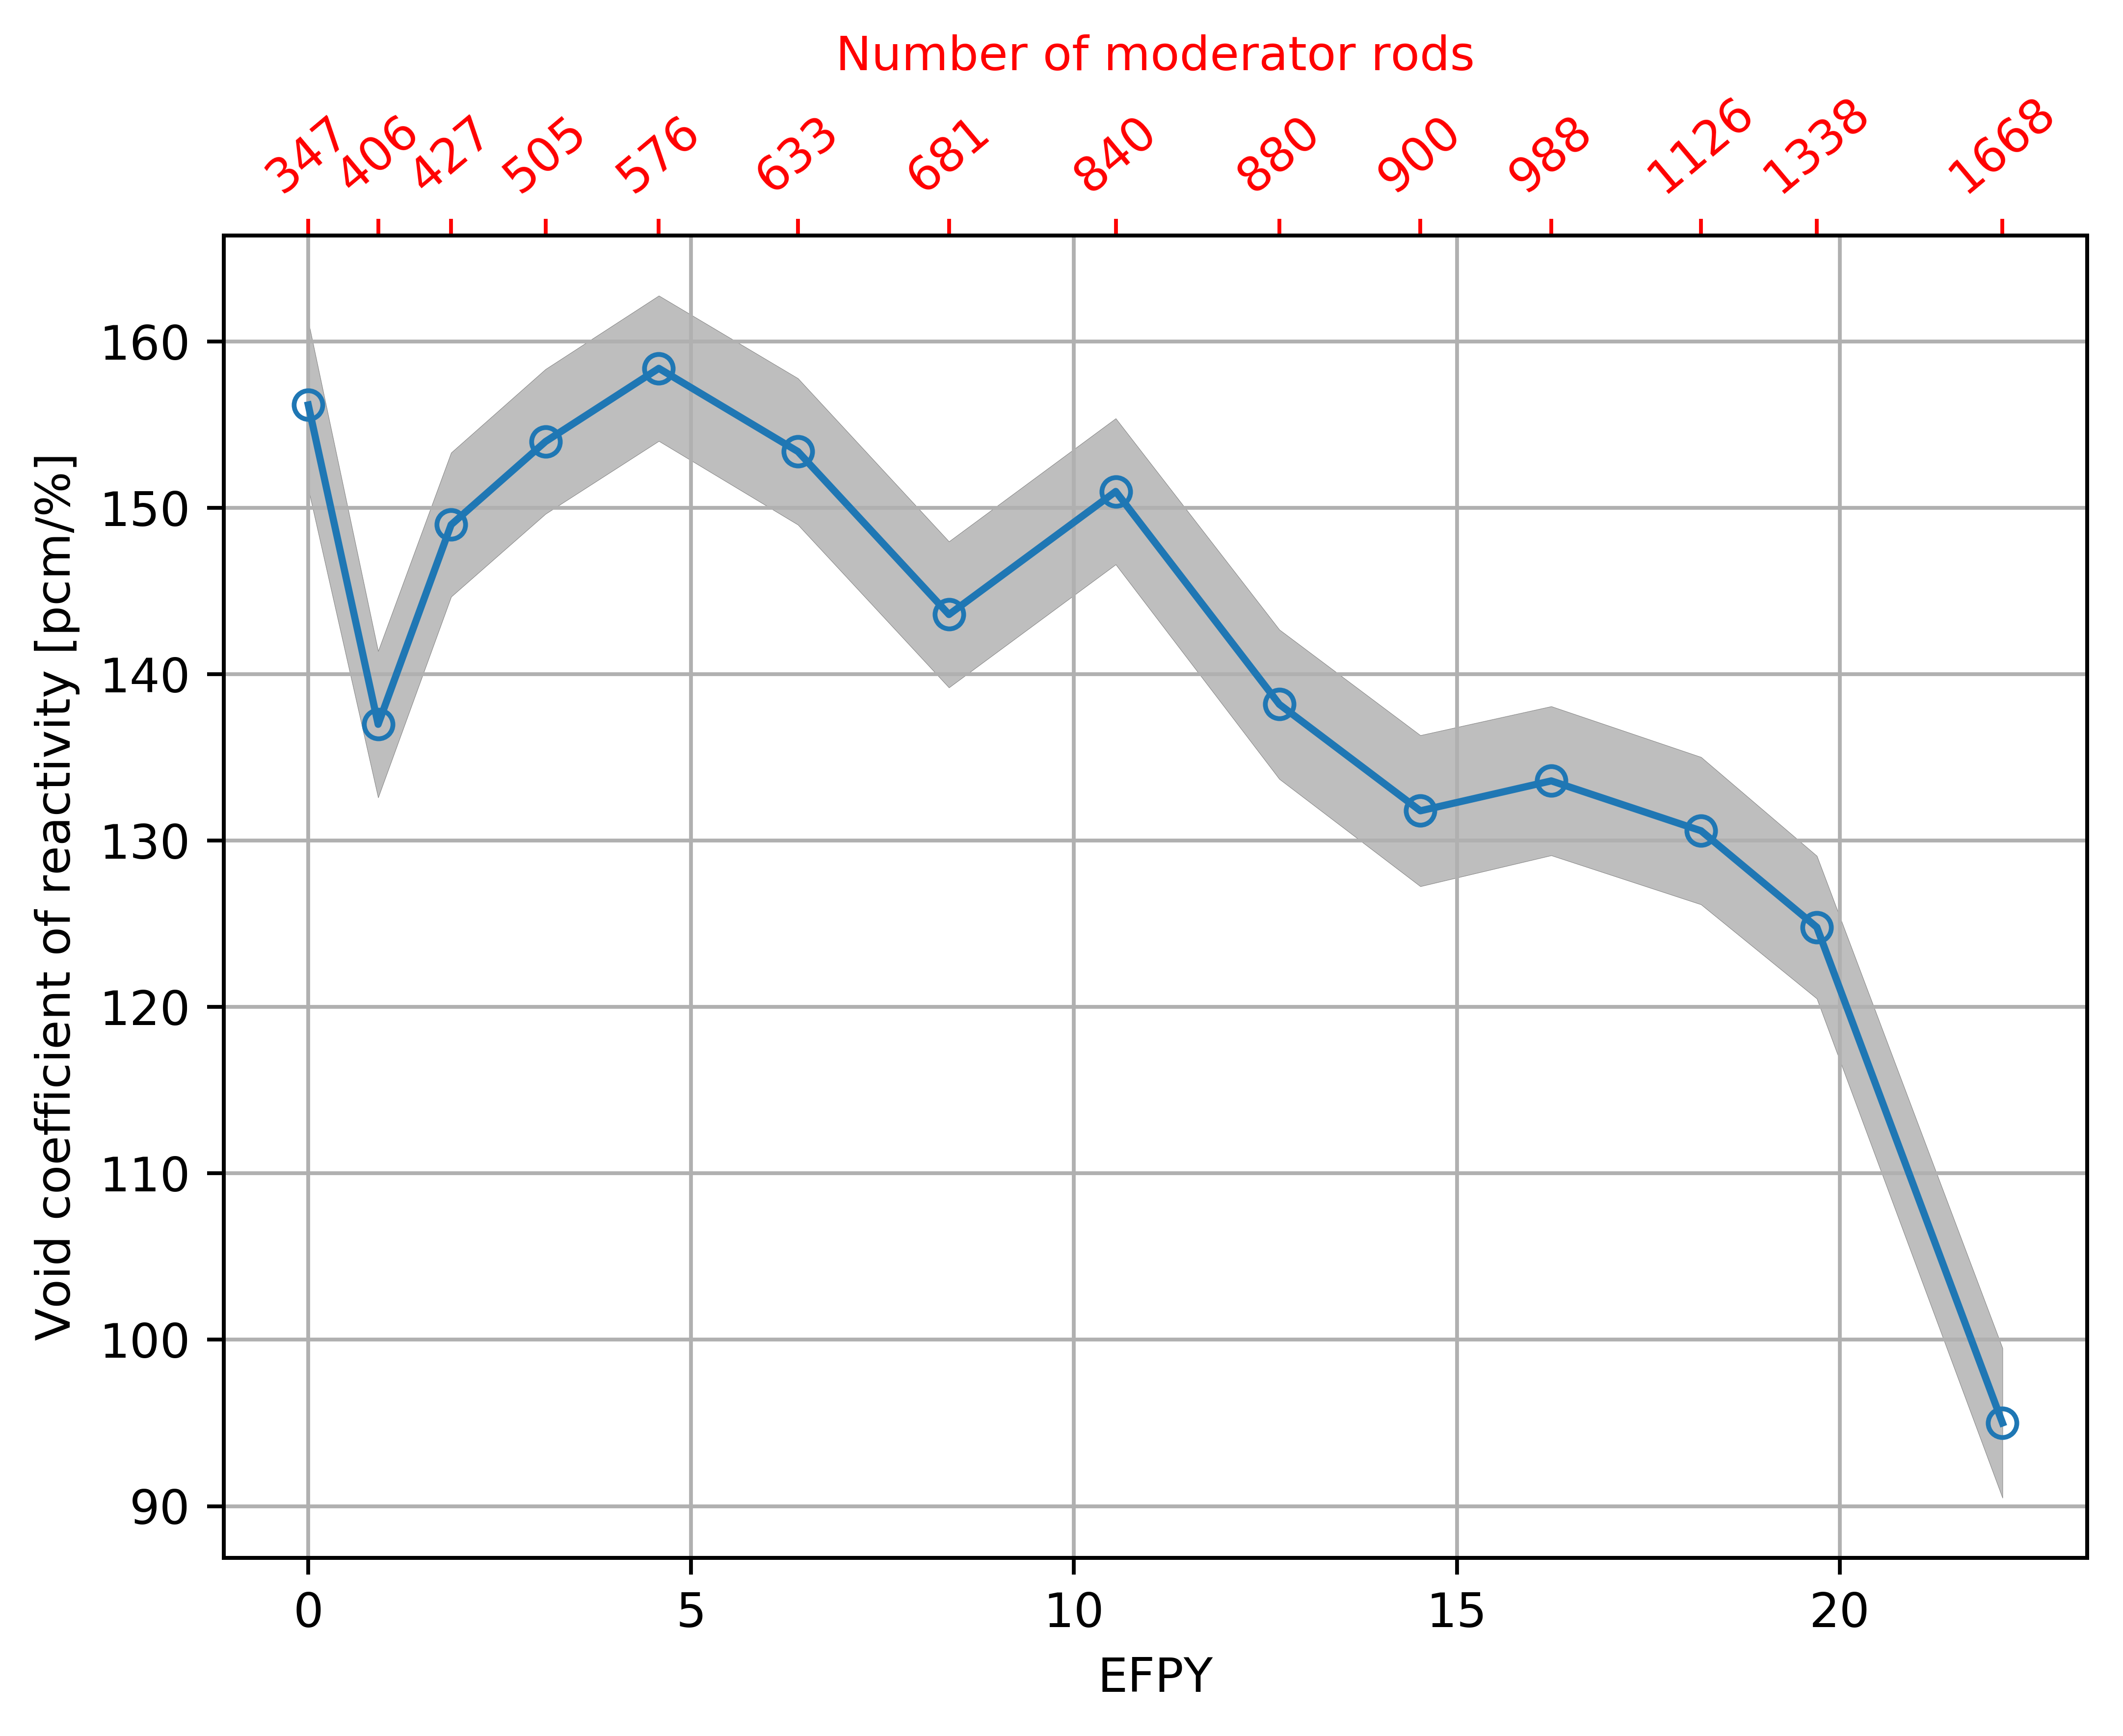
\includegraphics[width=0.94\textwidth]{ch4/saf_par/void_evo.png}
	\caption{Serpent-calculated void coefficient of reactivity as a function 
	of time and number of moderator rods in the \gls{TAP} core. The 
	uncertainty $\pm\sigma$ region is shaded.}
	\label{fig:void-evo}
\end{figure}


\subsection{Reactivity control rod worth}
In the \gls{TAP} concept, control rods perform two main functions: to shut 
down the reactor at any point during operation by negative reactivity 
insertion and to control the excess of reactivity after moderator 
rod reconfiguration during regular maintenance. In an accident, the control 
rods would be dropped down into the core. The total control rod worth 
($\rho_{CRW}$ or CRW) is calculated for various moments during 25 years of 
operation to evaluate neutron spectrum shift influence on the CRW. 

The reactivity worth of all control rods is defined as:
\begin{align}
\rho_{CRW}(pcm) &= \frac{k_{eff}^W - k_{eff}^I}{k_{eff}^W k_{eff}^I}\times 
10^5 \\
\rho_{CRW}(\$) &= \frac{1}{\beta_{eff}} \frac{k_{eff}^W - k_{eff}^I}{k_{eff}^W 
k_{eff}^I}
\intertext{where}
k_{eff}^W &= \mbox{effective multiplication factor when all rods are fully 
	withdrawn} \nonumber \\
k_{eff}^I &= \mbox{effective multiplication factor when all rods are fully 
	inserted} \nonumber  \\
\beta_{eff} &= \mbox{effective delayed neutron fraction.} \nonumber
\end{align}
The statistical error of the  reactivity worth are obtained using formula:
\begin{align}
\delta\rho_{CRW}(pcm) &= \sqrt{\frac{(\delta k_{eff}^W)^2}{(k_{eff}^W)^4} + 
\frac{(\delta k_{eff}^I)^2}{(k_{eff}^I)^4}} \\
\delta\rho_{CRW}(\$) &= \frac{1}{\beta_{eff}}\sqrt{\frac{(\delta 
k_{eff}^W)^2}{(k_{eff}^W)^4} + \frac{(\delta k_{eff}^I)^2}{(k_{eff}^I)^4} + 
\frac{(\delta \beta_{eff})^2 (k_{eff}^W-k_{eff}^I)^2}{\beta_{eff}^2 
(k_{eff}^W k_{eff}^I)^2}}
\intertext{where}
\delta k_{eff}^{W}, \delta k_{eff}^{I}, \delta \beta_{eff} &= 
\mbox{statistical errors from Serpent output.} 
\nonumber
\end{align}

Figure~\ref{fig:crw-evo} demonstrates control rod worth evolution during 25 
years of the \gls{TAP} reactor operation. The cluster of 25 control rods made 
of boron carbide (B$_4$C) provided a reactivity worth of $5.059\pm0.014$ \$ at 
the \gls{BOL}. 
However, spectral shift due to additional moderator rods toward the \gls{EOL} 
leads to significant change in $\rho_{CRW}$. Adding more moderation near 
control rods increases $\rho_{CRW}$ due to the local neutron spectrum 
thermalization (see transition from 347 to 427 moderator rods, 
Figure~\ref{fig:tap-406-681}). 
In contrast, adding moderator rods far away from the control rod positions 
leads to $\rho_{CRW}$ degradation (see transition from 427 to 505 
moderator rods, Figure~\ref{fig:tap-406-681}). On the one hand, the spectrum 
thermalizes and many fission product poisons exhibit larger absorption cross 
sections in the thermal energy range. On the other hand, higher actinides 
(particularly, isotopes of plutonium) are accumulated in the fuel salt which 
deteriorates control rod worth. Overall, $\rho_{CRW}$ decreases to 
$4.472\pm0.015$ \$ at the \gls{EOL}. 
\begin{figure}[htp!] % replace 't' with 'b' to 
	\centering
	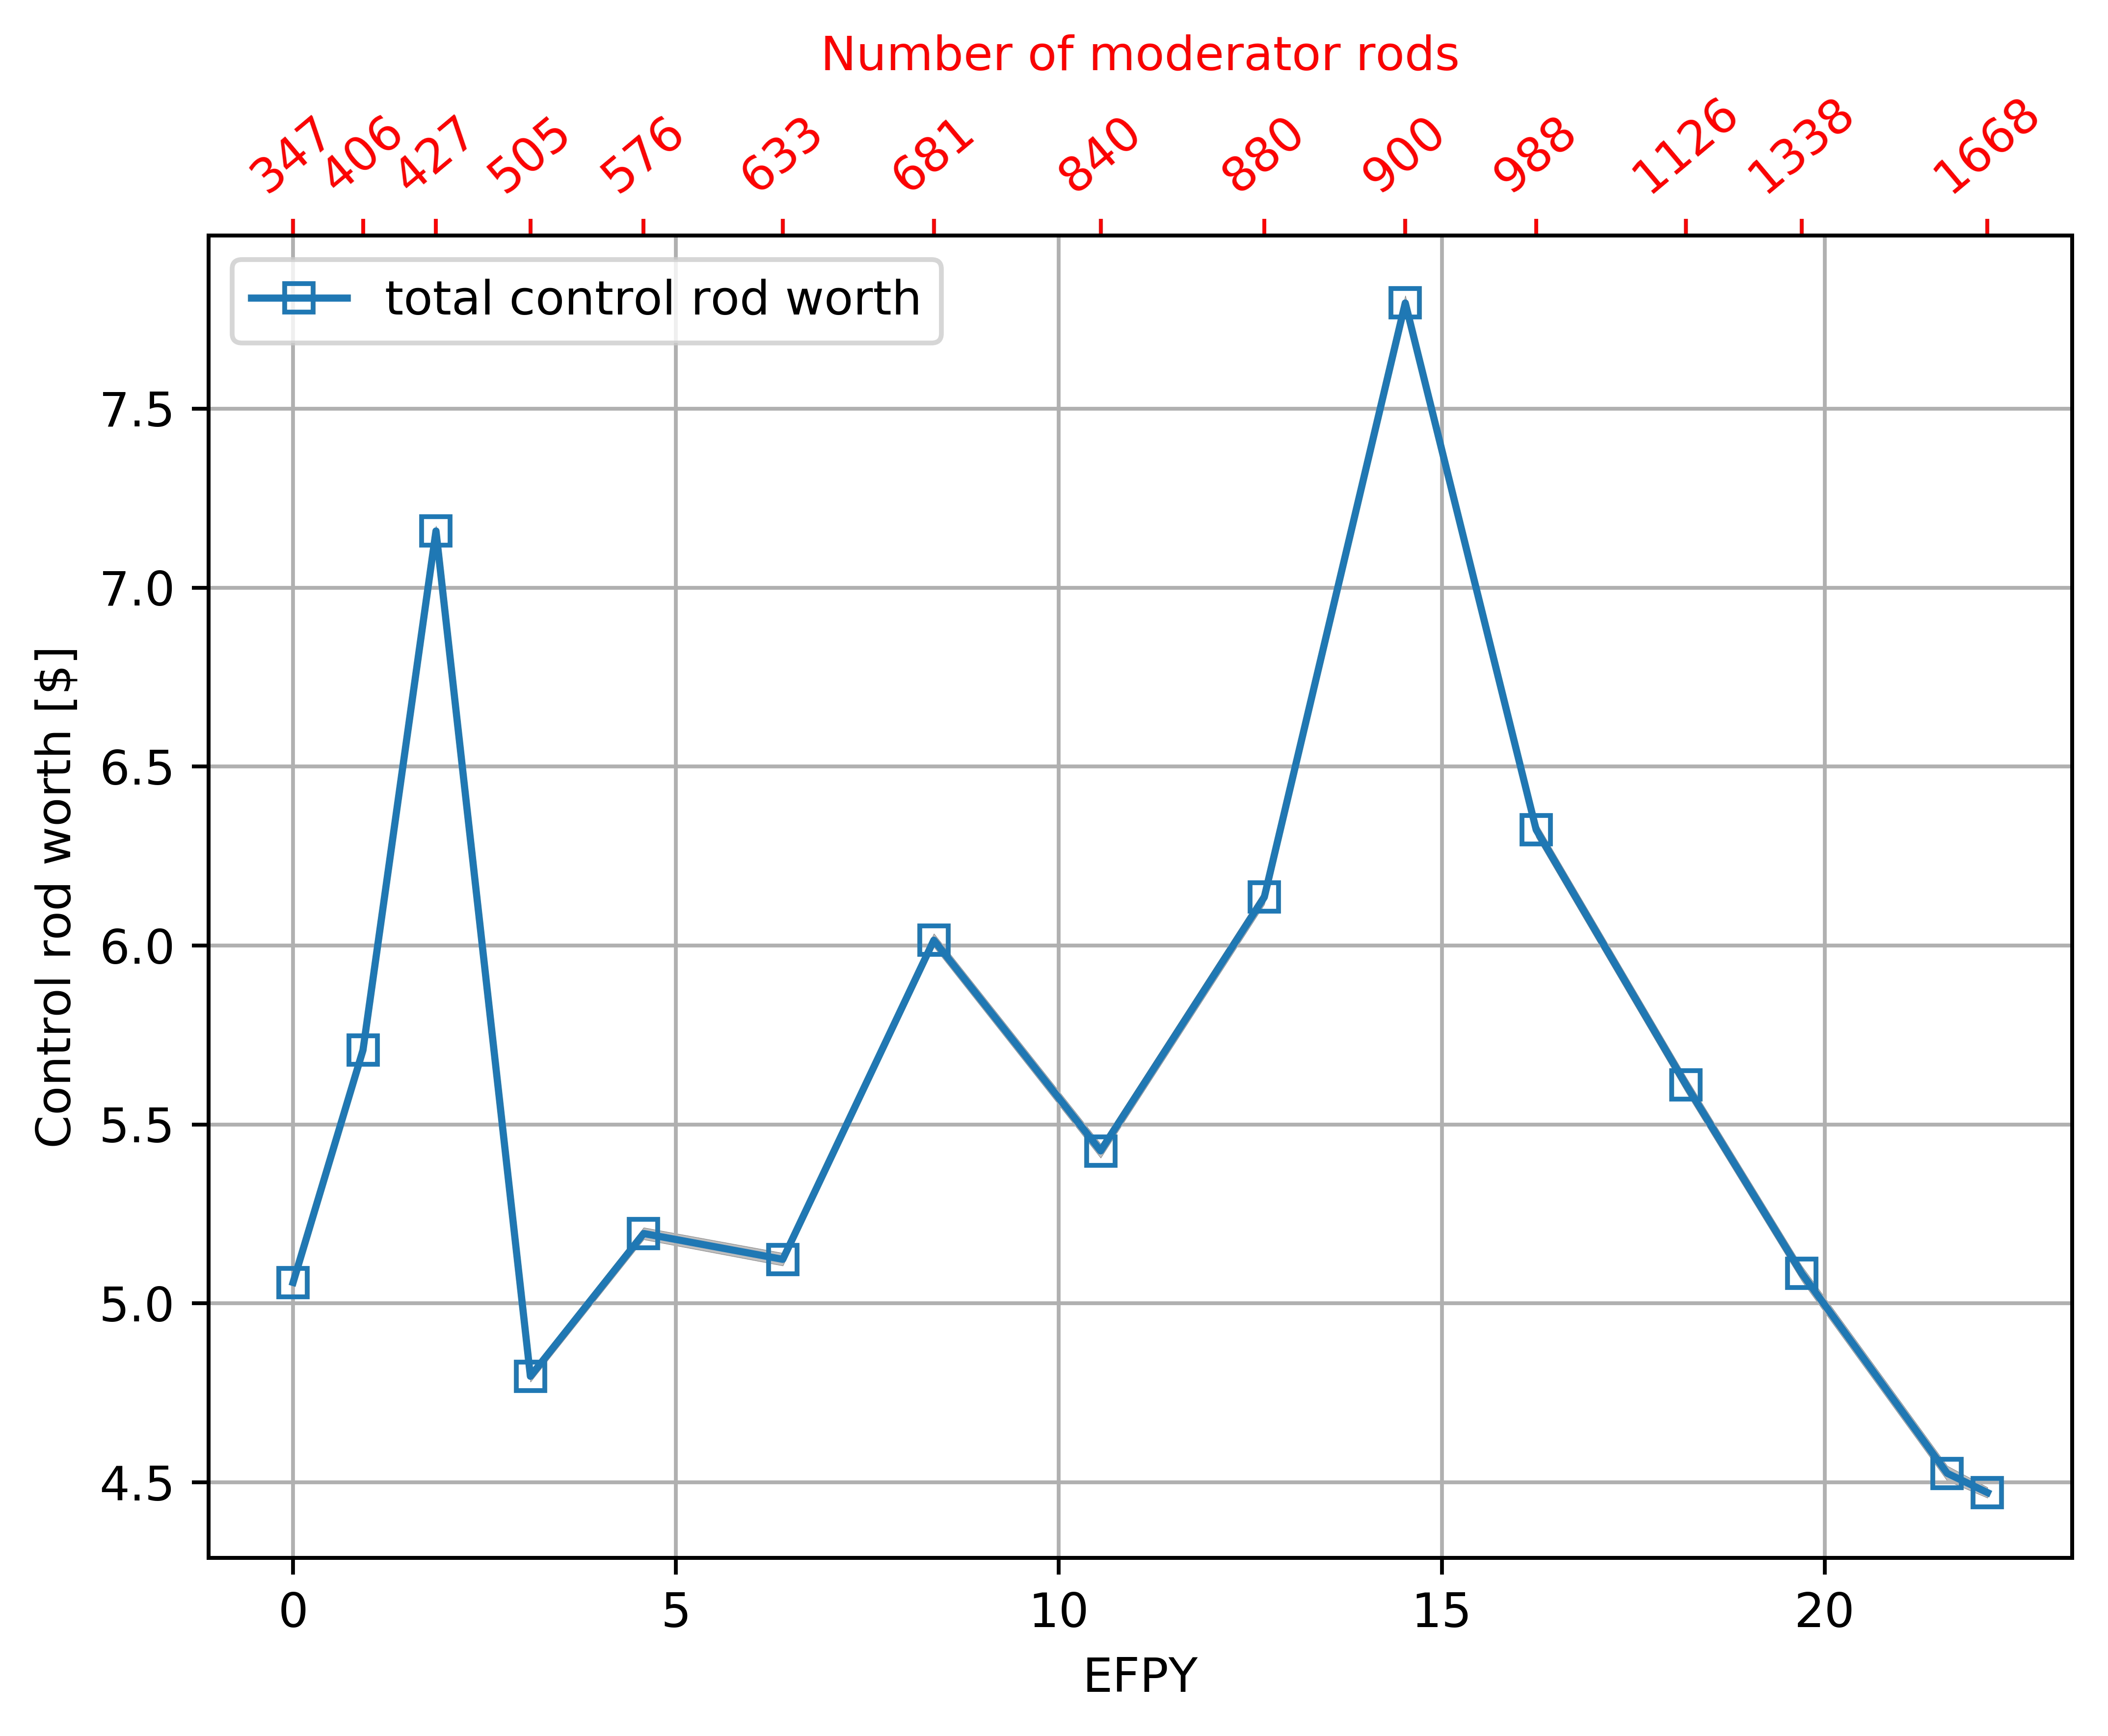
\includegraphics[width=0.85\textwidth]{ch4/saf_par/crw_evo_dollar.png}
		\vspace{-5mm}
	\caption{Serpent-calculated total control rod worth as a function 
		of time and number of moderator rods in the \gls{TAP} core. The 
		uncertainty $\pm\sigma$ region is shaded.}
	\label{fig:crw-evo}
\end{figure}

Overall, the design of the reactivity control system is sufficient to shut 
down the \gls{TAP} reactor at the \gls{BOL}. However, the spectral shift, 
moderator rod reconfigurations, and the change in the salt composition during 
operation drive the total control rod worth below excess reactivity, violating 
reactor safety (insufficient shutdown margin). Thus, the number of control 
rods, their position, or material selection must be revised to make sure that 
the \gls{TAP} reactor could be safely shut down at any moment during 
operation. For example, europium oxide (Eu$_2$O$_3$) might be a better 
absorbing material for the control rods \cite{ashraf_preliminary_2020}.


\subsection{Reactor kinetic parameters}
Most of the neutrons produced in fission are prompt ($>99$\%). But less than 
1\% of neutrons are later emitted by fission products that are called the 
delayed neutron precursors (DNP). The term ``delayed" means, that the neutron 
is emitted due to $\beta$-decay with half-lives in the range from few 
milliseconds up to 1 minute. Even though, the number of delayed neutrons per 
fission neutron is quite small ($<1$\% for most fissile isotopes), they play 
an essential role in the nuclear reactor control. Delayed neutrons presence 
changes the dynamic time response of a reactor to reactivity change from 
$10^{-7}$ s to 10 s, making it controllable by reactivity control system such 
as control rods. In nuclear library JEFF-3.1.2, delayed nuclear precursors are 
divided into 8 groups, each with different characteristic half-life, 
$\lambda_i$. The delayed neutron fraction, $\beta_i$, is defined as the 
fraction of all fission neutrons that appears as delayed neutrons in the 
$i^{th}$ group.

It is crucial to study kinetic parameter dynamics because the fuel salt 
composition changes with time and new actinides appear in the fuel, which 
alters the emission of delayed neutrons. Figures~\ref{fig:beta-eol} 
and \ref{fig:lamda-eol} show precursor-group-wise delayed neutron fraction 
(DNF, $\beta_i$) and decay constant ($\lambda_i$) evolution during 25 years of 
\gls{TAP} \gls{MSR} operation. The effective delayed neutron fraction 
($\beta_{eff}$) in the \gls{TAP} core decreased dramatically from 
$7.245\times10^{-3}$($\pm0.5$\%) at the \gls{BOL} to 
$4.564\times10^{-3}$($\pm0.6$\%) at the \gls{EOL} ($-37$\%). 

\begin{figure}[htbp!] % replace 't' with 'b' to 
	\centering
	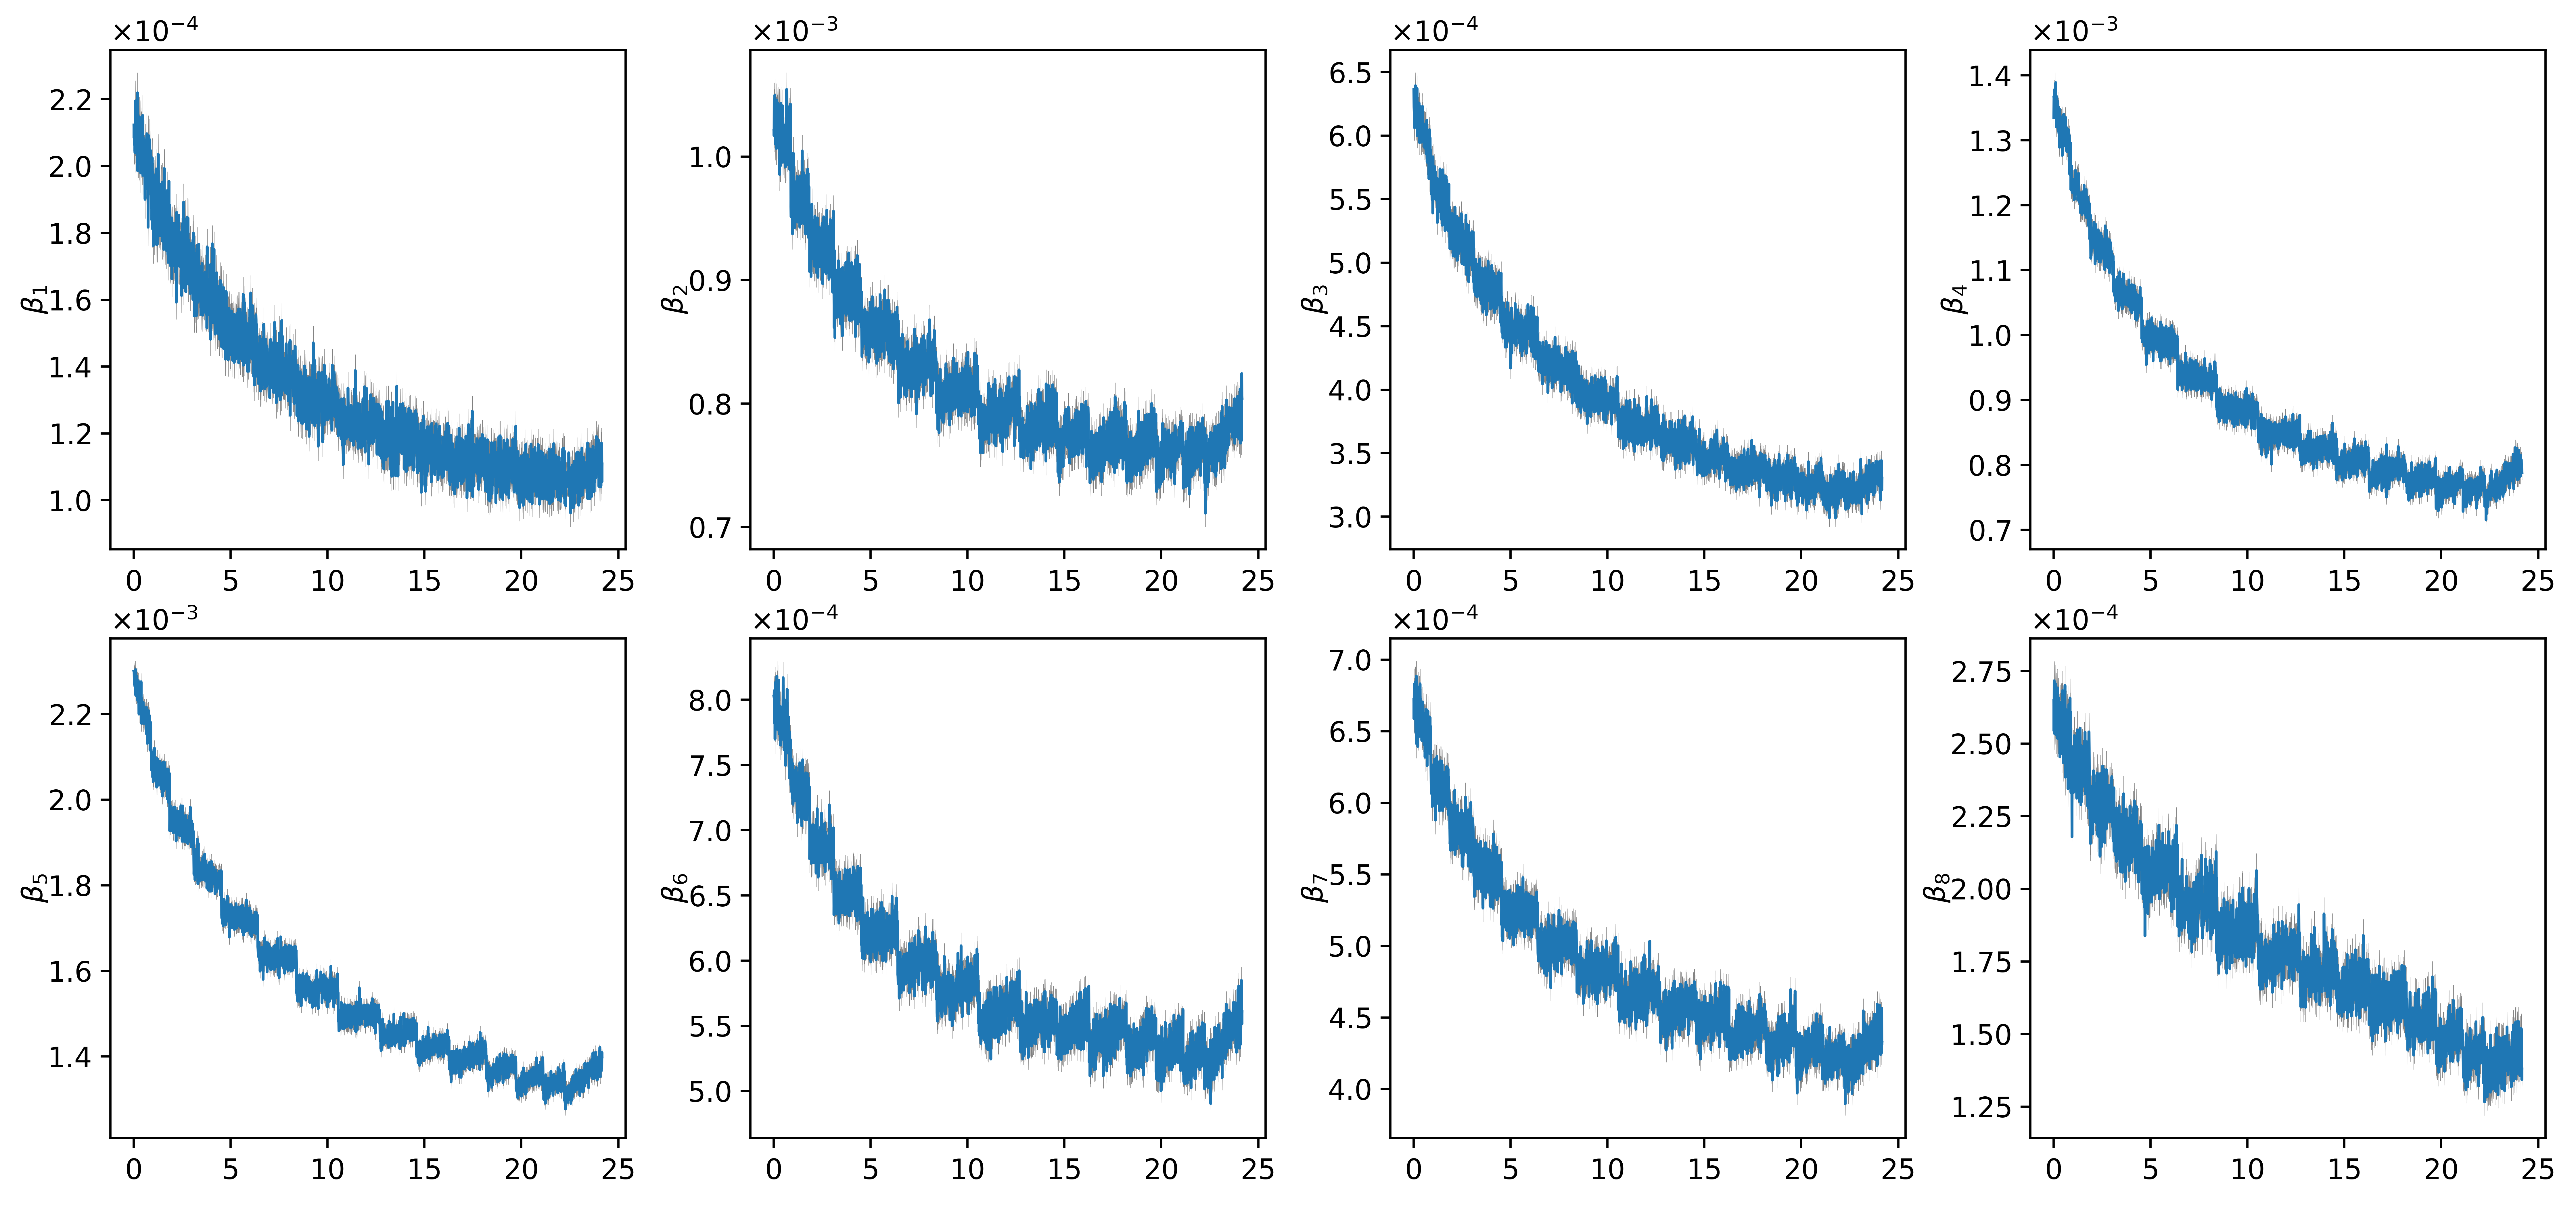
\includegraphics[width=\textwidth]{ch4/saf_par/betas_evo.png}
		\vspace{-5mm}
	\caption{Evolution of the precursor-group-wise delayed neutron fraction 
	($\beta_i$) as a function of time for the \gls{TAP} \gls{MSR}. The 
	uncertainty $\pm\sigma$ 
	region is shaded.}
	\label{fig:beta-eol}
\end{figure}
\begin{figure}[hbbp!] % replace 't' with 'b' to 
	\centering
	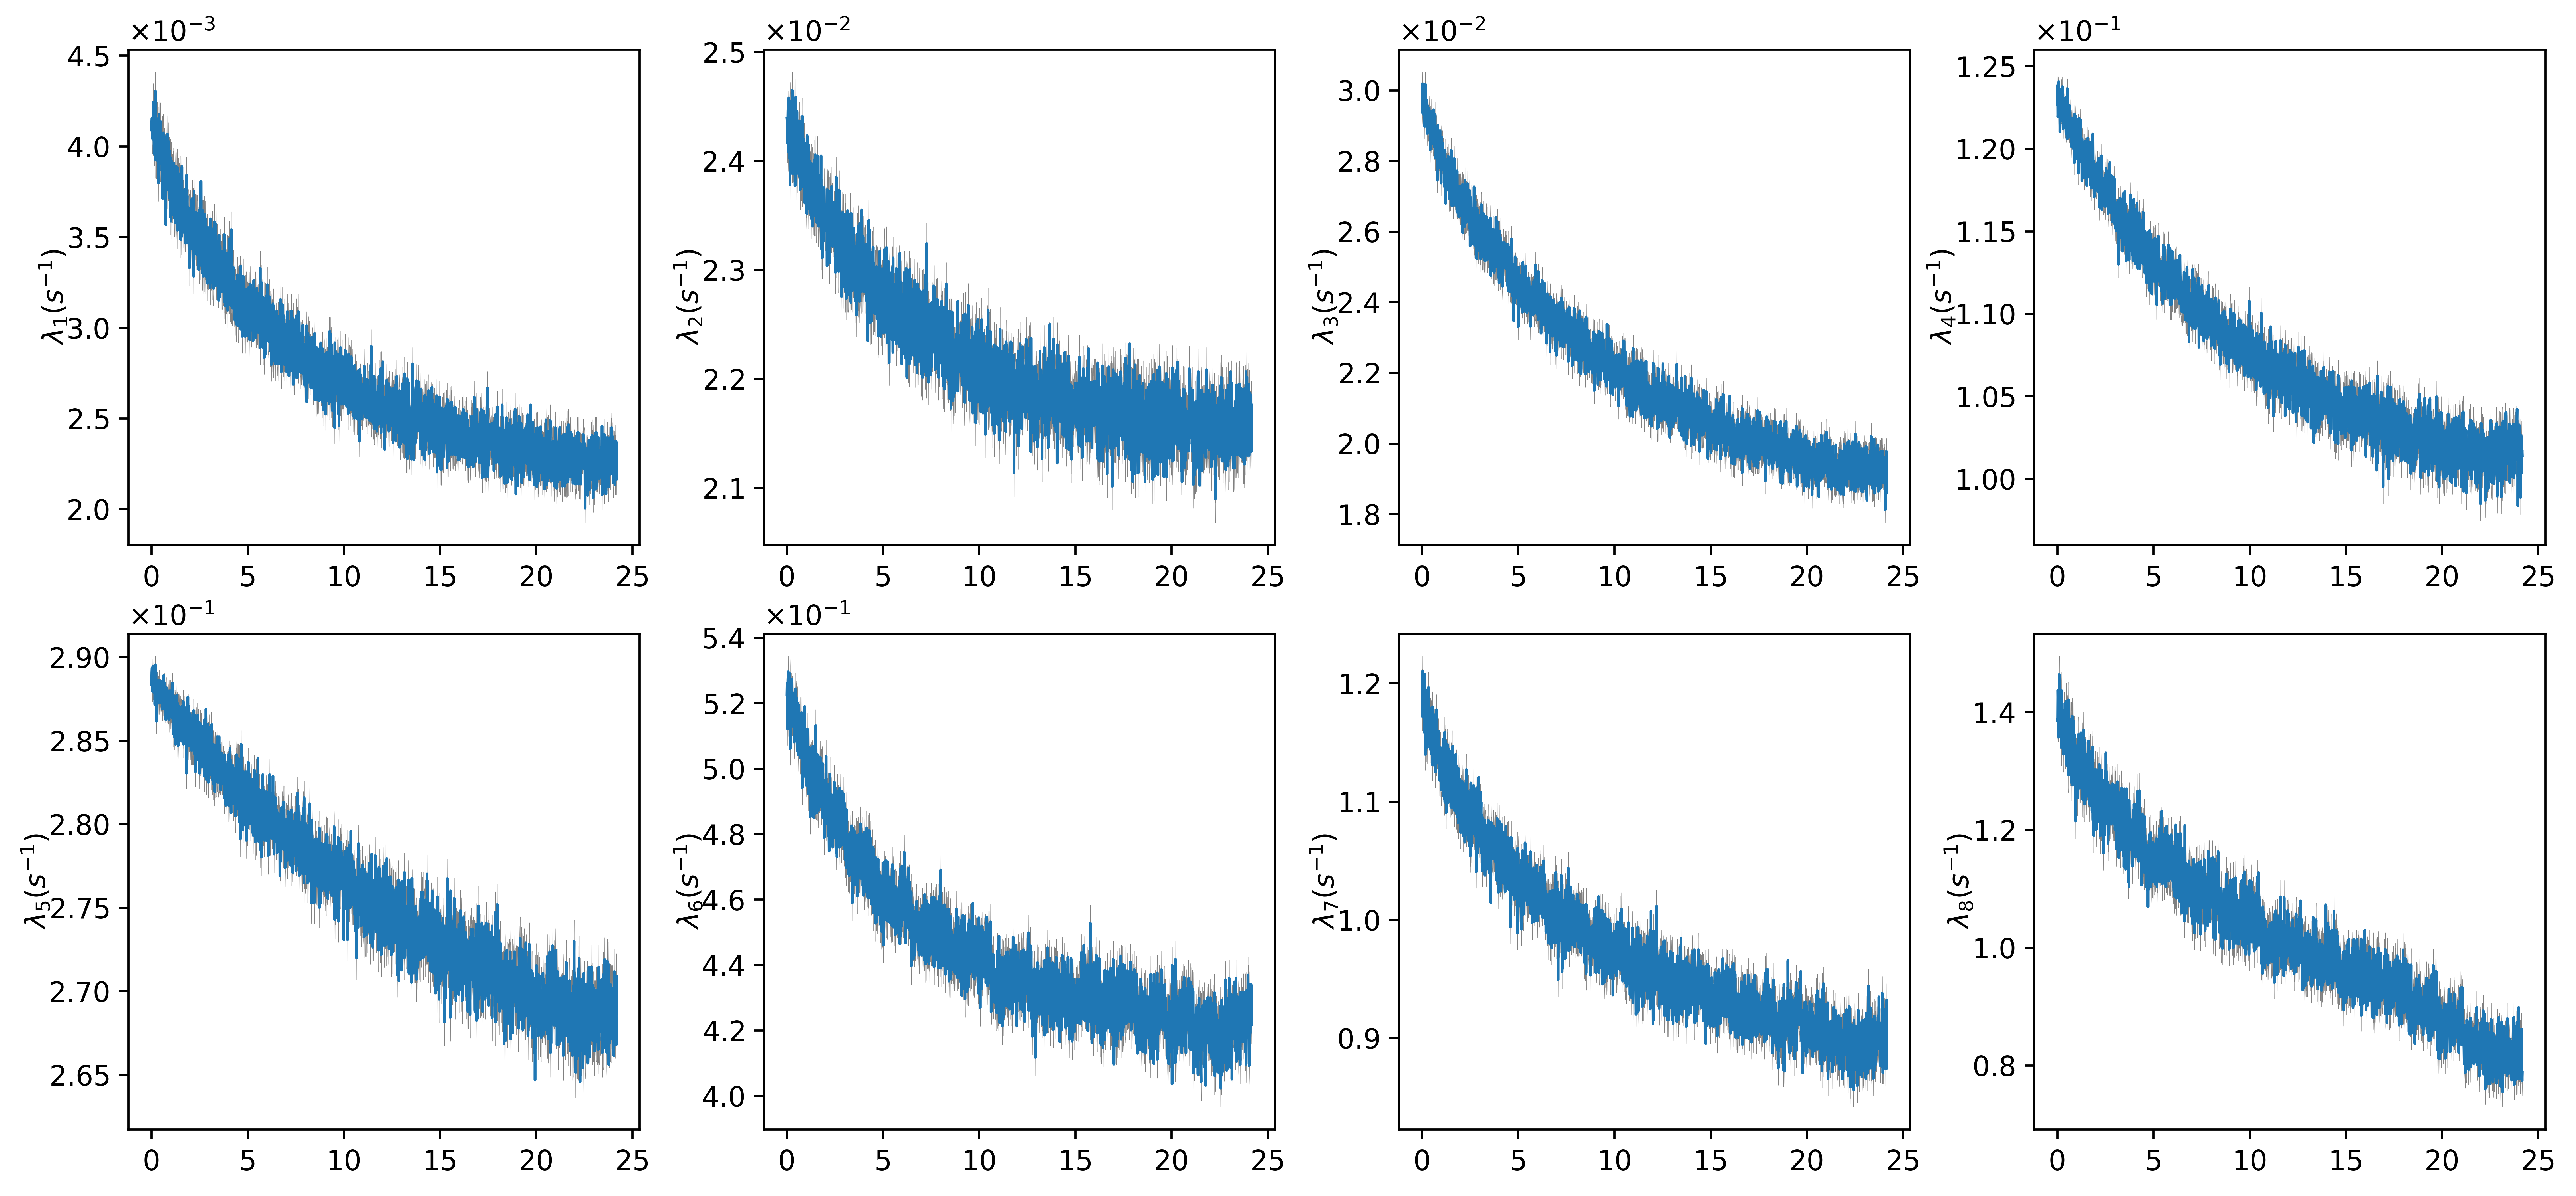
\includegraphics[width=\textwidth]{ch4/saf_par/lambdas_evo.png}
	\vspace{-5mm}
	\caption{Evolution of the precursor-group-wise decay constant 
	($\lambda_i$) as a function of time for the \gls{TAP} \gls{MSR}. The 
	uncertainty $\pm\sigma$ region is shaded.}
	\label{fig:lamda-eol}
\end{figure}

Similarly, the effective precursor decay constant ($\lambda_{eff}$) slipped 
slightly from $0.481$ $s^{-1}$($\pm0.8$\%) to $0.468$ $s^{-1}$($\pm1.1$\%) 
during 25 years of operation. During operation, the concentration of $^{235}$U 
decreases, and the concentration of fissile plutonium isotopes (e.g., 
$^{239}$Pu) 
increases. Notably, $^{239}$Pu emits about 2.5 times fewer delayed neutrons 
than $^{235}$U; delayed neutron yields are 0.00664 and 0.01650 for the 
$^{239}$Pu and $^{235}$U, respectively. Thus, as fuel salt burnup increases, 
delayed neutron emission is controlled by plutonium isotopes (e.g., $^{239}$Pu 
and $^{241}$Pu) and decreases with time. All decay constants show a slight 
decrease toward the \gls{EOL} due to the reactor spectrum hardening. This 37\% 
decline in the effective delayed neutron fraction and 3\% decline in the 
effective precursor decay constant must be taken into account in the \gls{TAP} 
design accident analysis and safety justification.



\newpage
\section{Concluding remarks}
This chapter demonstrated SaltProc v1.0 capabilities for lifetime-long fuel 
salt depletion simulations applied to the \gls{TAP} \gls{MSR}. 
Section~\ref{sec:tap_design_sum} summarized the \gls{TAP} \gls{MSR} core and 
fuel salt reprocessing system details that inform the SaltProc model 
(Section~\ref{sec:tap_model}).
%I validated SaltProc v1.0 capabilities for lifetime-long (25 years) depletion 
%calculation with assumed gas ideal removal efficiency against 
%SCALE/ChemTriton 
%simulation by Betzler \emph{et al.} \cite{betzler_assessment_2017-1}.  
%Additionally, this chapter presented isotopic composition evolution for 
%various, non-ideal gas removal efficiency (e.g, $<100$\% of the target 
%isotope 
%is removed).
 
Section~\ref{sec:ben-valid} presented lifetime-long depletion simulations with 
SaltProc v1.0. The 25-year simulation assumed ideal removal efficiency 
(e.g., 100\% of target neutron poison is being removed at the end of each 
depletion step). This validation effort demonstrated good agreement with a 
reference ORNL report \cite{betzler_assessment_2017-1}. Full-core 3D 
SaltProc/Serpent analysis showed that spectrum hardening over the first 13 
years of operation produces a sufficient amount of fissile plutonium to 
achieve the fuel salt burnup of 76.3 MWd/kgU after 22.5 years of operation. 
SaltProc-calculated inventories of major heavy isotopes at the \gls{EOL} are 
consistent with results in the literature. The difference in mass between 
SaltProc and the reference was only 3\% and 4\% for fissile ($^{235}$U, 
$^{239}$Pu, $^{241}$Pu) and non-fissile ($^{236}$U, $^{238}$U, $^{238}$Pu, 
$^{240}$Pu, $^{242}$Pu) isotopes, respectively. Finally, the 
SaltProc-calculated feed rate is 460.8 kg of UF$_4$ per year, which consistent 
with 480 kg/y reported by Betzler \emph{et al.} 
\cite{betzler_assessment_2017-1}

The time step refinement study in Section~\ref{sec:time-refinement} showed 
that accurate uranium isotopic content predictions could be obtained with a 
relatively long depletion time step (6- or 12-day). However, the significant 
absolute difference in plutonium mass at the \gls{EOL} ($\approx10$ kg for a 
6-day step) could be a safeguards issue, as this represents more than one 
significant quantity (8 kg) over the reactor lifetime. Overall, to get 
accurate plutonium isotopic content without raising proliferation issues, a 
3-day depletion time step must be used.

Section~\ref{sec:long-term-real} of this chapter demonstrated SaltProc v1.0 
for a 25-year depletion simulation with a realistic, physics-based noble gas 
removal efficiency. When identifying a reasonable mathematical model 
for realistic gas removal efficiency ($\epsilon$), the liquid phase mass 
transfer coefficient ($K_L$) demonstrated a strong correlation with 
$\epsilon$. Thus, SaltProc simulations using different $K_L$ in validity range 
from 0.0847 to 8.4667 $mm/s$ (corresponding $^{135}$Xe removal efficiency 
$\epsilon\in [0.031,0.915]$) showed that the larger liquid phase mass transfer 
coefficient and corresponding higher noble gas extraction efficiency provided 
significant neutronics benefit, better fuel utilization, and longer time 
between shutdowns for moderator rod reconfiguration. Notably, the larger mass 
transfer coefficient also provides a slightly more thermal neutron spectrum 
because poisonous \glspl{FP} ($^{135}$Xe) absorb fewer thermal neutrons. In 
the following chapters, the results of these realistic depletion simulations 
will be used for short-term transient simulations and safety parameter 
analysis. 

Finally, this chapter demonstrated safety and operational parameter evolution 
during 25 years of the \gls{TAP} \gls{MSR} operation. In general, the safety 
of the reactor worsens with time due to actinides and \glspl{FP} accumulating 
in the fuel salt. Shifting neutron spectrum from epithermal to thermal by 
periodically adding more moderator rods also has a negative influence on 
crucial safety an operational characteristics. These observations must be 
taken into account in the \gls{TAP} \gls{MSR} designing, accident analysis, 
and safety justification.